% Options for packages loaded elsewhere
\PassOptionsToPackage{unicode}{hyperref}
\PassOptionsToPackage{hyphens}{url}
%
\documentclass[
]{book}
\usepackage{amsmath,amssymb}
\usepackage{lmodern}
\usepackage{ifxetex,ifluatex}
\ifnum 0\ifxetex 1\fi\ifluatex 1\fi=0 % if pdftex
  \usepackage[T1]{fontenc}
  \usepackage[utf8]{inputenc}
  \usepackage{textcomp} % provide euro and other symbols
\else % if luatex or xetex
  \usepackage{unicode-math}
  \defaultfontfeatures{Scale=MatchLowercase}
  \defaultfontfeatures[\rmfamily]{Ligatures=TeX,Scale=1}
\fi
% Use upquote if available, for straight quotes in verbatim environments
\IfFileExists{upquote.sty}{\usepackage{upquote}}{}
\IfFileExists{microtype.sty}{% use microtype if available
  \usepackage[]{microtype}
  \UseMicrotypeSet[protrusion]{basicmath} % disable protrusion for tt fonts
}{}
\makeatletter
\@ifundefined{KOMAClassName}{% if non-KOMA class
  \IfFileExists{parskip.sty}{%
    \usepackage{parskip}
  }{% else
    \setlength{\parindent}{0pt}
    \setlength{\parskip}{6pt plus 2pt minus 1pt}}
}{% if KOMA class
  \KOMAoptions{parskip=half}}
\makeatother
\usepackage{xcolor}
\IfFileExists{xurl.sty}{\usepackage{xurl}}{} % add URL line breaks if available
\IfFileExists{bookmark.sty}{\usepackage{bookmark}}{\usepackage{hyperref}}
\hypersetup{
  pdftitle={Tablas y graficos con R y R Studio},
  pdfauthor={Roberto Gil Saura  },
  hidelinks,
  pdfcreator={LaTeX via pandoc}}
\urlstyle{same} % disable monospaced font for URLs
\usepackage{color}
\usepackage{fancyvrb}
\newcommand{\VerbBar}{|}
\newcommand{\VERB}{\Verb[commandchars=\\\{\}]}
\DefineVerbatimEnvironment{Highlighting}{Verbatim}{commandchars=\\\{\}}
% Add ',fontsize=\small' for more characters per line
\usepackage{framed}
\definecolor{shadecolor}{RGB}{248,248,248}
\newenvironment{Shaded}{\begin{snugshade}}{\end{snugshade}}
\newcommand{\AlertTok}[1]{\textcolor[rgb]{0.94,0.16,0.16}{#1}}
\newcommand{\AnnotationTok}[1]{\textcolor[rgb]{0.56,0.35,0.01}{\textbf{\textit{#1}}}}
\newcommand{\AttributeTok}[1]{\textcolor[rgb]{0.77,0.63,0.00}{#1}}
\newcommand{\BaseNTok}[1]{\textcolor[rgb]{0.00,0.00,0.81}{#1}}
\newcommand{\BuiltInTok}[1]{#1}
\newcommand{\CharTok}[1]{\textcolor[rgb]{0.31,0.60,0.02}{#1}}
\newcommand{\CommentTok}[1]{\textcolor[rgb]{0.56,0.35,0.01}{\textit{#1}}}
\newcommand{\CommentVarTok}[1]{\textcolor[rgb]{0.56,0.35,0.01}{\textbf{\textit{#1}}}}
\newcommand{\ConstantTok}[1]{\textcolor[rgb]{0.00,0.00,0.00}{#1}}
\newcommand{\ControlFlowTok}[1]{\textcolor[rgb]{0.13,0.29,0.53}{\textbf{#1}}}
\newcommand{\DataTypeTok}[1]{\textcolor[rgb]{0.13,0.29,0.53}{#1}}
\newcommand{\DecValTok}[1]{\textcolor[rgb]{0.00,0.00,0.81}{#1}}
\newcommand{\DocumentationTok}[1]{\textcolor[rgb]{0.56,0.35,0.01}{\textbf{\textit{#1}}}}
\newcommand{\ErrorTok}[1]{\textcolor[rgb]{0.64,0.00,0.00}{\textbf{#1}}}
\newcommand{\ExtensionTok}[1]{#1}
\newcommand{\FloatTok}[1]{\textcolor[rgb]{0.00,0.00,0.81}{#1}}
\newcommand{\FunctionTok}[1]{\textcolor[rgb]{0.00,0.00,0.00}{#1}}
\newcommand{\ImportTok}[1]{#1}
\newcommand{\InformationTok}[1]{\textcolor[rgb]{0.56,0.35,0.01}{\textbf{\textit{#1}}}}
\newcommand{\KeywordTok}[1]{\textcolor[rgb]{0.13,0.29,0.53}{\textbf{#1}}}
\newcommand{\NormalTok}[1]{#1}
\newcommand{\OperatorTok}[1]{\textcolor[rgb]{0.81,0.36,0.00}{\textbf{#1}}}
\newcommand{\OtherTok}[1]{\textcolor[rgb]{0.56,0.35,0.01}{#1}}
\newcommand{\PreprocessorTok}[1]{\textcolor[rgb]{0.56,0.35,0.01}{\textit{#1}}}
\newcommand{\RegionMarkerTok}[1]{#1}
\newcommand{\SpecialCharTok}[1]{\textcolor[rgb]{0.00,0.00,0.00}{#1}}
\newcommand{\SpecialStringTok}[1]{\textcolor[rgb]{0.31,0.60,0.02}{#1}}
\newcommand{\StringTok}[1]{\textcolor[rgb]{0.31,0.60,0.02}{#1}}
\newcommand{\VariableTok}[1]{\textcolor[rgb]{0.00,0.00,0.00}{#1}}
\newcommand{\VerbatimStringTok}[1]{\textcolor[rgb]{0.31,0.60,0.02}{#1}}
\newcommand{\WarningTok}[1]{\textcolor[rgb]{0.56,0.35,0.01}{\textbf{\textit{#1}}}}
\usepackage{longtable,booktabs,array}
\usepackage{calc} % for calculating minipage widths
% Correct order of tables after \paragraph or \subparagraph
\usepackage{etoolbox}
\makeatletter
\patchcmd\longtable{\par}{\if@noskipsec\mbox{}\fi\par}{}{}
\makeatother
% Allow footnotes in longtable head/foot
\IfFileExists{footnotehyper.sty}{\usepackage{footnotehyper}}{\usepackage{footnote}}
\makesavenoteenv{longtable}
\usepackage{graphicx}
\makeatletter
\def\maxwidth{\ifdim\Gin@nat@width>\linewidth\linewidth\else\Gin@nat@width\fi}
\def\maxheight{\ifdim\Gin@nat@height>\textheight\textheight\else\Gin@nat@height\fi}
\makeatother
% Scale images if necessary, so that they will not overflow the page
% margins by default, and it is still possible to overwrite the defaults
% using explicit options in \includegraphics[width, height, ...]{}
\setkeys{Gin}{width=\maxwidth,height=\maxheight,keepaspectratio}
% Set default figure placement to htbp
\makeatletter
\def\fps@figure{htbp}
\makeatother
\setlength{\emergencystretch}{3em} % prevent overfull lines
\providecommand{\tightlist}{%
  \setlength{\itemsep}{0pt}\setlength{\parskip}{0pt}}
\setcounter{secnumdepth}{5}
\usepackage{booktabs}
\usepackage{booktabs}
\usepackage{longtable}
\usepackage{array}
\usepackage{multirow}
\usepackage{wrapfig}
\usepackage{float}
\usepackage{colortbl}
\usepackage{pdflscape}
\usepackage{tabu}
\usepackage{threeparttable}
\usepackage{threeparttablex}
\usepackage[normalem]{ulem}
\usepackage{makecell}
\usepackage{xcolor}
\usepackage{caption}
\usepackage{graphicx}
\usepackage{siunitx}
\usepackage{hhline}
\usepackage{calc}
\usepackage{tabularx}
\usepackage{adjustbox}
\usepackage{hyperref}
\ifluatex
  \usepackage{selnolig}  % disable illegal ligatures
\fi
\usepackage[]{natbib}
\bibliographystyle{apalike}

\title{Tablas y graficos con R y R Studio}
\author{Roberto Gil Saura
\includegraphics{data/portada.png}}
\date{Última actualización: 2021-06-06}

\begin{document}
\maketitle

{
\setcounter{tocdepth}{1}
\tableofcontents
}
\hypertarget{prefacio}{%
\chapter*{Prefacio}\label{prefacio}}
\addcontentsline{toc}{chapter}{Prefacio}

Todavía recuerdo cuando hace unos años descubrí R \citep{R-base} -lejos queda ya aquel 2000- y me pareció una herramienta valiosa para mi trabajo, pero que no era para mí. La percibí para usuarios programadores y no para analistas o científicos de datos, como gusta llamar hoy en día a estos trabajadores del dato. Sin embargo, hace tres años (2018)y tras una etapa en la que centré mis energías y esfuerzos en mi PhD, redescubrí esta herramienta y no sólo ella, también R Studio y todo el trabajo que se había realizado en estos últimos años. Quedé gratamente impresionado y me puse manos a la obra porque vi un enorme potencial en la misma para lo que era mi trabajo actual. Una de las cuestiones fundamentales que aprecié es que las dos herramientas ya no sólo se enfocaban (probablemente nunca lo habían hecho) sólo a los programadores, sino que se apreciaba mucho el enfoque a analistas con todo tipo de formación y con escasos conocimientos de programación, pero que no temían enfrentarse a algo que les iba a reportar eficiencia en su trabajo y un enorme potencial de evolución. Con el paso del tiempo fui descubriendo todo lo que R y R Studio podrían hacer por mí (y por mis alumnos), y lo que ganaba / ahorraba en mi trabajo y en las soluciones que podía ofrecer a mis colegas y/o clientes. Y ahí empezó todo.

En este documento, sólo pongo el foco en dos aspectos fundamentales en el mundo de la investigación de mercados cuantitativa: las tablas de contingencia y los gráficos, en sus diferentes modalidades y con sus diferentes sabores, básico y avanzados, visuales y no tan visuales; todo ello condimentado y aderezado con una cantidad de paquetes suplementarios y la inestimable ayuda de esos programadores que desinteresadamente ceden su trabajo a la comunidad. En especial aquí debo agradecer a Gregory Demin, Joshua Kunst y a Yihui Xie su desinteresada colaboración en la creación de diferentes paquetes y utilidades que han servidor para poder plasmar toda la información que aquí se desarrolla.

\begin{quote}
\textbf{Cita}
\end{quote}

Gil-Saura, R., 2021. Tablas y gráficos con R y R Studio. 1st ed.~{[}ebook{]} València: InvestigaOnline.com. ISBN: 978-84-09-29382-7;disponible en: \url{https://tables.investigaonline.com}.

\begin{quote}
\textbf{Licencia}
\end{quote}

© Textos y gráficos: Roberto Gil-Saura (\href{mailto:robertogil@investigaonline.com}{\nolinkurl{robertogil@investigaonline.com}})

Cualquier forma de reproducción, distribución, comunicación pública o transformación de esta obra solo podrá ser realizada con la autorización expresa del autor bajo los términos abajo descritos.

1ª edición: Valencia, 2021 ISBN: 978-84-09-29382-7 Última actualización: 2021-06-06

This work is licensed under a Creative Commons Attribution-NonCommercial-ShareAlike 4.0 Unported License (CC BY-NC-SA 4.0) \url{http://creativecommons.org/licenses/by-nc/4.0/} In short: Roberto Gil-Saura retains the Copyright but you are free to reproduce, reblog, remix and modify the content only under the same license to this one. You may not use this work for commercial purposes but permission to use this material in nonprofit teaching is still granted, provided the authorship and licensing information here is displayed.


\includegraphics{data/88x31.png}

\hypertarget{tse01}{%
\chapter{Introducción}\label{tse01}}

\hypertarget{por-quuxe9-este-libro}{%
\section{¿Por qué este libro?}\label{por-quuxe9-este-libro}}

La respuesta más simple a la pregunta ¿Por qué este libro? es que no hay libros dedicados a ilustrar y mostrar cómo hacer tablas de contingencia y gráficos a partir de esas tablas usando R; hablando más específicamente usando \texttt{expss} y \texttt{highcharter}. Por otro lado, a partir de mi experiencia y de muchos años dedicado al mundo de la investigación y la docencia (mi hobbie personal) encontré el tiempo y la motivación para escribirlo. Quería crear un recurso que fuera diferente del resto de textos con el mismo contenido aproximado y porque creo que para que las ideas se difundan y adopten ampliamente, deben percibirse de manera amigable y fácil de entender, lo que tiene por qué estar reñido con una baja calidad científica y teórica. Si algo se percibe como complejo e intimidante, solo pocos creerán que ese recurso es apropiado para ellos. Así pues, y aunque todos los análisis requieren las habilidades propias de una persona acostumbrada a manejar fuentes de datos variadas, creo realmente que el recurso es extremadamente sencillo, funcional, comprensible y válido para todos.

¿No es acaso necesario y nos viene muy bien el poder utilizar macros en software como Microsoft Office© o sintaxis en IBM SPSS© ? Pues esta es la respuesta, mostrar de una forma sencilla la posibilidad de que el usuario pueda utilizar código R \citep{R-base} en sus análisis de datos, que le permitan ir mucho más allá de lo que ofrecen las herramientas básicas comerciales.

Además, la elección de R no es casual:

\begin{itemize}
\item
  La primera razón para elegir R es que es un programa extremadamente potente para manipular y analizar datos. Su popularidad en alza lo ha convertido en el software de referencia para estadísticas y análisis en muchas disciplinas, y se enseña cada vez más en muchas universidades. R se ha convertido en uno los de los estándares de facto de la industria del proceso, análisis y visualización de datos, dentro de ese nuevo ámbito que es al analítica o ciencia de datos, que está dando cabida a muchos profesionales de nueva creación y en la que nos estamos integrando muchos otros que provenimos de ámbitos diferentes.
\item
  La segunda razón para seleccionar R es que es independiente de la plataforma (puede usarla en Windows© , Mac o Unix) y es gratis y por ello no se deb invertir un euro en licencias, mantenimientos o actualizaciones. Los proveedores de software comercial pueden brindar soporte y ofrecer algún tipo de garantía, pero eso es secundario. No se puede superar el precio y la funcionalidad de R. R se enriquece por el hecho de que muchas personas de todo el mundo contribuyen y comparten su propio trabajo en forma de funcionalidades incluidas en paquetes de lo más variado y que llegan al mercado con una celeridad imposible para cualquier otro software comercial. Asimismo, R tiene recursos de ayuda inigualables, tanto en línea como físicos. Hay muchos foros en línea, listas de correo electrónico, grupos de interés, foros, blogs y sitios web llenos de información rica sobre R. Además, cada año se publican cada vez más muchos libros de R de excelente calidad. Lo que realmente se valora de R, es su carácter de código abierto, lo que permite (si sabes) ver el código por dentro alejándose de ser una caja negra.
\end{itemize}

\hypertarget{para-quiuxe9n-este-libro}{%
\section{¿Para quién este libro?}\label{para-quiuxe9n-este-libro}}

El presente documento enfoca e introduce al usuario de investigación (fundamentalmente de Investigación de Mercados) en la creación de información analítica y reproducible utilizando scripting con \emph{Markdown}, que permita obtener cualquier tipo de tabla resumen de datos o cualquier análisis que pueda hacer utilizando código R.

Este manual ha sido redactado pensando en los usuarios que trabajan de forma conjunta con R Studio y R. Por tanto, se asume que el usuario estará familiarizado con el uso de ambas aplicaciones y se le supone conocimiento básico de cómo funcionar con ellas. No obstante, al inicio de la sección 3, el usuario puede encontrar unos sencillos rudimentos de como trabajar para iniciarse con el trabajo de R Studio y por extensión de R.

\hypertarget{estructura-del-documento}{%
\section{Estructura del documento}\label{estructura-del-documento}}

En investigación de mercado, las tablas de contingencia o cruzadas probablemente sean el análisis de datos más predominante de todos los utilizados, complementado por una potente visualización en forma de gráfico de esos datos. Se pretende dotar al usuario de de las herramientas básicas que le permitan reproducir cualquier tipo de cuadro o tabla, de tipo marginal o cruzada, con medidas estadísticas básicas, combinando estadísticos y frecuencias o porcentajes, o realizar pruebas de significación estándar, así como la reproducción de los gráficos que se adaptarían a esas tablas. La estructura del manual se adapta por tanto a este objetivo, organizándose de la siguiente forma:

\begin{itemize}
\tightlist
\item
  esta introducción al manual, donde también se ayuda a la instalación de ambas herramientas de trabajo R y R Studio;
\item
  una sección que dedicamos a introducir al lector en el lenguaje R; no se pretende hacer un revisión exhaustiva del lenguaje, sino simplemente enumerar los términos y conceptos que serán necesarios para entender el funcionamiento de las tablas y el manejo y gestión de las mismas;
\item
  una sección donde se introduce al usuario en la escritura de sencillas órdenes que como resultado obtendrán un cuadro o tabla;
\item
  una sección dedicada a la creación de las tablas cruzadas;
\item
  una sección dedicada a tablas más especiales, que denominaremos multi dimensionales;
\item
  una sección dedicada a la generación de otras tablas auxiliares: cuadros, escalas, etc.;
\item
  un epígrafe que describirá las pruebas básicas de significación que se utilizan en las tablas de contingencia;
\item
  una sección dedicada a los gráficos;
\item
  un epígrafe dedicado a operaciones con tablas, entre filas y/o columnas y a mejorar la visualización de las tablas y obtener gráficos a partir de estas operaciones especiales, ampliando el conjunto de paquetes a utilizar y combinando sus funcionalidades;
\item
  por último, una sección complementaria más de lenguaje R, para saber cómo se incluyen las condiciones para cualquier tipo de selección de datos.
\end{itemize}

Para seguir este manual, tal y como hemos comentado anteriormente, asumimos que el usuario conoce mínimamente R y R Studio y que ha constatado su necesidad de reproducir tipos de tabla que ha visto que son posibles de obtener en Quantum, Minitab, Systat, Star, SPSS o BarbWin entre otros. Explicaremos los rudimentos básicos de trabajo en R, pero adecuados a su uso en R Studio, con una primera introducción a cómo integramos R en su flujo de trabajo.

Agradecemos expresamente a Gregory \citet{expss}, desarrollador del paquete \textbf{\texttt{expss}} de R por su desinteresado trabajo en código abierto que permite reproducir e ir más allá de los cuadros resumen creados; al igual que a Joshua \citet{highcharter}, desarrollador del paquete \textbf{\texttt{highcharter}} por su excelente aportación en el mundo de la graficación con la creación del \emph{wrapper} para la librería Highchart, renombrada y conocida librería de gráficos JavaScipt que permite su uso en R. Y no puedo acabar esta sección sin mencionar al equipo de R Studio y en particular a Yihui \citet{bookdown}, que con sus diferentes aportaciones, permite que esta obra llegue a vuestros ojos en las condiciones que lo hace usando el paquete \textbf{\texttt{bookdown}} desde R Studio.

\hypertarget{instalaciuxf3n-de-r-y-r-studio}{%
\section{Instalación de R y R Studio}\label{instalaciuxf3n-de-r-y-r-studio}}

Para poder seguir el manual de forma correcta, deberemos tener instalados R y R Studio. Sigue estos pasos para poder hacerlo en Windows. Si es sobre Linux o MacOS, busca información sobre cómo instalarlo específicamente en tu versión. Es muy sencillo, pero con una imágenes se ve mejor.

\hypertarget{instalaciuxf3n-de-r-en-windows}{%
\subsection{Instalación de R en Windows}\label{instalaciuxf3n-de-r-en-windows}}

Los pasos son los siguientes:

\begin{enumerate}
\def\labelenumi{\arabic{enumi}.}
\item
  Abre el siguiente enlace: \url{https://cran.r-project.org/}
\item
  Selecciona la opción ``Download R for Windows''.
\end{enumerate}

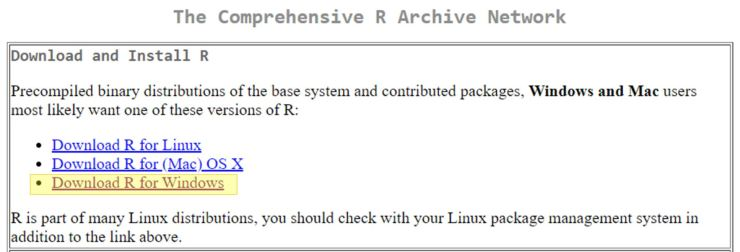
\includegraphics{data/01.png}

\begin{enumerate}
\def\labelenumi{\arabic{enumi}.}
\setcounter{enumi}{2}
\tightlist
\item
  En la nueva página seleccione ``base''.
\end{enumerate}

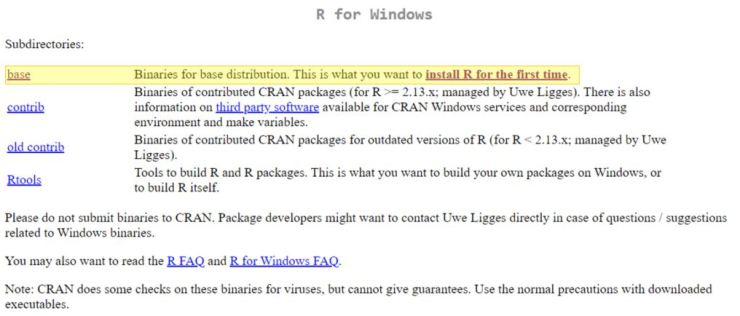
\includegraphics{data/02.png}

\begin{enumerate}
\def\labelenumi{\arabic{enumi}.}
\setcounter{enumi}{3}
\tightlist
\item
  En la nueva página presiona en ``Download R X.X.X for Windows'', donde X.X.X corresponde a la versión más actualizada disponible en ese momento. Para este caso es 4.0.3.
\end{enumerate}

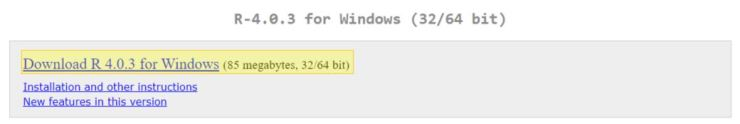
\includegraphics{data/03.png}

\begin{enumerate}
\def\labelenumi{\arabic{enumi}.}
\setcounter{enumi}{4}
\item
  El archivo instalador empieza a descargarse como cualquier otro documento, la ubicación de la descarga y la forma en que se realice dependerán de la configuración que estés usando en tu navegador de internet.
\item
  Una vez que la descarga se complete, ejecuta el archivo de instalación desde la carpeta donde se haya almacenado.
\item
  Selecciona el idioma de preferencia y presiona OK.
\end{enumerate}

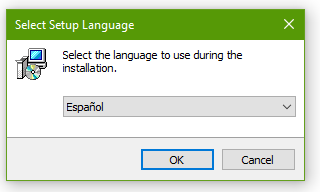
\includegraphics{data/04.png}

\begin{enumerate}
\def\labelenumi{\arabic{enumi}.}
\setcounter{enumi}{7}
\tightlist
\item
  Sigue las recomendaciones de la pantalla y luego presiona ``Siguiente''.
\end{enumerate}

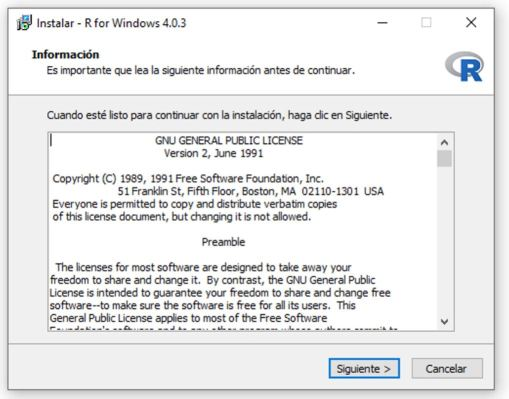
\includegraphics{data/08.png}

\begin{enumerate}
\def\labelenumi{\arabic{enumi}.}
\setcounter{enumi}{8}
\tightlist
\item
  Selecciona la carpeta donde quieres instalar R. La recomendación es dejar la carpeta que viene por defecto. Luego, presiona ``Siguiente''.
\end{enumerate}

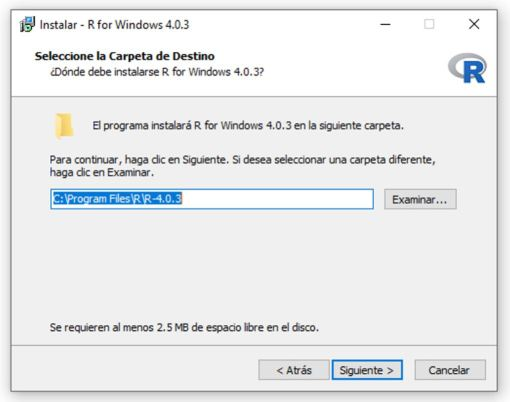
\includegraphics{data/09.png}

\begin{enumerate}
\def\labelenumi{\arabic{enumi}.}
\setcounter{enumi}{9}
\tightlist
\item
  Selecciona los componentes que desea instalar. Es recomendable dejar seleccionados los que vienen por defecto. Luego, presiona ``Siguiente''.
\end{enumerate}

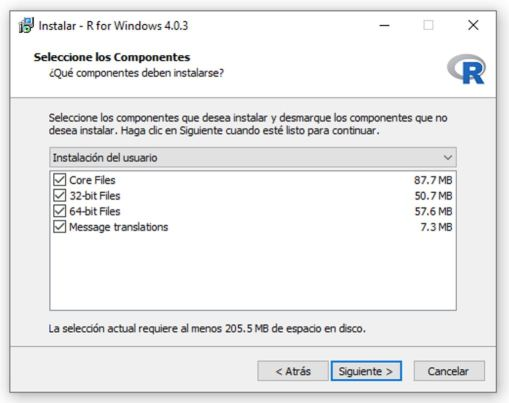
\includegraphics{data/10.png}

\begin{enumerate}
\def\labelenumi{\arabic{enumi}.}
\setcounter{enumi}{10}
\tightlist
\item
  Especifica las opciones de configuración. En este caso, como es la instalación básica, la opción sugerida es ``No''. Luego, presiona ``Siguiente''.
\end{enumerate}

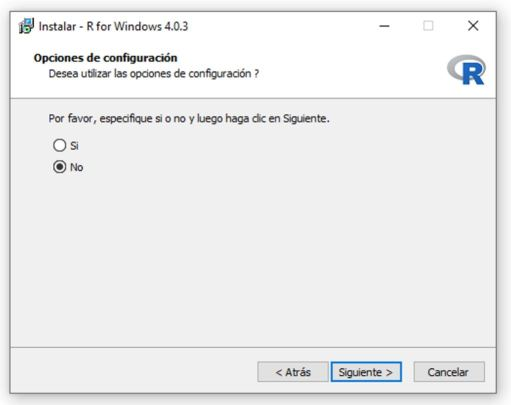
\includegraphics{data/11.png}

\begin{enumerate}
\def\labelenumi{\arabic{enumi}.}
\setcounter{enumi}{11}
\tightlist
\item
  Lee las indicaciones y selecciona las opciones de su conveniencia. La sugerencia es dejar las opciones que vienen por defecto. Luego, presiona ``Siguiente''.
\end{enumerate}

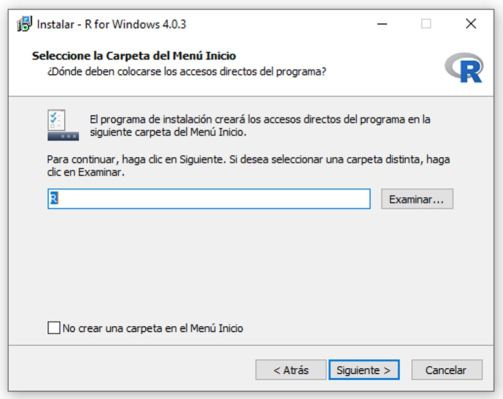
\includegraphics{data/12.png}

\begin{enumerate}
\def\labelenumi{\arabic{enumi}.}
\setcounter{enumi}{12}
\tightlist
\item
  Selecciona las tareas adicionales. La sugerencia es dejar habilitadas solamente las que vienen por defecto. Luego, presiona ``Siguiente''.
\end{enumerate}

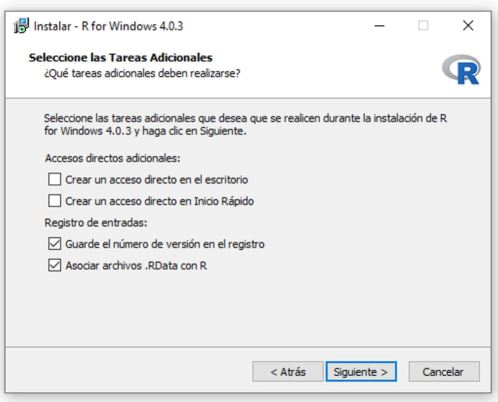
\includegraphics{data/13.png}

\begin{enumerate}
\def\labelenumi{\arabic{enumi}.}
\setcounter{enumi}{13}
\tightlist
\item
  Esto iniciará el proceso de instalación. No cierres la ventana hasta que el programa indique que el proceso ha sido completado con éxito.
\end{enumerate}

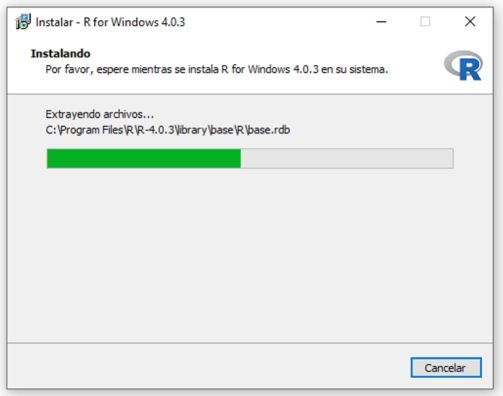
\includegraphics{data/14.png}

\begin{enumerate}
\def\labelenumi{\arabic{enumi}.}
\setcounter{enumi}{14}
\tightlist
\item
  Esto completa la instalación de R. Presiona ``Finalizar''.
\end{enumerate}


\includegraphics{data/15.png}

\hypertarget{instalaciuxf3n-de-r-studio-en-windows}{%
\subsection{Instalación de R Studio en Windows}\label{instalaciuxf3n-de-r-studio-en-windows}}

Vamos ahora a proceder con R Studio.

\begin{enumerate}
\def\labelenumi{\arabic{enumi}.}
\item
  Abre el siguiente enlace \url{https://R} Studio.com/products/R Studio/download/\#download
\item
  En esta página, se indica lo siguiente:
\end{enumerate}

2.1. Install R: Se requiere que R esté preinstalado. La versión más antigua soportada es 3.0.1, si se siguieron los pasos descritos anteriormente para la instalación de R tendríamos la versión más nueva, por lo que no tendríamos problema.

2.2. Download R Studio Desktop: R Studio provee un instalador sugerido basado en su sistema. En la imagen de abajo el instalador sugerido es Windows porque es el sistema operativo detectado. Si el instalador coincide con su sistema operativo, haga click en el recuadro para iniciar la descarga. Si requiere otro instalador, mirar el punto 3.

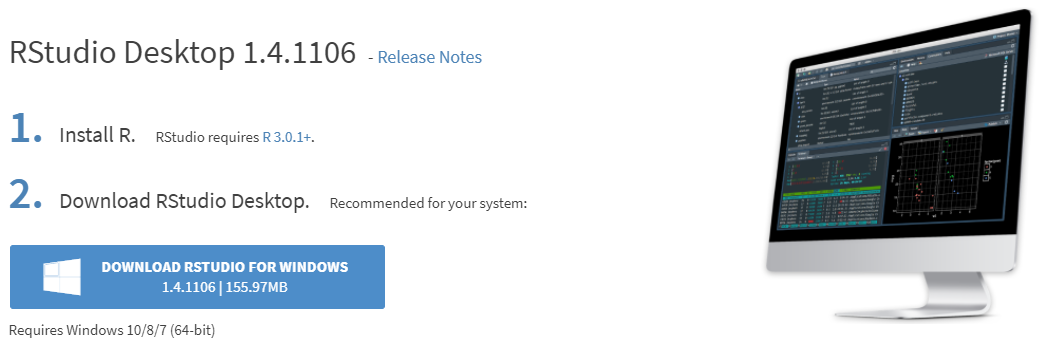
\includegraphics{data/R01.png}

\begin{enumerate}
\def\labelenumi{\arabic{enumi}.}
\setcounter{enumi}{2}
\tightlist
\item
  En caso de requerir instaladores para otros sistemas operativos, estos se pueden encontrar en el cuadro abajo de la imagen en la misma página ``All Installers''.
\end{enumerate}

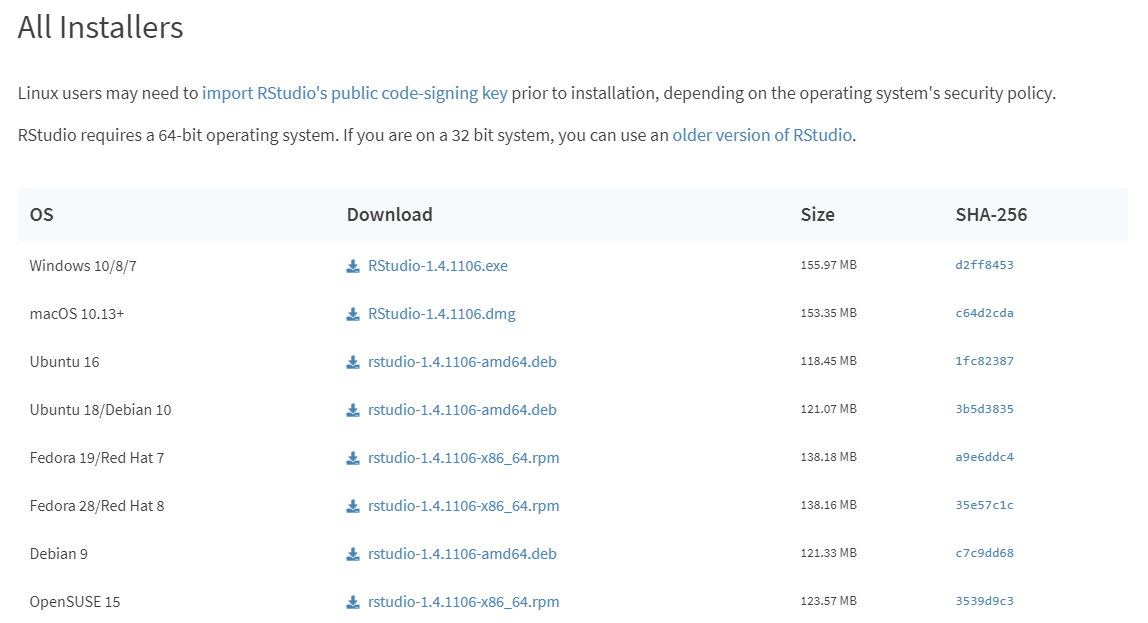
\includegraphics{data/R02.png}

\begin{enumerate}
\def\labelenumi{\arabic{enumi}.}
\setcounter{enumi}{3}
\item
  Después de seleccionar la descarga del instalador correspondiente, el archivo empezará a descargarse como cualquier otro documento, la ubicación de la descarga y la forma en que se realice dependerán de la configuración que estés usando tu navegador de internet.
\item
  Una vez que la descarga se complete, ejecuta el archivo de instalación desde la carpeta donde haya sido descargado.
\item
  La ventana de bienvenida indica que es recomendado cerrar todas las demás aplicaciones que se estén usando antes de iniciar la instalación. Esto es para que sea posible actualizar archivos importantes en el sistema sin necesidad de reiniciar el PC. Presiona ``Next'' cuando se haya completado lo anterior o si no hay inconveniente con reiniciar el PC.
\end{enumerate}


\includegraphics{data/R06.png}

\begin{enumerate}
\def\labelenumi{\arabic{enumi}.}
\setcounter{enumi}{6}
\tightlist
\item
  Seleccion la carpeta donde instalar R Studio. La recomendación es dejar la carpeta que viene por defecto. Luego, presiona ``Next''.
\end{enumerate}

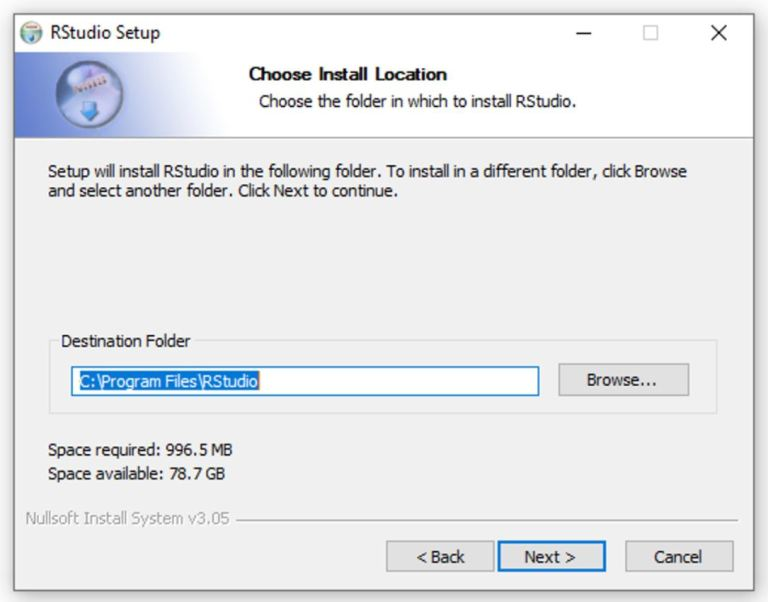
\includegraphics{data/R07.png}

\begin{enumerate}
\def\labelenumi{\arabic{enumi}.}
\setcounter{enumi}{7}
\tightlist
\item
  Selecciona la carpeta del menú de Inicio en el que se crearán los accesos directos al programa, o escribe un nombre para crear una nueva carpeta. La sugerencia es dejar las opciones que vienen por defecto. Luego, presiona ``Install''.
\end{enumerate}

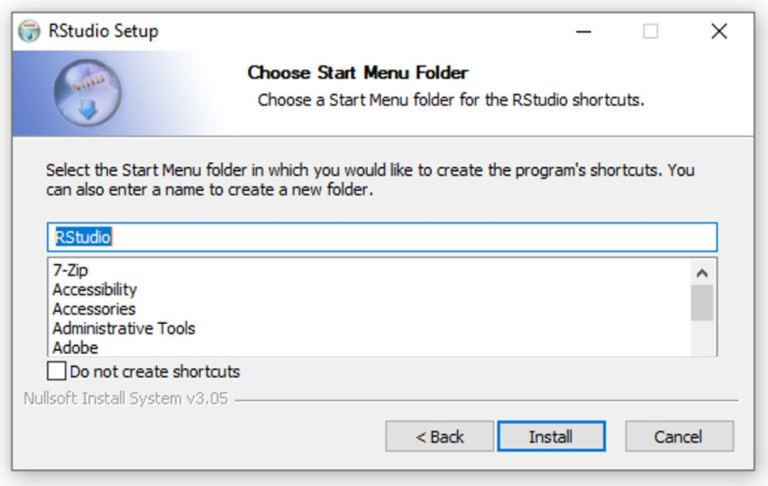
\includegraphics{data/R08.png}

\begin{enumerate}
\def\labelenumi{\arabic{enumi}.}
\setcounter{enumi}{8}
\tightlist
\item
  Esto iniciará el proceso de instalación. No cierres la ventana hasta que el programa indique que el proceso ha sido completado con éxito.
\end{enumerate}

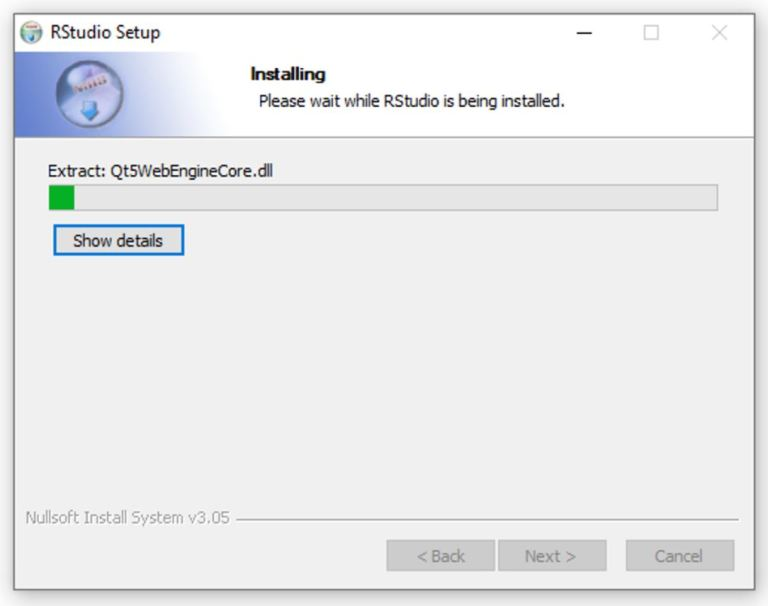
\includegraphics{data/R09.png}

\begin{enumerate}
\def\labelenumi{\arabic{enumi}.}
\setcounter{enumi}{9}
\tightlist
\item
  Esto completa la instalación de R Studio. Presiona ``Finalizar''; es posible que debas reiniciar el PC dependiendo de lo establecido en el paso 6.
\end{enumerate}


\includegraphics{data/R10.png}

\begin{enumerate}
\def\labelenumi{\arabic{enumi}.}
\setcounter{enumi}{10}
\tightlist
\item
  Tras el posible reinicio o sin el reinicio, lanza R Studio como cuqlquier otra aplicación. este es su aspecto.
\end{enumerate}

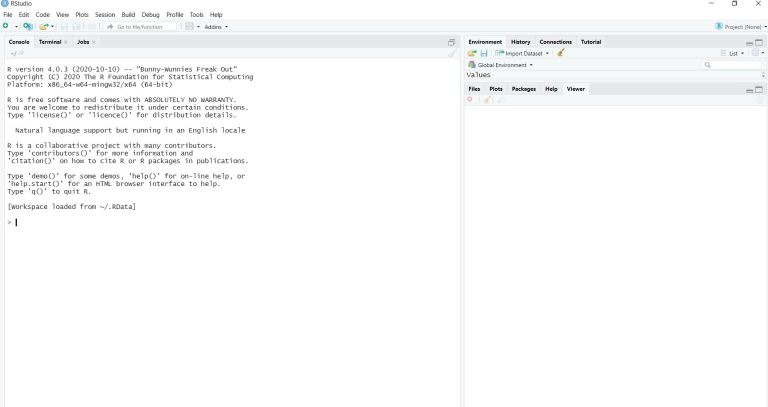
\includegraphics{data/R11.png}

A partir de aquí continuamos. R Studio se encarga de gestionar R, no deberemos preocuparnos por éste salvo para actualizarlo cuando creamos necesario o tengamos alguna necesidad puntual. R y R Studio son como cualquier otra aplicación de Windows, harás lo mismo que con las demás.

\hypertarget{uso-buxe1sico-de-r-studio-y-de-r}{%
\section{Uso básico de R Studio y de R}\label{uso-buxe1sico-de-r-studio-y-de-r}}

Si eres un lector / usuario que ya ha trabajado con R y R Studio, puedes saltar ya lo que resta de sección y pasar directamente a la sección 3. Si no lo eres, unas breves instrucciones para comenzar.

\hypertarget{quuxe9-es-r-studio-una-interfaz-para-usar-r}{%
\subsection{¿Qué es R Studio?: una interfaz para usar R}\label{quuxe9-es-r-studio-una-interfaz-para-usar-r}}

Cuando arrancamos R Studio, se pueden ver 4 ventanas, que según el gusto del usuario, pueden estar organizadas de diversa forma. En mi caso, me gusta disponer del editor de scripts o sintaxis ( \emph{source} ) en la parte superior izquierda, en la parte superior derecha la consola ( \emph{console} ) y abajo de izquierda a derecha el entorno ( \emph{environment} ) y a la derecha el resto de opciones ( \emph{files}, \emph{plots}, \ldots) en la parte superior el además de la barra de opciones en la parte superior.

Puedes adoptar esta configuración desde el menú \textbf{\emph{Tools \textgreater{} Global Options \textgreater{} Pane Layout}}.

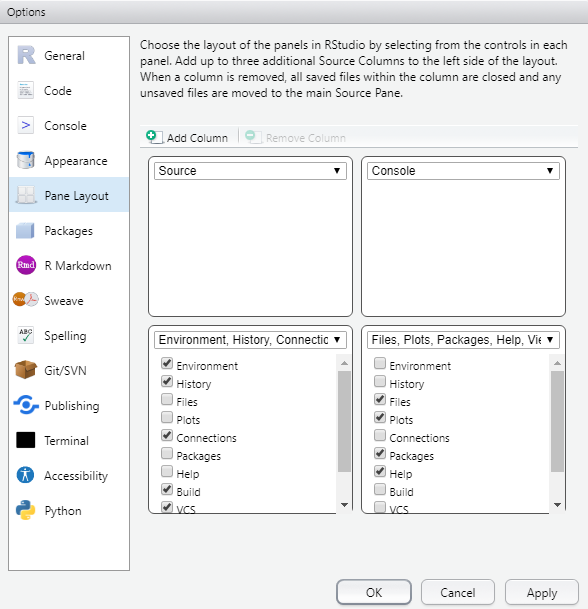
\includegraphics{data/RS01.png} Mi escritorio \ldots{}

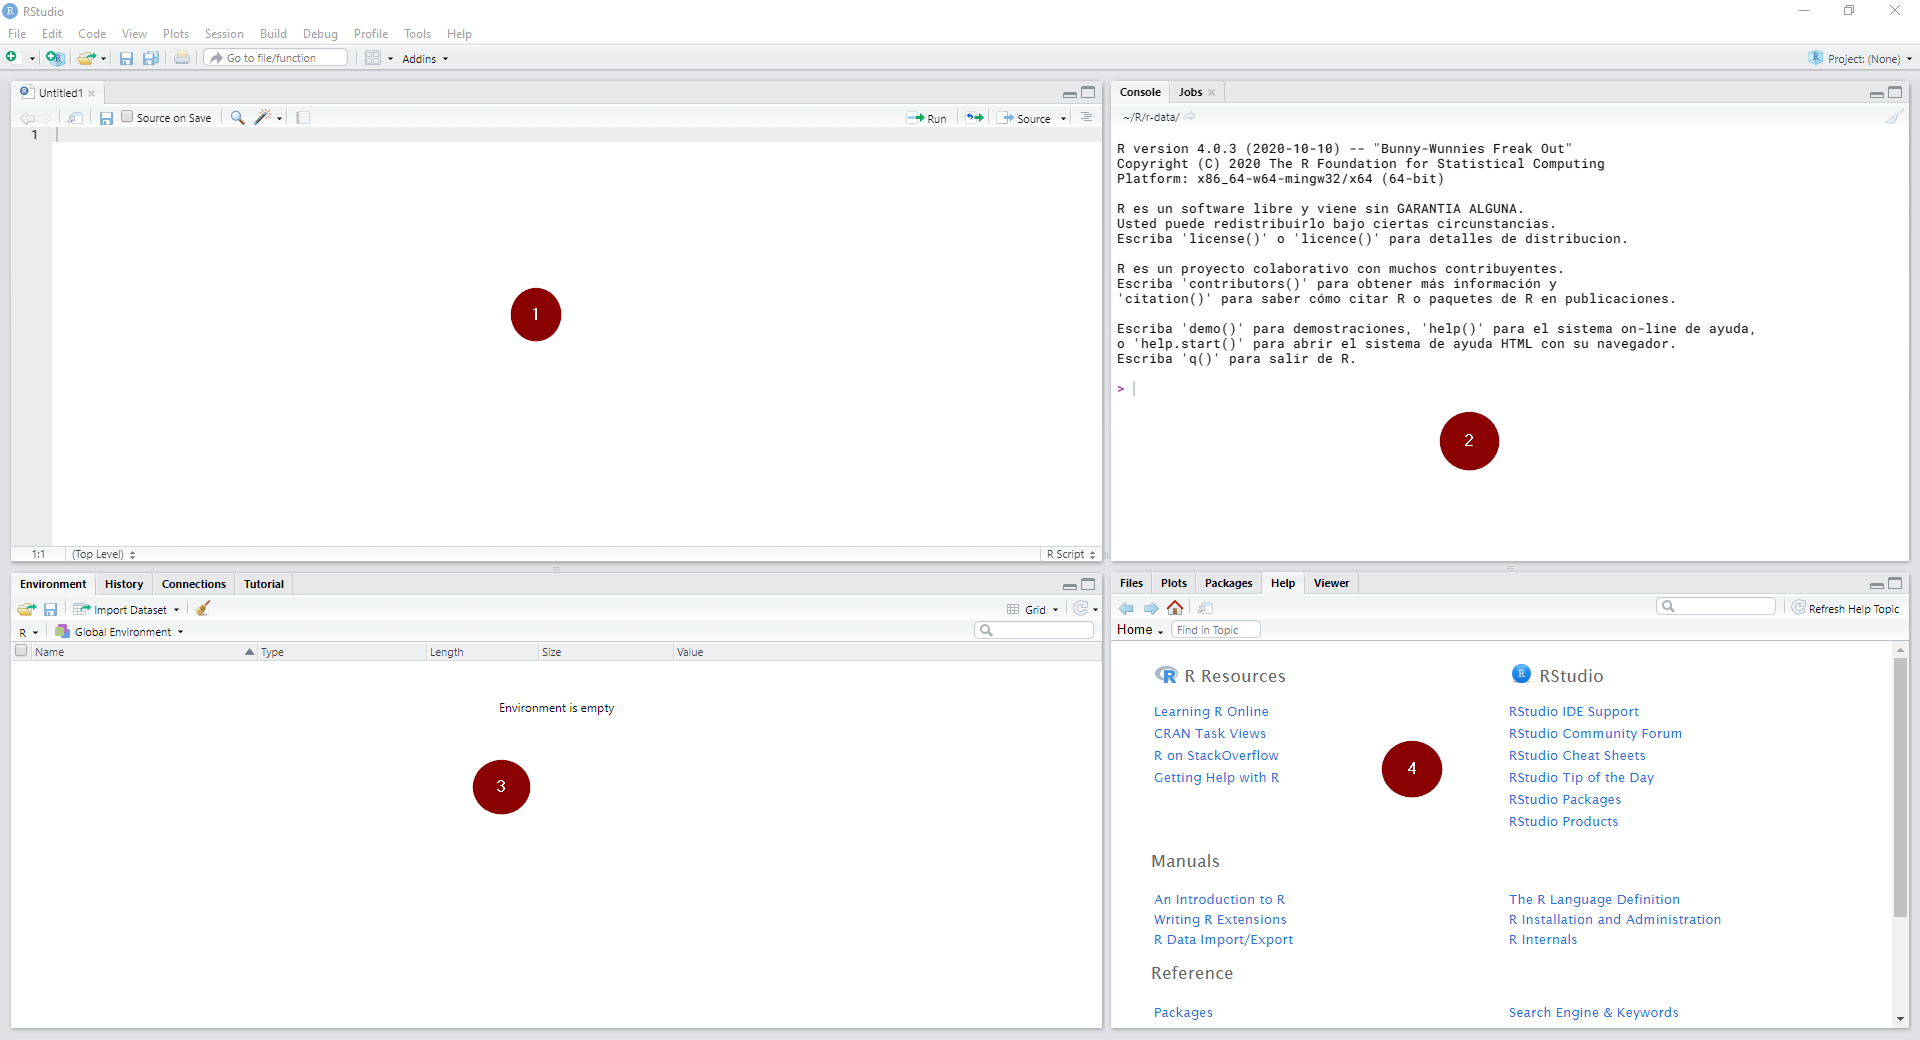
\includegraphics{data/RS03.png}

Ventana (1): es el editor de sintaxis: se trata del lugar donde editamos la sintaxis para posteriormente ejecutarla. Al escribir allí no sucederá nada, a no ser que se apriete algún botón para ejecutar los comandos o la tecla CTRL+ENTER.

Ventana (2): es la consola. Corresponde a lo que sería el software R en su versión básica. Allí el software ejecuta las operaciones realizadas desde el editor de sintaxis.

Ventana (4): es el ``entorno de trabajo'' del programa: en este lugar se muestra el conjunto de datos y los ``objetos'' (resultados, variables, gráficos, etc.) que se almacenan al ejecutar diferentes análisis.

Ventana (4) tiene varias sub pestañas: (i) la pestaña files permite ver el historial de archivos trabajados con el programa; (ii) la pestaña plots permite visualizar los gráficos que se generen; (iii) la pestaña packages permite ver los paquetes descargados y guardados en el disco duro así como gestionar su instalación o actualización; (iv) la ventana help permite acceder al CRAN - Comprehensive R Archive Network (siempre que se cuente con conexión a Internet), página oficial del software que ofrece diferentes recursos para el programa: manuales para el usuario, cursos on line, información general, descarga de paquetes, información de los paquetes instalados, etc. Esta última pestaña es bastante útil: empleando el motor de búsqueda se accede de manera rápida a manuales de uso de los diferentes paquetes (y sus funciones) instalados en el computador (esto no requiere conexión a Internet).7; (v) la ventana viewer muestra los resultados al construir reportes mediante funcionalidades tipo R Markdown que será nuestra herramienta de trabajo.

¿Dónde está nuestro trabajo? El software R funciona como un entorno temporal de trabajo, esto quiere decir que el usuario va agregando datos y objetos (conjuntos de datos con diferentes atributos) a una ``hoja en blanco''. Hay que tener en cuenta que R trabaja con la memoria activa (RAM) del computador, por lo tanto cualquier análisis sólo mostrará la información resultante pero no permanecerá como archivo posible de utilizar de modo posterior. Es decir, si los análisis no son guardados como objetos (vectores, matrices, listas u otros tipos de objetos) se deberán repetir las instrucciones para obtener otra vez el resultado.

Todas las operaciones de R - sean indicadas vía sintaxis o botones - son ejecutadas según comando computacional que es visualizado en la consola. La ejecución de comandos entrega diferentes señales respecto a su funcionamiento. Por ejemplo, mientras se está ejecutando un comando, el programa muestra un signo ``Stop'' en la esquina superior derecha de la consola (como se ve en la imagen). Eso indica que el programa está ocupado ejecutando una acción. Si se presiona tal símbolo, se cancelará la operación en curso.

En la sección \ref{tse02}, comenzamos a trabar con sccripts que nos devuelvan resultados.

\hypertarget{tse02}{%
\chapter{Primeros pasos y términos a conocer}\label{tse02}}

\hypertarget{desde-duxf3nde-creo-mis-scripts}{%
\section{¿Desde dónde creo mis scripts?}\label{desde-duxf3nde-creo-mis-scripts}}

Dos son las formas de trabajar con R desde R Studio. Te explicamos brevemente esas dos formas de trabajar.

\hypertarget{scripts-en-consola}{%
\subsection{Scripts en consola}\label{scripts-en-consola}}

El scripting con consola está pensado para obtener tablas u otros objetos en la consola de la interfaz de trabajo de R Studio. Para ello usaremos archivos de texto con extensión .R que crearemos desde la entrada \emph{File \textgreater{} New File \textgreater{} R Script}. Estos ficheros darán como resultado salidas a la denominada consola en formato de texto.

\hypertarget{scripting-con-markdown}{%
\subsection{\texorpdfstring{Scripting con \emph{markdown}}{Scripting con markdown}}\label{scripting-con-markdown}}

El scripting con \emph{markdown} está pensado para generar páginas completas o documentos completos con texto, tablas, gráficos, etc. Se pueden utilizar paquetes como \texttt{flexdashboard} o generar salidas de tipo diapositiva utilizando las opciones de configuración que ofrece el paquete \texttt{rmarkdown}. No aseguramos una compatibilidad al 100\%, pues eso sería imposible, pero gran parte de las características estarían funcionales. La idea es generar un documento HTML, de forma totalmente transparente para el usuario, que se guarda en la base de datos y se presenta como resultado del análisis. Ese HTML puede contener texto, gráficos, tablas y cualquier elemento que se te ocurra. El código R se ubica en lo que se denomina \texttt{chunk} -que luego veremos- y se puede incluir también código R \texttt{inline} en el texto. Para esta segunda forma de trabajar usaremos también archivos de texto, pero con extensión .Rmd que crearemos desde la entrada \emph{File \textgreater{} New File \textgreater{} R Markdown}. Estos ficheros darán como resultado archivos con extensiones .html, .docx, .pdf.

\hypertarget{primeros-pasos}{%
\section{Primeros pasos}\label{primeros-pasos}}

Si ya tienes experiencia con R Studio, da un vistazo, pero es posible que mucho de lo aquí indicado sea irrelevante para ti y todo ello ya sea habitual y conocido por ti. Pasa a la siguiente sección, donde comenzamos a trabajar los scripts.

\hypertarget{carga-de-datos}{%
\subsection{Carga de datos}\label{carga-de-datos}}

Vamos a trabajar con ello y verás que sencillo. Para comenzar, en \href{https://drive.google.com/uc?export=download\&id=1JjevbQjzGc1NMyR7qf7bbvtbMyK8Pvhr}{este enlace} tienes un archivo de datos con el que haremos todos nuestros ejemplos. Esta fuente de datos está en formato SPSS (*.sav) y se corresponde con la tercera oleada de un estudio del CIS (Centro de Investigaciones Sociológics de España) de 2017, el barómetro sanitario.
La fuente de datos tiene 2557 registros y tiene 190 campos. Si deseas ver el cuestionario que originalmente se utilizó para recoger los datos, \href{https://drive.google.com/uc?export=download\&id=1AUUI-1isOmKB1ovR4MRoqMj2Fp7Re2f2}{lo puedes descargar aquí}. En él puedes ver todo lo referente a como se ha realizado la entrevista.

Si has seguido las instrucciones de instalación, se habrá creado una carpeta denominada R dentro de Mis Documentos (que R Studio denomina Home como podás observar en el panel de la ventana 4, opción FILES)

A partir de ahí,impera tu orden, agrega carpetas en la forma en que esté habituado y organiza tu trabajo como si de cualquier aplicación Windows se tratara. Si te gusta ser ordenado en tu trabajo, lo harás también; si no te gusta, \ldots{}

Nuestro primer paso será iniciar una sintaxis o script. Para ello desde el menú de \textbf{\emph{File \textgreater{} New File \textgreater{} R Script}} abriremos un espacio para escribir. En la ventana creada como \emph{Untitled1}, puedes escribir.

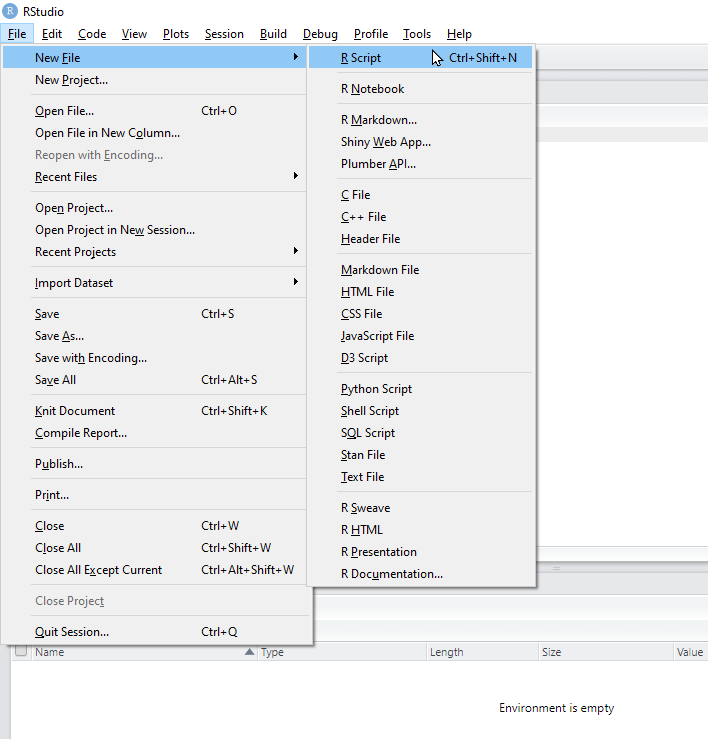
\includegraphics{data/RS04.png}

escribe 2+2 y haz clic en \emph{Run} teniendo el cursor sobre la línea en la que has escrito \ldots{}

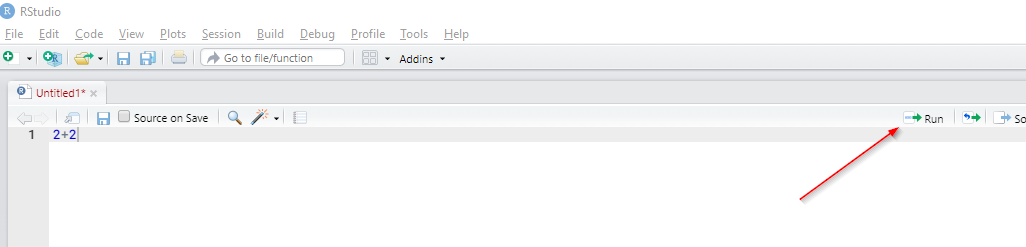
\includegraphics{data/RS05.png}

y obtendrás el resultado en la consola (ventana 2)

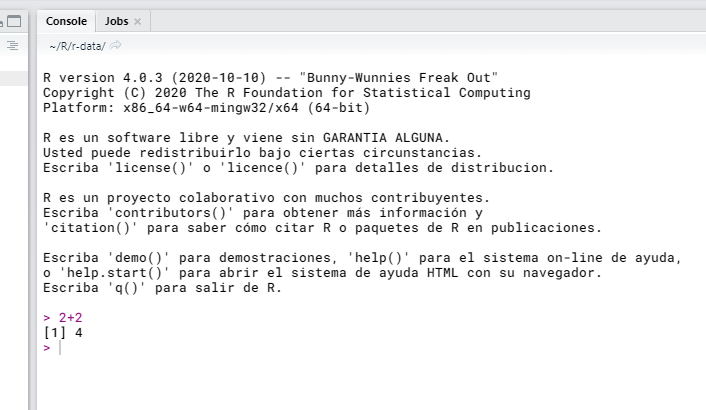
\includegraphics{data/RS06.png}

Ahora podrías guardar tu script \emph{File \textgreater{} Save as} , y ya tendríamos cerrado el primer paso del camino. El archivo puede abrirse, ser editado y volver a ejecutarse tantas veces quieras.

\hypertarget{instalaciuxf3n-de-paquetes}{%
\subsection{Instalación de paquetes}\label{instalaciuxf3n-de-paquetes}}

Uno de los elementos fundamentales que caracteriza a R, es que se trabaja con \textbf{paquetes} que la comunidad de desarrollo aporta para los análisis más variados. Los paquetes son la aportación de los desarrolladores que de alguna forma comparten su conocimiento con la comunidad global. Nosotros vamos a trabajar con algunos que no están en la instalación base, asi que procederemos a hacer el ciclo completo de instalación (sólo una vez) y carga (tantas veces como queramos usar el paquete en una sesión). Aunque existe opción de instalar paquetes por comandos \texttt{install.packages()}, ilustramos el camino para hacerlo desde el menú. \textbf{\emph{Tools \textgreater{} Install packages}}.

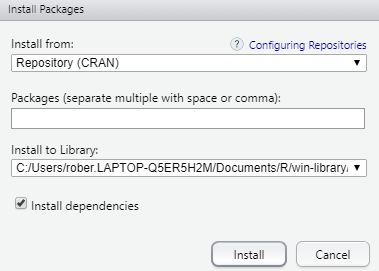
\includegraphics{data/install_packages.png}

Utiliza la opción arriba indicada y siguiendo las indicaciones descritas escribiríamos:

\textbf{expss, highcharter, kableExtra}

Cuando hagas clic en \emph{Install}, comenzarán a instalarse esos paquetes (su descarga e instalación). R Studio te informa cuando ha finalizado. Puede verse en la consola.

\hypertarget{crear-un-fichero-r-markdown}{%
\section{Crear un fichero R Markdown}\label{crear-un-fichero-r-markdown}}

Vamos a crear un nuevo script, pero ahora ya lo vamos a hacer del modo que seguiremos trabajando durante todo el manual.

Desde el menú de R Studio \textbf{\emph{Files \textgreater{} New File \textgreater{} R Markdown}}. Elige entre las opciones proporcionadas, la creación de un \emph{documento HTML}. Dale nombre y ponte como autor. Verás lo que escribas reflejado en el archivo.

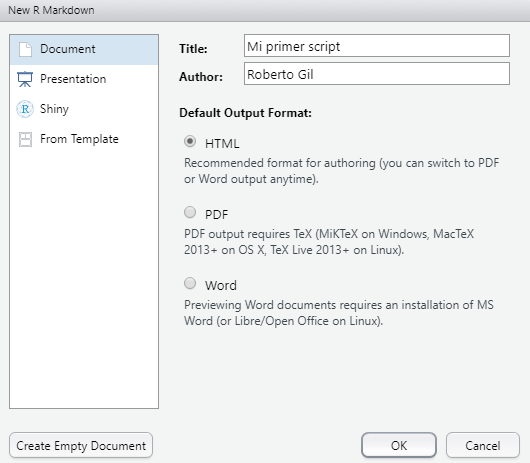
\includegraphics{data/RS07.png}

Se creará un archivo como este \ldots{}

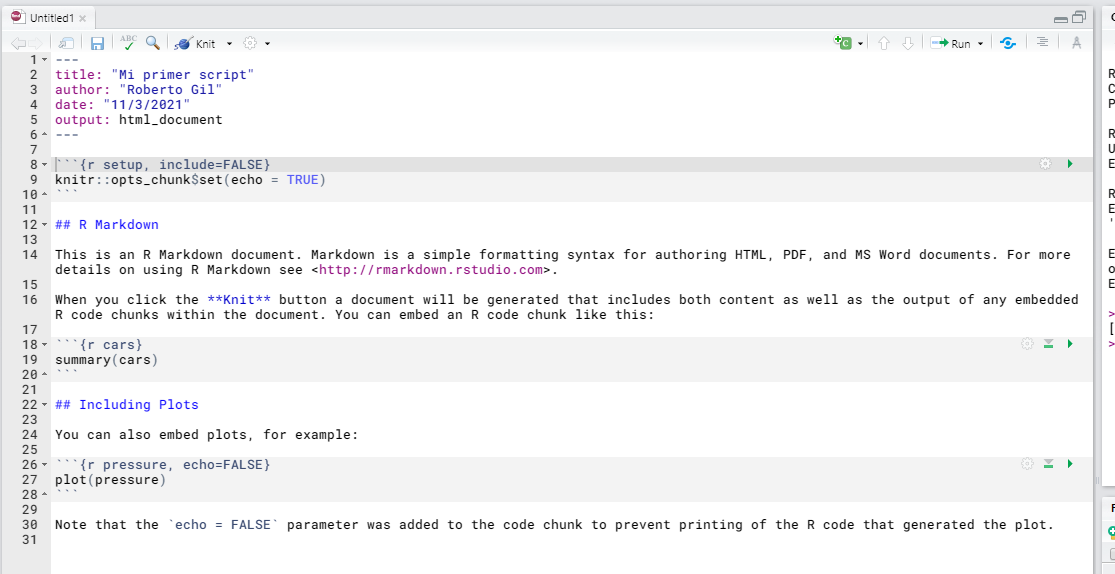
\includegraphics{data/RS08.png}
Este es un fichero de ejemplo, borra desde donde pone \#\# R Markdown hasta abajo y que quede así. Mantenemos este primer \emph{chunk} y lo explicamos.

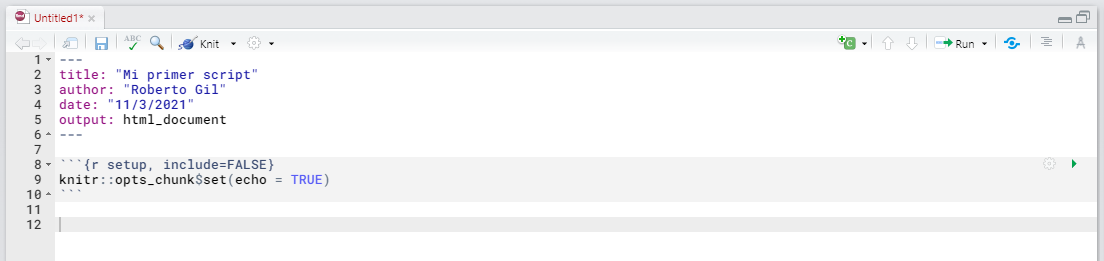
\includegraphics{data/RS09.png}

Aquí escribimos el script de R, que como puedes ver en línea 1 y 3 comienza y acaba con una simbología determinada. Estos son los caracteres indicadores de que todo lo que queda entre \texttt{\textasciigrave{}\textasciigrave{}\textasciigrave{}\{r\ echo\ =\ TRUE\}} y \texttt{\textasciigrave{}\textasciigrave{}\textasciigrave{}} es scripting. A partir de ahora, nuestras instrucciones irán siempre entre estos símbolos de inicio y final. Nótese que se añade la instrucción \texttt{echo\ =\ TRUE}. Esta instrucción provocará que se imprima en el resultado los comandos del script, si en lugar de eso se escribe \texttt{echo=FALSE}, no se imprimiría ese código.

Nuestro código le dirá a R que secuencialmente haga\ldots{}

\begin{itemize}
\tightlist
\item
  la carga del paquete expss;
\item
  la lectura del archivo que está en esa URL (un archivo SAV - SPSS en Google Drive) y asignació a un objeto de R que lo contendrá llamado \emph{data};
\item
  el cálculo de la media (mean)\ldots;
\item
  de una variable que está en el marco de datos denominado \texttt{data};
\item
  y que se llama PESO (\texttt{data\$PESO});
\item
  no teniendo en cuenta los valores NA (nulos, no definidos, que no sean número: \texttt{na.rm=TRUE})
\end{itemize}

\begin{Shaded}
\begin{Highlighting}[]
\FunctionTok{suppressMessages}\NormalTok{(}\FunctionTok{setwd}\NormalTok{(}\StringTok{"\textasciitilde{}/R/r{-}projects/00.tables"}\NormalTok{))  }\CommentTok{\#esta es la carpeta donde almacené el archivo (en una subcarpeta llamada data)}
\FunctionTok{suppressMessages}\NormalTok{(}\FunctionTok{library}\NormalTok{(expss))  }\CommentTok{\#cargamos el paquete}
\FunctionTok{suppressMessages}\NormalTok{(data }\OtherTok{\textless{}{-}} \FunctionTok{read\_spss}\NormalTok{(}\StringTok{"data/3192.sav"}\NormalTok{))  }\CommentTok{\#cargamos los datos}
\FunctionTok{mean}\NormalTok{(data}\SpecialCharTok{$}\NormalTok{PESO, }\AttributeTok{na.rm =} \ConstantTok{TRUE}\NormalTok{)}
\end{Highlighting}
\end{Shaded}

\begin{verbatim}
## [1] 0.9999273
\end{verbatim}

Quedará así:

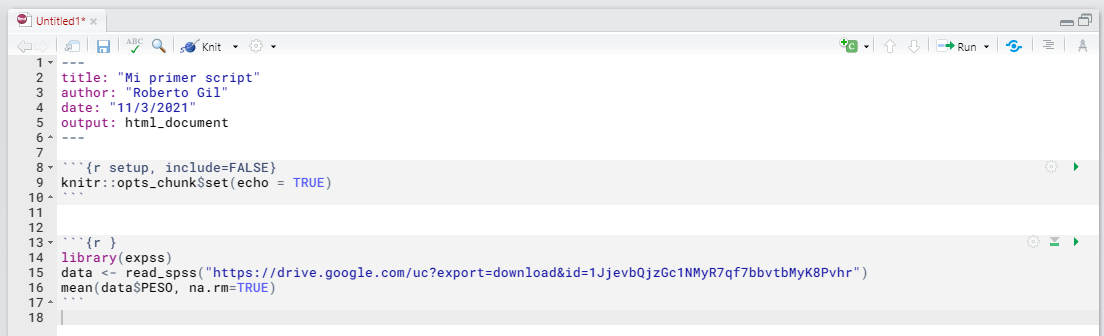
\includegraphics{data/RS10.png}

Para ver el resultado, haz clic en el botón \emph{\texttt{knitr}} (publicar). Como es la primera vez y no hemos guardado nuestro script, nos indica que le pongamos nombre, por ejemplo SCRIPT\_001.

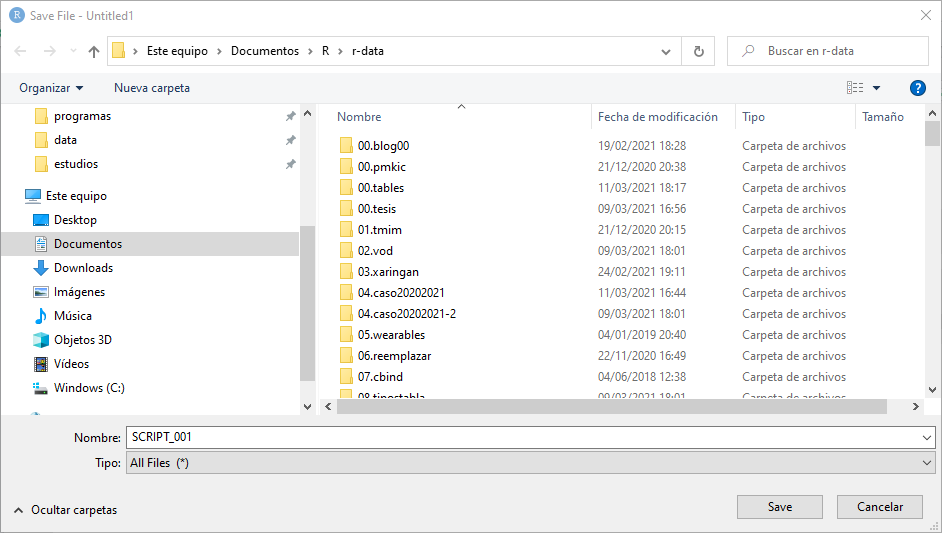
\includegraphics{data/RS11.png}

Y el resultado, ya puedes verlo, 0,9999273; sale en una nueva ventana que es donde se muestra el resultado. Reconocerás también aquello que se ha escrito cuando creamos el archivo y que puede editar sobre el fichero.

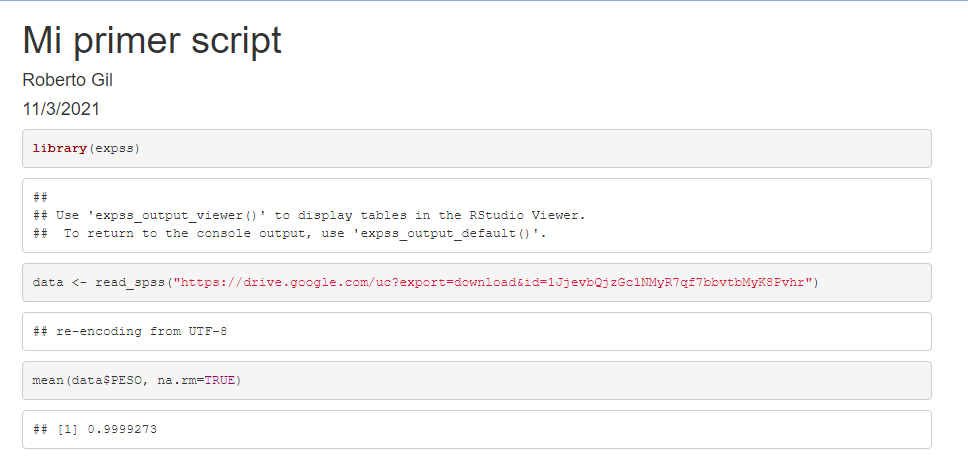
\includegraphics{data/RS12.png}

Fíjate que se ha publicado el código R de programación eso lo podemos evitar si cambiamos el \texttt{echo\ =\ TRUE} por \texttt{echo\ =\ FALSE}. Prueba a hacer el cambio y haz de nuevo \emph{\texttt{knitr}}.

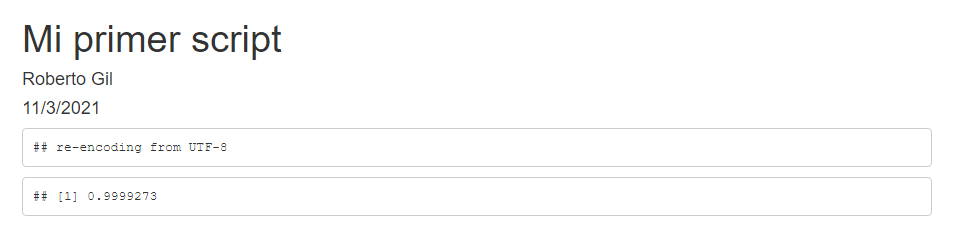
\includegraphics{data/RS13.png}

Terminamos con el primer script de análisis. Este script aparece ahora en el listado de fichero como SCRIPT\_001.Rmd (Rmd es la extensión de los archivos R Markdown, mientras que R es la de los scripts de consola). Del mismo modo, podrás ver ahora un archivo denominado SCRIPT\_001.html que contiene tu resultado y que podrías copiar o enviar a cualquiera porque contiene todo lo necesario para que se muestre como a ti. Una de las grandes ventajas.

\hypertarget{conclusiuxf3n}{%
\subsection{Conclusión}\label{conclusiuxf3n}}

Así, hemos finalizado con nuestro primer \emph{scripting}. No volveremos a ser tan explicativos en este documento acerca de como crear y editar los scripts. En la siguiente sección comenzamos con las tablas más básicas.

\hypertarget{buxe1sicos-de-r-yo-proceso-de-datos}{%
\section{Básicos de R y/o proceso de datos}\label{buxe1sicos-de-r-yo-proceso-de-datos}}

En el presente epígrafe, mostramos un conjunto de términos que serán habitualmente utilizados en las sucesivas secciones que se presentan en este documento. Estos son los más relevantes y los hemos separado en dos grupos. Un grupo hace referencia a términos básicos de R y otro grupo a términos básicos del manejo de tablas o del proceso de tabulación. Cada término tiene une breve reseña, y posteriormente algunos de ellos serán más tratados en sus respectivas funcionalidades.

\begin{enumerate}
\def\labelenumi{\arabic{enumi}.}
\item
  \textbf{R} es un entorno y lenguaje de programación con un enfoque al análisis estadístico. Nació como una implementación de software libre del lenguaje S, adicionado con soporte para alcance estático. Se trata de uno de los lenguajes de programación más utilizados en investigación científica, siendo además muy popular en los campos de aprendizaje automático o \emph{machine learning}, minería de datos, investigación biomédica, bioinformática y matemáticas financieras. A esto contribuye la posibilidad de cargar diferentes bibliotecas o paquetes con funcionalidades de cálculo y graficación. R es parte del sistema GNU y se distribuye bajo la licencia GNU GPL. Está disponible para los sistemas operativos Windows, Macintosh, Unix y GNU/Linux.
\item
  \textbf{objeto}, elemento creado desde comandos o scripts de R y que puede ser reutilizado dentro de la programación del script. En este manual se usará como sinónimo de tabla en muchos casos, pues la mayoría de los objetos que crearemos serán tablas.
\item
  \textbf{\emph{dataframe}}, fichero de datos, banco de datos; término con el que se conoce en R a la estructura tabular (filas y columnas) de una matriz de datos, donde las columnas son variables y las filas son registros.
\item
  \textbf{variable}, elemento de tipo vector que contiene los valores de una determinada observación, un valor en cada fila; debe entenderse en el contexto de la estructura tabular o \emph{dataframe}.
\item
  \textbf{valores}, cada una de las diferentes celdas que componen un \emph{dataframe}. Una variable toma un valor en cada fila y se representa en la celda.
\item
  \textbf{medidas}, valores de los que se pretende calcular estadísticos como la media, la desviación típica o la mediana entre otras. Suelen responder a escalas de tipo numérico (ordinal o métrico).
\item
  \textbf{dimensiones}, valores de los que se pretende calcular frecuencias y/o porcentajes.
\item
  \textbf{factores}, niveles, códigos, etiquetas de variable.
\item
  \textbf{NA}, es como R representa los valores nulos o ausentes.
\item
  \textbf{valores} perdidos, \emph{missing values}, valores ausentes; tal como hemos indicado en el término NA, así es como R representa este tipo de valores.
\item
  \textbf{paquete}, conjunto de funciones de las que el usuario hace uso para obtener un resultado en R; en nuestro caso particular principalmente usaremos el paquete EXPSS de R; 1. comando, instrucciones que se integran dentro de un chunk
\item
  \textbf{chunk}, conjunto de comandos que se escriben entre los símbolos \texttt{\{r\}\ y} y que se ejecutan mostrando los resultados.
\end{enumerate}

\hypertarget{buxe1sicos-de-tabulaciuxf3n}{%
\section{Básicos de tabulación}\label{buxe1sicos-de-tabulaciuxf3n}}

Antes de comenzar, el término más importante y objeto de nuestro trabajo.

\begin{quote}
Tabla
\end{quote}

Una tabla es una matriz o cuadro que muestra la relación entre (una) dos o más variables. Cuando la tabla solo muestra la relación entre dos variables de tipo nominal u ordinal, y también se conoce como tabla de contingencia \citep{sanchez1989analisis}.

En nuestro trabajo vamos a crear objetos de tipo tabla; una tabla es una estructura tabular, igual que un \emph{dataframe}. De hecho, con nuestro trabajo utilizando el paquete EXPSS, vamos a generar tablas que serán \emph{dataframe} de tipo (clase) \texttt{etable}. Al ser un \emph{dataframe}, podremos operar entre filas, columnas y celdas de forma lógica o aritmética utilizando funciones y comandos de R.

Además, dejamos este glosario de términos relacionados con las tablas en R, que utilizaremos en esta guía.

\begin{enumerate}
\def\labelenumi{\arabic{enumi}.}
\tightlist
\item
  \textbf{título} o \emph{caption}, texto que se publicará sobre la tabla;
\item
  \textbf{pie} o \emph{footer}, texto que se publicará bajo la tabla;
\item
  \textbf{fila}, cada una de las líneas de información dentro de una tabla; se suele asimilar a un nivel (código) de una variable y/o a un resultados estadístico de una variable;
\item
  \textbf{columna}, cada una de las variables que conforman el \emph{dataframe} de una tabla (estructura tabular); en un cuadro o tabla de contingencia suele equivaler a un nivel de la variable que originalmente se diseñó para ser usada en columnas (si por ejemplo SEXO, una columna sería hombre y otra mujer);
\item
  \textbf{celda}, cada una de las unidades de información del cuadro o tabla;
\item
  \textbf{row\_label}, primera columna donde se escriben los textos de las filas y que sirven para identificar el contenido de las mismas;
\item
  \textbf{etiqueta de variable}, texto extra identificativo de la variable usada en filas o columnas;
\item
  \textbf{etiqueta de valor}, texto del código identificativo de la variable usada;
\item
  \textbf{estadístico}, medida calculada;
\item
  \textbf{frecuencia}, tipo específico de medida calculada que significa número de veces en términos absolutos;
\item
  \textbf{porcentaje}, tipo específico de medida calculada que significa número de veces en términos relativos;
\item
  \textbf{\texttt{\textbar{}}}, símbolo denominado \texttt{pipe} que en el paquete \texttt{expss} se utilizará para separar conjuntos de texto en una celda (o columna o fila);
\item
  \textbf{significación}, prueba estadística de contraste.
\end{enumerate}

Hasta aquí esta introducción. En la sección \ref{tse03} avanzaremos en la realización de las tablas básicas o también llamadas univariantes o marginales.

\hypertarget{tse03}{%
\chapter{Tablas marginales}\label{tse03}}

\hypertarget{una-pequeuxf1a-introducciuxf3n}{%
\section{Una pequeña introducción}\label{una-pequeuxf1a-introducciuxf3n}}

Vamos a comenzar explicando un poco qué es \texttt{expss}y su similitud nominal con \texttt{IBM\ SPSS}. \texttt{expss} es un paquete desarrollado por \citet{expss} que calcula y muestra tablas de todo tipo, con soporte para etiquetas con estilo \texttt{SPSS} y con gran facilidad y flexibilidad para obtener cabeceras múltiples y anidadas, pesos, variables de respuesta múltiple y pruebas de significación de tabla y celda. Ofrece facilidades para una salida formateada de tablas, e incluso, aunque no es objeto de este manual la posibilidad de exportación de esas tablas a \texttt{EXCEL} con el paquete \texttt{openxlsx}. Los métodos para variables etiquetadas agregan soporte de etiquetas de valor a las funciones de R base y a algunas funciones de otros paquetes. Es un paquete destinado a ayudar a los analistas a cambiar el proceso de datos desde \texttt{EXCEL} y \texttt{SPSS} hasta R.

Aquí dejo algunos enlaces para que puedas leer acerca de este paquete y las posibilidades que te ofrece de modo combinado con R Studio:

\begin{itemize}
\tightlist
\item
  \href{https://cran.r-project.org/web/packages/expss/expss.pdf}{manual PDF de EXPSS}
\item
  \href{https://cran.r-project.org/web/packages/expss/vignettes/tables-with-labels.html}{material de ayuda, ejemplos}
\item
  \href{https://cran.r-project.org/web/packages/expss/vignettes/labels-support.html}{uso de etiquetas en R}
\end{itemize}

Vamos a crear nuestra primera tabla utilizando una instrucción muy básica de \texttt{expss}, que evolucionará en posteriores secciones. La que vas a ver seguidamente es la forma básica de pedir que se calcule la media de la variable PESO usando \texttt{expss}; le indicamos:

\begin{itemize}
\tightlist
\item
  la instrucción de cálculo \emph{calculate};
\item
  el marco de datos a usar, \emph{data};
\item
  y el cálculo a hacer \emph{cro\_mean} (equivalente a calcula la media \emph{mean}) en forma de tabla.
\end{itemize}

Así pues, crea un fichero R MarkDown como vimos en la sección \ref{tse02}, y escribe este código (o mejor \emph{copy\&paste}) y obtén el resultado \ldots{}

\begin{Shaded}
\begin{Highlighting}[]
\FunctionTok{setwd}\NormalTok{(}\StringTok{"\textasciitilde{}/R/r{-}projects/00.tables"}\NormalTok{)  }\CommentTok{\# esta es la carpeta donde almacené el archivo (en una subcarpeta llamada data)}
\FunctionTok{library}\NormalTok{(expss)  }\CommentTok{\#cargamos el paquete}
\NormalTok{data }\OtherTok{\textless{}{-}} \FunctionTok{read\_spss}\NormalTok{(}\StringTok{"data/3192.sav"}\NormalTok{)  }\CommentTok{\#cargamos los datos}
\end{Highlighting}
\end{Shaded}

\begin{verbatim}
## re-encoding from UTF-8
\end{verbatim}

\begin{Shaded}
\begin{Highlighting}[]
\FunctionTok{calculate}\NormalTok{(data, }\FunctionTok{cro\_mean}\NormalTok{(PESO))  }\CommentTok{\#hacemos el cálculo}
\end{Highlighting}
\end{Shaded}

 
  \providecommand{\huxb}[2]{\arrayrulecolor[RGB]{#1}\global\arrayrulewidth=#2pt}
  \providecommand{\huxvb}[2]{\color[RGB]{#1}\vrule width #2pt}
  \providecommand{\huxtpad}[1]{\rule{0pt}{#1}}
  \providecommand{\huxbpad}[1]{\rule[-#1]{0pt}{#1}}

\begin{table}[ht]
\begin{centerbox}
\begin{threeparttable}
\captionsetup{justification=centering,singlelinecheck=off}
\caption{\label{tab:unnamed-chunk-3} }
 \setlength{\tabcolsep}{0pt}
\begin{tabularx}{1\textwidth}{p{0.5\textwidth} p{0.5\textwidth}}


\hhline{}
\arrayrulecolor{black}

\multicolumn{1}{!{\huxvb{0, 0, 0}{0}}p{0.5\textwidth}!{\huxvb{0, 0, 0}{0}}}{\hspace{6pt}\parbox[b]{0.5\textwidth-6pt-6pt}{\huxtpad{6pt + 1em}\raggedright \huxbpad{6pt}}} &
\multicolumn{1}{p{0.5\textwidth}!{\huxvb{0, 0, 0}{0}}}{\hspace{6pt}\parbox[b]{0.5\textwidth-6pt-6pt}{\huxtpad{6pt + 1em}\raggedright \#Total\huxbpad{6pt}}} \tabularnewline[-0.5pt]


\hhline{}
\arrayrulecolor{black}

\multicolumn{1}{!{\huxvb{0, 0, 0}{0}}p{0.5\textwidth}!{\huxvb{0, 0, 0}{0}}}{\hspace{6pt}\parbox[b]{0.5\textwidth-6pt-6pt}{\huxtpad{6pt + 1em}\raggedright Ponderación\huxbpad{6pt}}} &
\multicolumn{1}{p{0.5\textwidth}!{\huxvb{0, 0, 0}{0}}}{\hspace{6pt}\parbox[b]{0.5\textwidth-6pt-6pt}{\huxtpad{6pt + 1em}\raggedleft 1\huxbpad{6pt}}} \tabularnewline[-0.5pt]


\hhline{}
\arrayrulecolor{black}
\end{tabularx}
\end{threeparttable}\par\end{centerbox}

\end{table}
 

Verás algunos cambios respecto a la salida anterior pues no hemos indicado cuántos decimales, ni que redondeo, ni le hemos dicho que no tenga en cuenta los valores especiales o nulos\ldots{} y ha respondido de forma correcta.

Ya vamos viendo que eso puede dar mucho juego, pero vamos a ir de forma ordenada y presentando poco a poco todos los tipos de tabla jugando con diferentes variables del banco de datos (¡¡¡ sí\ldots{} \emph{dataframe}!!!) que hemos cargado. Comenzaremos con la creación de tablas unidimensionales o conocidas como marginales, para luego continuar con las tablas cruzadas (sección @fig(tse04)), y entre medio, iremos incorporando medidas estadísticas.

Vamos a comenzar con un conjunto de tablas muy sencillas. En ellas representaremos los valores obtenidos del análisis de un campo extraído de nuestra fuente de datos de referencia, la tercera oleada del Barómetro Sanitario en España de 2017 del realizado y publicado por el CIS. Por ahora, trabajaremos sólo con la variable denominada P31 (sexo del entrevistado), variable medida en escala nominal, cuyas etiquetas (valores) son hombre (1) y mujer (2) y con la variable P3, escala de satisfacción (1-10) con el funcionamiento del sistema sanitario español, medida de 1 a 10. En nuestra fuente de datos tenemos 2557 casos (entrevistas realizadas). Puedes ver estas preguntas en el cuestionario PDF que puedes bajar en la sección @fig(tse02).

Utilizaremos un script, es decir una pocas líneas de código que mostraremos en este mismo documento con un fondo gris y que lo hemos llamado \emph{chunk}. Lo que quede fuera de ese trozo del documento (por arriba o por abajo), será como este texto que estoy escribiendo. Este texto que además, puede ser formateado como si de un HTML se tratará, es lo que llamamos un archivo \texttt{\_markdown\_}, y como es de R, pues lo llamamos \texttt{\_R\ Markdown\_}. Verás que también este documento tiene títulos, que se obtienen anteponiendo el símbolo \# desde 1 vez hasta 6 veces y que se corresponde con las etiquetas de título de HTML. Inicialmente, comentaremos las líneas del script utilizando el también el mismo símbolo, pero no al inicio de la línea sino al final Lo que quede por detrás de él, se considera un comentario.

\hypertarget{frecuencias}{%
\section{Frecuencias}\label{frecuencias}}

Este conjunto de tablas sólo trabajará con el estadístico de cálculo de frecuencias. Comenzaremos con variables de respuesta simple, para luego avanzar a las variables de respuesta múltiple y al uso de medidas estadísticas básicas (suma, media, mediana, máximo, mínimo, etc.).

\hypertarget{variables-de-respuesta-simple}{%
\subsection{Variables de respuesta simple}\label{variables-de-respuesta-simple}}

\hypertarget{cuxe1lculo-de-frecuencias-estilo-spss}{%
\subsubsection{Cálculo de frecuencias (estilo SPSS)}\label{cuxe1lculo-de-frecuencias-estilo-spss}}

Utilizaremos en estos ejemplos de forma inicial un campo del marco de datos, \texttt{P31}, de respuesta simple. La primera tabla que haremos responde a un recuento de frecuencias, y es muy usada para el análisis univariante de una campo. Este comando muestra una tabla básica utilizando la función \texttt{fre()} que copia la salida del SPSS. Nótese que la columna de porcentaje válido y porcentaje es igual ante la inexistencia de NA (valores perdidos).

\begin{Shaded}
\begin{Highlighting}[]
\NormalTok{tab }\OtherTok{\textless{}{-}} \FunctionTok{fre}\NormalTok{(data}\SpecialCharTok{$}\NormalTok{P31)}
\FunctionTok{as.datatable\_widget}\NormalTok{(tab)}
\end{Highlighting}
\end{Shaded}

\begin{figure}[H]

{\centering 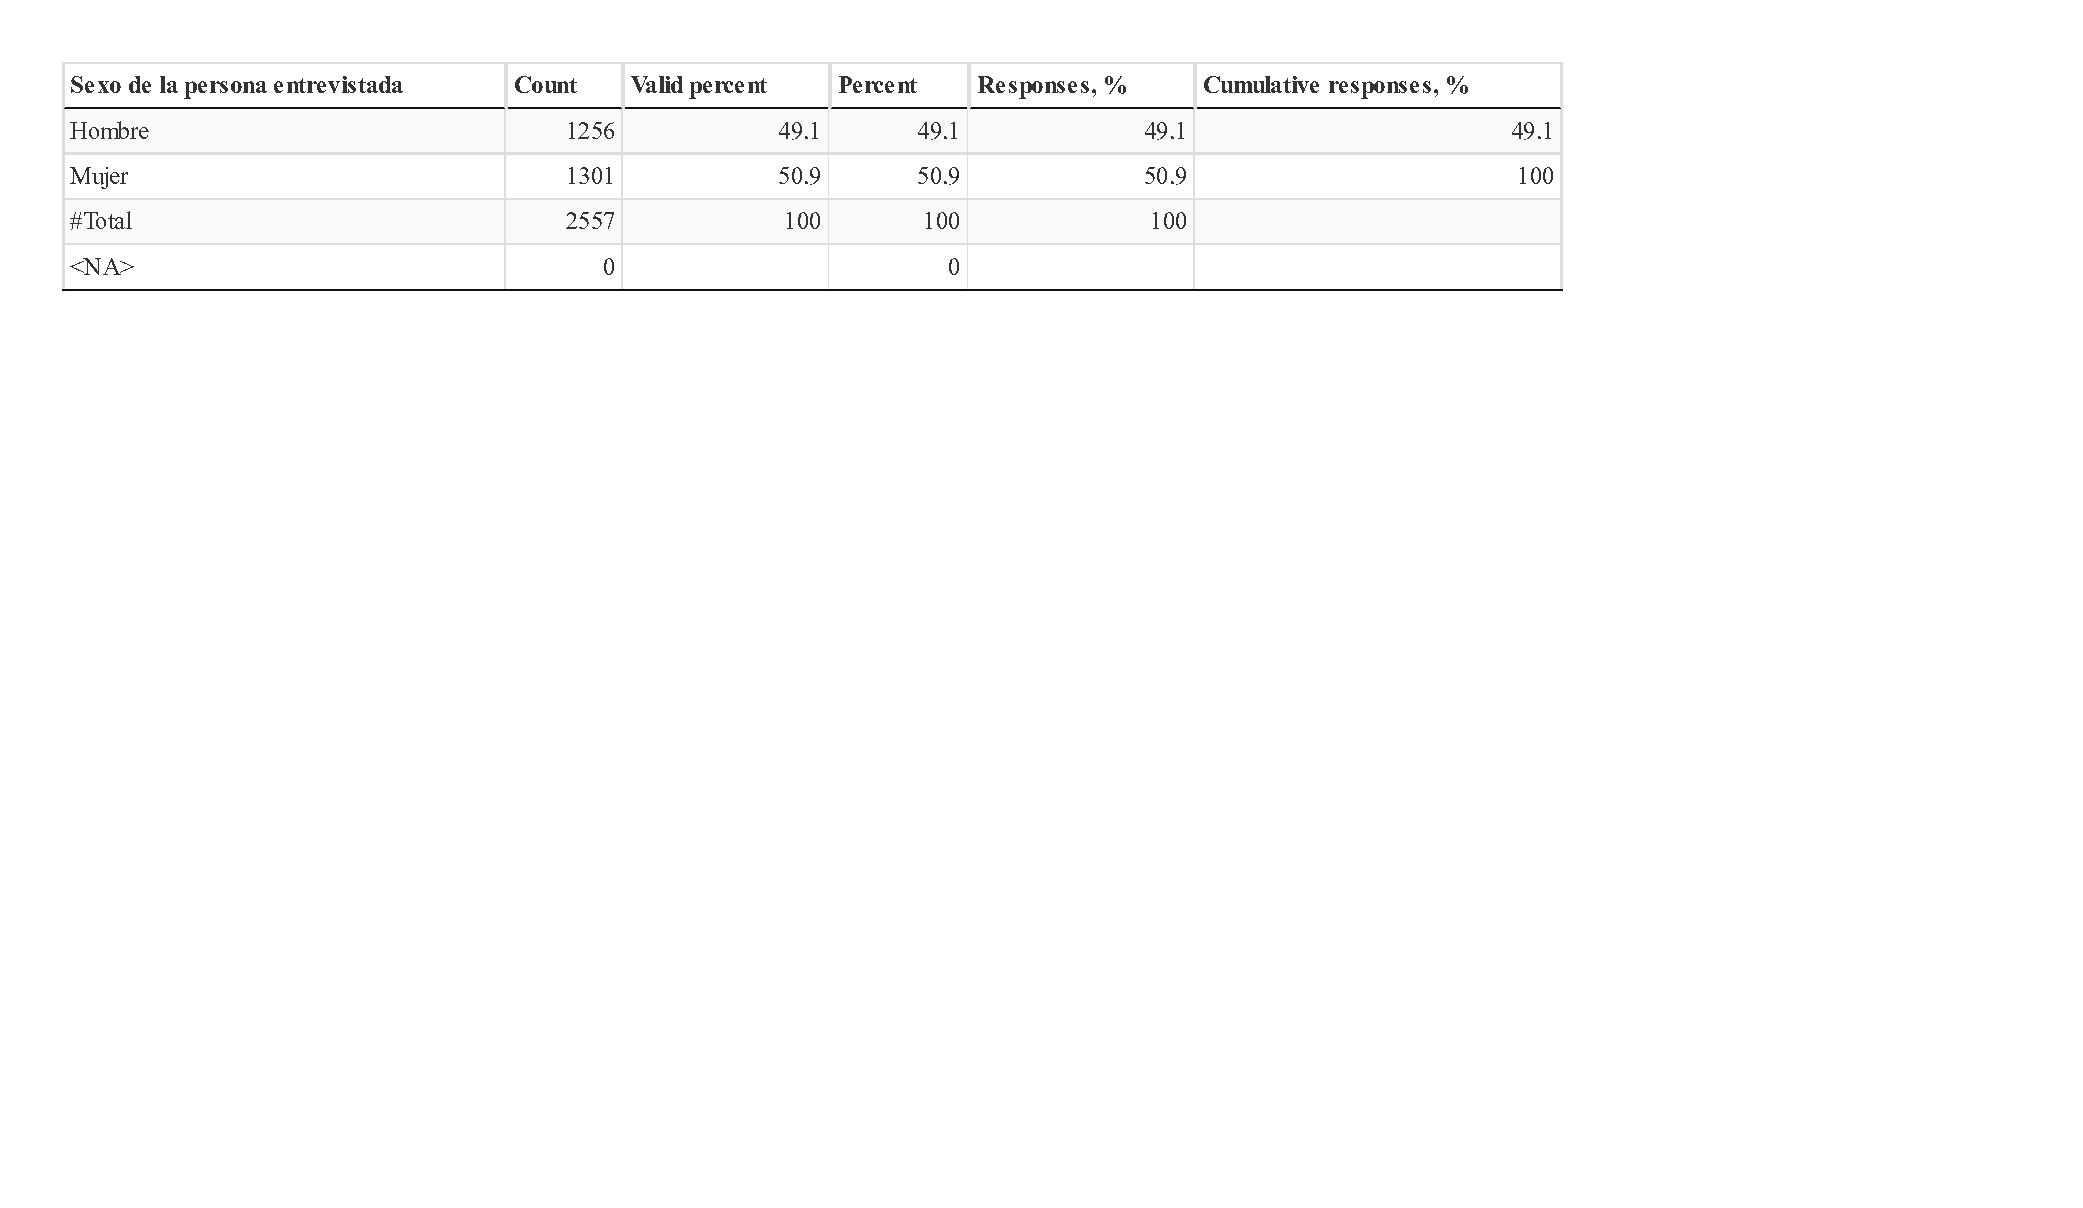
\includegraphics[width=0.95\linewidth]{Tablas-y-graficos-con-R-y-RStudio_files/figure-latex/unnamed-chunk-4-1} 

}

\caption{Frecuencias marginales de P31, estilo SPSS}\label{fig:unnamed-chunk-4}
\end{figure}

Alternativamente se puede presentar la forma que trabajaremos a lo largo de este curso, esta forma es la denominada script encadenado, donde definimos el marco de datos al inicio, y encadenamos instrucciones con el símbolo \%\textgreater\% que irían línea a línea sucesivamente para una mejor lectura y comprensión del texto escrito; podrían perfectamente ir en una línea. Nótese que la tabla sale igual con las dos formas, pero mientras que en el primer caso se usa la nomenclatura estándar de R, y el campo se llama \texttt{data\$P31}, es decir nombre del marco de datos en R (data) el símbolo del \texttt{\$} que separa y nombre del campo en el marco de datos \texttt{P31} en la segunda al definir de inicio que se utilizará \texttt{data} ya se usa el nombre \texttt{P31} directamente, aunque debamos dar la orden de cálculo con el comando \texttt{calculate()}.

\begin{Shaded}
\begin{Highlighting}[]
\FunctionTok{as.datatable\_widget}\NormalTok{(data }\SpecialCharTok{\%\textgreater{}\%}
  \FunctionTok{calculate}\NormalTok{(}\FunctionTok{fre}\NormalTok{(P31)))}
\end{Highlighting}
\end{Shaded}

\begin{figure}[H]

{\centering 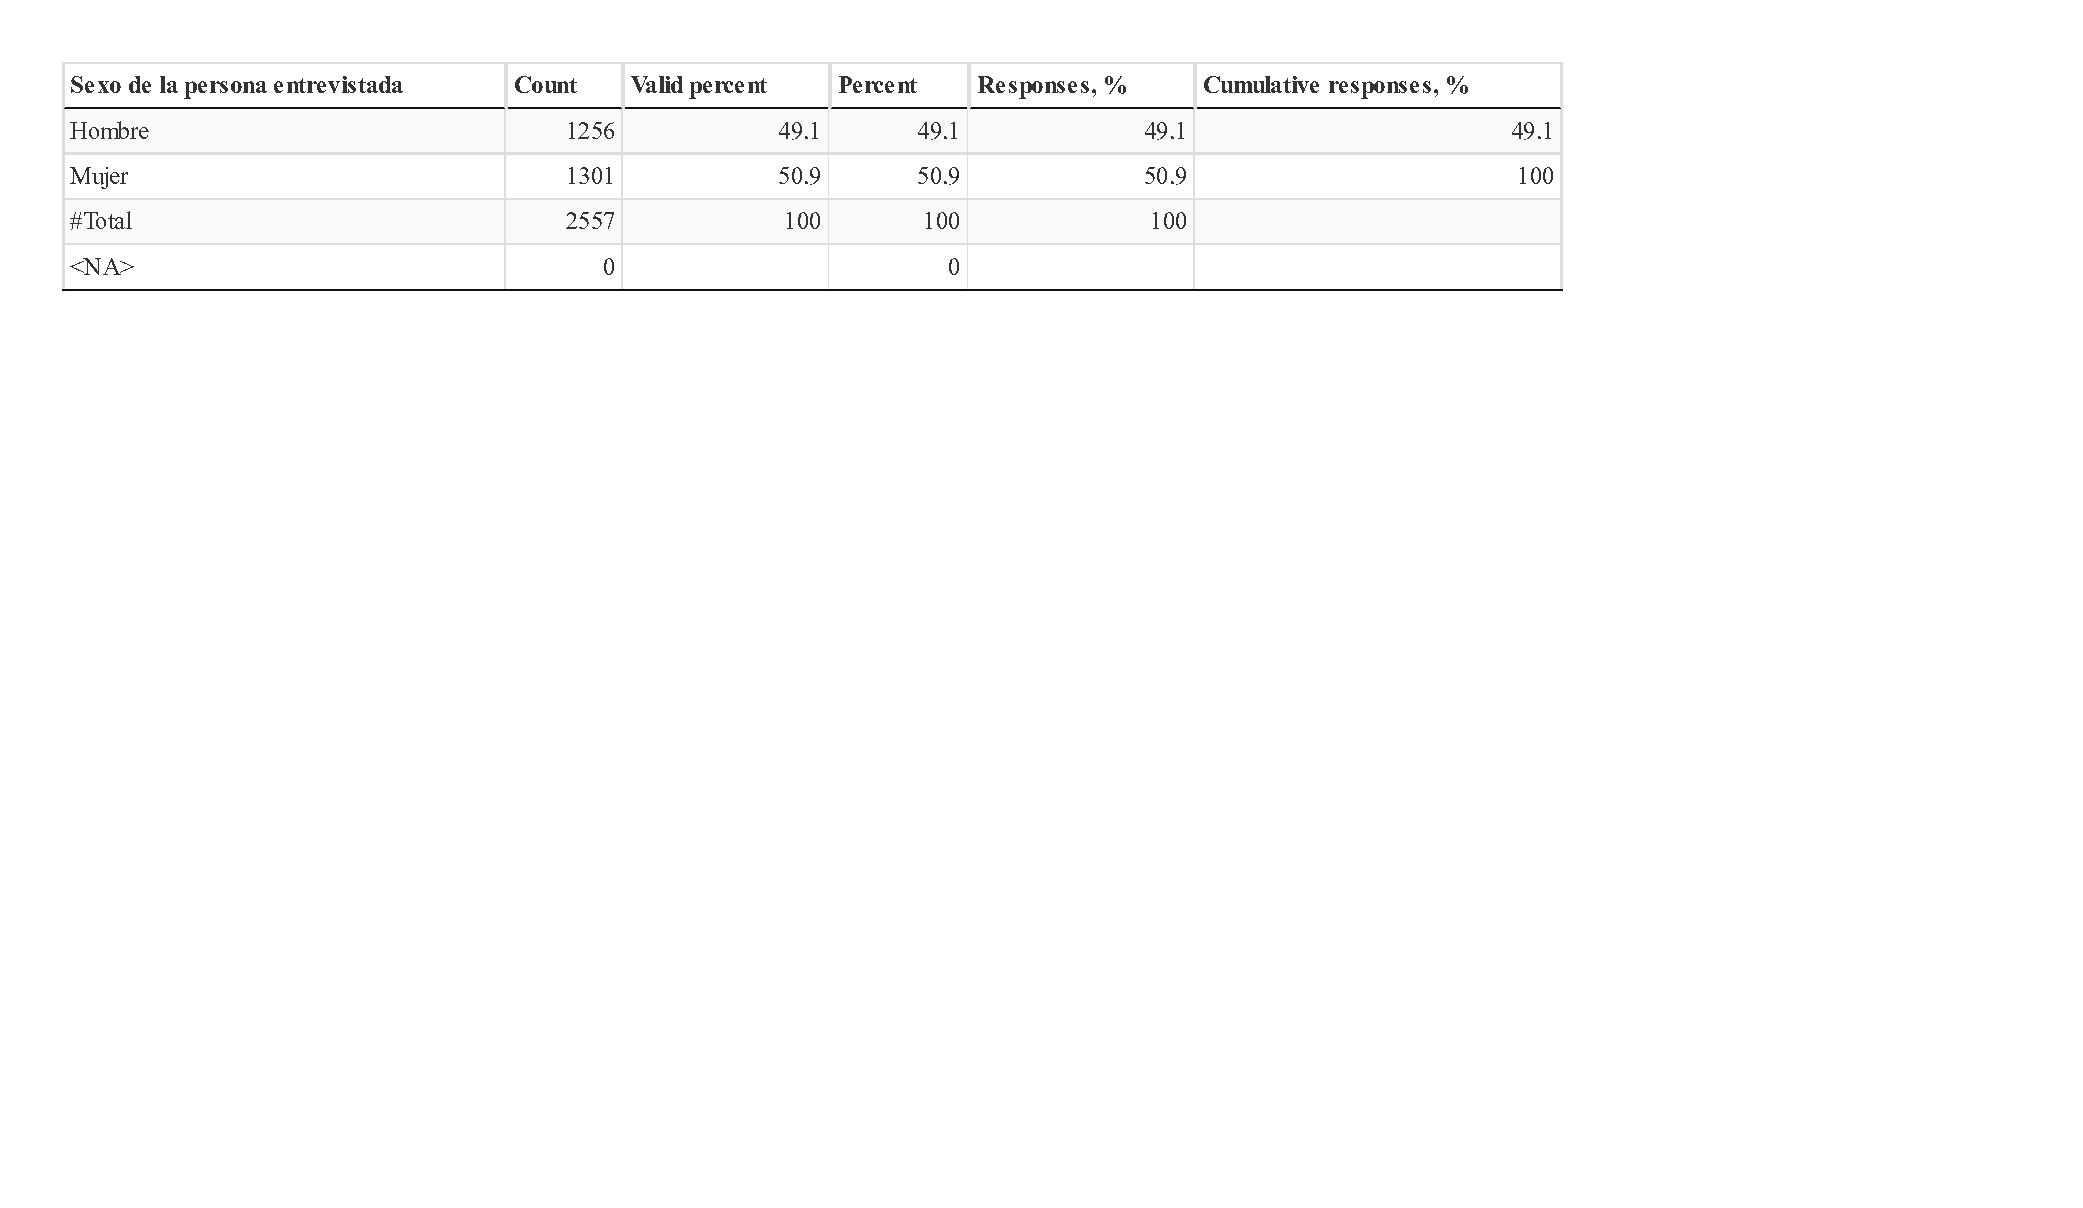
\includegraphics[width=0.95\linewidth]{Tablas-y-graficos-con-R-y-RStudio_files/figure-latex/unnamed-chunk-5-1} 

}

\caption{Frecuencias marginalesde P31 en tabla}\label{fig:unnamed-chunk-5}
\end{figure}

Veamos ahora cómo solicitaremos tablas de frecuencias, porcentajes y estadísticos simples con R.

\hypertarget{tablas-de-frecuencias-absolutos}{%
\subsubsection{Tablas de frecuencias (absolutos)}\label{tablas-de-frecuencias-absolutos}}

La segunda tabla que vamos a hacer, ya responde a la típica presentación de una tabla de contingencia, sólo que en este casos vamos a mostrar sólo un campo y por tanto no va a haber cruce de variables. En el paquete \texttt{expss}, para construir un cuadro deberemos indicar al menos:

\begin{itemize}
\tightlist
\item
  un marco de datos (\emph{dataframe} en nomenclatura R)
\item
  referenciar la variable sobre la que se deben calcular el estadístico seleccionado (frecuencia -casos-, media, mediana, máximo, mínimo\ldots)
\item
  una orden de impresión de tabla
\end{itemize}

Estos elementos básicos pueden completarse con campos de columnas, campos de filas, pruebas de significación, etc. Iremos desarrollando estos conceptos a lo largo de este documento. ¡Vamos a por el cuadro!

La que ahora entregamos, es la estructura básica de un script de R con el paquete \texttt{expss}. A lo largo del documento veremos cómo ir introduciendo mínimas variaciones a esta estructura que te permitirán descubrir un sinnúmero de posibilidades que ofrece este paquete de R. Por ejemplo, podemos modificar la etiqueta de TOTAL o indicar donde debe situarse la fila que contiene el cálculo TOTAL. Todas estas posibilidades las puedes conocer en la documentación original del \emph{package}, aunque en este manual trataremos de ir desgranado las más relevantes para nuestro objetivo. Inicialmente iremos añadiendo tras el operador \texttt{\%\textgreater{}\%} comentarios precedidos por el símbolo \texttt{\#}. Estos comentarios irán desapareciendo a medida que avancemos en el manual, y sólo se recurrirá a ellos cuando se aporte alguna nueva funcionalidad.

Para este primer script, indicaremos que usamos la fuente de datos (\emph{dataframe}) ya cargado en el análisis. En R Studio, el \emph{dataframe} tendrá el nombre que le hayas indicado en la carga -en nuestro caso \emph{data}-. Redactamos pues nuestro script, donde identificamos el \emph{dataframe}, el campo \texttt{P31} del cual vamos a calcular el número de casos:

\begin{Shaded}
\begin{Highlighting}[]
\FunctionTok{as.datatable\_widget}\NormalTok{(data }\SpecialCharTok{\%\textgreater{}\%}
  \FunctionTok{tab\_cells}\NormalTok{(P31) }\SpecialCharTok{\%\textgreater{}\%}
  \FunctionTok{tab\_stat\_cases}\NormalTok{() }\SpecialCharTok{\%\textgreater{}\%}
  \FunctionTok{tab\_pivot}\NormalTok{())}
\end{Highlighting}
\end{Shaded}

\begin{figure}[H]

{\centering 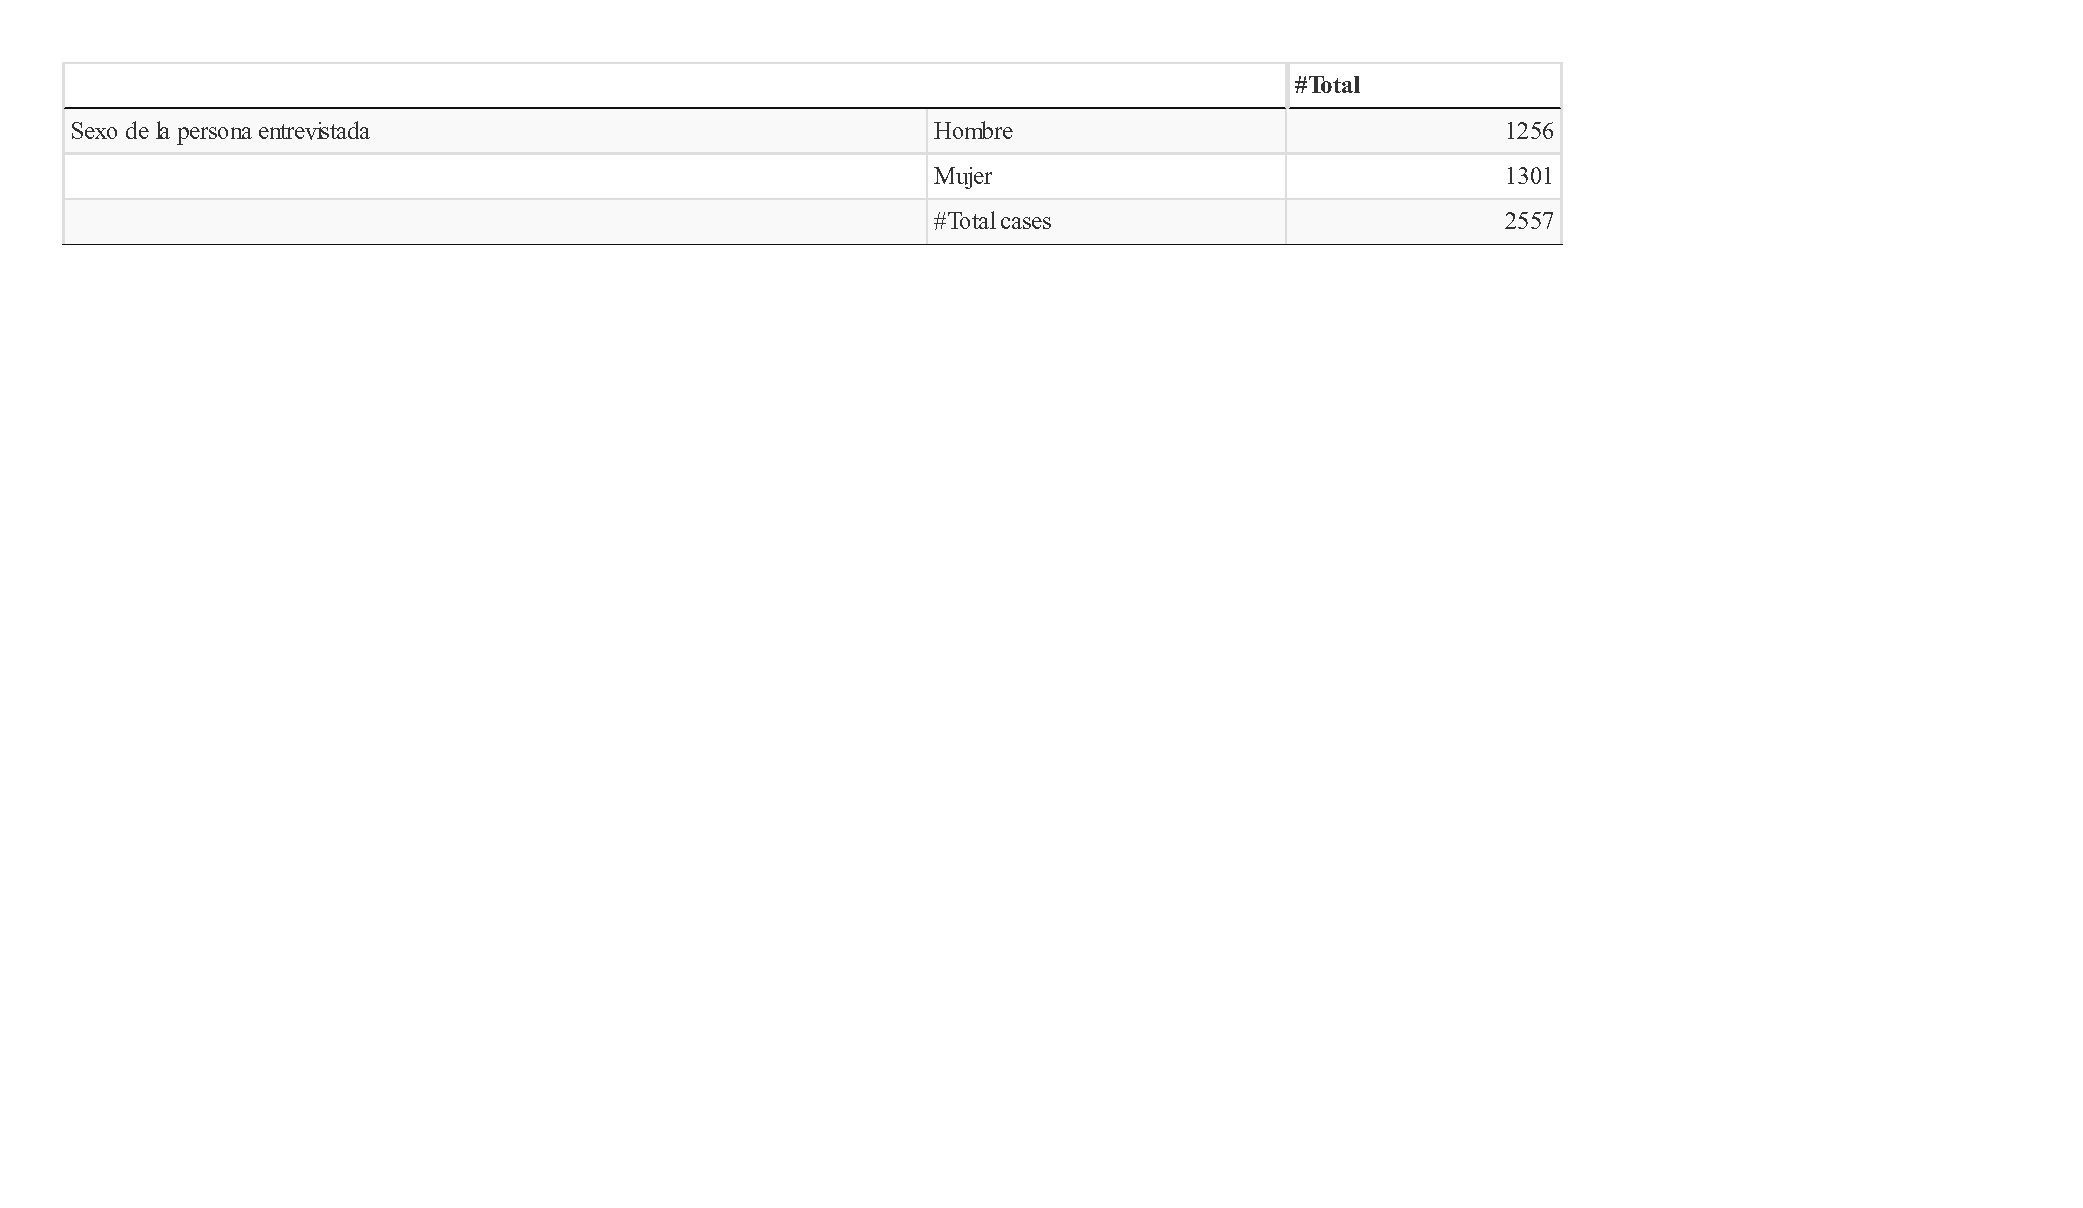
\includegraphics[width=0.95\linewidth]{Tablas-y-graficos-con-R-y-RStudio_files/figure-latex/unnamed-chunk-6-1} 

}

\caption{Frecuencias de P31}\label{fig:unnamed-chunk-6}
\end{figure}

Realicemos ahora una pequeña pero importante variación en el cálculo del estadístico casos -frecuencias- y utilicemos la posibilidad de ubicar donde queramos el total de casos, así como su etiqueta. Ello lo hacemos con \texttt{total\_row\_position\ =\ "above",\ label\ =\ "Casos"} aplicado a la función \texttt{tab\_stat\_cases()}.

\begin{Shaded}
\begin{Highlighting}[]
\FunctionTok{as.datatable\_widget}\NormalTok{(data }\SpecialCharTok{\%\textgreater{}\%}
  \FunctionTok{tab\_cells}\NormalTok{(P31) }\SpecialCharTok{\%\textgreater{}\%}
  \FunctionTok{tab\_stat\_cases}\NormalTok{(}\AttributeTok{total\_row\_position =} \StringTok{"above"}\NormalTok{, }\AttributeTok{label =} \StringTok{"Casos"}\NormalTok{) }\SpecialCharTok{\%\textgreater{}\%}
  \FunctionTok{tab\_pivot}\NormalTok{())}
\end{Highlighting}
\end{Shaded}

\begin{figure}[H]

{\centering 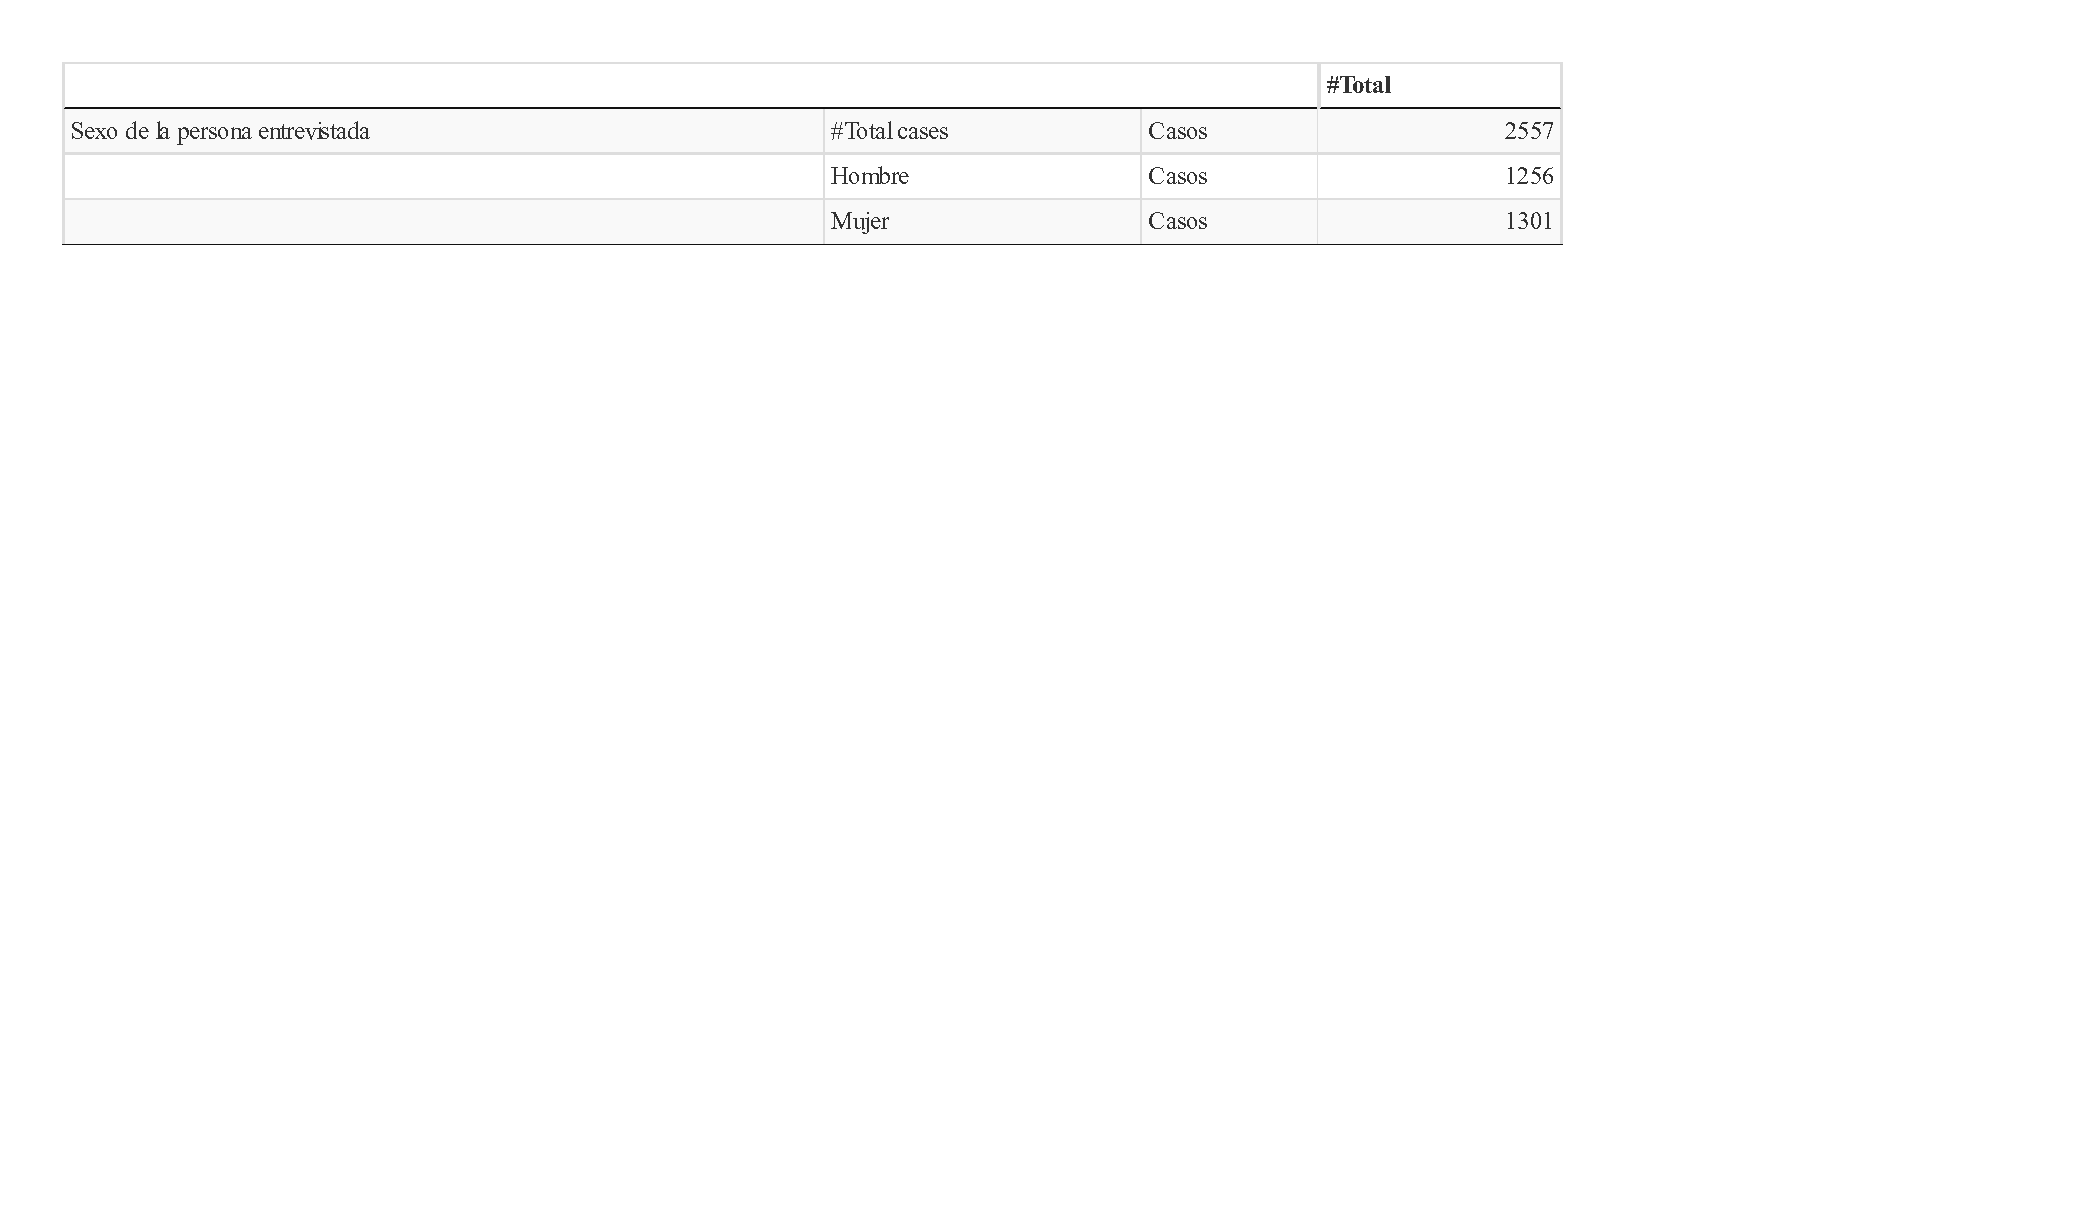
\includegraphics[width=0.95\linewidth]{Tablas-y-graficos-con-R-y-RStudio_files/figure-latex/unnamed-chunk-7-1} 

}

\caption{Frecuencias de P31, moviendo el Total}\label{fig:unnamed-chunk-7}
\end{figure}

\hypertarget{tablas-de-frecuencias-relativas}{%
\subsubsection{Tablas de frecuencias relativas}\label{tablas-de-frecuencias-relativas}}

Si en lugar de obtener casos (valores absolutos) queremos sacar valores porcentuales, el cambio es mínimo. Usaremos el comando \texttt{tab\_stat\_cpct()}para indicarlo.

\begin{Shaded}
\begin{Highlighting}[]
\FunctionTok{as.datatable\_widget}\NormalTok{(data }\SpecialCharTok{\%\textgreater{}\%}
  \FunctionTok{tab\_cells}\NormalTok{(P31) }\SpecialCharTok{\%\textgreater{}\%}
  \FunctionTok{tab\_stat\_cpct}\NormalTok{(}\AttributeTok{total\_row\_position =} \StringTok{"above"}\NormalTok{, }\AttributeTok{label =} \StringTok{"\% casos"}\NormalTok{) }\SpecialCharTok{\%\textgreater{}\%}
  \FunctionTok{tab\_pivot}\NormalTok{())}
\end{Highlighting}
\end{Shaded}

\begin{figure}[H]

{\centering 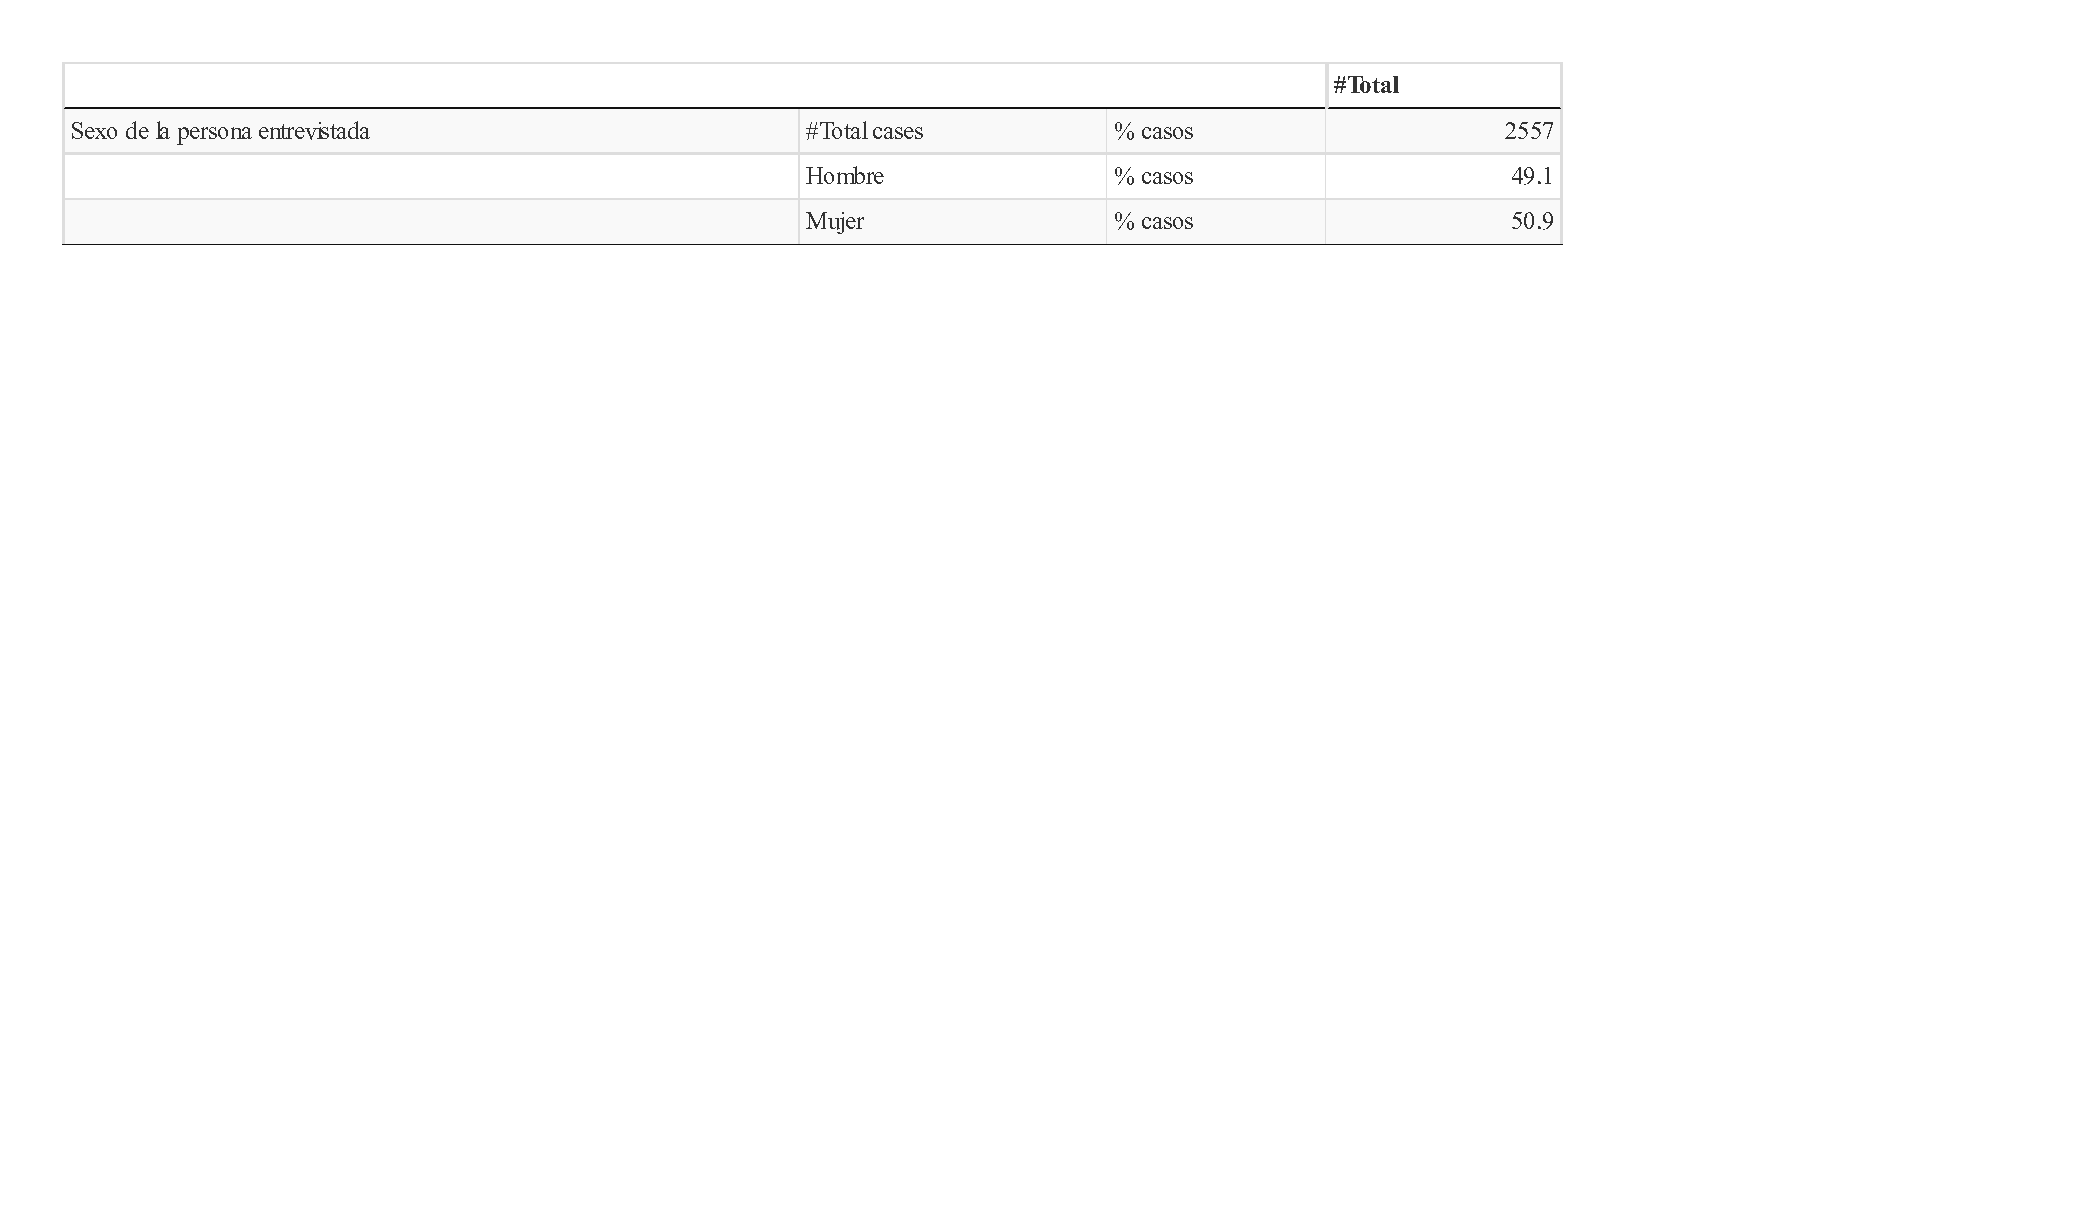
\includegraphics[width=0.95\linewidth]{Tablas-y-graficos-con-R-y-RStudio_files/figure-latex/unnamed-chunk-8-1} 

}

\caption{Porcentajes de P31}\label{fig:unnamed-chunk-8}
\end{figure}

\hypertarget{tablas-de-absolutos-y-realativos-juntos}{%
\subsubsection{Tablas de absolutos y realativos (juntos)}\label{tablas-de-absolutos-y-realativos-juntos}}

Cuando deseamos hacer combinaciones de frecuencias y porcentajes, la filosofía de trabajo es muy parecida. En nuestro caso vamos a hacer algo muy típico. Aunque creo que resulta más sencillo leer cada estadístico en su tabla, hay ocasiones en las que la comparativa es muy necesaria y por tanto es necesario unir los estadísticos en la misma tabla. Nótese la diferencia con el siguiente cuadro\ldots{}

\begin{Shaded}
\begin{Highlighting}[]
\FunctionTok{as.datatable\_widget}\NormalTok{(data }\SpecialCharTok{\%\textgreater{}\%}
  \FunctionTok{tab\_cells}\NormalTok{(P31) }\SpecialCharTok{\%\textgreater{}\%}
  \FunctionTok{tab\_stat\_cases}\NormalTok{(}\AttributeTok{total\_row\_position =} \StringTok{"above"}\NormalTok{, }\AttributeTok{label =} \StringTok{"Casos"}\NormalTok{) }\SpecialCharTok{\%\textgreater{}\%}
  \FunctionTok{tab\_stat\_cpct}\NormalTok{(}\AttributeTok{label =} \StringTok{"\% casos"}\NormalTok{) }\SpecialCharTok{\%\textgreater{}\%}
  \FunctionTok{tab\_pivot}\NormalTok{(}\AttributeTok{stat\_position =} \StringTok{"inside\_columns"}\NormalTok{))}
\end{Highlighting}
\end{Shaded}

\begin{figure}[H]

{\centering 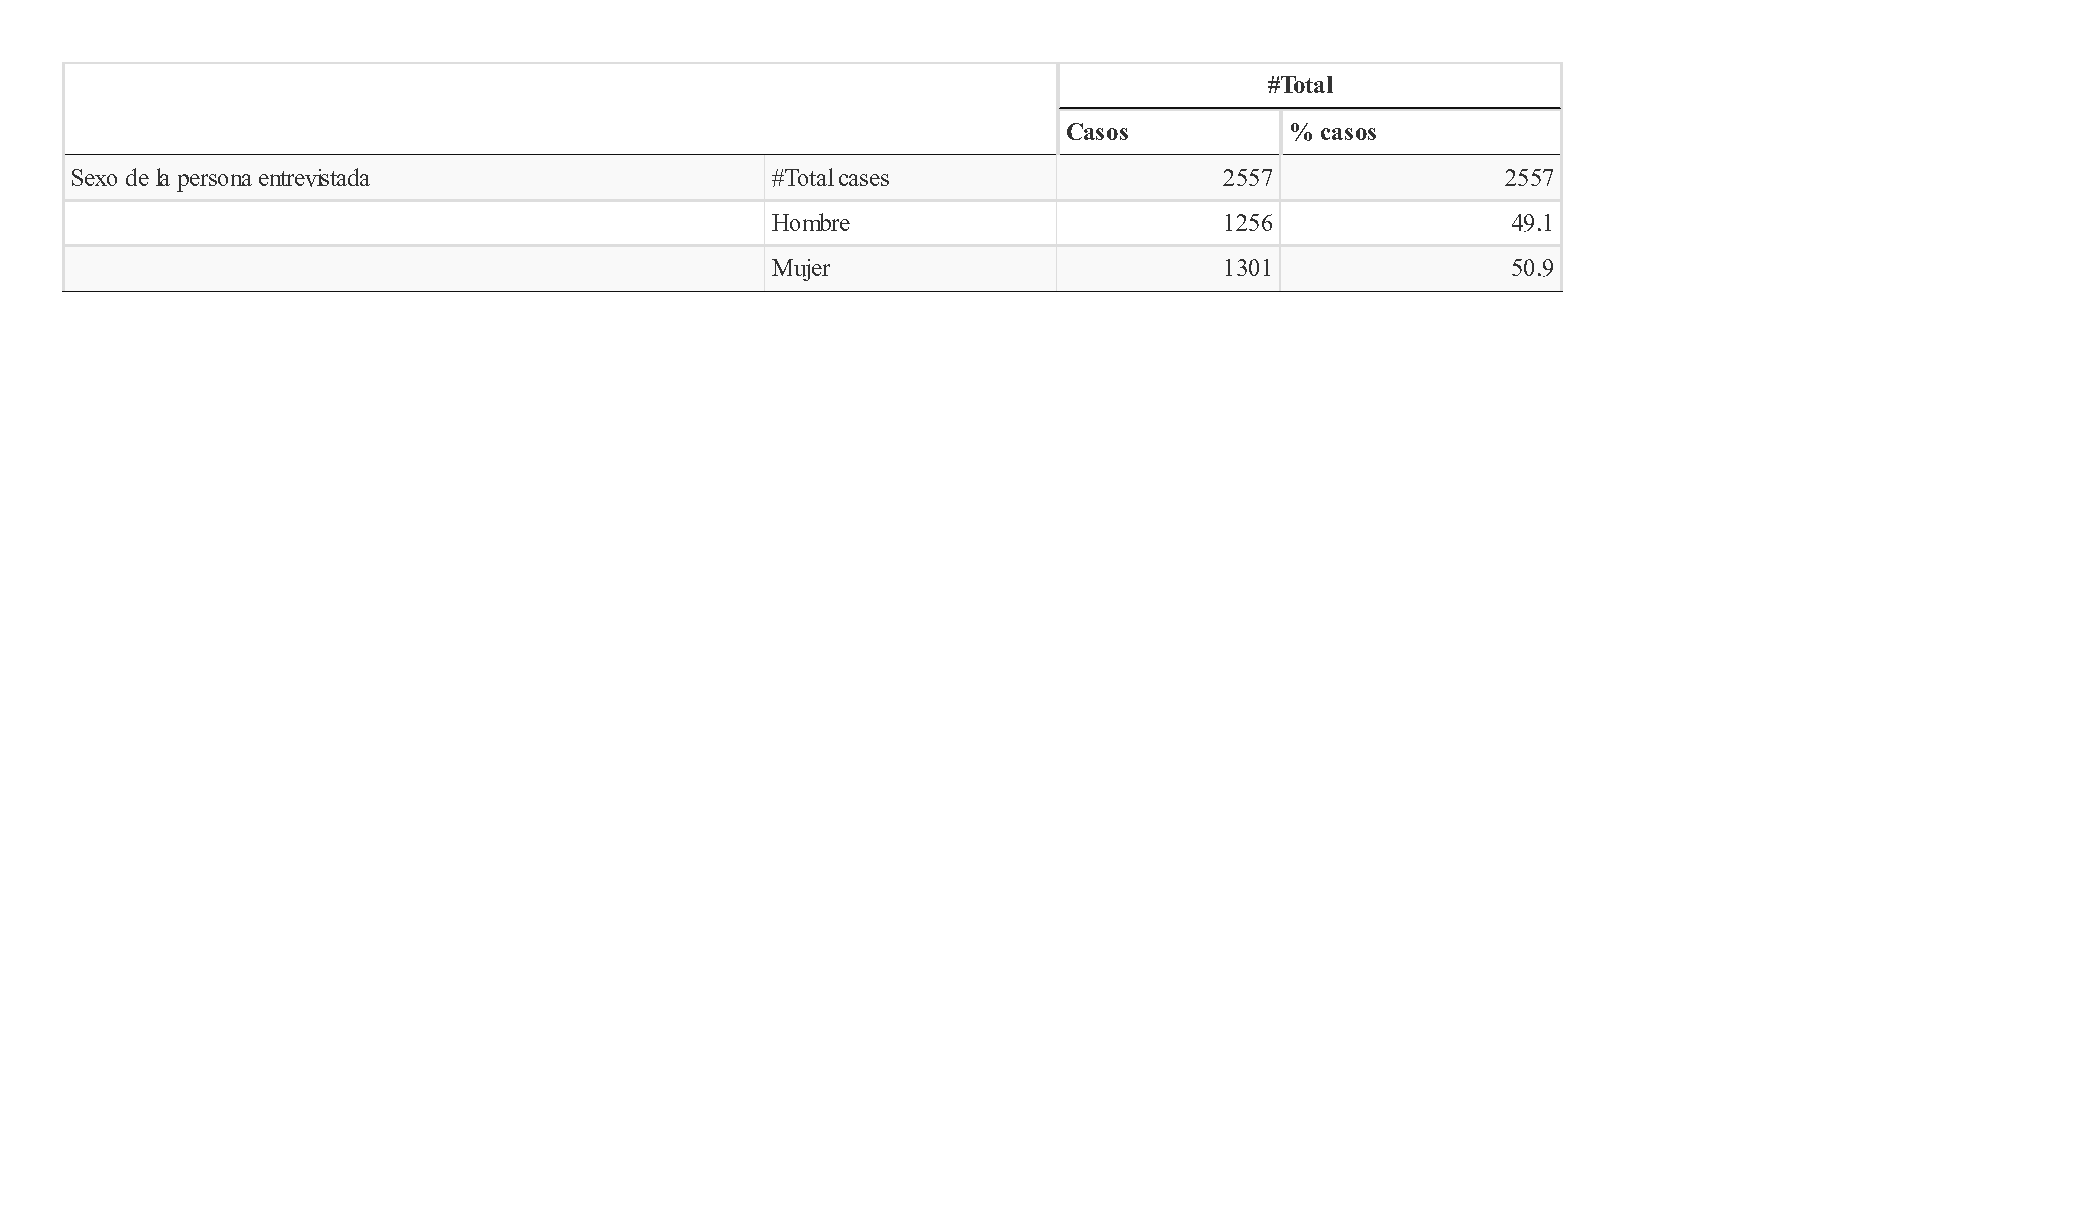
\includegraphics[width=0.95\linewidth]{Tablas-y-graficos-con-R-y-RStudio_files/figure-latex/unnamed-chunk-9-1} 

}

\caption{Frecuencias y porcentajes de P31}\label{fig:unnamed-chunk-9}
\end{figure}

Nótese el efecto introducido por el modificador de posición del cálculo. También \ldots{}

\begin{Shaded}
\begin{Highlighting}[]
\FunctionTok{as.datatable\_widget}\NormalTok{(data }\SpecialCharTok{\%\textgreater{}\%}
  \FunctionTok{tab\_cells}\NormalTok{(P31) }\SpecialCharTok{\%\textgreater{}\%}
  \FunctionTok{tab\_stat\_cases}\NormalTok{(}\AttributeTok{total\_row\_position =} \StringTok{"above"}\NormalTok{, }\AttributeTok{label =} \StringTok{"Casos"}\NormalTok{) }\SpecialCharTok{\%\textgreater{}\%}
  \FunctionTok{tab\_stat\_cpct}\NormalTok{(}\AttributeTok{label =} \StringTok{"\% casos"}\NormalTok{) }\SpecialCharTok{\%\textgreater{}\%}
  \FunctionTok{tab\_pivot}\NormalTok{(}\AttributeTok{stat\_position =} \StringTok{"outside\_rows"}\NormalTok{))}
\end{Highlighting}
\end{Shaded}

\begin{figure}[H]

{\centering 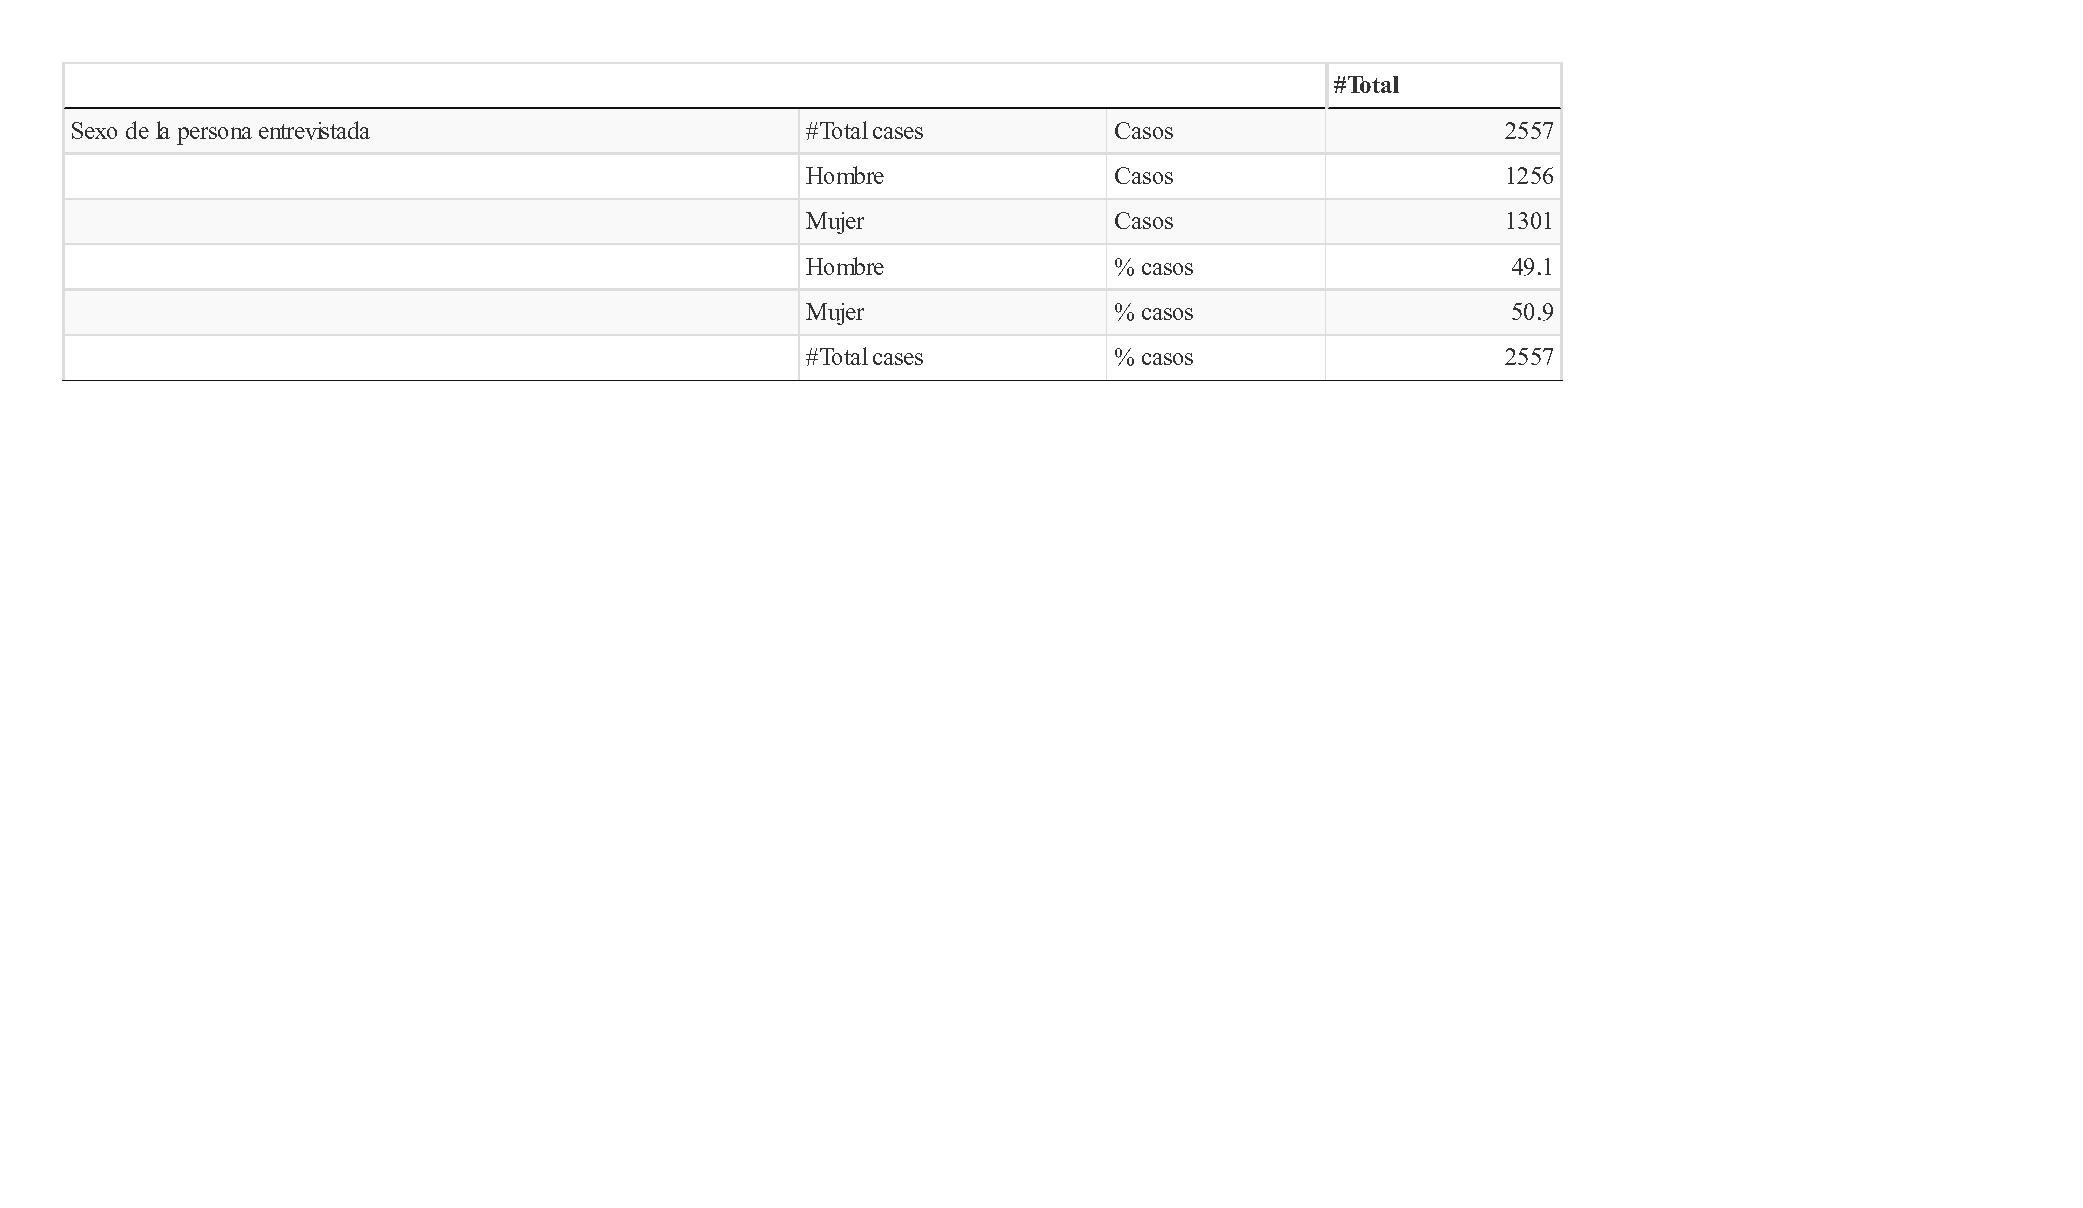
\includegraphics[width=0.95\linewidth]{Tablas-y-graficos-con-R-y-RStudio_files/figure-latex/unnamed-chunk-10-1} 

}

\caption{Tablas con propiedades diferentes a estándar}\label{fig:unnamed-chunk-10}
\end{figure}

O también \ldots{}

\begin{Shaded}
\begin{Highlighting}[]
\FunctionTok{as.datatable\_widget}\NormalTok{(data }\SpecialCharTok{\%\textgreater{}\%}
  \FunctionTok{tab\_cells}\NormalTok{(P31) }\SpecialCharTok{\%\textgreater{}\%}
  \FunctionTok{tab\_stat\_cases}\NormalTok{(}\AttributeTok{total\_row\_position =} \StringTok{"below"}\NormalTok{, }\AttributeTok{label =} \StringTok{"Casos"}\NormalTok{) }\SpecialCharTok{\%\textgreater{}\%}
  \FunctionTok{tab\_stat\_cpct}\NormalTok{(}\AttributeTok{label =} \StringTok{"\% casos"}\NormalTok{) }\SpecialCharTok{\%\textgreater{}\%}
  \FunctionTok{tab\_pivot}\NormalTok{(}\AttributeTok{stat\_position =} \StringTok{"inside\_columns"}\NormalTok{))}
\end{Highlighting}
\end{Shaded}

\begin{figure}[H]

{\centering 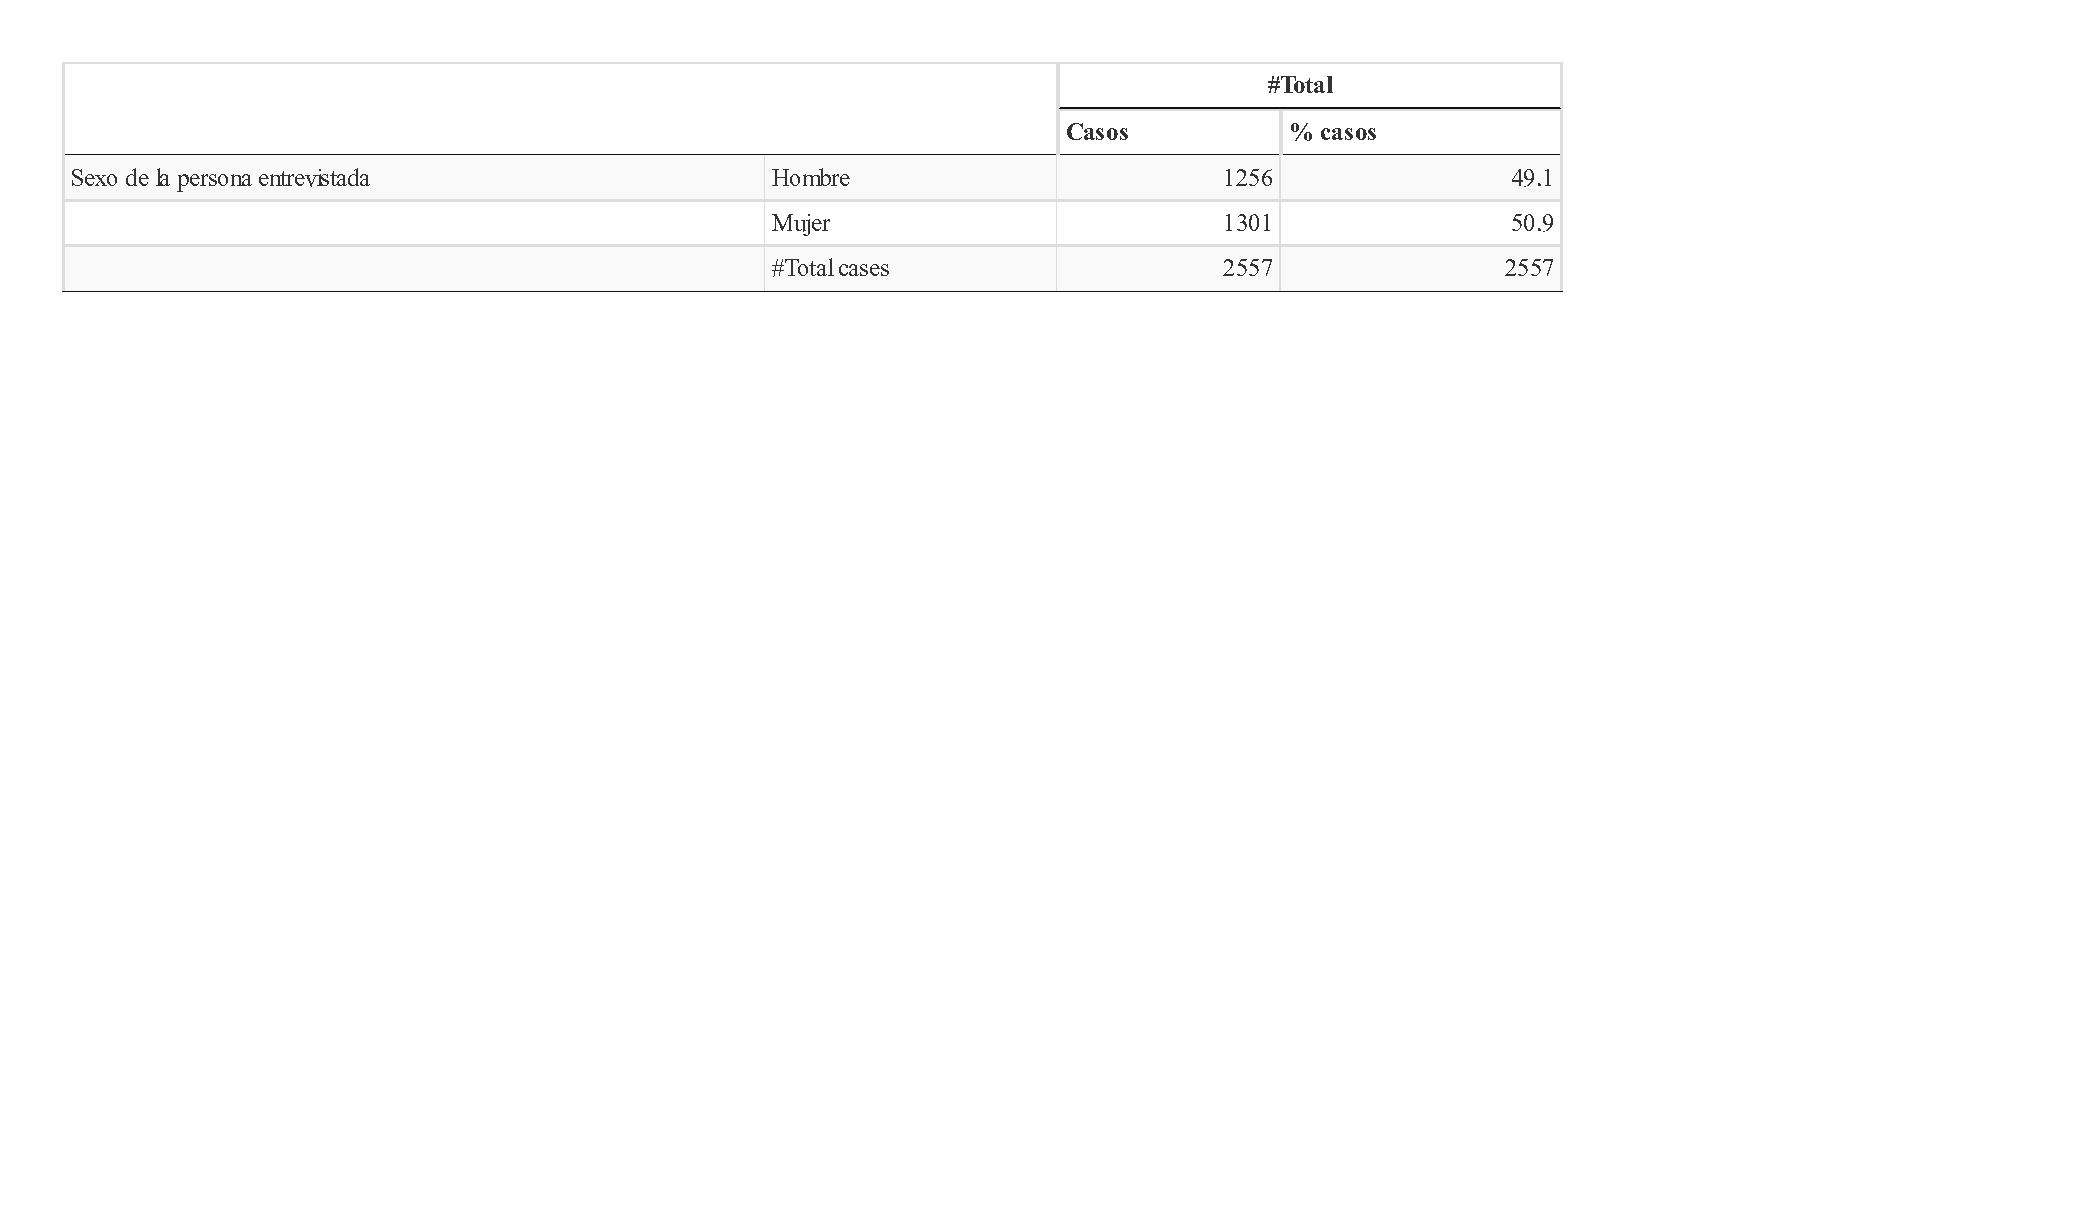
\includegraphics[width=0.95\linewidth]{Tablas-y-graficos-con-R-y-RStudio_files/figure-latex/unnamed-chunk-11-1} 

}

\caption{Propiedades diferentes al estándar}\label{fig:unnamed-chunk-11}
\end{figure}

\hypertarget{variable-de-respuesta-muxfaltiple}{%
\subsection{Variable de respuesta múltiple}\label{variable-de-respuesta-muxfaltiple}}

Vamos a trabajar ahora con variables multi respuesta. Para trabajar con múltiples, debemos conocer en qué forma nos llegan en nuestro \emph{input}. Por ejemplo, \texttt{SPSS} divide la variable múltiple en tantas variables simples (o dicotómicas binarias) como requiera para poder representar la multi respuesta. Por ejemplo, si tenemos una variable múltiple denominada P01, y el máximo número de respuestas (menciones) en el banco de datos es 3, al crear el \texttt{\_dataframe\_} se crean las variables P01\_1, P01\_2 y P01\_3; es con estas variables con las que trabajamos. Cada una de estas variables puede tomar cualquiera de los valores codificados.

Para \texttt{expss}, la forma de indicar que un conjunto de campos forman una multi respuesta es muy simple anteponer \texttt{mrset\_f()} al nombre del campo que vamos a usar. Debemos tener la precaución de que no haya variables en el banco de datos que comiencen por la misma raíz. Así, el campo de ejemplo sería \texttt{mrset\_f(P01\_)} y con eso procesaría las tres variables de forma conjunta. Alternativamente, podríamos usar también:

\begin{itemize}
\tightlist
\item
  mrset(P01\_1 \%to\% P01\_3) o también,
\item
  mrset(P01\_1,P01\_2,P01\_3)
\end{itemize}

Cualquiera de ellas sería también válida, pero nótese que en estas últimas listadas, es necesario saber donde empieza y acaba la múltiple y esto puede variar sobretodo si creamos los script antes de acabar el campo. Al acabar el campo, pudiera haber algún nuevo caso que tuviera más menciones que 3 y por tanto existirían también \_4, \_5 o, \_n.

Como hemos indicado, no olvides que existe otra forma de trabajar las múltiples, utilizando variables dicotómicas o binarias (así es como están en nuestro banco de datos del CIS). En este caso, serviría todo lo afirmado anteriormente, pero en lugar de \texttt{mrset\_f()}, usaríamos \texttt{mdset\_f()}.

\hypertarget{tablas-de-frecuencias-absolutas}{%
\subsubsection{Tablas de frecuencias absolutas}\label{tablas-de-frecuencias-absolutas}}

Usaremos el campo P18C para procesar su información, que se localiza en el banco de datos desde P18C01 hasta P18C08.

\begin{Shaded}
\begin{Highlighting}[]
\FunctionTok{as.datatable\_widget}\NormalTok{(data }\SpecialCharTok{\%\textgreater{}\%}
  \FunctionTok{tab\_cells}\NormalTok{(}\FunctionTok{mdset\_f}\NormalTok{(P18C)) }\SpecialCharTok{\%\textgreater{}\%}
  \FunctionTok{tab\_stat\_cases}\NormalTok{(}\AttributeTok{total\_row\_position =} \StringTok{"above"}\NormalTok{, }\AttributeTok{label =} \StringTok{"Casos"}\NormalTok{) }\SpecialCharTok{\%\textgreater{}\%}
  \FunctionTok{tab\_pivot}\NormalTok{(}\AttributeTok{stat\_position =} \StringTok{"inside\_columns"}\NormalTok{))}
\end{Highlighting}
\end{Shaded}

\begin{figure}[H]

{\centering 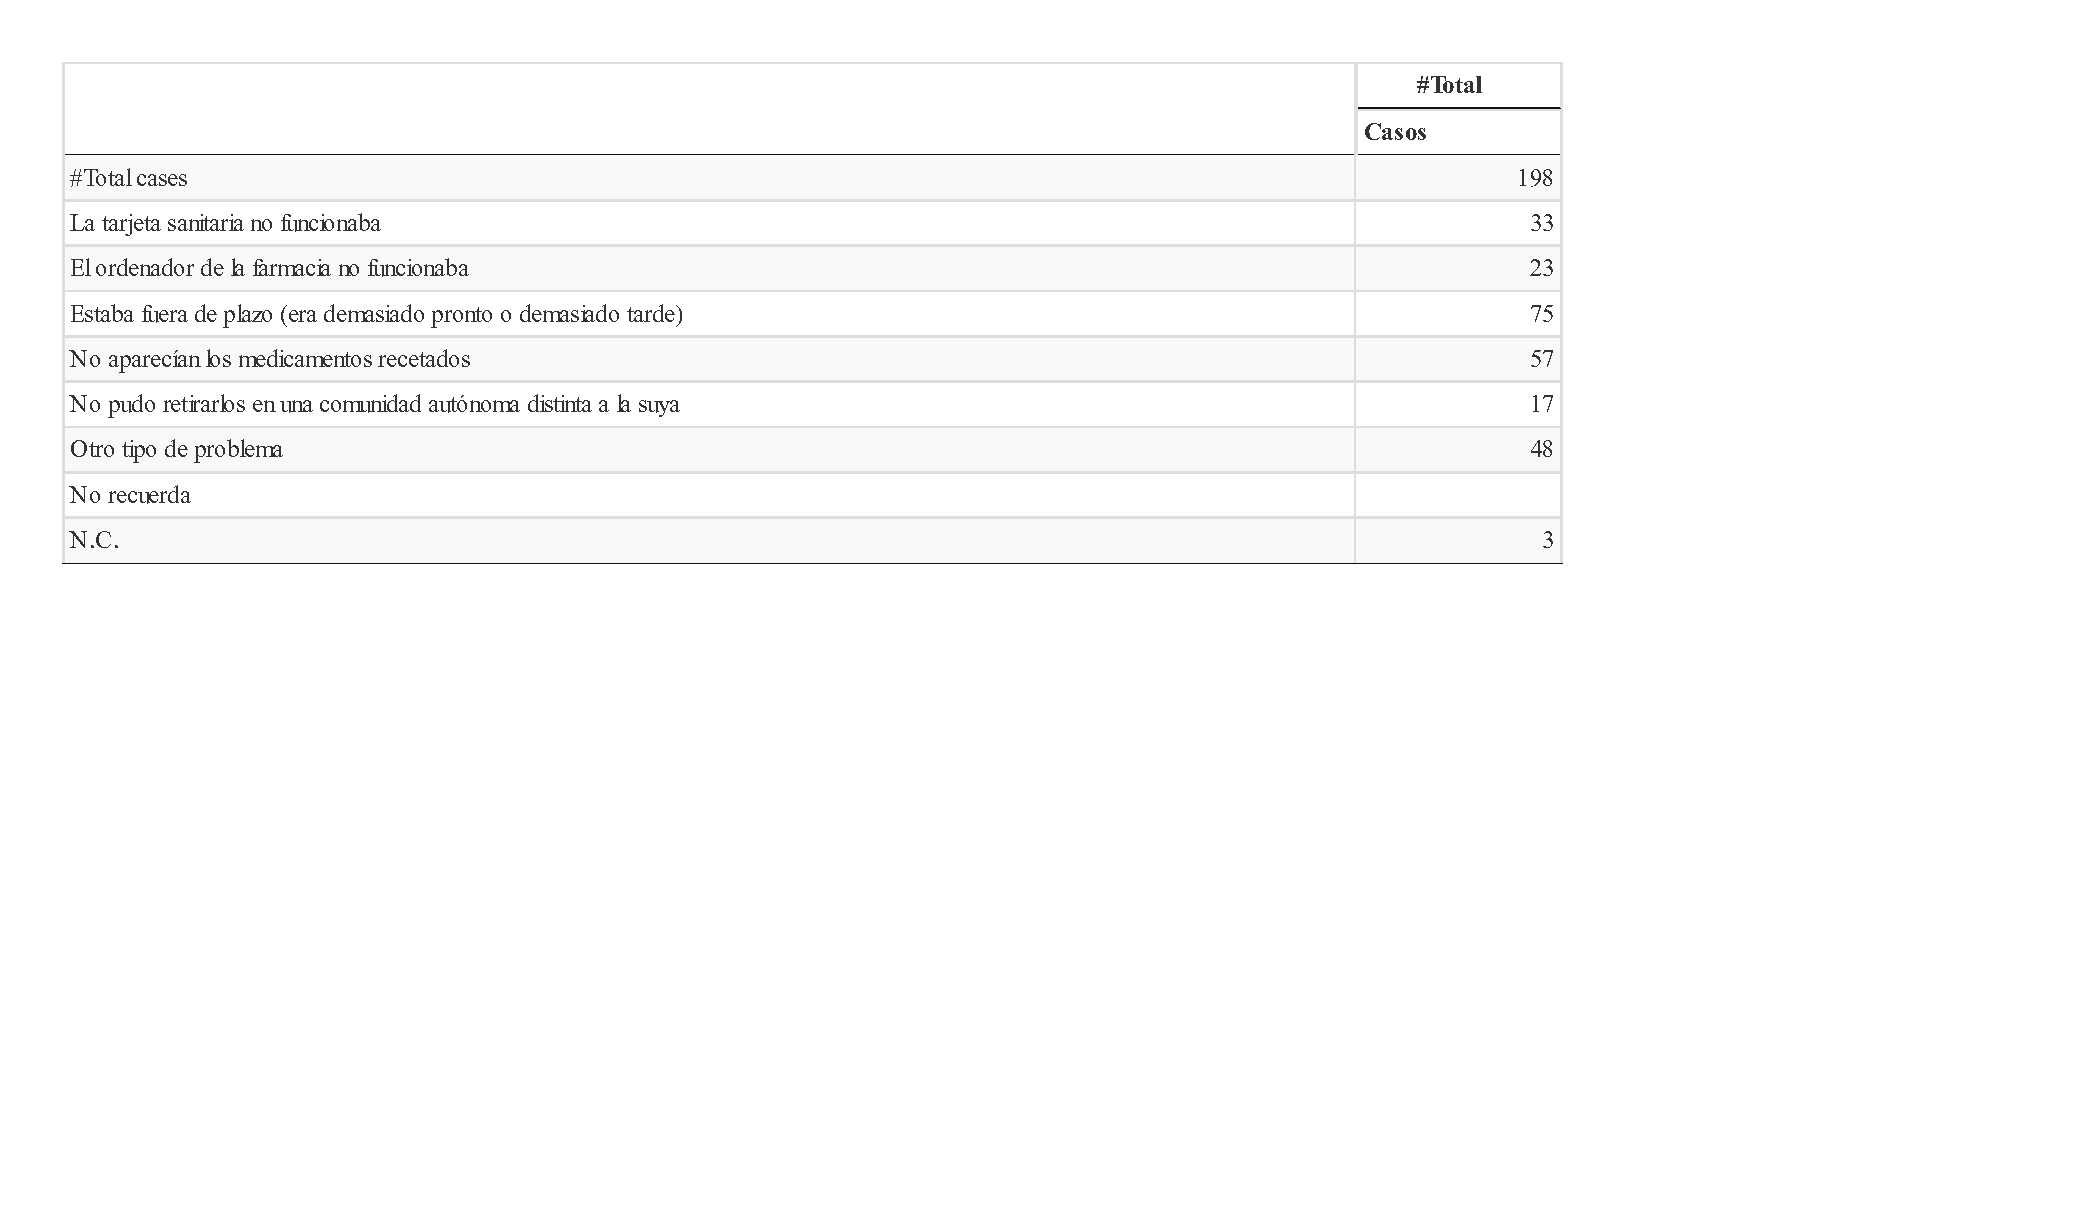
\includegraphics[width=0.95\linewidth]{Tablas-y-graficos-con-R-y-RStudio_files/figure-latex/unnamed-chunk-12-1} 

}

\caption{Frecuencias de P18}\label{fig:unnamed-chunk-12}
\end{figure}

\hypertarget{tablas-de-frecuencias-relativas-1}{%
\subsubsection{Tablas de frecuencias relativas}\label{tablas-de-frecuencias-relativas-1}}

También se pueden, como es obvio, obtener porcentajes en las tablas marginales múltiples. A diferencia de cuando la variables es simple que todos los porcentajes suman 100, en las variables múltiples cada alternativa tiene un rango de 0 a 100, desde no ser elegida una opción en ningún registro del \texttt{\_dataframe\_}, hasta ser elegida por todos los registros. Usaremos nuevamente el campo P18C para procesar su información, que se localiza en el banco de datos desde P18C01 hasta P18C08.

\begin{Shaded}
\begin{Highlighting}[]
\FunctionTok{as.datatable\_widget}\NormalTok{(data }\SpecialCharTok{\%\textgreater{}\%}
  \FunctionTok{tab\_cells}\NormalTok{(}\FunctionTok{mdset\_f}\NormalTok{(P18C)) }\SpecialCharTok{\%\textgreater{}\%}
  \FunctionTok{tab\_stat\_cpct}\NormalTok{(}\AttributeTok{total\_row\_position =} \StringTok{"above"}\NormalTok{, }\AttributeTok{label =} \StringTok{"\% casos"}\NormalTok{) }\SpecialCharTok{\%\textgreater{}\%}
  \FunctionTok{tab\_pivot}\NormalTok{(}\AttributeTok{stat\_position =} \StringTok{"inside\_columns"}\NormalTok{))}
\end{Highlighting}
\end{Shaded}

\begin{figure}[H]

{\centering 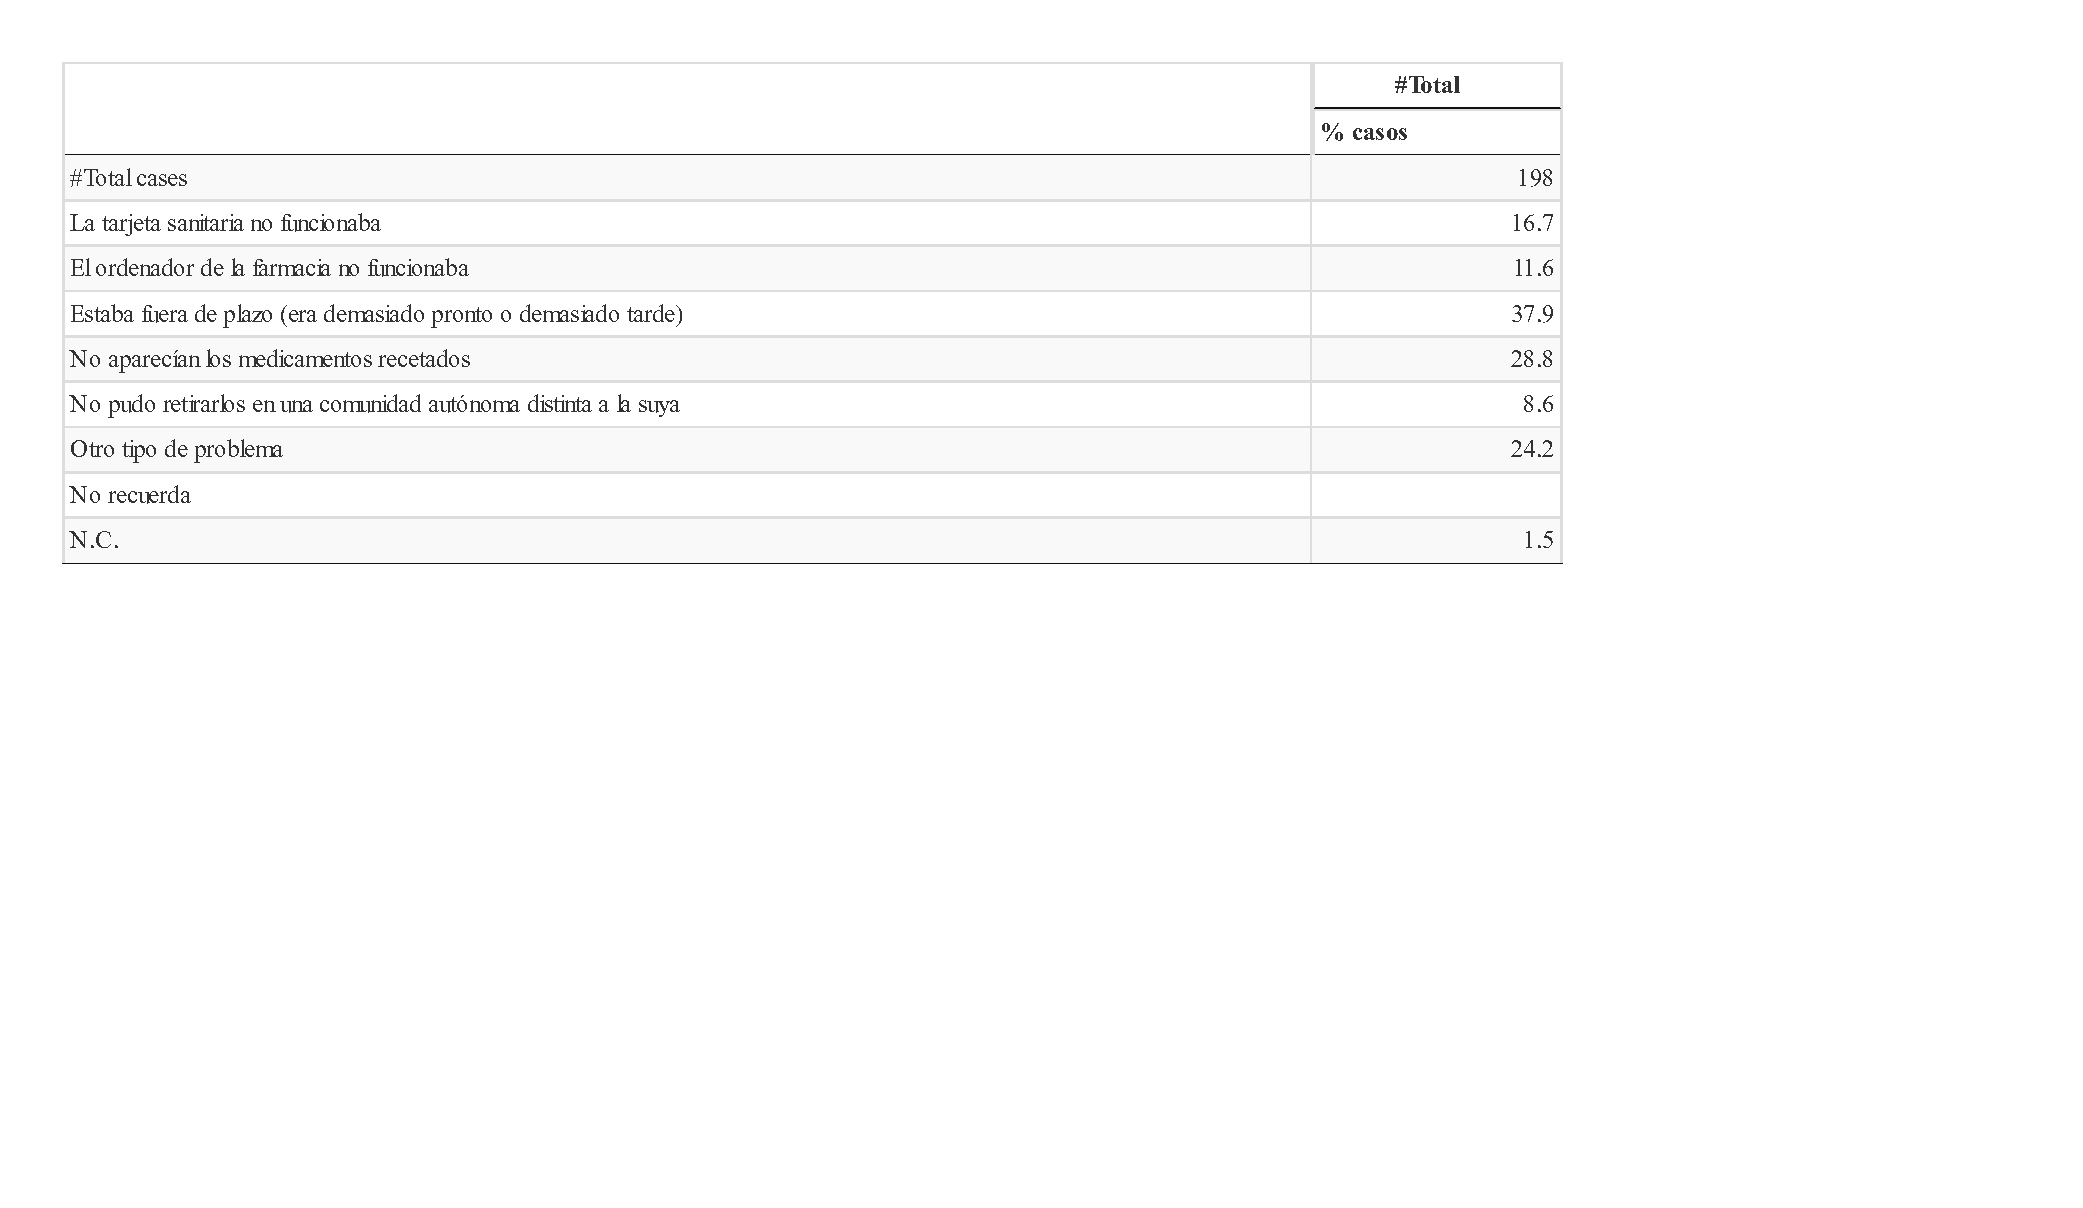
\includegraphics[width=0.95\linewidth]{Tablas-y-graficos-con-R-y-RStudio_files/figure-latex/unnamed-chunk-13-1} 

}

\caption{Frecuencias de P18}\label{fig:unnamed-chunk-13}
\end{figure}

Pero vamos a introducir una nueva variación. En una múltiple, también pueden calcularse los resultados en lo que se llama \texttt{base\ respuestas}, donde sí suman 100\% los porcentajes nuevamente, pero recuerda que el porcentaje hace referencia a las respuestas, no a los individuos. En este caso el script modifica el estadístico solicitado.

\begin{Shaded}
\begin{Highlighting}[]
\FunctionTok{as.datatable\_widget}\NormalTok{(data }\SpecialCharTok{\%\textgreater{}\%}
  \FunctionTok{tab\_cells}\NormalTok{(}\FunctionTok{mdset\_f}\NormalTok{(P18C)) }\SpecialCharTok{\%\textgreater{}\%}
  \FunctionTok{tab\_stat\_cpct\_responses}\NormalTok{(}\AttributeTok{total\_row\_position =} \StringTok{"above"}\NormalTok{,}
    \AttributeTok{label =} \StringTok{"\% casos"}\NormalTok{) }\SpecialCharTok{\%\textgreater{}\%}
  \FunctionTok{tab\_pivot}\NormalTok{(}\AttributeTok{stat\_position =} \StringTok{"inside\_columns"}\NormalTok{))}
\end{Highlighting}
\end{Shaded}

\begin{figure}[H]

{\centering 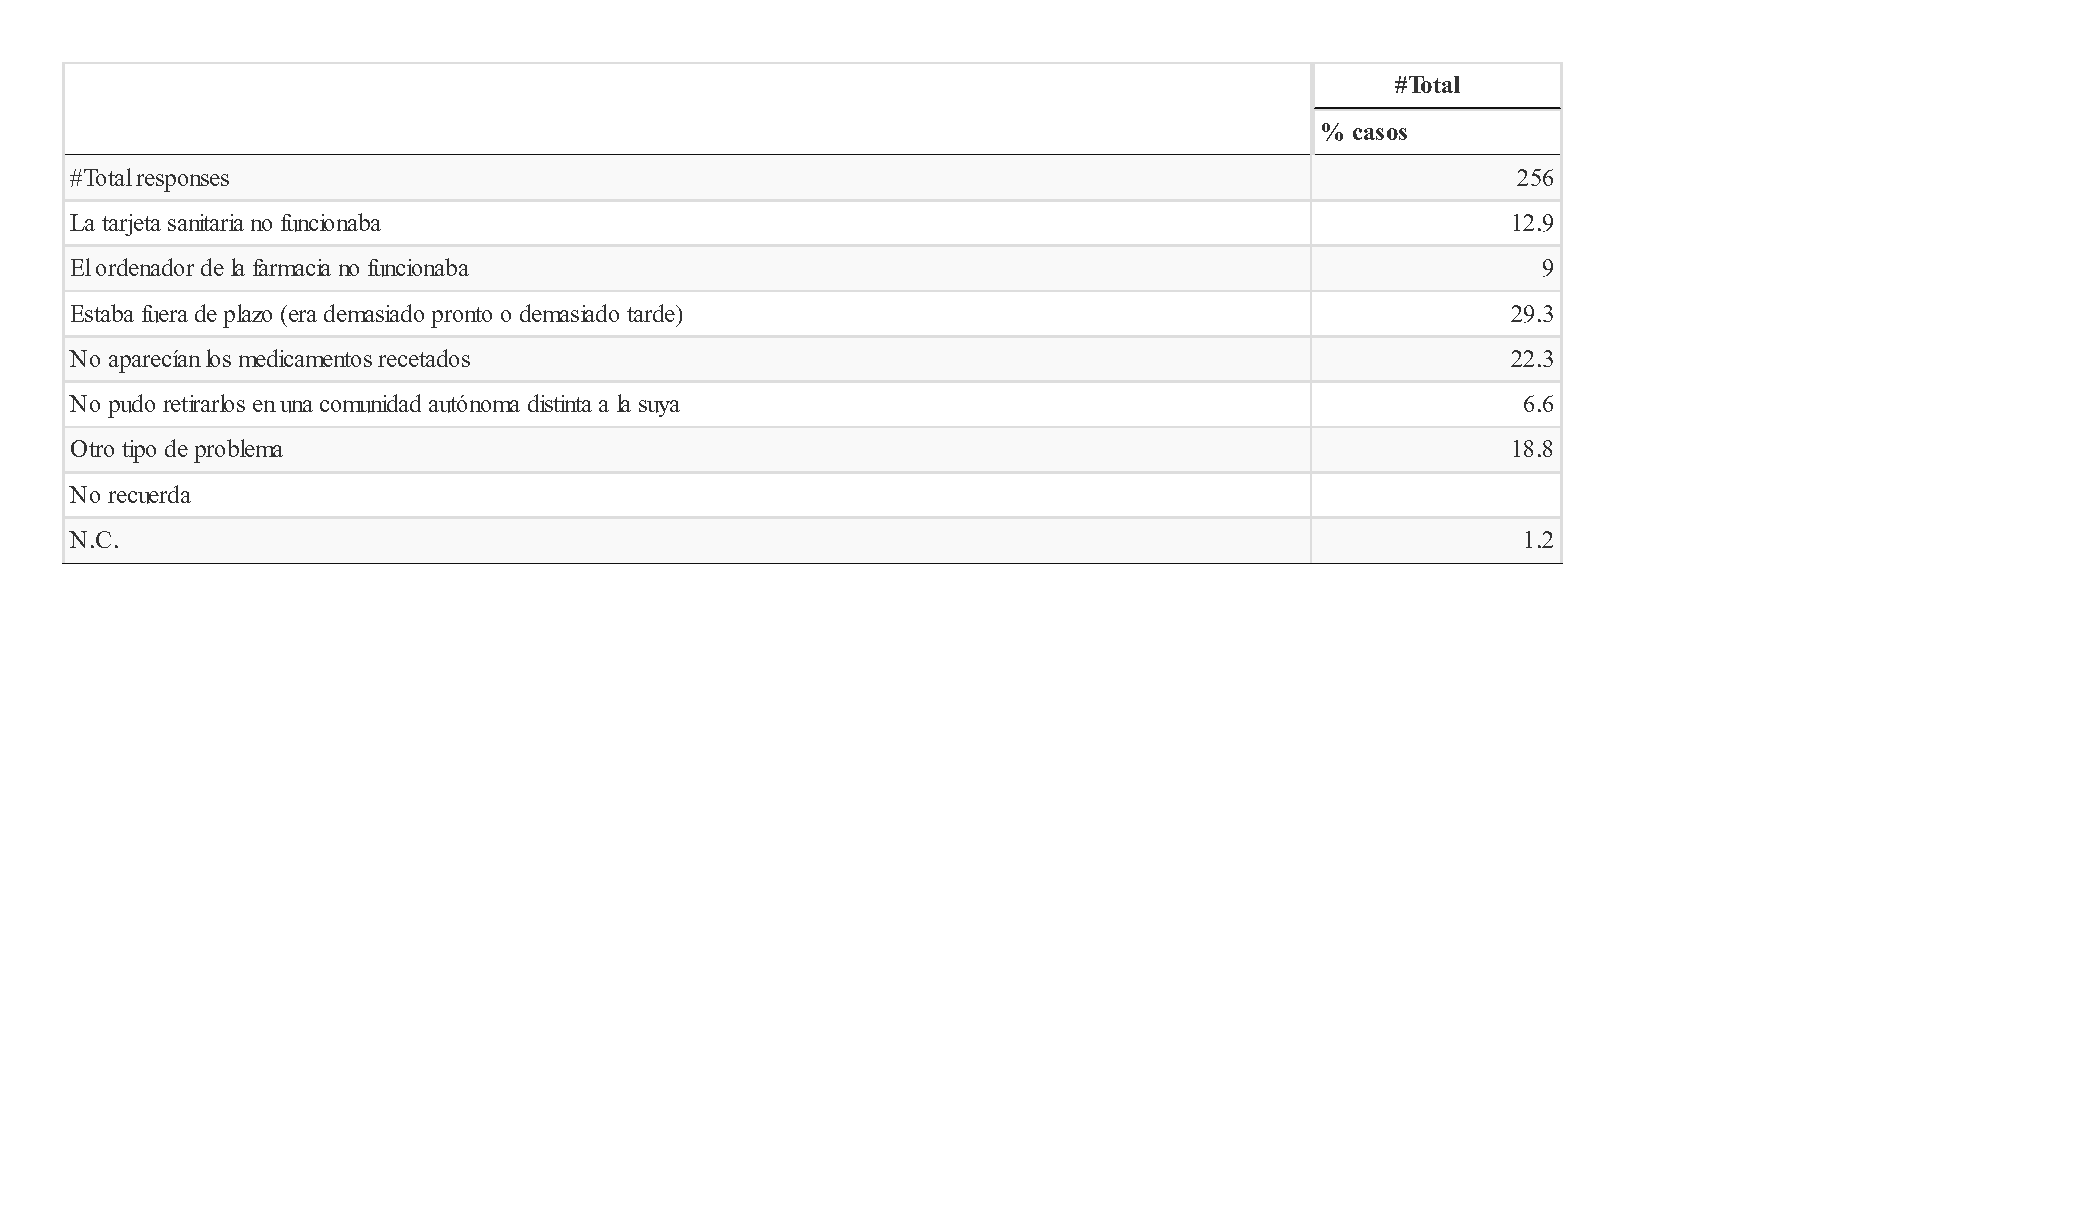
\includegraphics[width=0.95\linewidth]{Tablas-y-graficos-con-R-y-RStudio_files/figure-latex/unnamed-chunk-14-1} 

}

\caption{Frecuencias de P18}\label{fig:unnamed-chunk-14}
\end{figure}

\hypertarget{tablas-combinadas}{%
\subsection{Tablas combinadas}\label{tablas-combinadas}}

Con las múltiples también funciona el posicionamiento del estadístico casos -frecuencias- cuando combinamos los mismos (frecuencia y porcentaje) y podemos realizar las mismas variantes que antes.

Ubicar los cálculos dentro de las columnas \ldots{}

\begin{Shaded}
\begin{Highlighting}[]
\FunctionTok{as.datatable\_widget}\NormalTok{(data }\SpecialCharTok{\%\textgreater{}\%} 
  \FunctionTok{tab\_cells}\NormalTok{(}\FunctionTok{mdset\_f}\NormalTok{(P18C)) }\SpecialCharTok{\%\textgreater{}\%}  \CommentTok{\# o tab\_cells(mdset(P18C01 \%to\% P18C08))}
  \FunctionTok{tab\_stat\_cases}\NormalTok{(}\AttributeTok{label =}\StringTok{"Casos"}\NormalTok{) }\SpecialCharTok{\%\textgreater{}\%} 
  \FunctionTok{tab\_stat\_cpct}\NormalTok{(}\AttributeTok{label=}\StringTok{"\% casos"}\NormalTok{) }\SpecialCharTok{\%\textgreater{}\%} 
  \FunctionTok{tab\_stat\_cpct\_responses}\NormalTok{(}\AttributeTok{label=}\StringTok{"\% respuestas"}\NormalTok{) }\SpecialCharTok{\%\textgreater{}\%} 
  \FunctionTok{tab\_pivot}\NormalTok{(}\AttributeTok{stat\_position=}\StringTok{"inside\_columns"}\NormalTok{))}
\end{Highlighting}
\end{Shaded}

\begin{figure}[H]

{\centering 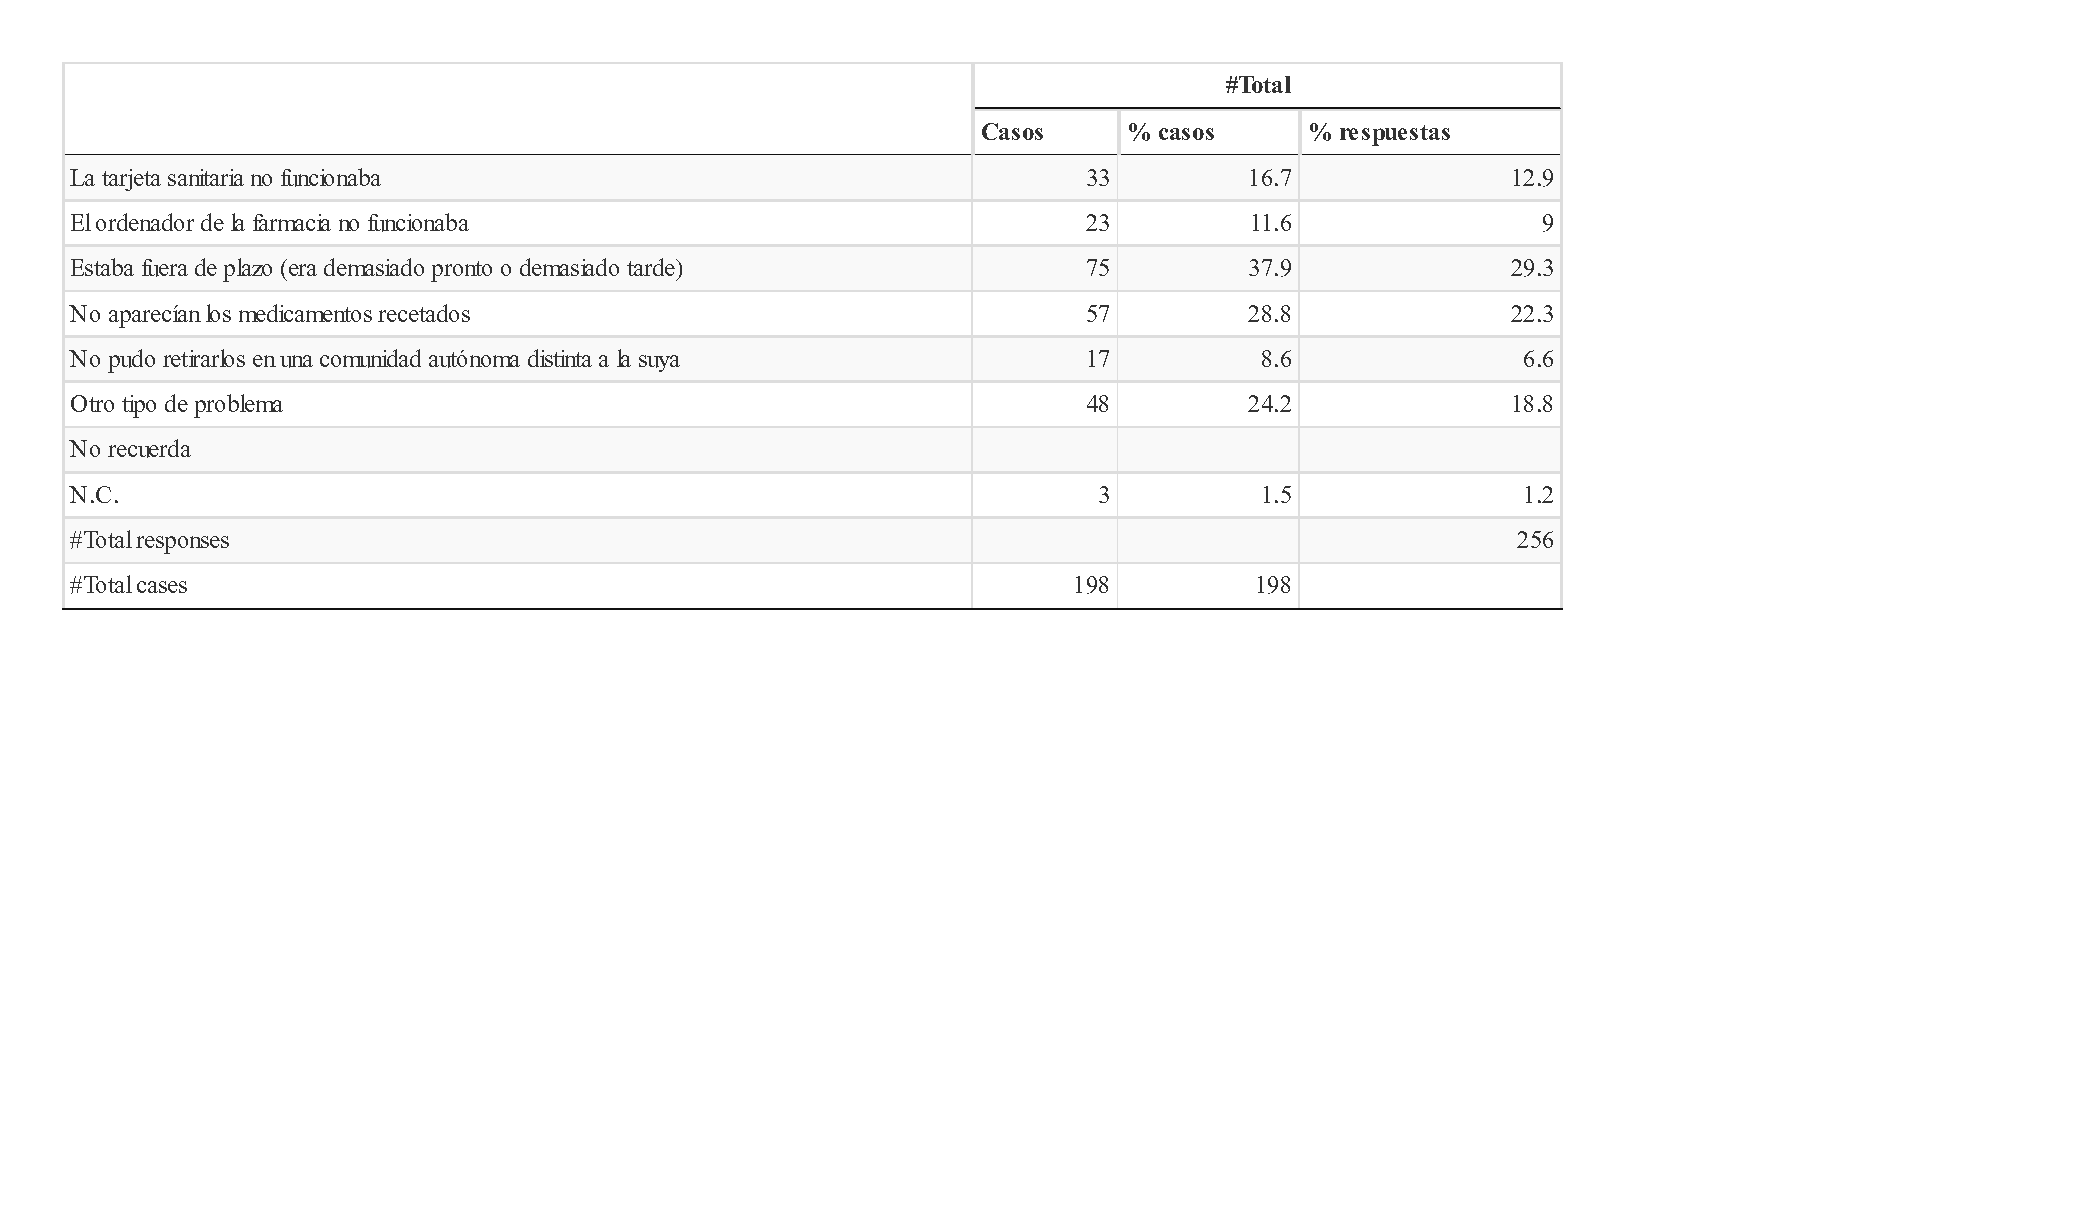
\includegraphics[width=0.95\linewidth]{Tablas-y-graficos-con-R-y-RStudio_files/figure-latex/unnamed-chunk-15-1} 

}

\caption{Frecuencias y porcentajes de P18 (1)}\label{fig:unnamed-chunk-15}
\end{figure}

Préstese atención a las dos líneas de \#Total, dado que las bases son diferentes (número de individuos y número de respuestas).

Podemos ubicar los cálculos dentro de las filas \ldots{}

\begin{Shaded}
\begin{Highlighting}[]
\FunctionTok{as.datatable\_widget}\NormalTok{(data }\SpecialCharTok{\%\textgreater{}\%} 
  \FunctionTok{tab\_cells}\NormalTok{(}\FunctionTok{mdset\_f}\NormalTok{(P18C)) }\SpecialCharTok{\%\textgreater{}\%}  \CommentTok{\# o tab\_cells(mdset(P18C01 \%to\% P18C08))}
  \FunctionTok{tab\_stat\_cases}\NormalTok{(}\AttributeTok{label =}\StringTok{"Casos"}\NormalTok{) }\SpecialCharTok{\%\textgreater{}\%} 
  \FunctionTok{tab\_stat\_cpct}\NormalTok{(}\AttributeTok{label=}\StringTok{"\% casos"}\NormalTok{) }\SpecialCharTok{\%\textgreater{}\%} 
  \FunctionTok{tab\_stat\_cpct\_responses}\NormalTok{(}\AttributeTok{label=}\StringTok{"\% respuestas"}\NormalTok{) }\SpecialCharTok{\%\textgreater{}\%} 
  \FunctionTok{tab\_pivot}\NormalTok{(}\AttributeTok{stat\_position=}\StringTok{"inside\_rows"}\NormalTok{))}
\end{Highlighting}
\end{Shaded}

\begin{figure}[H]

{\centering 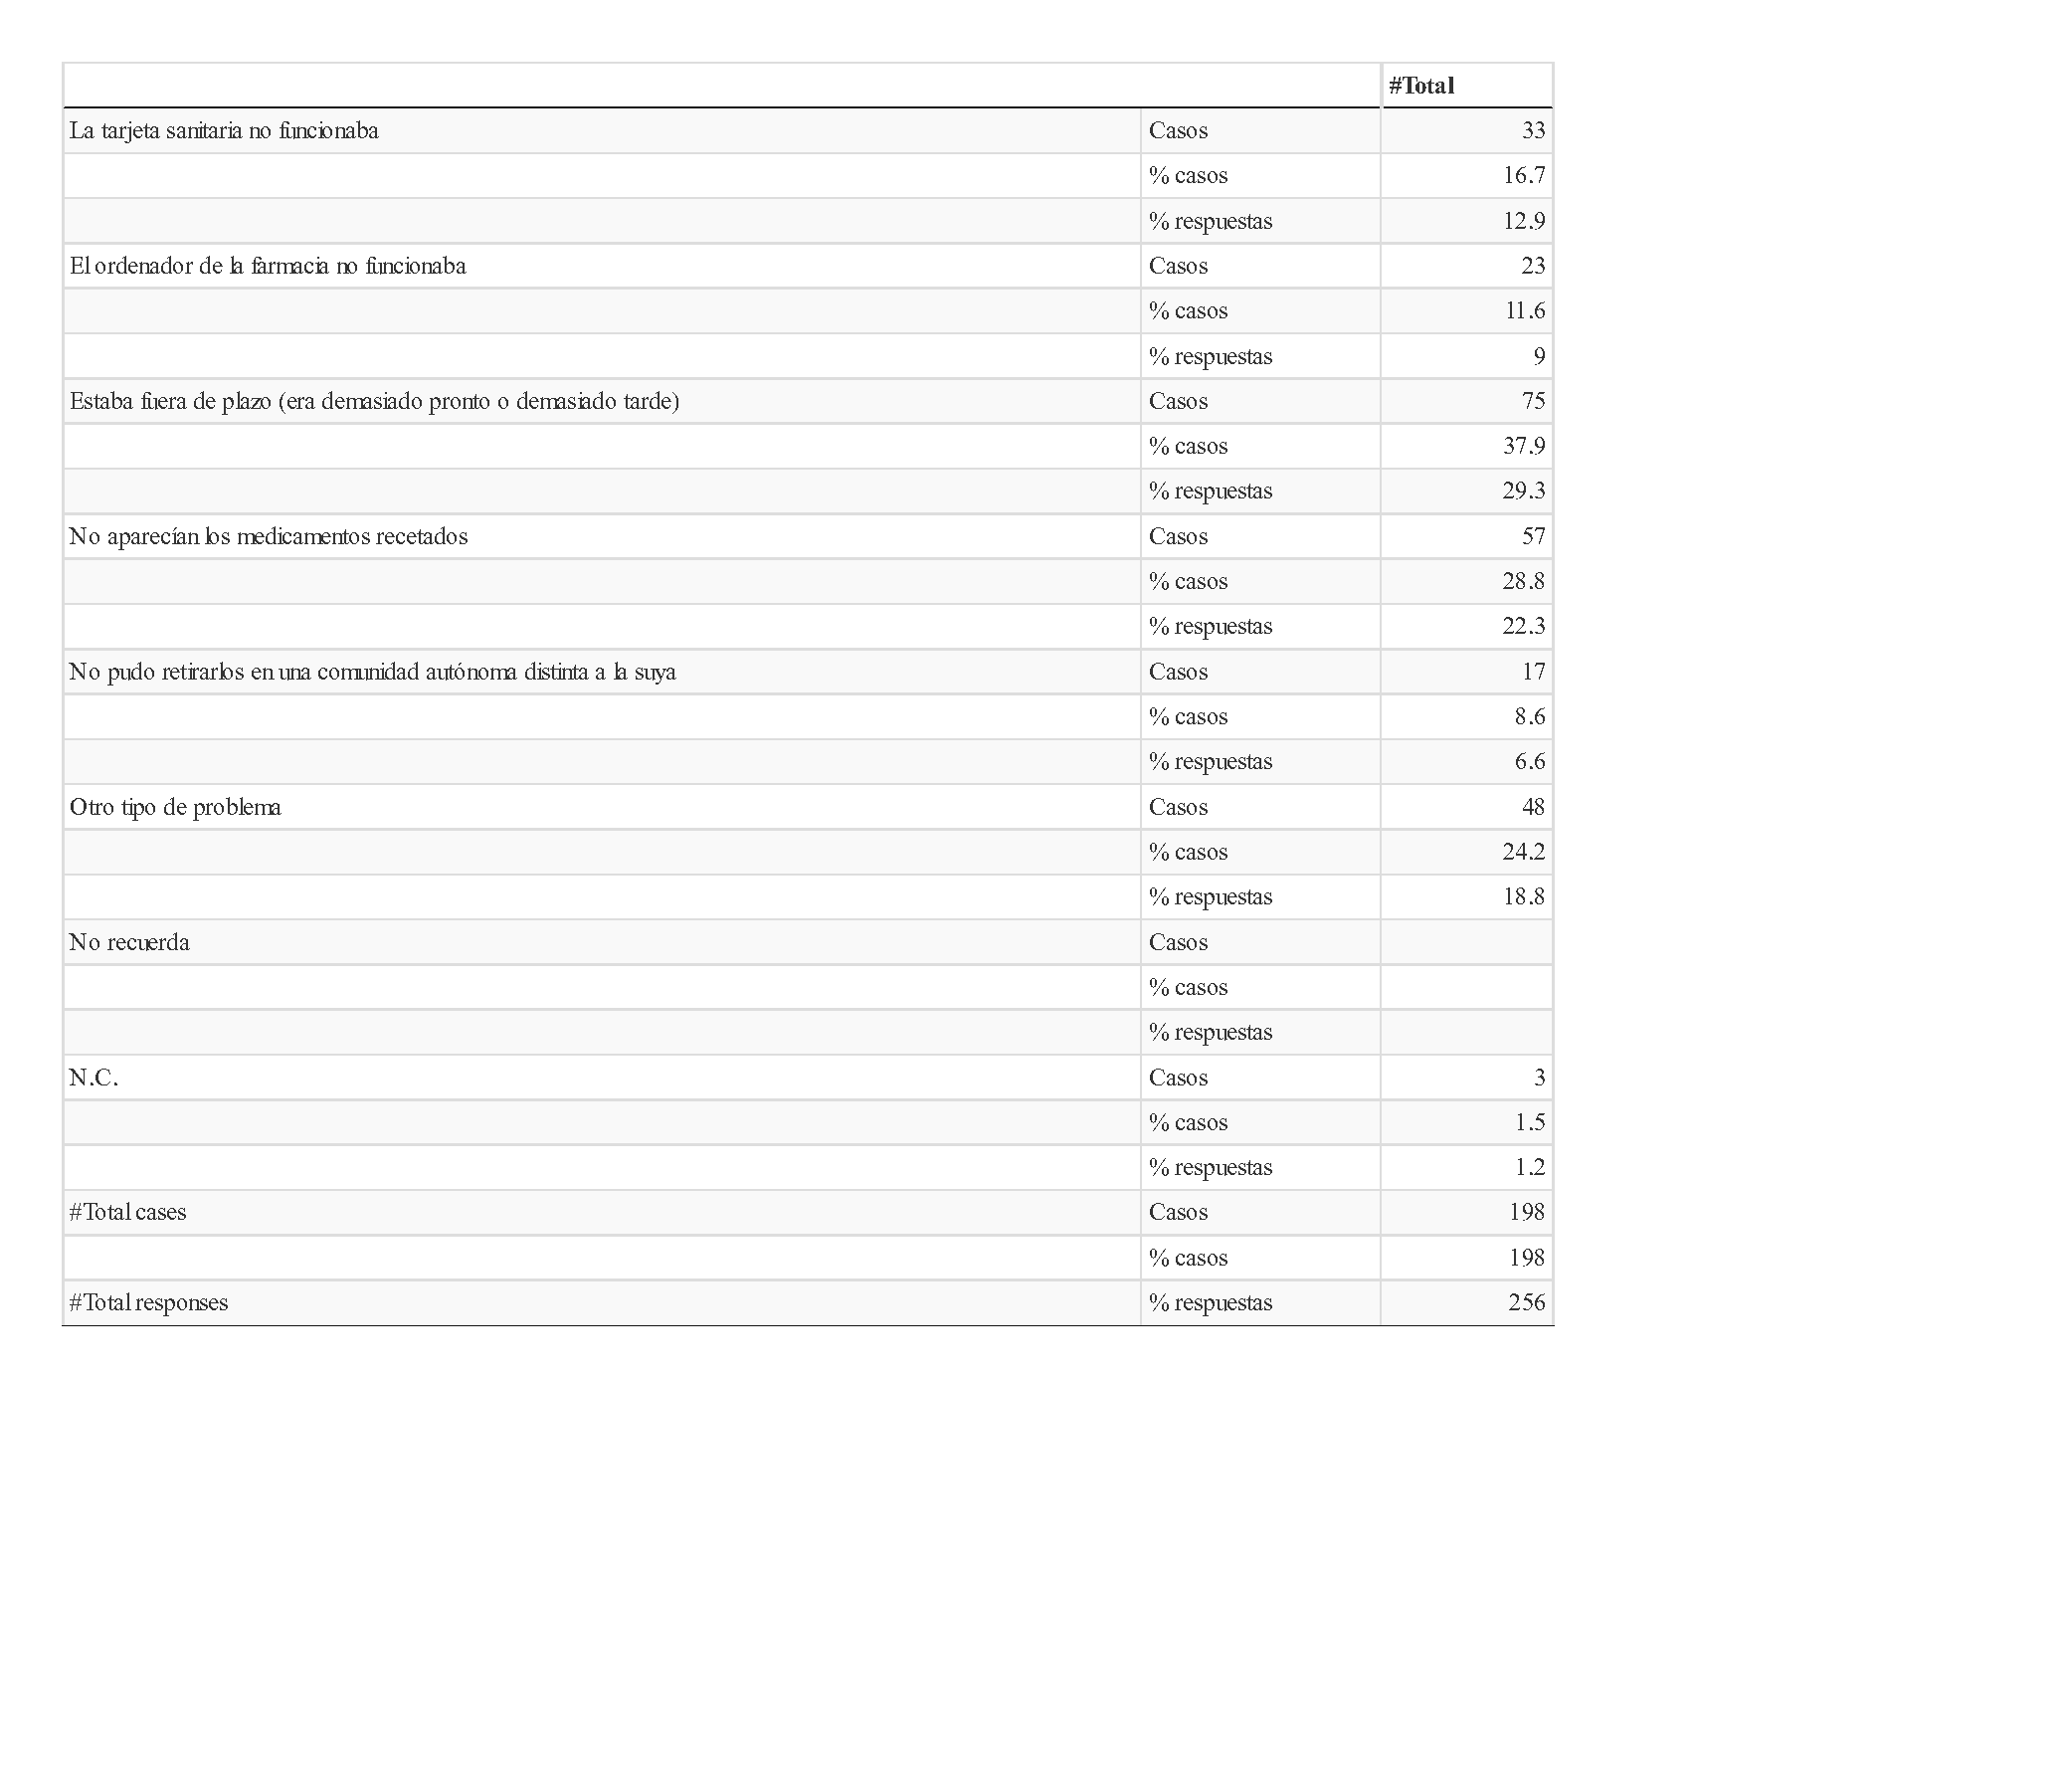
\includegraphics[width=0.95\linewidth]{Tablas-y-graficos-con-R-y-RStudio_files/figure-latex/unnamed-chunk-16-1} 

}

\caption{Frecuencias y porcentajes de P18 (2)}\label{fig:unnamed-chunk-16}
\end{figure}

Podemos ubicar los cálculos fuera de las columnas (igual a la anterior \texttt{inside...} porque no hay campo de columna) \ldots{}

\begin{Shaded}
\begin{Highlighting}[]
\FunctionTok{as.datatable\_widget}\NormalTok{(data }\SpecialCharTok{\%\textgreater{}\%} 
  \FunctionTok{tab\_cells}\NormalTok{(}\FunctionTok{mdset\_f}\NormalTok{(P18C)) }\SpecialCharTok{\%\textgreater{}\%}  \CommentTok{\# o tab\_cells(mdset(P18C01 \%to\% P18C08))}
  \FunctionTok{tab\_stat\_cases}\NormalTok{(}\AttributeTok{label =}\StringTok{"Casos"}\NormalTok{) }\SpecialCharTok{\%\textgreater{}\%} 
  \FunctionTok{tab\_stat\_cpct}\NormalTok{(}\AttributeTok{label=}\StringTok{"\% casos"}\NormalTok{) }\SpecialCharTok{\%\textgreater{}\%} 
  \FunctionTok{tab\_stat\_cpct\_responses}\NormalTok{(}\AttributeTok{label=}\StringTok{"\% respuestas"}\NormalTok{) }\SpecialCharTok{\%\textgreater{}\%} 
  \FunctionTok{tab\_pivot}\NormalTok{(}\AttributeTok{stat\_position=}\StringTok{"outside\_columns"}\NormalTok{))}
\end{Highlighting}
\end{Shaded}

\begin{figure}[H]

{\centering 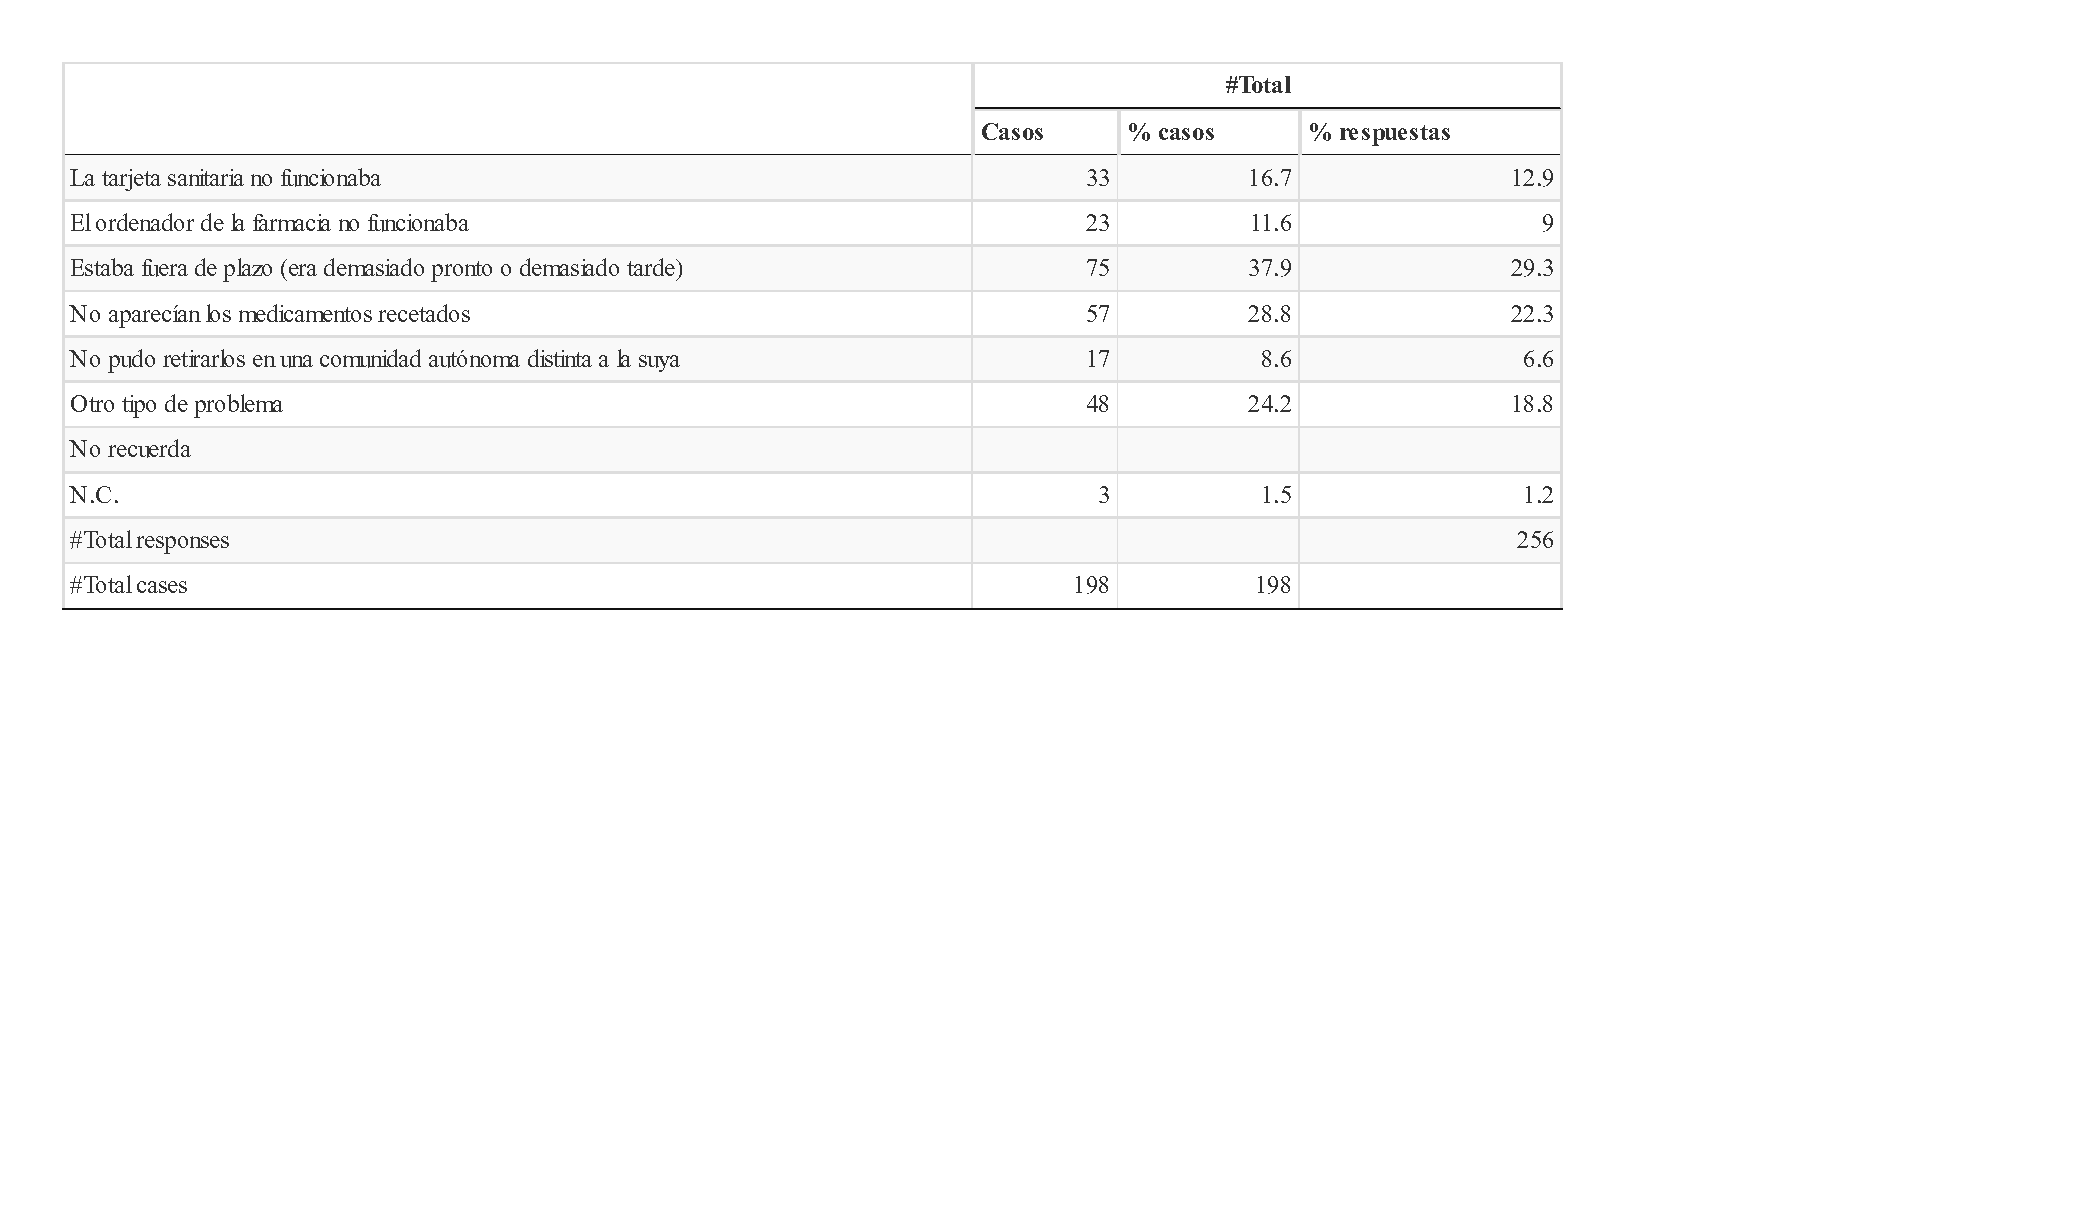
\includegraphics[width=0.95\linewidth]{Tablas-y-graficos-con-R-y-RStudio_files/figure-latex/unnamed-chunk-17-1} 

}

\caption{Frecuencias y porcentajes de P18 (3)}\label{fig:unnamed-chunk-17}
\end{figure}

Podemos ubicar los cálculos fuera de las filas \ldots{} nótese que la agrupación es diferente a la anterior con \texttt{inside\_rows}

\begin{Shaded}
\begin{Highlighting}[]
\FunctionTok{as.datatable\_widget}\NormalTok{(data }\SpecialCharTok{\%\textgreater{}\%} 
  \FunctionTok{tab\_cells}\NormalTok{(}\FunctionTok{mdset\_f}\NormalTok{(P18C)) }\SpecialCharTok{\%\textgreater{}\%}  \CommentTok{\# o tab\_cells(mdset(P18C01 \%to\% P18C08))}
  \FunctionTok{tab\_stat\_cases}\NormalTok{(}\AttributeTok{label =}\StringTok{"Casos"}\NormalTok{) }\SpecialCharTok{\%\textgreater{}\%} 
  \FunctionTok{tab\_stat\_cpct}\NormalTok{(}\AttributeTok{label=}\StringTok{"\% casos"}\NormalTok{) }\SpecialCharTok{\%\textgreater{}\%} 
  \FunctionTok{tab\_stat\_cpct\_responses}\NormalTok{(}\AttributeTok{label=}\StringTok{"\% respuestas"}\NormalTok{) }\SpecialCharTok{\%\textgreater{}\%} 
  \FunctionTok{tab\_pivot}\NormalTok{(}\AttributeTok{stat\_position=}\StringTok{"outside\_rows"}\NormalTok{))}
\end{Highlighting}
\end{Shaded}

\begin{figure}[H]

{\centering 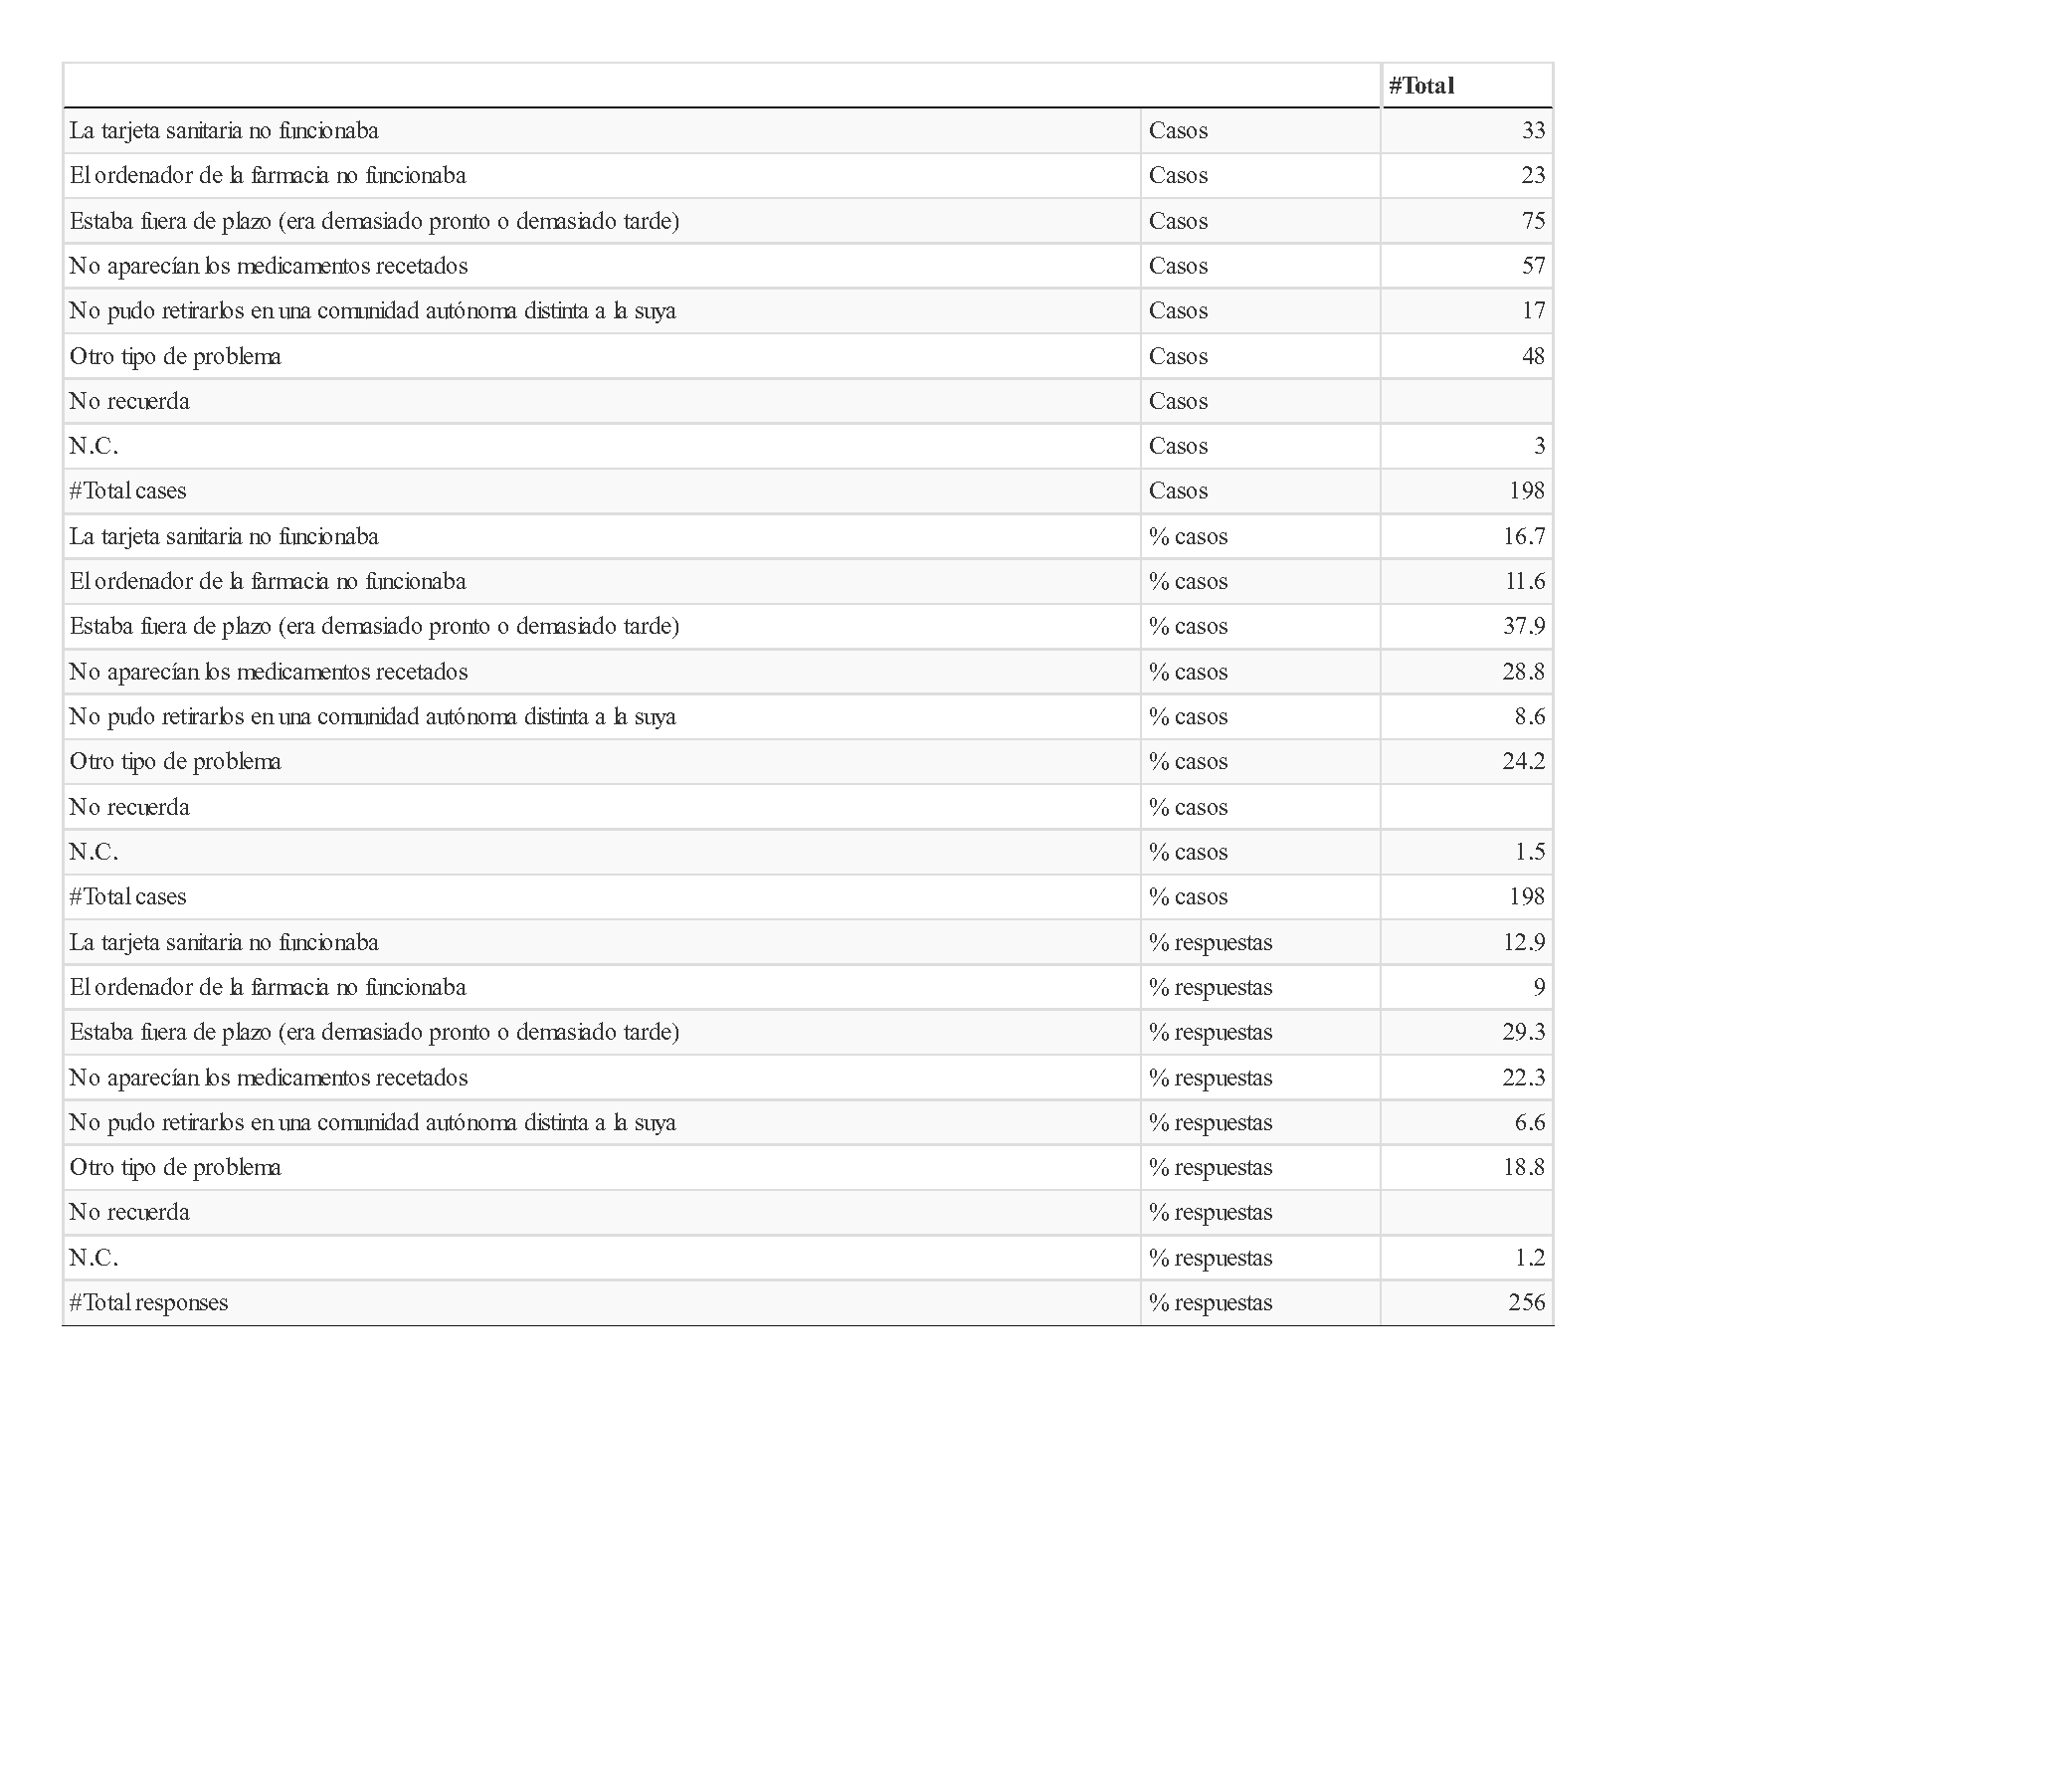
\includegraphics[width=0.95\linewidth]{Tablas-y-graficos-con-R-y-RStudio_files/figure-latex/unnamed-chunk-18-1} 

}

\caption{Frecuencias y porcentajes de P18 (4)}\label{fig:unnamed-chunk-18}
\end{figure}

\hypertarget{estaduxedsticos}{%
\section{Estadísticos}\label{estaduxedsticos}}

Hasta ahora hemos trabajado sólo con casos, pero ya hemos anticipado que al igual que con los recuentos de casos o frecuencias se puede trabajar con otros estadísticos como la suma, máximo, mínimo, media, mediana, error estándar y desviación típica. Vamos a ir viendo cómo se desarrollan estos cuadros.

\hypertarget{estaduxedsticos-buxe1sicos}{%
\subsection{Estadísticos básicos}\label{estaduxedsticos-buxe1sicos}}

Recordemos que hasta ahora no hemos cruzado la información, solo estamos trabajando con lo que se denomina medidas marginales.Nuestro primer ejemplo es un caso típico, donde queremos obtener la media (\texttt{tab\_stat\_mean}), la desviación típica (\texttt{tab\_stat\_sd()}) y la base de cálculo, es decir el número de casos con valor (\texttt{tab\_stat\_valid\_n()}) para el cálculo.

Así, siguiendo la misma estructra de las tablas anteriores, redactamos el siguiente script:

\begin{Shaded}
\begin{Highlighting}[]
\FunctionTok{as.datatable\_widget}\NormalTok{(data }\SpecialCharTok{\%\textgreater{}\%}
  \FunctionTok{tab\_cells}\NormalTok{(P3) }\SpecialCharTok{\%\textgreater{}\%}
  \FunctionTok{tab\_stat\_mean}\NormalTok{() }\SpecialCharTok{\%\textgreater{}\%}
  \FunctionTok{tab\_stat\_sd}\NormalTok{() }\SpecialCharTok{\%\textgreater{}\%}
  \FunctionTok{tab\_stat\_valid\_n}\NormalTok{() }\SpecialCharTok{\%\textgreater{}\%}
  \FunctionTok{tab\_pivot}\NormalTok{())}
\end{Highlighting}
\end{Shaded}

\begin{figure}[H]

{\centering \includegraphics[width=0.95\linewidth]{Tablas-y-graficos-con-R-y-RStudio_files/figure-latex/unnamed-chunk-19-1} 

}

\caption{Estadísticos marginales de P3 (1)}\label{fig:unnamed-chunk-19}
\end{figure}

No, no tienes por qué ver los nombres de los estadísticos en lengua inglesa. También aquí podemos jugar con la etiqueta (label).

\begin{Shaded}
\begin{Highlighting}[]
\FunctionTok{as.datatable\_widget}\NormalTok{(data }\SpecialCharTok{\%\textgreater{}\%}
  \FunctionTok{tab\_cells}\NormalTok{(P3) }\SpecialCharTok{\%\textgreater{}\%}
  \FunctionTok{tab\_stat\_mean}\NormalTok{(}\AttributeTok{label =} \StringTok{"media"}\NormalTok{) }\SpecialCharTok{\%\textgreater{}\%}
  \FunctionTok{tab\_stat\_sd}\NormalTok{(}\AttributeTok{label =} \StringTok{"desviación"}\NormalTok{) }\SpecialCharTok{\%\textgreater{}\%}
  \FunctionTok{tab\_stat\_valid\_n}\NormalTok{(}\AttributeTok{label =} \StringTok{"casos"}\NormalTok{) }\SpecialCharTok{\%\textgreater{}\%}
  \FunctionTok{tab\_pivot}\NormalTok{())}
\end{Highlighting}
\end{Shaded}

\begin{figure}[H]

{\centering \includegraphics[width=0.95\linewidth]{Tablas-y-graficos-con-R-y-RStudio_files/figure-latex/unnamed-chunk-20-1} 

}

\caption{Estadísticos marginales de P3 (2)}\label{fig:unnamed-chunk-20}
\end{figure}

Hagamos una nueva tabla con una pequeña variación, ahora vamos a poner los estadísticos en columnas.

\begin{Shaded}
\begin{Highlighting}[]
\FunctionTok{as.datatable\_widget}\NormalTok{(data }\SpecialCharTok{\%\textgreater{}\%}
  \FunctionTok{tab\_cells}\NormalTok{(P3) }\SpecialCharTok{\%\textgreater{}\%}
  \FunctionTok{tab\_stat\_mean}\NormalTok{(}\AttributeTok{label =} \StringTok{"media"}\NormalTok{) }\SpecialCharTok{\%\textgreater{}\%}
  \FunctionTok{tab\_stat\_sd}\NormalTok{(}\AttributeTok{label =} \StringTok{"desviación"}\NormalTok{) }\SpecialCharTok{\%\textgreater{}\%}
  \FunctionTok{tab\_stat\_valid\_n}\NormalTok{(}\AttributeTok{label =} \StringTok{"casos"}\NormalTok{) }\SpecialCharTok{\%\textgreater{}\%}
  \FunctionTok{tab\_pivot}\NormalTok{(}\AttributeTok{stat\_position =} \StringTok{"inside\_columns"}\NormalTok{))}
\end{Highlighting}
\end{Shaded}

\begin{figure}[H]

{\centering \includegraphics[width=0.95\linewidth]{Tablas-y-graficos-con-R-y-RStudio_files/figure-latex/unnamed-chunk-21-1} 

}

\caption{Estadísticos marginales de P3 (3)}\label{fig:unnamed-chunk-21}
\end{figure}

\texttt{expss} tiene además la posibilidad de obtener estos tres cálculos, bastante habituales por cierto, con un solo comando: \texttt{tab\_stat\_mean\_sd\_n()} pudiendo añadir además etiquetas separadas.

\begin{Shaded}
\begin{Highlighting}[]
\FunctionTok{as.datatable\_widget}\NormalTok{(data }\SpecialCharTok{\%\textgreater{}\%}
  \FunctionTok{tab\_cells}\NormalTok{(P3) }\SpecialCharTok{\%\textgreater{}\%}
  \FunctionTok{tab\_stat\_mean\_sd\_n}\NormalTok{(}\AttributeTok{labels =} \FunctionTok{c}\NormalTok{(}\StringTok{"media"}\NormalTok{, }\StringTok{"desviación"}\NormalTok{,}
    \StringTok{"casos"}\NormalTok{)) }\SpecialCharTok{\%\textgreater{}\%}
  \FunctionTok{tab\_pivot}\NormalTok{())}
\end{Highlighting}
\end{Shaded}

\begin{figure}[H]

{\centering \includegraphics[width=0.95\linewidth]{Tablas-y-graficos-con-R-y-RStudio_files/figure-latex/unnamed-chunk-22-1} 

}

\caption{Estadísticos marginales de P3 (4)}\label{fig:unnamed-chunk-22}
\end{figure}

\hypertarget{otros-estaduxedsticos}{%
\subsection{Otros estadísticos}\label{otros-estaduxedsticos}}

Además de los estadísticos más básicos, otros que podemos añadir son el máximo, el mínimo, la mediana, el error estándar y la suma. Los unimos todos.

\begin{Shaded}
\begin{Highlighting}[]
\FunctionTok{as.datatable\_widget}\NormalTok{(data }\SpecialCharTok{\%\textgreater{}\%}
  \FunctionTok{tab\_cells}\NormalTok{(P3) }\SpecialCharTok{\%\textgreater{}\%}
  \FunctionTok{tab\_stat\_mean}\NormalTok{(}\AttributeTok{label =} \StringTok{"Media"}\NormalTok{) }\SpecialCharTok{\%\textgreater{}\%}
  \FunctionTok{tab\_stat\_sd}\NormalTok{(}\AttributeTok{label =} \StringTok{"Desviación"}\NormalTok{) }\SpecialCharTok{\%\textgreater{}\%}
  \FunctionTok{tab\_stat\_max}\NormalTok{(}\AttributeTok{label =} \StringTok{"Máximo"}\NormalTok{) }\SpecialCharTok{\%\textgreater{}\%}
  \FunctionTok{tab\_stat\_min}\NormalTok{(}\AttributeTok{label =} \StringTok{"Mínimo"}\NormalTok{) }\SpecialCharTok{\%\textgreater{}\%}
  \FunctionTok{tab\_stat\_median}\NormalTok{(}\AttributeTok{label =} \StringTok{"Mediana"}\NormalTok{) }\SpecialCharTok{\%\textgreater{}\%}
  \FunctionTok{tab\_stat\_se}\NormalTok{(}\AttributeTok{label =} \StringTok{"Error estándar"}\NormalTok{) }\SpecialCharTok{\%\textgreater{}\%}
  \FunctionTok{tab\_stat\_sum}\NormalTok{(}\AttributeTok{label =} \StringTok{"Suma"}\NormalTok{) }\SpecialCharTok{\%\textgreater{}\%}
  \FunctionTok{tab\_pivot}\NormalTok{())}
\end{Highlighting}
\end{Shaded}

\begin{figure}[H]

{\centering \includegraphics[width=0.95\linewidth]{Tablas-y-graficos-con-R-y-RStudio_files/figure-latex/unnamed-chunk-23-1} 

}

\caption{Estadísticos marginales de P3 (5)}\label{fig:unnamed-chunk-23}
\end{figure}

Nótese que no se han definido ni filas, ni columnas. Es el modificador de la posición de los estadísticos (stat\_position) el que habilita la posición en una fila.

Del mismo modo, estos estadísticos pueden ubicarse en las columnas.

\begin{Shaded}
\begin{Highlighting}[]
\FunctionTok{as.datatable\_widget}\NormalTok{(data }\SpecialCharTok{\%\textgreater{}\%}
  \FunctionTok{tab\_cells}\NormalTok{(P3) }\SpecialCharTok{\%\textgreater{}\%}
  \FunctionTok{tab\_stat\_mean}\NormalTok{(}\AttributeTok{label =} \StringTok{"Media"}\NormalTok{) }\SpecialCharTok{\%\textgreater{}\%}
  \FunctionTok{tab\_stat\_sd}\NormalTok{(}\AttributeTok{label =} \StringTok{"Desviación"}\NormalTok{) }\SpecialCharTok{\%\textgreater{}\%}
  \FunctionTok{tab\_stat\_max}\NormalTok{(}\AttributeTok{label =} \StringTok{"Máximo"}\NormalTok{) }\SpecialCharTok{\%\textgreater{}\%}
  \FunctionTok{tab\_stat\_min}\NormalTok{(}\AttributeTok{label =} \StringTok{"Mínimo"}\NormalTok{) }\SpecialCharTok{\%\textgreater{}\%}
  \FunctionTok{tab\_stat\_median}\NormalTok{(}\AttributeTok{label =} \StringTok{"Mediana"}\NormalTok{) }\SpecialCharTok{\%\textgreater{}\%}
  \FunctionTok{tab\_stat\_se}\NormalTok{(}\AttributeTok{label =} \StringTok{"Error estándar"}\NormalTok{) }\SpecialCharTok{\%\textgreater{}\%}
  \FunctionTok{tab\_stat\_sum}\NormalTok{(}\AttributeTok{label =} \StringTok{"Suma"}\NormalTok{) }\SpecialCharTok{\%\textgreater{}\%}
  \FunctionTok{tab\_stat\_cases}\NormalTok{(}\AttributeTok{label =} \StringTok{"casos"}\NormalTok{) }\SpecialCharTok{\%\textgreater{}\%}
  \FunctionTok{tab\_pivot}\NormalTok{(}\AttributeTok{stat\_position =} \StringTok{"inside\_rows"}\NormalTok{))}
\end{Highlighting}
\end{Shaded}

\begin{figure}[H]

{\centering \includegraphics[width=0.95\linewidth]{Tablas-y-graficos-con-R-y-RStudio_files/figure-latex/unnamed-chunk-24-1} 

}

\caption{Estadísticos marginales de P3 (6)}\label{fig:unnamed-chunk-24}
\end{figure}

Hagamos finalmente una leve variación. Nótese que al utilizar \texttt{"\textbar{}"} en la etiqueta del estadístico casos, hemos eliminado la columna intermedia y aparace todo como más compacto. Este será un recurso que utilizaremos en muchas ocasiones.

\begin{Shaded}
\begin{Highlighting}[]
\FunctionTok{as.datatable\_widget}\NormalTok{(data }\SpecialCharTok{\%\textgreater{}\%}
  \FunctionTok{tab\_cells}\NormalTok{(P3) }\SpecialCharTok{\%\textgreater{}\%}
  \FunctionTok{tab\_stat\_mean}\NormalTok{(}\AttributeTok{label =} \StringTok{"Media"}\NormalTok{) }\SpecialCharTok{\%\textgreater{}\%}
  \FunctionTok{tab\_stat\_sd}\NormalTok{(}\AttributeTok{label =} \StringTok{"Desviación"}\NormalTok{) }\SpecialCharTok{\%\textgreater{}\%}
  \FunctionTok{tab\_stat\_max}\NormalTok{(}\AttributeTok{label =} \StringTok{"Máximo"}\NormalTok{) }\SpecialCharTok{\%\textgreater{}\%}
  \FunctionTok{tab\_stat\_min}\NormalTok{(}\AttributeTok{label =} \StringTok{"Mínimo"}\NormalTok{) }\SpecialCharTok{\%\textgreater{}\%}
  \FunctionTok{tab\_stat\_median}\NormalTok{(}\AttributeTok{label =} \StringTok{"Mediana"}\NormalTok{) }\SpecialCharTok{\%\textgreater{}\%}
  \FunctionTok{tab\_stat\_se}\NormalTok{(}\AttributeTok{label =} \StringTok{"Error estándar"}\NormalTok{) }\SpecialCharTok{\%\textgreater{}\%}
  \FunctionTok{tab\_stat\_sum}\NormalTok{(}\AttributeTok{label =} \StringTok{"Suma"}\NormalTok{) }\SpecialCharTok{\%\textgreater{}\%}
  \FunctionTok{tab\_stat\_cases}\NormalTok{(}\AttributeTok{label =} \StringTok{"|"}\NormalTok{) }\SpecialCharTok{\%\textgreater{}\%}
  \FunctionTok{tab\_pivot}\NormalTok{(}\AttributeTok{stat\_position =} \StringTok{"inside\_rows"}\NormalTok{))}
\end{Highlighting}
\end{Shaded}

\begin{figure}[H]

{\centering \includegraphics[width=0.95\linewidth]{Tablas-y-graficos-con-R-y-RStudio_files/figure-latex/unnamed-chunk-25-1} 

}

\caption{Estadísticos marginales de P3 (7)}\label{fig:unnamed-chunk-25}
\end{figure}

\hypertarget{conclusiuxf3n-1}{%
\section{Conclusión}\label{conclusiuxf3n-1}}

Creo que esta primera muestra de cómo procesar nuestra tabla de una única variable, es más que suficiente para colmar las expectativas más exigentes. Para aquellos que conozcan un poco más el funcionamiento de R, indicar que cada una de estas tablas, se puede almacenar como objeto sobre el que se puede trabajar. Este objeto es del tipo \texttt{etable} pero en el fondo es un objeto de tipo \texttt{\_dataframe\_} que por tanto puedes ser trabajado con comandos R estándar. Es de esta posibilidad de ser un \emph{dataframe} de donde deriva su capacidad de integración con otros paquetes como por ejemplo \texttt{highcharter} \citet{highcharter} que será uno de nuestros paquetes de referencia para gráficos. Para una presentación completa, véase la sección \ref{tse08} para una presentación de gráficos a partir de \texttt{\_dataframe\_} o de tablas cruzadas - \texttt{\_crosstab\_} -.

Hasta llegar ese momento, ahora en la siguiente sección \ref{tse04} analizamos las tablas cruzadas.

\hypertarget{tse04}{%
\chapter{Tablas cruzadas}\label{tse04}}

A diferencia de lo visto en la sección \ref{tse03}, en este epígrafe analizaremos como obtener cuadros resumen en los que existen variables en la cabecera, que determinan grupos o perfiles de análisis y existen variables en las filas, de las cuáles queremos conocer cómo se distribuyen sus alternativas de respuesta entre los diferentes perfiles o grupos que determinan las variables de columna. Al igual que sucedió con las tablas marginales, mostraremos poco a poco como trabajar con variables de respuesta simple, múltiple o con medidas estadísticas. Vamos a utilizar otros campos que se localizan en la base de datos del CIS (P3, P21A01, P21A02, P21A03, P31, P33). Aquí su resumen\ldots{} -nótese que se ha incluido la función \texttt{suppressMessages()} para no publicar los mensajes de carga del paquete y datos-.

\begin{Shaded}
\begin{Highlighting}[]
\FunctionTok{suppressMessages}\NormalTok{(}\FunctionTok{setwd}\NormalTok{(}\StringTok{"\textasciitilde{}/R/r{-}projects/00.tables"}\NormalTok{))  }\CommentTok{\#esta es la carpeta donde almacené el archivo (en una subcarpeta llamada data)}
\FunctionTok{suppressMessages}\NormalTok{(}\FunctionTok{library}\NormalTok{(expss))  }\CommentTok{\#cargamos el paquete}
\FunctionTok{suppressMessages}\NormalTok{(data }\OtherTok{\textless{}{-}} \FunctionTok{read\_spss}\NormalTok{(}\StringTok{"data/3192.sav"}\NormalTok{))  }\CommentTok{\#cargamos los datos}
\NormalTok{data}\SpecialCharTok{$}\NormalTok{P3}
\end{Highlighting}
\end{Shaded}

\begin{verbatim}
## LABEL: Escala de satisfacción (1-10) con el funcionamiento del sistema sanitario español 
## VALUES:
## 6, 7, 8, 8, 7, 5, 7, 7, 8, 7, 7, 6, 6, 7, 7, 6, 5, 8, 7, 7, 8, 10, 8, 6, 6, 9, 8, 8, 7, 6, 9, 6, 8, 8, 6, 7, 7, 5, 8, 6, 6, 8, 4, 4, 5, 7, 7, 8, 10, 7... 50 items printed out of 2557 
## VALUE LABELS:                        
##   1 1 Muy insatisfecho/a
##   2 2                   
##   3 3                   
##   4 4                   
##   5 5                   
##   6 6                   
##   7 7                   
##   8 8                   
##   9 9                   
##  10 10 Muy satisfecho/a 
##  98 N.S.                
##  99 N.C.
\end{verbatim}

\begin{Shaded}
\begin{Highlighting}[]
\NormalTok{data}\SpecialCharTok{$}\NormalTok{P21A01}
\end{Highlighting}
\end{Shaded}

\begin{verbatim}
## LABEL: Medicamentos que recetan por adelantado (para que no falten) 
## VALUES:
## 0, 0, 0, 0, 0, 0, NA, 0, 0, 0, 0, 0, 0, 0, 0, 0, NA, 0, NA, 0, 0, NA, 0, 0, 0, 0, 0, 0, 0, 0, 0, 0, 0, 0, 0, 1, 0, 0, 1, 0, 0, 0, 0, 0, 0, 0, 0, 0, 0, 0... 50 items printed out of 2557 
## VALUE LABELS:           
##  0 N.P.    
##  1 Menciona
\end{verbatim}

\begin{Shaded}
\begin{Highlighting}[]
\NormalTok{data}\SpecialCharTok{$}\NormalTok{P21A02}
\end{Highlighting}
\end{Shaded}

\begin{verbatim}
## LABEL: Envases que han quedado sin usar porque cambiaron el tratamiento 
## VALUES:
## 0, 0, 0, 0, 0, 0, NA, 0, 0, 0, 0, 0, 0, 0, 0, 0, 1, 0, NA, 0, 0, 1, 0, 0, 0, 0, 0, 0, 0, 0, 0, 0, 0, 0, 0, NA, 0, 0, NA, 0, 0, 0, 0, 0, 0, 0, 0, 0, 0, 0... 50 items printed out of 2557 
## VALUE LABELS:           
##  0 N.P.    
##  1 Menciona
\end{verbatim}

\begin{Shaded}
\begin{Highlighting}[]
\NormalTok{data}\SpecialCharTok{$}\NormalTok{P21A03}
\end{Highlighting}
\end{Shaded}

\begin{verbatim}
## LABEL: Medicamentos que decidió no tomar 
## VALUES:
## 0, 0, 0, 0, 0, 0, 1, 0, 0, 0, 0, 0, 0, 0, 0, 0, 1, 0, 1, 0, 0, NA, 0, 0, 0, 0, 0, 0, 0, 0, 0, 0, 0, 0, 0, NA, 0, 0, NA, 0, 0, 0, 0, 0, 0, 0, 0, 0, 0, 0... 50 items printed out of 2557 
## VALUE LABELS:           
##  0 N.P.    
##  1 Menciona
\end{verbatim}

\begin{Shaded}
\begin{Highlighting}[]
\NormalTok{data}\SpecialCharTok{$}\NormalTok{P31}
\end{Highlighting}
\end{Shaded}

\begin{verbatim}
## LABEL: Sexo de la persona entrevistada 
## VALUES:
## 2, 1, 2, 1, 2, 2, 1, 1, 2, 2, 1, 1, 2, 1, 2, 2, 2, 1, 2, 2, 2, 1, 2, 1, 1, 2, 1, 1, 2, 2, 1, 2, 1, 1, 1, 2, 2, 2, 1, 2, 1, 1, 2, 2, 1, 1, 1, 1, 2, 2... 50 items printed out of 2557 
## VALUE LABELS:         
##  1 Hombre
##  2 Mujer
\end{verbatim}

\begin{Shaded}
\begin{Highlighting}[]
\NormalTok{data}\SpecialCharTok{$}\NormalTok{P33}
\end{Highlighting}
\end{Shaded}

\begin{verbatim}
## LABEL: Estado civil de la persona entrevistada 
## VALUES:
## 1, 1, 1, 1, 3, 2, 2, 2, 1, 9, 1, 2, 1, 1, 3, 2, 3, 1, 1, 1, 1, 1, 1, 2, 2, 3, 2, 1, 1, 2, 2, 2, 1, 2, 1, 3, 1, 1, 1, 1, 5, 1, 1, 1, 1, 2, 5, 1, 5, 1... 50 items printed out of 2557 
## VALUE LABELS:               
##  1 Casado/a    
##  2 Soltero/a   
##  3 Viudo/a     
##  4 Separado/a  
##  5 Divorciado/a
##  9 N.C.
\end{verbatim}

\hypertarget{buxe1sica-con-variables-simples}{%
\section{Básica con variables simples}\label{buxe1sica-con-variables-simples}}

Las tablas que vamos a hacer a continuación, siempre son tablas en las que intervienen al menos dos variables. Una de las variables irá a columnas y la otra variable irá a filas. De ellas se calcularán las frecuencias absolutas o relativas y/o los estadísticos. Vamos a empezar sólo con el estadístico frecuencias, y posteriormente ya pasaremos a estadísticos como la media, suma, etc\ldots{}

\hypertarget{de-frecuencias-variable-simple-y-suxf3lo-absolutos}{%
\subsection{De frecuencias, variable simple y sólo absolutos}\label{de-frecuencias-variable-simple-y-suxf3lo-absolutos}}

Usaremos la variable P31 para las columnas, P33 en las celdas (de la que se hará el cálculo)y el estadístico a usar será el nº de casos.

\begin{Shaded}
\begin{Highlighting}[]
\FunctionTok{as.datatable\_widget}\NormalTok{(data }\SpecialCharTok{\%\textgreater{}\%}
  \FunctionTok{tab\_cells}\NormalTok{(P33) }\SpecialCharTok{\%\textgreater{}\%}
  \FunctionTok{tab\_cols}\NormalTok{(}\FunctionTok{total}\NormalTok{(), P31) }\SpecialCharTok{\%\textgreater{}\%}
  \FunctionTok{tab\_stat\_cases}\NormalTok{(}\AttributeTok{total\_row\_position =} \StringTok{"above"}\NormalTok{, }\AttributeTok{total\_label =} \StringTok{"Total"}\NormalTok{) }\SpecialCharTok{\%\textgreater{}\%}
  \FunctionTok{tab\_pivot}\NormalTok{())}
\end{Highlighting}
\end{Shaded}

\begin{figure}[H]

{\centering \includegraphics[width=0.95\linewidth]{Tablas-y-graficos-con-R-y-RStudio_files/figure-latex/unnamed-chunk-27-1} 

}

\caption{Cruce de estado civil por sexo}\label{fig:unnamed-chunk-27}
\end{figure}

\hypertarget{de-frecuencias-variable-simple-con-porcentajes-de-columna}{%
\subsection{De frecuencias, variable simple, con porcentajes de columna}\label{de-frecuencias-variable-simple-con-porcentajes-de-columna}}

Al igual que hicimos con las tablas marginales vamos a repetir esta tabla, pero en porcentaje de columna (vertical).

\begin{Shaded}
\begin{Highlighting}[]
\FunctionTok{as.datatable\_widget}\NormalTok{(data }\SpecialCharTok{\%\textgreater{}\%}
    \FunctionTok{tab\_cells}\NormalTok{(P33) }\SpecialCharTok{\%\textgreater{}\%}
    \FunctionTok{tab\_cols}\NormalTok{(}\FunctionTok{total}\NormalTok{(), P31) }\SpecialCharTok{\%\textgreater{}\%}
    \FunctionTok{tab\_stat\_cpct}\NormalTok{(}\AttributeTok{total\_row\_position =} \StringTok{"above"}\NormalTok{, }\AttributeTok{total\_label =} \StringTok{"Total"}\NormalTok{) }\SpecialCharTok{\%\textgreater{}\%} \CommentTok{\# aquí señalo los porcentajes de columna}
    \FunctionTok{tab\_pivot}\NormalTok{())}
\end{Highlighting}
\end{Shaded}

\begin{figure}[H]

{\centering \includegraphics[width=0.95\linewidth]{Tablas-y-graficos-con-R-y-RStudio_files/figure-latex/unnamed-chunk-28-1} 

}

\caption{Cruce de estado civil por sexo, porcentaje de columna}\label{fig:unnamed-chunk-28}
\end{figure}

\hypertarget{de-frecuencias-variable-simple-con-porcentajes-de-fila}{%
\subsection{De frecuencias, variable simple, con porcentajes de fila}\label{de-frecuencias-variable-simple-con-porcentajes-de-fila}}

Al igual que hicimos con las tablas marginales vamos a repetir esta tabla, pero en porcentaje de fila (horizontal).

\begin{Shaded}
\begin{Highlighting}[]
\FunctionTok{as.datatable\_widget}\NormalTok{(data }\SpecialCharTok{\%\textgreater{}\%}
    \FunctionTok{tab\_cells}\NormalTok{(P33) }\SpecialCharTok{\%\textgreater{}\%}
    \FunctionTok{tab\_cols}\NormalTok{(}\FunctionTok{total}\NormalTok{(), P31) }\SpecialCharTok{\%\textgreater{}\%}
    \FunctionTok{tab\_stat\_rpct}\NormalTok{(}\AttributeTok{total\_row\_position =} \StringTok{"above"}\NormalTok{, }\AttributeTok{total\_label =} \StringTok{"Total"}\NormalTok{) }\SpecialCharTok{\%\textgreater{}\%} \CommentTok{\# aquí señalo los porcentajes de fila}
    \FunctionTok{tab\_pivot}\NormalTok{())}
\end{Highlighting}
\end{Shaded}

\begin{figure}[H]

{\centering \includegraphics[width=0.95\linewidth]{Tablas-y-graficos-con-R-y-RStudio_files/figure-latex/unnamed-chunk-29-1} 

}

\caption{Cruce de estado civil por sexo, porcentaje de fila}\label{fig:unnamed-chunk-29}
\end{figure}

\hypertarget{de-frecuencias-variable-simple-con-porcentajes-total-muestra}{%
\subsection{De frecuencias, variable simple, con porcentajes total muestra}\label{de-frecuencias-variable-simple-con-porcentajes-total-muestra}}

Al igual que hicimos con las tablas marginales vamos a repetir esta tabla, pero en porcentaje sobre el total de la muestra.

\begin{Shaded}
\begin{Highlighting}[]
\FunctionTok{as.datatable\_widget}\NormalTok{(data }\SpecialCharTok{\%\textgreater{}\%}
    \FunctionTok{tab\_cells}\NormalTok{(P33) }\SpecialCharTok{\%\textgreater{}\%}
    \FunctionTok{tab\_cols}\NormalTok{(}\FunctionTok{total}\NormalTok{(), P31) }\SpecialCharTok{\%\textgreater{}\%}
    \FunctionTok{tab\_stat\_tpct}\NormalTok{(}\AttributeTok{total\_row\_position =} \StringTok{"above"}\NormalTok{, }\AttributeTok{total\_label =} \StringTok{"Total"}\NormalTok{) }\SpecialCharTok{\%\textgreater{}\%} \CommentTok{\# aquí señalo los porcentajes total muestra}
    \FunctionTok{tab\_pivot}\NormalTok{())}
\end{Highlighting}
\end{Shaded}

\begin{figure}[H]

{\centering \includegraphics[width=0.95\linewidth]{Tablas-y-graficos-con-R-y-RStudio_files/figure-latex/unnamed-chunk-30-1} 

}

\caption{Cruce de estado civil por sexo, porcentaje sobre el total de la muestra}\label{fig:unnamed-chunk-30}
\end{figure}

\hypertarget{combinaciones-de-los-anteriores}{%
\subsection{Combinaciones de los anteriores}\label{combinaciones-de-los-anteriores}}

Vamos ahora a hacer combinaciones entre ellos. Advierto que cada vez se dificulta más la tabla en su lectura. Como dije inicialmente, me decanto más por tablas sencillas y con un sólo dato.

\begin{Shaded}
\begin{Highlighting}[]
\FunctionTok{as.datatable\_widget}\NormalTok{(data }\SpecialCharTok{\%\textgreater{}\%}
  \FunctionTok{tab\_cells}\NormalTok{(P33) }\SpecialCharTok{\%\textgreater{}\%}
  \FunctionTok{tab\_cols}\NormalTok{(}\FunctionTok{total}\NormalTok{(), P31) }\SpecialCharTok{\%\textgreater{}\%}
  \FunctionTok{tab\_stat\_cases}\NormalTok{(}\AttributeTok{label =} \StringTok{"Casos"}\NormalTok{) }\SpecialCharTok{\%\textgreater{}\%}
  \FunctionTok{tab\_stat\_cpct}\NormalTok{(}\AttributeTok{label =} \StringTok{"\% casos"}\NormalTok{) }\SpecialCharTok{\%\textgreater{}\%}
  \FunctionTok{tab\_pivot}\NormalTok{(}\AttributeTok{stat\_position =} \StringTok{"inside\_columns"}\NormalTok{))}
\end{Highlighting}
\end{Shaded}

\begin{figure}[H]

{\centering \includegraphics[width=0.95\linewidth]{Tablas-y-graficos-con-R-y-RStudio_files/figure-latex/unnamed-chunk-31-1} 

}

\caption{Combinación de casos y porcentajes dentro de las columnas}\label{fig:unnamed-chunk-31}
\end{figure}

Y la misma tabla pero con los estadísticos en las filas combinando frecuencia y porcentaje\ldots{}

\begin{Shaded}
\begin{Highlighting}[]
\FunctionTok{as.datatable\_widget}\NormalTok{(data }\SpecialCharTok{\%\textgreater{}\%}
  \FunctionTok{tab\_cells}\NormalTok{(P33) }\SpecialCharTok{\%\textgreater{}\%}
  \FunctionTok{tab\_cols}\NormalTok{(}\FunctionTok{total}\NormalTok{(), P31) }\SpecialCharTok{\%\textgreater{}\%}
  \FunctionTok{tab\_stat\_cases}\NormalTok{(}\AttributeTok{label =} \StringTok{"Casos"}\NormalTok{) }\SpecialCharTok{\%\textgreater{}\%}
  \FunctionTok{tab\_stat\_cpct}\NormalTok{(}\AttributeTok{label =} \StringTok{"\% casos"}\NormalTok{) }\SpecialCharTok{\%\textgreater{}\%}
  \FunctionTok{tab\_pivot}\NormalTok{(}\AttributeTok{stat\_position =} \StringTok{"outside\_columns"}\NormalTok{))}
\end{Highlighting}
\end{Shaded}

\begin{figure}[H]

{\centering \includegraphics[width=0.95\linewidth]{Tablas-y-graficos-con-R-y-RStudio_files/figure-latex/unnamed-chunk-32-1} 

}

\caption{Combinación de casos y porcentajes por tipo de estadístico en columnas}\label{fig:unnamed-chunk-32}
\end{figure}

Y la misma tabla pero con los estadísticos en las filas combinando frecuencia y porcentaje\ldots{}

\begin{Shaded}
\begin{Highlighting}[]
\FunctionTok{as.datatable\_widget}\NormalTok{(data }\SpecialCharTok{\%\textgreater{}\%}
  \FunctionTok{tab\_cells}\NormalTok{(P33) }\SpecialCharTok{\%\textgreater{}\%}
  \FunctionTok{tab\_cols}\NormalTok{(}\FunctionTok{total}\NormalTok{(), P31) }\SpecialCharTok{\%\textgreater{}\%}
  \FunctionTok{tab\_stat\_cases}\NormalTok{(}\AttributeTok{label =} \StringTok{"Casos"}\NormalTok{) }\SpecialCharTok{\%\textgreater{}\%}
  \FunctionTok{tab\_stat\_cpct}\NormalTok{(}\AttributeTok{label =} \StringTok{"\% casos"}\NormalTok{) }\SpecialCharTok{\%\textgreater{}\%}
  \FunctionTok{tab\_pivot}\NormalTok{(}\AttributeTok{stat\_position =} \StringTok{"inside\_rows"}\NormalTok{))}
\end{Highlighting}
\end{Shaded}

\begin{figure}[H]

{\centering \includegraphics[width=0.95\linewidth]{Tablas-y-graficos-con-R-y-RStudio_files/figure-latex/unnamed-chunk-33-1} 

}

\caption{Combinación de casos y porcentajes dentro de las filas}\label{fig:unnamed-chunk-33}
\end{figure}

Y la misma tabla pero con los estadísticos en las filas por bloque de tipo de estadístico\ldots{}

\begin{Shaded}
\begin{Highlighting}[]
\FunctionTok{as.datatable\_widget}\NormalTok{(data }\SpecialCharTok{\%\textgreater{}\%}
  \FunctionTok{tab\_cells}\NormalTok{(P33) }\SpecialCharTok{\%\textgreater{}\%}
  \FunctionTok{tab\_cols}\NormalTok{(}\FunctionTok{total}\NormalTok{(), P31) }\SpecialCharTok{\%\textgreater{}\%}
  \FunctionTok{tab\_stat\_cases}\NormalTok{(}\AttributeTok{label =} \StringTok{"Casos"}\NormalTok{) }\SpecialCharTok{\%\textgreater{}\%}
  \FunctionTok{tab\_stat\_cpct}\NormalTok{(}\AttributeTok{label =} \StringTok{"\% casos"}\NormalTok{) }\SpecialCharTok{\%\textgreater{}\%}
  \FunctionTok{tab\_pivot}\NormalTok{(}\AttributeTok{stat\_position =} \StringTok{"outside\_rows"}\NormalTok{))}
\end{Highlighting}
\end{Shaded}

\begin{figure}[H]

{\centering \includegraphics[width=0.95\linewidth]{Tablas-y-graficos-con-R-y-RStudio_files/figure-latex/unnamed-chunk-34-1} 

}

\caption{Combinación de casos y porcentajes, por tipo de estadístico en filas}\label{fig:unnamed-chunk-34}
\end{figure}

\hypertarget{buxe1sica-con-muxfaltiples}{%
\section{Básica con múltiples}\label{buxe1sica-con-muxfaltiples}}

Vamos a realizar ahora el mismo conjunto de tablas, pero en las filas, en lugar de una variable de tipo simple, vamos a utilizar una variable de tipo múltiple. Repetimos los cruces pero cambiamos las celdas donde ahora usaremos la variable P21A con la instrucción \texttt{tab\_cells(mdset(P21A01\ \%to\%\ P21A03))}.

\hypertarget{de-frecuencias-variable-muxfaltiple-y-suxf3lo-absolutos}{%
\subsection{De frecuencias, variable múltiple y sólo absolutos}\label{de-frecuencias-variable-muxfaltiple-y-suxf3lo-absolutos}}

\begin{Shaded}
\begin{Highlighting}[]
\FunctionTok{as.datatable\_widget}\NormalTok{(data }\SpecialCharTok{\%\textgreater{}\%}
  \FunctionTok{tab\_cells}\NormalTok{(}\FunctionTok{mdset}\NormalTok{(P21A01 }\SpecialCharTok{\%to\%}\NormalTok{ P21A03)) }\SpecialCharTok{\%\textgreater{}\%}
  \FunctionTok{tab\_cols}\NormalTok{(}\FunctionTok{total}\NormalTok{(), P31) }\SpecialCharTok{\%\textgreater{}\%}
  \FunctionTok{tab\_stat\_cases}\NormalTok{(}\AttributeTok{total\_row\_position =} \StringTok{"above"}\NormalTok{, }\AttributeTok{total\_label =} \StringTok{"Total"}\NormalTok{) }\SpecialCharTok{\%\textgreater{}\%}
  \FunctionTok{tab\_pivot}\NormalTok{())}
\end{Highlighting}
\end{Shaded}

\begin{figure}[H]

{\centering \includegraphics[width=0.95\linewidth]{Tablas-y-graficos-con-R-y-RStudio_files/figure-latex/unnamed-chunk-35-1} 

}

\caption{Cruce de motivos guardar envases enteros por sexo}\label{fig:unnamed-chunk-35}
\end{figure}

\hypertarget{de-frecuencias-variable-muxfaltiple-con-porcentajes-de-columna}{%
\subsection{De frecuencias, variable múltiple, con porcentajes de columna}\label{de-frecuencias-variable-muxfaltiple-con-porcentajes-de-columna}}

Al igual que hicimos con las tablas marginales vamos a repetir esta tabla, pero en porcentaje de columna (vertical).

\begin{Shaded}
\begin{Highlighting}[]
\FunctionTok{as.datatable\_widget}\NormalTok{(data }\SpecialCharTok{\%\textgreater{}\%}
    \FunctionTok{tab\_cells}\NormalTok{(}\FunctionTok{mdset}\NormalTok{(P21A01 }\SpecialCharTok{\%to\%}\NormalTok{ P21A03)) }\SpecialCharTok{\%\textgreater{}\%}
    \FunctionTok{tab\_cols}\NormalTok{(}\FunctionTok{total}\NormalTok{(), P31) }\SpecialCharTok{\%\textgreater{}\%}
    \FunctionTok{tab\_stat\_cpct}\NormalTok{(}\AttributeTok{total\_row\_position =} \StringTok{"above"}\NormalTok{, }\AttributeTok{total\_label =} \StringTok{"Total"}\NormalTok{) }\SpecialCharTok{\%\textgreater{}\%} \CommentTok{\# aquí señalo los porcentajes de columna}
    \FunctionTok{tab\_pivot}\NormalTok{())}
\end{Highlighting}
\end{Shaded}

\begin{figure}[H]

{\centering \includegraphics[width=0.95\linewidth]{Tablas-y-graficos-con-R-y-RStudio_files/figure-latex/unnamed-chunk-36-1} 

}

\caption{Cruce de motivos guardar envases enteros por sexo, porcentaje de columna}\label{fig:unnamed-chunk-36}
\end{figure}

\hypertarget{de-frecuencias-variable-muxfaltiple-con-porcentajes-de-fila}{%
\subsection{De frecuencias, variable múltiple, con porcentajes de fila}\label{de-frecuencias-variable-muxfaltiple-con-porcentajes-de-fila}}

Al igual que hicimos con las tablas marginales vamos a repetir esta tabla, pero en porcentaje de fila (horizontal).

\begin{Shaded}
\begin{Highlighting}[]
\FunctionTok{as.datatable\_widget}\NormalTok{(data }\SpecialCharTok{\%\textgreater{}\%}
    \FunctionTok{tab\_cells}\NormalTok{(}\FunctionTok{mdset}\NormalTok{(P21A01 }\SpecialCharTok{\%to\%}\NormalTok{ P21A03)) }\SpecialCharTok{\%\textgreater{}\%}
    \FunctionTok{tab\_cols}\NormalTok{(}\FunctionTok{total}\NormalTok{(), P31) }\SpecialCharTok{\%\textgreater{}\%}
    \FunctionTok{tab\_stat\_rpct}\NormalTok{(}\AttributeTok{total\_row\_position =} \StringTok{"above"}\NormalTok{, }\AttributeTok{total\_label =} \StringTok{"Total"}\NormalTok{) }\SpecialCharTok{\%\textgreater{}\%} \CommentTok{\# aquí señalo los porcentajes de fila}
    \FunctionTok{tab\_pivot}\NormalTok{())}
\end{Highlighting}
\end{Shaded}

\begin{figure}[H]

{\centering \includegraphics[width=0.95\linewidth]{Tablas-y-graficos-con-R-y-RStudio_files/figure-latex/unnamed-chunk-37-1} 

}

\caption{Cruce de motivos guardar envases enteros por sexo, porcentaje de fila}\label{fig:unnamed-chunk-37}
\end{figure}

\hypertarget{de-frecuencias-variable-muxfaltiple-con-porcentajes-total-muestra}{%
\subsection{De frecuencias, variable múltiple, con porcentajes total muestra}\label{de-frecuencias-variable-muxfaltiple-con-porcentajes-total-muestra}}

Al igual que hicimos con las tablas marginales vamos a repetir esta tabla, pero en porcentaje sobre el total de la muestra.

\begin{Shaded}
\begin{Highlighting}[]
\FunctionTok{as.datatable\_widget}\NormalTok{(data }\SpecialCharTok{\%\textgreater{}\%}
    \FunctionTok{tab\_cells}\NormalTok{(}\FunctionTok{mdset}\NormalTok{(P21A01 }\SpecialCharTok{\%to\%}\NormalTok{ P21A03)) }\SpecialCharTok{\%\textgreater{}\%}
    \FunctionTok{tab\_cols}\NormalTok{(}\FunctionTok{total}\NormalTok{(), P31) }\SpecialCharTok{\%\textgreater{}\%}
    \FunctionTok{tab\_stat\_tpct}\NormalTok{(}\AttributeTok{total\_row\_position =} \StringTok{"above"}\NormalTok{, }\AttributeTok{total\_label =} \StringTok{"Total"}\NormalTok{) }\SpecialCharTok{\%\textgreater{}\%} \CommentTok{\# aquí señalo los porcentajes total muestra}
    \FunctionTok{tab\_pivot}\NormalTok{())}
\end{Highlighting}
\end{Shaded}

\begin{figure}[H]

{\centering \includegraphics[width=0.95\linewidth]{Tablas-y-graficos-con-R-y-RStudio_files/figure-latex/unnamed-chunk-38-1} 

}

\caption{Cruce de motivos guardar envases enteros por sexo, porcentaje sobre el total de la muestra}\label{fig:unnamed-chunk-38}
\end{figure}

\hypertarget{combinaciones-de-los-anteriores-1}{%
\subsection{Combinaciones de los anteriores}\label{combinaciones-de-los-anteriores-1}}

Vamos ahora a hacer combinaciones entre ellos. Advierto que cada vez se dificulta más la tabla en su lectura. Como dije inicialmente, me decanto más por tablas sencillas y con un sólo dato.

\begin{Shaded}
\begin{Highlighting}[]
\FunctionTok{as.datatable\_widget}\NormalTok{(data }\SpecialCharTok{\%\textgreater{}\%}
  \FunctionTok{tab\_cells}\NormalTok{(}\FunctionTok{mdset}\NormalTok{(P21A01 }\SpecialCharTok{\%to\%}\NormalTok{ P21A03)) }\SpecialCharTok{\%\textgreater{}\%}
  \FunctionTok{tab\_cols}\NormalTok{(}\FunctionTok{total}\NormalTok{(), P31) }\SpecialCharTok{\%\textgreater{}\%}
  \FunctionTok{tab\_stat\_cases}\NormalTok{(}\AttributeTok{label =} \StringTok{"Casos"}\NormalTok{) }\SpecialCharTok{\%\textgreater{}\%}
  \FunctionTok{tab\_stat\_cpct}\NormalTok{(}\AttributeTok{label =} \StringTok{"\% casos"}\NormalTok{) }\SpecialCharTok{\%\textgreater{}\%}
  \FunctionTok{tab\_pivot}\NormalTok{(}\AttributeTok{stat\_position =} \StringTok{"inside\_columns"}\NormalTok{))}
\end{Highlighting}
\end{Shaded}

\begin{figure}[H]

{\centering \includegraphics[width=0.95\linewidth]{Tablas-y-graficos-con-R-y-RStudio_files/figure-latex/unnamed-chunk-39-1} 

}

\caption{Combinación de casos y porcentajes dentro de las columnas}\label{fig:unnamed-chunk-39}
\end{figure}

Y la misma tabla pero con los estadísticos en las filas combinando frecuencia y porcentaje\ldots{}

\begin{Shaded}
\begin{Highlighting}[]
\FunctionTok{as.datatable\_widget}\NormalTok{(data }\SpecialCharTok{\%\textgreater{}\%}
  \FunctionTok{tab\_cells}\NormalTok{(}\FunctionTok{mdset}\NormalTok{(P21A01 }\SpecialCharTok{\%to\%}\NormalTok{ P21A03)) }\SpecialCharTok{\%\textgreater{}\%}
  \FunctionTok{tab\_cols}\NormalTok{(}\FunctionTok{total}\NormalTok{(), P31) }\SpecialCharTok{\%\textgreater{}\%}
  \FunctionTok{tab\_stat\_cases}\NormalTok{(}\AttributeTok{label =} \StringTok{"Casos"}\NormalTok{) }\SpecialCharTok{\%\textgreater{}\%}
  \FunctionTok{tab\_stat\_cpct}\NormalTok{(}\AttributeTok{label =} \StringTok{"\% casos"}\NormalTok{) }\SpecialCharTok{\%\textgreater{}\%}
  \FunctionTok{tab\_pivot}\NormalTok{(}\AttributeTok{stat\_position =} \StringTok{"outside\_columns"}\NormalTok{))}
\end{Highlighting}
\end{Shaded}

\begin{figure}[H]

{\centering \includegraphics[width=0.95\linewidth]{Tablas-y-graficos-con-R-y-RStudio_files/figure-latex/unnamed-chunk-40-1} 

}

\caption{Combinación de casos y porcentajes por tipo de estadístico en columnas}\label{fig:unnamed-chunk-40}
\end{figure}

Y la misma tabla pero con los estadísticos en las filas combinando frecuencia y porcentaje\ldots{}

\begin{Shaded}
\begin{Highlighting}[]
\FunctionTok{as.datatable\_widget}\NormalTok{(data }\SpecialCharTok{\%\textgreater{}\%}
  \FunctionTok{tab\_cells}\NormalTok{(}\FunctionTok{mdset}\NormalTok{(P21A01 }\SpecialCharTok{\%to\%}\NormalTok{ P21A03)) }\SpecialCharTok{\%\textgreater{}\%}
  \FunctionTok{tab\_cols}\NormalTok{(}\FunctionTok{total}\NormalTok{(), P31) }\SpecialCharTok{\%\textgreater{}\%}
  \FunctionTok{tab\_stat\_cases}\NormalTok{(}\AttributeTok{label =} \StringTok{"Casos"}\NormalTok{) }\SpecialCharTok{\%\textgreater{}\%}
  \FunctionTok{tab\_stat\_cpct}\NormalTok{(}\AttributeTok{label =} \StringTok{"\% casos"}\NormalTok{) }\SpecialCharTok{\%\textgreater{}\%}
  \FunctionTok{tab\_pivot}\NormalTok{(}\AttributeTok{stat\_position =} \StringTok{"inside\_rows"}\NormalTok{))}
\end{Highlighting}
\end{Shaded}

\begin{figure}[H]

{\centering \includegraphics[width=0.95\linewidth]{Tablas-y-graficos-con-R-y-RStudio_files/figure-latex/unnamed-chunk-41-1} 

}

\caption{Combinación de casos y porcentajes dentro de las filas}\label{fig:unnamed-chunk-41}
\end{figure}

Y la misma tabla pero con los estadísticos en las filas por bloque de tipo de estadístico\ldots{}

\begin{Shaded}
\begin{Highlighting}[]
\FunctionTok{as.datatable\_widget}\NormalTok{(data }\SpecialCharTok{\%\textgreater{}\%}
  \FunctionTok{tab\_cells}\NormalTok{(}\FunctionTok{mdset}\NormalTok{(P21A01 }\SpecialCharTok{\%to\%}\NormalTok{ P21A03)) }\SpecialCharTok{\%\textgreater{}\%}
  \FunctionTok{tab\_cols}\NormalTok{(}\FunctionTok{total}\NormalTok{(), P31) }\SpecialCharTok{\%\textgreater{}\%}
  \FunctionTok{tab\_stat\_cases}\NormalTok{(}\AttributeTok{label =} \StringTok{"Casos"}\NormalTok{) }\SpecialCharTok{\%\textgreater{}\%}
  \FunctionTok{tab\_stat\_cpct}\NormalTok{(}\AttributeTok{label =} \StringTok{"\% casos"}\NormalTok{) }\SpecialCharTok{\%\textgreater{}\%}
  \FunctionTok{tab\_pivot}\NormalTok{(}\AttributeTok{stat\_position =} \StringTok{"outside\_rows"}\NormalTok{))}
\end{Highlighting}
\end{Shaded}

\begin{figure}[H]

{\centering \includegraphics[width=0.95\linewidth]{Tablas-y-graficos-con-R-y-RStudio_files/figure-latex/unnamed-chunk-42-1} 

}

\caption{Combinación de casos y porcentajes, por tipo de estadístico en filas}\label{fig:unnamed-chunk-42}
\end{figure}

Recordamos que siempre con las múltiples existe la posibilidad de calcular los porcentajes con base respuesta en lugar de con base cuestionario (individuos). Para ello debes utilizar \texttt{tab\_stat\_cpct\_responses()}.

\hypertarget{buxe1sica-con-estaduxedsticos}{%
\section{Básica con estadísticos}\label{buxe1sica-con-estaduxedsticos}}

Del mismo modo que antes utilizábamos la tabla cruzada para obtener los casos de intersección entre las categorías de columna y las categorías de fila, ahora procederemos a hacer lo mismo pero con categorías en columnas y cálculo de estadísticos básicos en otro. En definitiva, calcular las medidas estadísticas para cada grupo creado por la variable que general las categorías.

\hypertarget{cruce-entre-variable-simple-y-dos-estaduxedsticos}{%
\subsection{Cruce entre variable simple y dos estadísticos}\label{cruce-entre-variable-simple-y-dos-estaduxedsticos}}

Vamos a comenzar con las más simples, dos estadísticos (media y desviación) de una variable métrica (P3) calculados para una variable (P31) que genera dos categorías (hombre y mujer). Nótese el juego a realizar con más de 2 estadísticos con la ubicación de los mismos.

\begin{Shaded}
\begin{Highlighting}[]
\FunctionTok{as.datatable\_widget}\NormalTok{(data }\SpecialCharTok{\%\textgreater{}\%}
  \FunctionTok{tab\_cells}\NormalTok{(P3) }\SpecialCharTok{\%\textgreater{}\%}
  \FunctionTok{tab\_cols}\NormalTok{(}\FunctionTok{total}\NormalTok{(), P31) }\SpecialCharTok{\%\textgreater{}\%}
  \FunctionTok{tab\_stat\_mean}\NormalTok{(}\AttributeTok{label =} \StringTok{"Media"}\NormalTok{) }\SpecialCharTok{\%\textgreater{}\%}
  \FunctionTok{tab\_stat\_sd}\NormalTok{(}\AttributeTok{label =} \StringTok{"Desviación"}\NormalTok{) }\SpecialCharTok{\%\textgreater{}\%}
  \FunctionTok{tab\_pivot}\NormalTok{())}
\end{Highlighting}
\end{Shaded}

\begin{figure}[H]

{\centering \includegraphics[width=0.95\linewidth]{Tablas-y-graficos-con-R-y-RStudio_files/figure-latex/unnamed-chunk-43-1} 

}

\caption{Cruce entre variable y estadísticos}\label{fig:unnamed-chunk-43}
\end{figure}

Hagamos ahora su traspuesta, es decir ubiquemos en filas P31 y en columnas

\begin{Shaded}
\begin{Highlighting}[]
\FunctionTok{var\_lab}\NormalTok{(data}\SpecialCharTok{$}\NormalTok{P3) }\OtherTok{=} \StringTok{"Satisfacción"}
\FunctionTok{as.datatable\_widget}\NormalTok{(data }\SpecialCharTok{\%\textgreater{}\%}
  \FunctionTok{tab\_cells}\NormalTok{(P3) }\SpecialCharTok{\%\textgreater{}\%}
  \FunctionTok{tab\_rows}\NormalTok{(}\FunctionTok{total}\NormalTok{(), P31) }\SpecialCharTok{\%\textgreater{}\%}
  \FunctionTok{tab\_stat\_mean}\NormalTok{(}\AttributeTok{label =} \StringTok{"Media"}\NormalTok{) }\SpecialCharTok{\%\textgreater{}\%}
  \FunctionTok{tab\_stat\_sd}\NormalTok{(}\AttributeTok{label =} \StringTok{"Desviación"}\NormalTok{) }\SpecialCharTok{\%\textgreater{}\%}
  \FunctionTok{tab\_pivot}\NormalTok{())}
\end{Highlighting}
\end{Shaded}

\begin{figure}[H]

{\centering \includegraphics[width=0.95\linewidth]{Tablas-y-graficos-con-R-y-RStudio_files/figure-latex/unnamed-chunk-44-1} 

}

\caption{Transposición de tabla}\label{fig:unnamed-chunk-44}
\end{figure}

Recordemos que los estadísticos los podemos ir moviendo a nuestra necesidad para que se organicen de una forma u otra\ldots{}

Dentro de las columnas \ldots{}

\begin{Shaded}
\begin{Highlighting}[]
\FunctionTok{as.datatable\_widget}\NormalTok{(data }\SpecialCharTok{\%\textgreater{}\%}
  \FunctionTok{tab\_cells}\NormalTok{(P3) }\SpecialCharTok{\%\textgreater{}\%}
  \FunctionTok{tab\_cols}\NormalTok{(}\FunctionTok{total}\NormalTok{(), P31) }\SpecialCharTok{\%\textgreater{}\%}
  \FunctionTok{tab\_stat\_mean}\NormalTok{(}\AttributeTok{label =} \StringTok{"Media"}\NormalTok{) }\SpecialCharTok{\%\textgreater{}\%}
  \FunctionTok{tab\_stat\_sd}\NormalTok{(}\AttributeTok{label =} \StringTok{"Desviación"}\NormalTok{) }\SpecialCharTok{\%\textgreater{}\%}
  \FunctionTok{tab\_pivot}\NormalTok{(}\AttributeTok{stat\_position =} \StringTok{"inside\_columns"}\NormalTok{))}
\end{Highlighting}
\end{Shaded}

\begin{figure}[H]

{\centering \includegraphics[width=0.95\linewidth]{Tablas-y-graficos-con-R-y-RStudio_files/figure-latex/unnamed-chunk-45-1} 

}

\caption{Estadísticos dentro de columnas}\label{fig:unnamed-chunk-45}
\end{figure}

Dentro de las filas \ldots{}

\begin{Shaded}
\begin{Highlighting}[]
\FunctionTok{as.datatable\_widget}\NormalTok{(data }\SpecialCharTok{\%\textgreater{}\%}
  \FunctionTok{tab\_cells}\NormalTok{(P3) }\SpecialCharTok{\%\textgreater{}\%}
  \FunctionTok{tab\_cols}\NormalTok{(}\FunctionTok{total}\NormalTok{(), P31) }\SpecialCharTok{\%\textgreater{}\%}
  \FunctionTok{tab\_stat\_mean}\NormalTok{(}\AttributeTok{label =} \StringTok{"Media"}\NormalTok{) }\SpecialCharTok{\%\textgreater{}\%}
  \FunctionTok{tab\_stat\_sd}\NormalTok{(}\AttributeTok{label =} \StringTok{"Desviación"}\NormalTok{) }\SpecialCharTok{\%\textgreater{}\%}
  \FunctionTok{tab\_pivot}\NormalTok{(}\AttributeTok{stat\_position =} \StringTok{"inside\_rows"}\NormalTok{))}
\end{Highlighting}
\end{Shaded}

\begin{figure}[H]

{\centering \includegraphics[width=0.95\linewidth]{Tablas-y-graficos-con-R-y-RStudio_files/figure-latex/unnamed-chunk-46-1} 

}

\caption{Estadísticos dentro de las filas}\label{fig:unnamed-chunk-46}
\end{figure}

Como columnas separadas o fuera de columnas \ldots{}

\begin{Shaded}
\begin{Highlighting}[]
\FunctionTok{as.datatable\_widget}\NormalTok{(data }\SpecialCharTok{\%\textgreater{}\%}
  \FunctionTok{tab\_cells}\NormalTok{(P3) }\SpecialCharTok{\%\textgreater{}\%}
  \FunctionTok{tab\_cols}\NormalTok{(}\FunctionTok{total}\NormalTok{(), P31) }\SpecialCharTok{\%\textgreater{}\%}
  \FunctionTok{tab\_stat\_mean}\NormalTok{(}\AttributeTok{label =} \StringTok{"Media"}\NormalTok{) }\SpecialCharTok{\%\textgreater{}\%}
  \FunctionTok{tab\_stat\_sd}\NormalTok{(}\AttributeTok{label =} \StringTok{"Desviación"}\NormalTok{) }\SpecialCharTok{\%\textgreater{}\%}
  \FunctionTok{tab\_pivot}\NormalTok{(}\AttributeTok{stat\_position =} \StringTok{"outside\_columns"}\NormalTok{))}
\end{Highlighting}
\end{Shaded}

\begin{figure}[H]

{\centering \includegraphics[width=0.95\linewidth]{Tablas-y-graficos-con-R-y-RStudio_files/figure-latex/unnamed-chunk-47-1} 

}

\caption{Estadísticos separados en columnas}\label{fig:unnamed-chunk-47}
\end{figure}

Como filas separadas o fuera de filas\ldots{}

\begin{Shaded}
\begin{Highlighting}[]
\FunctionTok{as.datatable\_widget}\NormalTok{(data }\SpecialCharTok{\%\textgreater{}\%}
  \FunctionTok{tab\_cells}\NormalTok{(P3) }\SpecialCharTok{\%\textgreater{}\%}
  \FunctionTok{tab\_cols}\NormalTok{(}\FunctionTok{total}\NormalTok{(), P31) }\SpecialCharTok{\%\textgreater{}\%}
  \FunctionTok{tab\_stat\_mean}\NormalTok{(}\AttributeTok{label =} \StringTok{"Media"}\NormalTok{) }\SpecialCharTok{\%\textgreater{}\%}
  \FunctionTok{tab\_stat\_sd}\NormalTok{(}\AttributeTok{label =} \StringTok{"Desviación"}\NormalTok{) }\SpecialCharTok{\%\textgreater{}\%}
  \FunctionTok{tab\_pivot}\NormalTok{(}\AttributeTok{stat\_position =} \StringTok{"outside\_rows"}\NormalTok{))}
\end{Highlighting}
\end{Shaded}

\begin{figure}[H]

{\centering \includegraphics[width=0.95\linewidth]{Tablas-y-graficos-con-R-y-RStudio_files/figure-latex/unnamed-chunk-48-1} 

}

\caption{Estadísticos separados en filas}\label{fig:unnamed-chunk-48}
\end{figure}

Repitamos ahora estas cuatro últimas tablas, pero en lugar de con una variable que genera grupos y de ellos se calcula la medida estadística, vamos a hacerlo con un cruce de categorías (un campo en columnas y otro en filas) y que en esos cruces, se calcule la medida estadística. Por ejemplo esta tabla me permitiría saber la media de P3 en los hombres de 18 a 25 años.

\begin{Shaded}
\begin{Highlighting}[]
\FunctionTok{as.datatable\_widget}\NormalTok{(data }\SpecialCharTok{\%\textgreater{}\%}
  \FunctionTok{tab\_cells}\NormalTok{(P3) }\SpecialCharTok{\%\textgreater{}\%}
  \FunctionTok{tab\_cols}\NormalTok{(}\FunctionTok{total}\NormalTok{(), P31) }\SpecialCharTok{\%\textgreater{}\%}
  \FunctionTok{tab\_rows}\NormalTok{(P33) }\SpecialCharTok{\%\textgreater{}\%}
  \FunctionTok{tab\_stat\_mean}\NormalTok{(}\AttributeTok{label =} \StringTok{"Media"}\NormalTok{) }\SpecialCharTok{\%\textgreater{}\%}
  \FunctionTok{tab\_stat\_sd}\NormalTok{(}\AttributeTok{label =} \StringTok{"Desviación"}\NormalTok{) }\SpecialCharTok{\%\textgreater{}\%}
  \FunctionTok{tab\_pivot}\NormalTok{())}
\end{Highlighting}
\end{Shaded}

\begin{figure}[H]

{\centering \includegraphics[width=0.95\linewidth]{Tablas-y-graficos-con-R-y-RStudio_files/figure-latex/unnamed-chunk-49-1} 

}

\caption{Uso de variable base (anidación)}\label{fig:unnamed-chunk-49}
\end{figure}

y juguemos con la posición del cálculo estadística que ahora sí arrojará cuatro configuraciones diferentes.

La primera con los estadísticos fuera de las filas\ldots{}

\begin{Shaded}
\begin{Highlighting}[]
\FunctionTok{as.datatable\_widget}\NormalTok{(data }\SpecialCharTok{\%\textgreater{}\%}
  \FunctionTok{tab\_cells}\NormalTok{(P3) }\SpecialCharTok{\%\textgreater{}\%}
  \FunctionTok{tab\_cols}\NormalTok{(}\FunctionTok{total}\NormalTok{(), P31) }\SpecialCharTok{\%\textgreater{}\%}
  \FunctionTok{tab\_rows}\NormalTok{(P33) }\SpecialCharTok{\%\textgreater{}\%}
  \FunctionTok{tab\_stat\_mean}\NormalTok{(}\AttributeTok{label =} \StringTok{"Media"}\NormalTok{) }\SpecialCharTok{\%\textgreater{}\%}
  \FunctionTok{tab\_stat\_sd}\NormalTok{(}\AttributeTok{label =} \StringTok{"Desviación"}\NormalTok{) }\SpecialCharTok{\%\textgreater{}\%}
  \FunctionTok{tab\_pivot}\NormalTok{(}\AttributeTok{stat\_position =} \StringTok{"outside\_rows"}\NormalTok{))  }\CommentTok{\# por defecto, sin lo ponemos muestra esta opción}
\end{Highlighting}
\end{Shaded}

\begin{figure}[H]

{\centering \includegraphics[width=0.95\linewidth]{Tablas-y-graficos-con-R-y-RStudio_files/figure-latex/unnamed-chunk-50-1} 

}

\caption{Filas con estadístico fuera de filas}\label{fig:unnamed-chunk-50}
\end{figure}

Los estadísticos dentro de las filas \ldots{}

\begin{Shaded}
\begin{Highlighting}[]
\FunctionTok{as.datatable\_widget}\NormalTok{(data }\SpecialCharTok{\%\textgreater{}\%}
  \FunctionTok{tab\_cells}\NormalTok{(P3) }\SpecialCharTok{\%\textgreater{}\%}
  \FunctionTok{tab\_cols}\NormalTok{(}\FunctionTok{total}\NormalTok{(), P31) }\SpecialCharTok{\%\textgreater{}\%}
  \FunctionTok{tab\_rows}\NormalTok{(P33) }\SpecialCharTok{\%\textgreater{}\%}
  \FunctionTok{tab\_stat\_mean}\NormalTok{(}\AttributeTok{label =} \StringTok{"Media"}\NormalTok{) }\SpecialCharTok{\%\textgreater{}\%}
  \FunctionTok{tab\_stat\_sd}\NormalTok{(}\AttributeTok{label =} \StringTok{"Desviación"}\NormalTok{) }\SpecialCharTok{\%\textgreater{}\%}
  \FunctionTok{tab\_pivot}\NormalTok{(}\AttributeTok{stat\_position =} \StringTok{"inside\_rows"}\NormalTok{))}
\end{Highlighting}
\end{Shaded}

\begin{figure}[H]

{\centering \includegraphics[width=0.95\linewidth]{Tablas-y-graficos-con-R-y-RStudio_files/figure-latex/unnamed-chunk-51-1} 

}

\caption{Filas con estadístico dentro de las filas}\label{fig:unnamed-chunk-51}
\end{figure}

Los estadísticos dentro de las columnas \ldots{}

\begin{Shaded}
\begin{Highlighting}[]
\FunctionTok{as.datatable\_widget}\NormalTok{(data }\SpecialCharTok{\%\textgreater{}\%}
  \FunctionTok{tab\_cells}\NormalTok{(P3) }\SpecialCharTok{\%\textgreater{}\%}
  \FunctionTok{tab\_cols}\NormalTok{(}\FunctionTok{total}\NormalTok{(), P31) }\SpecialCharTok{\%\textgreater{}\%}
  \FunctionTok{tab\_rows}\NormalTok{(P33) }\SpecialCharTok{\%\textgreater{}\%}
  \FunctionTok{tab\_stat\_mean}\NormalTok{(}\AttributeTok{label =} \StringTok{"Media"}\NormalTok{) }\SpecialCharTok{\%\textgreater{}\%}
  \FunctionTok{tab\_stat\_sd}\NormalTok{(}\AttributeTok{label =} \StringTok{"Desviación"}\NormalTok{) }\SpecialCharTok{\%\textgreater{}\%}
  \FunctionTok{tab\_pivot}\NormalTok{(}\AttributeTok{stat\_position =} \StringTok{"inside\_columns"}\NormalTok{))}
\end{Highlighting}
\end{Shaded}

\begin{figure}[H]

{\centering \includegraphics[width=0.95\linewidth]{Tablas-y-graficos-con-R-y-RStudio_files/figure-latex/unnamed-chunk-52-1} 

}

\caption{Filas con estadísticos dentro de las columnas}\label{fig:unnamed-chunk-52}
\end{figure}

Los estadísticos fuera de las columnas \ldots{}

\begin{Shaded}
\begin{Highlighting}[]
\FunctionTok{as.datatable\_widget}\NormalTok{(data }\SpecialCharTok{\%\textgreater{}\%}
  \FunctionTok{tab\_cells}\NormalTok{(P3) }\SpecialCharTok{\%\textgreater{}\%}
  \FunctionTok{tab\_cols}\NormalTok{(}\FunctionTok{total}\NormalTok{(), P31) }\SpecialCharTok{\%\textgreater{}\%}
  \FunctionTok{tab\_rows}\NormalTok{(P33) }\SpecialCharTok{\%\textgreater{}\%}
  \FunctionTok{tab\_stat\_mean}\NormalTok{(}\AttributeTok{label =} \StringTok{"Media"}\NormalTok{) }\SpecialCharTok{\%\textgreater{}\%}
  \FunctionTok{tab\_stat\_sd}\NormalTok{(}\AttributeTok{label =} \StringTok{"Desviación"}\NormalTok{) }\SpecialCharTok{\%\textgreater{}\%}
  \FunctionTok{tab\_pivot}\NormalTok{(}\AttributeTok{stat\_position =} \StringTok{"outside\_columns"}\NormalTok{))}
\end{Highlighting}
\end{Shaded}

\begin{figure}[H]

{\centering \includegraphics[width=0.95\linewidth]{Tablas-y-graficos-con-R-y-RStudio_files/figure-latex/unnamed-chunk-53-1} 

}

\caption{Filas con estadísticos fuera de las columnas}\label{fig:unnamed-chunk-53}
\end{figure}

¿Hacemos lo mismo para una variable múltiple?

\hypertarget{tabulaciuxf3n-cruzada-con-cuxe1lculo-estaduxedstico-y-muxfaltiples}{%
\subsubsection{Tabulación cruzada (con cálculo estadístico) y múltiples}\label{tabulaciuxf3n-cruzada-con-cuxe1lculo-estaduxedstico-y-muxfaltiples}}

Vamos a comenzar con las más simples, dos estadísticos (media y desviación) de una variable métrica (P3) calculados para una variable múltiple (P4\_1 a P4\_3) que genera categorías. Nótese el juego a realizar con más de 2 estadísticos con la ubicación de los mismos.

\begin{Shaded}
\begin{Highlighting}[]
\FunctionTok{as.datatable\_widget}\NormalTok{(data }\SpecialCharTok{\%\textgreater{}\%}
  \FunctionTok{tab\_cells}\NormalTok{(P3) }\SpecialCharTok{\%\textgreater{}\%}
  \FunctionTok{tab\_cols}\NormalTok{(}\FunctionTok{total}\NormalTok{(), }\FunctionTok{mdset}\NormalTok{(P21A01 }\SpecialCharTok{\%to\%}\NormalTok{ P21A03)) }\SpecialCharTok{\%\textgreater{}\%}
  \FunctionTok{tab\_stat\_mean}\NormalTok{(}\AttributeTok{label =} \StringTok{"Media"}\NormalTok{) }\SpecialCharTok{\%\textgreater{}\%}
  \FunctionTok{tab\_stat\_sd}\NormalTok{(}\AttributeTok{label =} \StringTok{"Desviación"}\NormalTok{) }\SpecialCharTok{\%\textgreater{}\%}
  \FunctionTok{tab\_pivot}\NormalTok{())}
\end{Highlighting}
\end{Shaded}

\begin{figure}[H]

{\centering \includegraphics[width=0.95\linewidth]{Tablas-y-graficos-con-R-y-RStudio_files/figure-latex/unnamed-chunk-54-1} 

}

\caption{Cruce con múltiple y estadístico (1)}\label{fig:unnamed-chunk-54}
\end{figure}

Hagamos ahora su traspuesta, es decir ubiquemos en filas P21A y en columnas P3.

\begin{Shaded}
\begin{Highlighting}[]
\FunctionTok{as.datatable\_widget}\NormalTok{(data }\SpecialCharTok{\%\textgreater{}\%}
  \FunctionTok{tab\_cells}\NormalTok{(P3) }\SpecialCharTok{\%\textgreater{}\%}
  \FunctionTok{tab\_rows}\NormalTok{(}\FunctionTok{total}\NormalTok{(), }\FunctionTok{mdset}\NormalTok{(P21A01 }\SpecialCharTok{\%to\%}\NormalTok{ P21A03)) }\SpecialCharTok{\%\textgreater{}\%}
  \FunctionTok{tab\_stat\_mean}\NormalTok{(}\AttributeTok{label =} \StringTok{"Media"}\NormalTok{) }\SpecialCharTok{\%\textgreater{}\%}
  \FunctionTok{tab\_stat\_sd}\NormalTok{(}\AttributeTok{label =} \StringTok{"Desviación"}\NormalTok{) }\SpecialCharTok{\%\textgreater{}\%}
  \FunctionTok{tab\_pivot}\NormalTok{())}
\end{Highlighting}
\end{Shaded}

\begin{figure}[H]

{\centering \includegraphics[width=0.95\linewidth]{Tablas-y-graficos-con-R-y-RStudio_files/figure-latex/unnamed-chunk-55-1} 

}

\caption{Cruce con múltiple y estadístico (2)}\label{fig:unnamed-chunk-55}
\end{figure}

Recordemos que los estadísticos los podemos ir moviendo a nuestra necesidad para que se organicen de una forma u otra\ldots{}

Dentro de columnas \ldots{}

\begin{Shaded}
\begin{Highlighting}[]
\FunctionTok{as.datatable\_widget}\NormalTok{(data }\SpecialCharTok{\%\textgreater{}\%}
  \FunctionTok{tab\_cells}\NormalTok{(P3) }\SpecialCharTok{\%\textgreater{}\%}
  \FunctionTok{tab\_cols}\NormalTok{(}\FunctionTok{total}\NormalTok{(), }\FunctionTok{mdset}\NormalTok{(P21A01 }\SpecialCharTok{\%to\%}\NormalTok{ P21A03)) }\SpecialCharTok{\%\textgreater{}\%}
  \FunctionTok{tab\_stat\_mean}\NormalTok{(}\AttributeTok{label =} \StringTok{"Media"}\NormalTok{) }\SpecialCharTok{\%\textgreater{}\%}
  \FunctionTok{tab\_stat\_sd}\NormalTok{(}\AttributeTok{label =} \StringTok{"Desviación"}\NormalTok{) }\SpecialCharTok{\%\textgreater{}\%}
  \FunctionTok{tab\_pivot}\NormalTok{(}\AttributeTok{stat\_position =} \StringTok{"inside\_columns"}\NormalTok{))}
\end{Highlighting}
\end{Shaded}

\begin{figure}[H]

{\centering \includegraphics[width=0.95\linewidth]{Tablas-y-graficos-con-R-y-RStudio_files/figure-latex/unnamed-chunk-56-1} 

}

\caption{Cruce con múltiple y estadístico (3)}\label{fig:unnamed-chunk-56}
\end{figure}

Dentro de filas \ldots{}

\begin{Shaded}
\begin{Highlighting}[]
\FunctionTok{as.datatable\_widget}\NormalTok{(data }\SpecialCharTok{\%\textgreater{}\%}
  \FunctionTok{tab\_cells}\NormalTok{(P3) }\SpecialCharTok{\%\textgreater{}\%}
  \FunctionTok{tab\_cols}\NormalTok{(}\FunctionTok{total}\NormalTok{(), }\FunctionTok{mdset}\NormalTok{(P21A01 }\SpecialCharTok{\%to\%}\NormalTok{ P21A03)) }\SpecialCharTok{\%\textgreater{}\%}
  \FunctionTok{tab\_stat\_mean}\NormalTok{(}\AttributeTok{label =} \StringTok{"Media"}\NormalTok{) }\SpecialCharTok{\%\textgreater{}\%}
  \FunctionTok{tab\_stat\_sd}\NormalTok{(}\AttributeTok{label =} \StringTok{"Desviación"}\NormalTok{) }\SpecialCharTok{\%\textgreater{}\%}
  \FunctionTok{tab\_pivot}\NormalTok{(}\AttributeTok{stat\_position =} \StringTok{"inside\_rows"}\NormalTok{))}
\end{Highlighting}
\end{Shaded}

\begin{figure}[H]

{\centering \includegraphics[width=0.95\linewidth]{Tablas-y-graficos-con-R-y-RStudio_files/figure-latex/unnamed-chunk-57-1} 

}

\caption{Cruce con múltiple y estadístico (4)}\label{fig:unnamed-chunk-57}
\end{figure}

Fuera de columnas \ldots{}

\begin{Shaded}
\begin{Highlighting}[]
\FunctionTok{as.datatable\_widget}\NormalTok{(data }\SpecialCharTok{\%\textgreater{}\%}
  \FunctionTok{tab\_cells}\NormalTok{(P3) }\SpecialCharTok{\%\textgreater{}\%}
  \FunctionTok{tab\_cols}\NormalTok{(}\FunctionTok{total}\NormalTok{(), }\FunctionTok{mdset}\NormalTok{(P21A01 }\SpecialCharTok{\%to\%}\NormalTok{ P21A03)) }\SpecialCharTok{\%\textgreater{}\%}
  \FunctionTok{tab\_stat\_mean}\NormalTok{(}\AttributeTok{label =} \StringTok{"Media"}\NormalTok{) }\SpecialCharTok{\%\textgreater{}\%}
  \FunctionTok{tab\_stat\_sd}\NormalTok{(}\AttributeTok{label =} \StringTok{"Desviación"}\NormalTok{) }\SpecialCharTok{\%\textgreater{}\%}
  \FunctionTok{tab\_pivot}\NormalTok{(}\AttributeTok{stat\_position =} \StringTok{"outside\_columns"}\NormalTok{))}
\end{Highlighting}
\end{Shaded}

\begin{figure}[H]

{\centering \includegraphics[width=0.95\linewidth]{Tablas-y-graficos-con-R-y-RStudio_files/figure-latex/unnamed-chunk-58-1} 

}

\caption{Cruce con múltiple y estadístico (5)}\label{fig:unnamed-chunk-58}
\end{figure}

Fuera de filas \ldots{}

\begin{Shaded}
\begin{Highlighting}[]
\FunctionTok{as.datatable\_widget}\NormalTok{(data }\SpecialCharTok{\%\textgreater{}\%}
  \FunctionTok{tab\_cells}\NormalTok{(P3) }\SpecialCharTok{\%\textgreater{}\%}
  \FunctionTok{tab\_cols}\NormalTok{(}\FunctionTok{total}\NormalTok{(), }\FunctionTok{mdset}\NormalTok{(P21A01 }\SpecialCharTok{\%to\%}\NormalTok{ P21A03)) }\SpecialCharTok{\%\textgreater{}\%}
  \FunctionTok{tab\_stat\_mean}\NormalTok{(}\AttributeTok{label =} \StringTok{"Media"}\NormalTok{) }\SpecialCharTok{\%\textgreater{}\%}
  \FunctionTok{tab\_stat\_sd}\NormalTok{(}\AttributeTok{label =} \StringTok{"Desviación"}\NormalTok{) }\SpecialCharTok{\%\textgreater{}\%}
  \FunctionTok{tab\_pivot}\NormalTok{(}\AttributeTok{stat\_position =} \StringTok{"outside\_rows"}\NormalTok{))}
\end{Highlighting}
\end{Shaded}

\begin{figure}[H]

{\centering \includegraphics[width=0.95\linewidth]{Tablas-y-graficos-con-R-y-RStudio_files/figure-latex/unnamed-chunk-59-1} 

}

\caption{Cruce con múltiple y estadístico (6)}\label{fig:unnamed-chunk-59}
\end{figure}

Repitamos ahora estas cuatro últimas tablas, pero en lugar de con una variable que genera grupos y de ellos se calcula la medida estadística, vamos a hacerlo con un cruce de categorías (un campo en columnas y otro en filas) y que en esos cruces, se calcule la medida estadística. Por ejemplo esta tabla me permitiría saber la media de P3 en los hombres de 18 a 25 años.

\begin{Shaded}
\begin{Highlighting}[]
\FunctionTok{as.datatable\_widget}\NormalTok{(data }\SpecialCharTok{\%\textgreater{}\%}
  \FunctionTok{tab\_cells}\NormalTok{(P3) }\SpecialCharTok{\%\textgreater{}\%}
  \FunctionTok{tab\_cols}\NormalTok{(}\FunctionTok{total}\NormalTok{(), }\FunctionTok{mdset}\NormalTok{(P21A01 }\SpecialCharTok{\%to\%}\NormalTok{ P21A03)) }\SpecialCharTok{\%\textgreater{}\%}
  \FunctionTok{tab\_rows}\NormalTok{(P33) }\SpecialCharTok{\%\textgreater{}\%}
  \FunctionTok{tab\_stat\_mean}\NormalTok{(}\AttributeTok{label =} \StringTok{"Media"}\NormalTok{) }\SpecialCharTok{\%\textgreater{}\%}
  \FunctionTok{tab\_stat\_sd}\NormalTok{(}\AttributeTok{label =} \StringTok{"Desviación"}\NormalTok{) }\SpecialCharTok{\%\textgreater{}\%}
  \FunctionTok{tab\_pivot}\NormalTok{())}
\end{Highlighting}
\end{Shaded}

\begin{figure}[H]

{\centering \includegraphics[width=0.95\linewidth]{Tablas-y-graficos-con-R-y-RStudio_files/figure-latex/unnamed-chunk-60-1} 

}

\caption{Cruce con múltiple y estadístico (7)}\label{fig:unnamed-chunk-60}
\end{figure}

y juguemos con la posición del cálculo estadística que ahora sí arrojará cuatro configuraciones diferentes. La primera con los estadísticos dentro de las filas es idéntica a la anterior (por defecto).

\begin{Shaded}
\begin{Highlighting}[]
\FunctionTok{as.datatable\_widget}\NormalTok{(data }\SpecialCharTok{\%\textgreater{}\%}
  \FunctionTok{tab\_cells}\NormalTok{(P3) }\SpecialCharTok{\%\textgreater{}\%}
  \FunctionTok{tab\_cols}\NormalTok{(}\FunctionTok{total}\NormalTok{(), }\FunctionTok{mdset}\NormalTok{(P21A01 }\SpecialCharTok{\%to\%}\NormalTok{ P21A03)) }\SpecialCharTok{\%\textgreater{}\%}
  \FunctionTok{tab\_rows}\NormalTok{(P33) }\SpecialCharTok{\%\textgreater{}\%}
  \FunctionTok{tab\_stat\_mean}\NormalTok{(}\AttributeTok{label =} \StringTok{"Media"}\NormalTok{) }\SpecialCharTok{\%\textgreater{}\%}
  \FunctionTok{tab\_stat\_sd}\NormalTok{(}\AttributeTok{label =} \StringTok{"Desviación"}\NormalTok{) }\SpecialCharTok{\%\textgreater{}\%}
  \FunctionTok{tab\_pivot}\NormalTok{(}\AttributeTok{stat\_position =} \StringTok{"outside\_rows"}\NormalTok{))  }\CommentTok{\# por defecto, sin lo ponemos muestra esta opción}
\end{Highlighting}
\end{Shaded}

\begin{figure}[H]

{\centering \includegraphics[width=0.95\linewidth]{Tablas-y-graficos-con-R-y-RStudio_files/figure-latex/unnamed-chunk-61-1} 

}

\caption{Cruce con múltiple y estadístico (8)}\label{fig:unnamed-chunk-61}
\end{figure}

Los estadísticos fuera de las filas \ldots{}

\begin{Shaded}
\begin{Highlighting}[]
\FunctionTok{as.datatable\_widget}\NormalTok{(data }\SpecialCharTok{\%\textgreater{}\%}
  \FunctionTok{tab\_cells}\NormalTok{(P3) }\SpecialCharTok{\%\textgreater{}\%}
  \FunctionTok{tab\_cols}\NormalTok{(}\FunctionTok{total}\NormalTok{(), }\FunctionTok{mdset}\NormalTok{(P21A01 }\SpecialCharTok{\%to\%}\NormalTok{ P21A03)) }\SpecialCharTok{\%\textgreater{}\%}
  \FunctionTok{tab\_rows}\NormalTok{(P33) }\SpecialCharTok{\%\textgreater{}\%}
  \FunctionTok{tab\_stat\_mean}\NormalTok{(}\AttributeTok{label =} \StringTok{"Media"}\NormalTok{) }\SpecialCharTok{\%\textgreater{}\%}
  \FunctionTok{tab\_stat\_sd}\NormalTok{(}\AttributeTok{label =} \StringTok{"Desviación"}\NormalTok{) }\SpecialCharTok{\%\textgreater{}\%}
  \FunctionTok{tab\_pivot}\NormalTok{(}\AttributeTok{stat\_position =} \StringTok{"inside\_rows"}\NormalTok{))}
\end{Highlighting}
\end{Shaded}

\begin{figure}[H]

{\centering \includegraphics[width=0.95\linewidth]{Tablas-y-graficos-con-R-y-RStudio_files/figure-latex/unnamed-chunk-62-1} 

}

\caption{Cruce con múltiple y estadístico (9)}\label{fig:unnamed-chunk-62}
\end{figure}

Los estadísticos dentro de las columnas \ldots{}

\begin{Shaded}
\begin{Highlighting}[]
\FunctionTok{as.datatable\_widget}\NormalTok{(data }\SpecialCharTok{\%\textgreater{}\%}
  \FunctionTok{tab\_cells}\NormalTok{(P3) }\SpecialCharTok{\%\textgreater{}\%}
  \FunctionTok{tab\_cols}\NormalTok{(}\FunctionTok{total}\NormalTok{(), }\FunctionTok{mdset}\NormalTok{(P21A01 }\SpecialCharTok{\%to\%}\NormalTok{ P21A03)) }\SpecialCharTok{\%\textgreater{}\%}
  \FunctionTok{tab\_rows}\NormalTok{(P33) }\SpecialCharTok{\%\textgreater{}\%}
  \FunctionTok{tab\_stat\_mean}\NormalTok{(}\AttributeTok{label =} \StringTok{"Media"}\NormalTok{) }\SpecialCharTok{\%\textgreater{}\%}
  \FunctionTok{tab\_stat\_sd}\NormalTok{(}\AttributeTok{label =} \StringTok{"Desviación"}\NormalTok{) }\SpecialCharTok{\%\textgreater{}\%}
  \FunctionTok{tab\_pivot}\NormalTok{(}\AttributeTok{stat\_position =} \StringTok{"inside\_columns"}\NormalTok{))}
\end{Highlighting}
\end{Shaded}

\begin{figure}[H]

{\centering \includegraphics[width=0.95\linewidth]{Tablas-y-graficos-con-R-y-RStudio_files/figure-latex/unnamed-chunk-63-1} 

}

\caption{Cruce con múltiple y estadístico (10)}\label{fig:unnamed-chunk-63}
\end{figure}

Los estadísticos fuera de las columnas \ldots{}

\begin{Shaded}
\begin{Highlighting}[]
\FunctionTok{as.datatable\_widget}\NormalTok{(data }\SpecialCharTok{\%\textgreater{}\%}
  \FunctionTok{tab\_cells}\NormalTok{(P3) }\SpecialCharTok{\%\textgreater{}\%}
  \FunctionTok{tab\_cols}\NormalTok{(}\FunctionTok{total}\NormalTok{(), }\FunctionTok{mdset}\NormalTok{(P21A01 }\SpecialCharTok{\%to\%}\NormalTok{ P21A03)) }\SpecialCharTok{\%\textgreater{}\%}
  \FunctionTok{tab\_rows}\NormalTok{(P33) }\SpecialCharTok{\%\textgreater{}\%}
  \FunctionTok{tab\_stat\_mean}\NormalTok{(}\AttributeTok{label =} \StringTok{"Media"}\NormalTok{) }\SpecialCharTok{\%\textgreater{}\%}
  \FunctionTok{tab\_stat\_sd}\NormalTok{(}\AttributeTok{label =} \StringTok{"Desviación"}\NormalTok{) }\SpecialCharTok{\%\textgreater{}\%}
  \FunctionTok{tab\_pivot}\NormalTok{(}\AttributeTok{stat\_position =} \StringTok{"outside\_columns"}\NormalTok{))}
\end{Highlighting}
\end{Shaded}

\begin{figure}[H]

{\centering \includegraphics[width=0.95\linewidth]{Tablas-y-graficos-con-R-y-RStudio_files/figure-latex/unnamed-chunk-64-1} 

}

\caption{Cruce con múltiple y estadístico (11)}\label{fig:unnamed-chunk-64}
\end{figure}

Bien, como has podido observar, el resultado no difiere cuando es múltiple a cuando es simple. Igual que hemos calculado la media y la desviación lo podemos hacer con otros estadísticos:

\begin{itemize}
\tightlist
\item
  media;
\item
  desviación;
\item
  máximo;
\item
  mínimo;
\item
  mediana;
\item
  suma;
\item
  error estándar;
\item
  un caso especial que calcula media, desviación y el número de casos;
\item
  y algunos otros que iremos mostrando para temas muy específicos.
\end{itemize}

\hypertarget{tse05}{%
\chapter{Tablas especiales}\label{tse05}}

En esta sección nos introducimos en algunas de las características que hacen muy especial a este paquete \texttt{expss}. Iremos introduciendo cada uno de los conceptos en el punto donde corresponda, dando la explicación de caso de uso, más que su explicación técnica. El usuario que quiera conocer más sobre ello, puede acudir a la guía de referencia de \href{https://rdrr.io/cran/expss/man/}{todas las opciones de este paquete}.

Aprenderemos a usar:

\begin{itemize}
\tightlist
\item
  \texttt{tab\_subgroup()}, que permite hacer la tabla con una parte de los datos;
\item
  \texttt{\%nest\%}, que permite anidar variables;
\item
  \texttt{total\_row\_label()}, escribir textos libres en filas en la secuencia que se indique;
\item
  \texttt{recode()}, recodificar en línea una variable (ver \ref{recode} );
\item
  \texttt{var\_lab()}, modificar o asignar el texto de la variable;
\item
  \texttt{val\_lab()}, modificar o asignar los textos de los códigos;
\item
  \texttt{drop\_rc()}, borrar columnas o filas {[}drop\_empty\_rows() y drop\_empty\_cols(){]};
\item
  \texttt{tab\_sort\_asc()}, para ordenar ascendente o descendente \texttt{tab\_sort\_desc()};
\item
  uso de \texttt{na\_if}, para eliminar valores de niveles que no se desean computar en el cálculo de estadísticos;
\item
  uso de criterios, para establecer sencillos mecanismos de filtro como complemento a otras funciones.
\end{itemize}

\hypertarget{subgrupos-filtros-en-la-tabla}{%
\section{Subgrupos (filtros en la tabla)}\label{subgrupos-filtros-en-la-tabla}}

Una de las primeras cuestiones que nos surge en muchas ocasiones es trabajar con subgrupos de la información original, bien porque deseamos una tabla de sólo un parte de la muestra o bien porque buscamos comparar determinados elementos en una misma tabla. Veamos las posibilidades y las situaciones de uso.

En la siguiente tabla, filtramos el banco de datos para aquellos entrevistados que han declarado tener hijos \texttt{(P34\ \ ==\ 1)} por un lado y los que no por otro \texttt{(P34\ ==\ 2)}. Para ello usamos la instrucción \href{https://rdrr.io/cran/expss/man/tables.html}{\texttt{tab\_subgroup()}} e introducimos también la instrucción \href{https://rdrr.io/cran/expss/man/tables.html}{\texttt{tab\_row\_label()}} donde escribimos una fila con texto libre. Puedes consultar en la sección \ref{tse10} como se escriben las condiciones y cuáles son los operadores que puede utilizar \texttt{expss}, que su vez, tiene algunos operadores propios que en esta misma sección incluiremos.

\begin{Shaded}
\begin{Highlighting}[]
\FunctionTok{as.datatable\_widget}\NormalTok{(data }\SpecialCharTok{\%\textgreater{}\%}
  \FunctionTok{tab\_subgroup}\NormalTok{(P34 }\SpecialCharTok{==} \DecValTok{1}\NormalTok{) }\SpecialCharTok{\%\textgreater{}\%}
  \FunctionTok{tab\_row\_label}\NormalTok{(}\StringTok{"Entrevistado con hijos"}\NormalTok{) }\SpecialCharTok{\%\textgreater{}\%}
  \FunctionTok{tab\_cols}\NormalTok{(}\FunctionTok{total}\NormalTok{(), P31) }\SpecialCharTok{\%\textgreater{}\%}
  \FunctionTok{tab\_cells}\NormalTok{(P36) }\SpecialCharTok{\%\textgreater{}\%}
  \FunctionTok{tab\_stat\_cases}\NormalTok{() }\SpecialCharTok{\%\textgreater{}\%}
  \FunctionTok{tab\_subgroup}\NormalTok{(P34 }\SpecialCharTok{==} \DecValTok{2}\NormalTok{) }\SpecialCharTok{\%\textgreater{}\%}
  \FunctionTok{tab\_row\_label}\NormalTok{(}\StringTok{"Entrevistado sin hijos"}\NormalTok{) }\SpecialCharTok{\%\textgreater{}\%}
  \FunctionTok{tab\_cols}\NormalTok{(}\FunctionTok{total}\NormalTok{(), P31) }\SpecialCharTok{\%\textgreater{}\%}
  \FunctionTok{tab\_cells}\NormalTok{(P36) }\SpecialCharTok{\%\textgreater{}\%}
  \FunctionTok{tab\_stat\_cases}\NormalTok{() }\SpecialCharTok{\%\textgreater{}\%}
  \FunctionTok{tab\_pivot}\NormalTok{())}
\end{Highlighting}
\end{Shaded}

\begin{figure}[H]

{\centering \includegraphics[width=0.95\linewidth]{Tablas-y-graficos-con-R-y-RStudio_files/figure-latex/unnamed-chunk-66-1} 

}

\caption{Tabla con subgrupos}\label{fig:unnamed-chunk-66}
\end{figure}

\hypertarget{bases-yo-con-anidaciuxf3n}{%
\section{Bases y/o con anidación}\label{bases-yo-con-anidaciuxf3n}}

El concepto de base, no está contemplado como tal en \texttt{expss}, pero podemos utilizar las diferentes combinaciones de instrucciones para poder obtener el resultado deseado. Por ejemplo, si queremos trabajar con bases de la variable \texttt{P34} (entrevistado tiene hijos o no tiene hijos), y obtener réplica de la tabla para ambas categorías, lo podíamos hacer de la forma anterior, pero hay otra posibilidad y es utilizar la opción de añadir variables anidadas en filas o utilizar de forma simultánea las instrucciones \texttt{tab\_rows()} y \texttt{tab\_cells()}.

En esta tabla hay algunas cosas a reseñar.

\begin{itemize}
\tightlist
\item
  En primer lugar \texttt{P34\ ==\ 1\ \textbar{}\ P34\ ==\ 2} es la condición de los casos con los que deseamos trabajar. No queremos contemplar los No Contesta. Se podría hacer también con el \texttt{na\_if()} que veremos más adelante, pero creemos más clara esta opción.
\item
  Por otro lado, usamos \texttt{tab\_cols()}, \texttt{tab\_rows()} y \texttt{tab\_cells()} lo que nos va a dar una publicación curiosa que responde a nuestra necesidad.
\item
  Por último, los códigos de \texttt{P34}, redefinidos al principio del script, se muestran como en una primera columna, diferenciados claramente del resto. La variable en \texttt{tab\_cells()} de la que se calcula el estadístico (número de casos) se muestra como en una segunda columna, aunque realmente en el \emph{dataframe} es sólo una. Hemos dejado fuera la opción de No Contesta aunque ya anticipamos que no tenía ningún caso.
\end{itemize}

La función \href{https://rdrr.io/cran/expss/man/var_lab.html}{\texttt{var\_lab()}} permite asignar a una variable (\texttt{data\$P34}) una lista (expresa con la función base de R denominada vector \texttt{c()} vector) de etiquetas donde el texto de la etiqueta va entrecomillado y el valor va igualado a la etiqueta. Es una forma muy simple, a la par que práctica, de etiquetar los valores de una variable.

\begin{Shaded}
\begin{Highlighting}[]
\FunctionTok{val\_lab}\NormalTok{(data}\SpecialCharTok{$}\NormalTok{P34) }\OtherTok{\textless{}{-}} \FunctionTok{c}\NormalTok{(Sí }\OtherTok{=} \DecValTok{1}\NormalTok{, }\AttributeTok{No =} \DecValTok{2}\NormalTok{)  }\CommentTok{\# los valores de P34 son etiquetados como ...}
\FunctionTok{as.datatable\_widget}\NormalTok{(data }\SpecialCharTok{\%\textgreater{}\%}
  \FunctionTok{tab\_subgroup}\NormalTok{(P34 }\SpecialCharTok{==} \DecValTok{1} \SpecialCharTok{|}\NormalTok{ P34 }\SpecialCharTok{==} \DecValTok{2}\NormalTok{) }\SpecialCharTok{\%\textgreater{}\%}
  \FunctionTok{tab\_cols}\NormalTok{(}\FunctionTok{total}\NormalTok{(), P31) }\SpecialCharTok{\%\textgreater{}\%}
  \FunctionTok{tab\_rows}\NormalTok{(P34) }\SpecialCharTok{\%\textgreater{}\%}
  \FunctionTok{tab\_cells}\NormalTok{(P36) }\SpecialCharTok{\%\textgreater{}\%}
  \FunctionTok{tab\_stat\_cases}\NormalTok{() }\SpecialCharTok{\%\textgreater{}\%}
  \FunctionTok{tab\_pivot}\NormalTok{())}
\end{Highlighting}
\end{Shaded}

\begin{figure}[H]

{\centering \includegraphics[width=0.95\linewidth]{Tablas-y-graficos-con-R-y-RStudio_files/figure-latex/unnamed-chunk-67-1} 

}

\caption{Tabla con bases 1}\label{fig:unnamed-chunk-67}
\end{figure}

Si nos gusta esta opción, se le puede añadir un modificador llamado \texttt{\%nest\%} que nos va a permitir anidar esas bases de cálculo. El modificador \texttt{\%nest\%} nos permite anidar los niveles o categorías de las variables. Cualquiera de las tablas anteriores puede ser anidada en tantos niveles como se desee con la opción \texttt{\%nest\%}. Para que la tabla no se alargue horizontalmente, reasignamos el texto extra de la variable denominada \texttt{P3bis}. Usamos también el \texttt{recode()}para dejar tan sólo tres niveles en la variable P3. Más adelante en la sección \ref{recode} una mayor profundidad con el \texttt{recode()}.

\begin{Shaded}
\begin{Highlighting}[]
\NormalTok{data}\SpecialCharTok{$}\NormalTok{P3bis }\OtherTok{\textless{}{-}} \FunctionTok{recode}\NormalTok{(data}\SpecialCharTok{$}\NormalTok{P3, }\DecValTok{0}\SpecialCharTok{:}\DecValTok{5} \SpecialCharTok{\textasciitilde{}} \DecValTok{1}\NormalTok{, }\DecValTok{6}\SpecialCharTok{:}\DecValTok{10} \SpecialCharTok{\textasciitilde{}} \DecValTok{2}\NormalTok{)}
\FunctionTok{var\_lab}\NormalTok{(data}\SpecialCharTok{$}\NormalTok{P3bis) }\OtherTok{\textless{}{-}} \StringTok{"Satisfacción"}
\FunctionTok{val\_lab}\NormalTok{(data}\SpecialCharTok{$}\NormalTok{P3bis) }\OtherTok{\textless{}{-}} \FunctionTok{c}\NormalTok{(}\StringTok{\textasciigrave{}}\AttributeTok{1.Negativa}\StringTok{\textasciigrave{}} \OtherTok{=} \DecValTok{1}\NormalTok{, }\StringTok{\textasciigrave{}}\AttributeTok{2.Positiva}\StringTok{\textasciigrave{}} \OtherTok{=} \DecValTok{2}\NormalTok{)}
\FunctionTok{val\_lab}\NormalTok{(data}\SpecialCharTok{$}\NormalTok{P34) }\OtherTok{\textless{}{-}} \FunctionTok{c}\NormalTok{(}\StringTok{\textasciigrave{}}\AttributeTok{1.Sí}\StringTok{\textasciigrave{}} \OtherTok{=} \DecValTok{1}\NormalTok{, }\StringTok{\textasciigrave{}}\AttributeTok{2.No}\StringTok{\textasciigrave{}} \OtherTok{=} \DecValTok{2}\NormalTok{)}
\FunctionTok{as.datatable\_widget}\NormalTok{(data }\SpecialCharTok{\%\textgreater{}\%}
  \FunctionTok{tab\_subgroup}\NormalTok{(P34 }\SpecialCharTok{==} \DecValTok{1} \SpecialCharTok{|}\NormalTok{ P34 }\SpecialCharTok{==} \DecValTok{2}\NormalTok{) }\SpecialCharTok{\%\textgreater{}\%}
  \FunctionTok{tab\_cols}\NormalTok{(}\FunctionTok{total}\NormalTok{(), P31) }\SpecialCharTok{\%\textgreater{}\%}
  \FunctionTok{tab\_rows}\NormalTok{(P3bis }\SpecialCharTok{\%nest\%}\NormalTok{ P34) }\SpecialCharTok{\%\textgreater{}\%}
  \FunctionTok{tab\_cells}\NormalTok{(P36) }\SpecialCharTok{\%\textgreater{}\%}
  \FunctionTok{tab\_stat\_cases}\NormalTok{(}\AttributeTok{total\_row\_position =} \StringTok{"none"}\NormalTok{) }\SpecialCharTok{\%\textgreater{}\%}
  \FunctionTok{tab\_pivot}\NormalTok{())}
\end{Highlighting}
\end{Shaded}

\begin{figure}[H]

{\centering \includegraphics[width=0.95\linewidth]{Tablas-y-graficos-con-R-y-RStudio_files/figure-latex/unnamed-chunk-68-1} 

}

\caption{Tabla con bases 2}\label{fig:unnamed-chunk-68}
\end{figure}

Algo más, si añadimos la instrucción \texttt{drop\_rc()}, nótese la diferencia, pues desaparecen las filas y columnas sin información.

\begin{Shaded}
\begin{Highlighting}[]
\NormalTok{data}\SpecialCharTok{$}\NormalTok{P3bis }\OtherTok{\textless{}{-}} \FunctionTok{recode}\NormalTok{(data}\SpecialCharTok{$}\NormalTok{P3, }\DecValTok{0}\SpecialCharTok{:}\DecValTok{5} \SpecialCharTok{\textasciitilde{}} \DecValTok{1}\NormalTok{, }\DecValTok{6}\SpecialCharTok{:}\DecValTok{10} \SpecialCharTok{\textasciitilde{}} \DecValTok{2}\NormalTok{)}
\FunctionTok{var\_lab}\NormalTok{(data}\SpecialCharTok{$}\NormalTok{P3bis) }\OtherTok{\textless{}{-}} \StringTok{"Satisfacción"}
\FunctionTok{val\_lab}\NormalTok{(data}\SpecialCharTok{$}\NormalTok{P3bis) }\OtherTok{\textless{}{-}} \FunctionTok{c}\NormalTok{(}\StringTok{\textasciigrave{}}\AttributeTok{1.Negativa}\StringTok{\textasciigrave{}} \OtherTok{=} \DecValTok{1}\NormalTok{, }\StringTok{\textasciigrave{}}\AttributeTok{2.Positiva}\StringTok{\textasciigrave{}} \OtherTok{=} \DecValTok{2}\NormalTok{)}
\FunctionTok{val\_lab}\NormalTok{(data}\SpecialCharTok{$}\NormalTok{P34) }\OtherTok{\textless{}{-}} \FunctionTok{c}\NormalTok{(}\StringTok{\textasciigrave{}}\AttributeTok{1.Sí}\StringTok{\textasciigrave{}} \OtherTok{=} \DecValTok{1}\NormalTok{, }\StringTok{\textasciigrave{}}\AttributeTok{2.No}\StringTok{\textasciigrave{}} \OtherTok{=} \DecValTok{2}\NormalTok{)}
\FunctionTok{as.datatable\_widget}\NormalTok{(data }\SpecialCharTok{\%\textgreater{}\%}
  \FunctionTok{tab\_subgroup}\NormalTok{(P34 }\SpecialCharTok{==} \DecValTok{1} \SpecialCharTok{|}\NormalTok{ P34 }\SpecialCharTok{==} \DecValTok{2}\NormalTok{) }\SpecialCharTok{\%\textgreater{}\%}
  \FunctionTok{tab\_cols}\NormalTok{(}\FunctionTok{total}\NormalTok{(), P31) }\SpecialCharTok{\%\textgreater{}\%}
  \FunctionTok{tab\_rows}\NormalTok{(P3bis }\SpecialCharTok{\%nest\%}\NormalTok{ P34) }\SpecialCharTok{\%\textgreater{}\%}
  \FunctionTok{tab\_cells}\NormalTok{(P36) }\SpecialCharTok{\%\textgreater{}\%}
  \FunctionTok{tab\_stat\_cases}\NormalTok{(}\AttributeTok{total\_row\_position =} \StringTok{"none"}\NormalTok{) }\SpecialCharTok{\%\textgreater{}\%}
  \FunctionTok{tab\_pivot}\NormalTok{() }\SpecialCharTok{\%\textgreater{}\%}
  \FunctionTok{drop\_rc}\NormalTok{())}
\end{Highlighting}
\end{Shaded}

\begin{figure}[H]

{\centering \includegraphics[width=0.95\linewidth]{Tablas-y-graficos-con-R-y-RStudio_files/figure-latex/unnamed-chunk-69-1} 

}

\caption{Borrando filas y columnas vacías}\label{fig:unnamed-chunk-69}
\end{figure}

\hypertarget{caracteruxedsticas-avanzadas}{%
\section{Características avanzadas}\label{caracteruxedsticas-avanzadas}}

Hagamos ahora lo mismo, pero combinando con un cálculo estadístico, por ejemplo nuevamente la media de P6C (atención recibida en consultas). Fijémonos en la nueva aportación realizada. En el \texttt{tab\_cells()}, se le está indicando que se trabaje con la variable P6C, pero que considere NA (valores nulos) todos aquello que sean mayores que 5. ¿Por qué? porque los valores 8 y 9, han sido asignados al no sabe y no contesta respectivamente, y no queremos que entren en la media. Esto lo hacemos usando la función \texttt{na\_if()}.

Los criterios más básicos son:

\begin{itemize}
\tightlist
\item
  igual -\textgreater{} \texttt{equals}, \texttt{eq}
\item
  no igual -\textgreater{} \texttt{not\_equals}, \texttt{neq}, \texttt{ne}
\item
  mayor que -\textgreater{} \texttt{greater}, \texttt{gt}
\item
  mayor o igual que -\textgreater{} \texttt{greater\_or\_equal}, \texttt{gte}, \texttt{ge}
\item
  menor que -\textgreater{} \texttt{less}, \texttt{lt}
\item
  menor o igual que -\textgreater{} \texttt{less\_or\_equal}, \texttt{lte}, \texttt{le}
\end{itemize}

Puede usarse la expresión larga o también cualquiera de las cortas. Por tanto, \texttt{na\_if(P6C,\ gt(5))} significa trabaja con la variable \texttt{P6C} considerando \texttt{NA} los valores mayores que 5.

\begin{Shaded}
\begin{Highlighting}[]
\FunctionTok{var\_lab}\NormalTok{(data}\SpecialCharTok{$}\NormalTok{P6C) }\OtherTok{\textless{}{-}} \StringTok{"Valoración de la atención recibida"}
\NormalTok{data}\SpecialCharTok{$}\NormalTok{P3bis }\OtherTok{\textless{}{-}} \FunctionTok{recode}\NormalTok{(data}\SpecialCharTok{$}\NormalTok{P3, }\DecValTok{0}\SpecialCharTok{:}\DecValTok{5} \SpecialCharTok{\textasciitilde{}} \DecValTok{1}\NormalTok{, }\DecValTok{6}\SpecialCharTok{:}\DecValTok{10} \SpecialCharTok{\textasciitilde{}} \DecValTok{2}\NormalTok{)}
\FunctionTok{val\_lab}\NormalTok{(data}\SpecialCharTok{$}\NormalTok{P3bis) }\OtherTok{\textless{}{-}} \FunctionTok{c}\NormalTok{(}\AttributeTok{Negativa =} \DecValTok{1}\NormalTok{, }\AttributeTok{Positiva =} \DecValTok{2}\NormalTok{)}
\FunctionTok{val\_lab}\NormalTok{(data}\SpecialCharTok{$}\NormalTok{P34) }\OtherTok{\textless{}{-}} \FunctionTok{c}\NormalTok{(Sí }\OtherTok{=} \DecValTok{1}\NormalTok{, }\AttributeTok{No =} \DecValTok{2}\NormalTok{)}
\FunctionTok{as.datatable\_widget}\NormalTok{(data }\SpecialCharTok{\%\textgreater{}\%}
  \FunctionTok{tab\_subgroup}\NormalTok{(P34 }\SpecialCharTok{==} \DecValTok{1} \SpecialCharTok{|}\NormalTok{ P34 }\SpecialCharTok{==} \DecValTok{2}\NormalTok{) }\SpecialCharTok{\%\textgreater{}\%}
  \FunctionTok{tab\_cols}\NormalTok{(}\FunctionTok{total}\NormalTok{(), P31) }\SpecialCharTok{\%\textgreater{}\%}
  \FunctionTok{tab\_rows}\NormalTok{(P3bis }\SpecialCharTok{\%nest\%}\NormalTok{ P34) }\SpecialCharTok{\%\textgreater{}\%}
  \FunctionTok{tab\_cells}\NormalTok{(}\AttributeTok{P6C =} \FunctionTok{na\_if}\NormalTok{(P6C, }\FunctionTok{gt}\NormalTok{(}\DecValTok{5}\NormalTok{))) }\SpecialCharTok{\%\textgreater{}\%}
  \FunctionTok{tab\_stat\_mean}\NormalTok{() }\SpecialCharTok{\%\textgreater{}\%}
  \FunctionTok{tab\_pivot}\NormalTok{())}
\end{Highlighting}
\end{Shaded}

\begin{figure}[H]

{\centering \includegraphics[width=0.95\linewidth]{Tablas-y-graficos-con-R-y-RStudio_files/figure-latex/unnamed-chunk-70-1} 

}

\caption{Usando criterios}\label{fig:unnamed-chunk-70}
\end{figure}

Se puede anidar también en filas y columnas. Vamos a reducir a dos el nivel de anidación para que se lea bien la tabla.

\begin{Shaded}
\begin{Highlighting}[]
\NormalTok{data}\SpecialCharTok{$}\NormalTok{P3bis }\OtherTok{\textless{}{-}} \FunctionTok{recode}\NormalTok{(data}\SpecialCharTok{$}\NormalTok{P3, }\DecValTok{0}\SpecialCharTok{:}\DecValTok{5} \SpecialCharTok{\textasciitilde{}} \DecValTok{1}\NormalTok{, }\DecValTok{6}\SpecialCharTok{:}\DecValTok{10} \SpecialCharTok{\textasciitilde{}} \DecValTok{2}\NormalTok{)}
\FunctionTok{var\_lab}\NormalTok{(data}\SpecialCharTok{$}\NormalTok{P3bis) }\OtherTok{\textless{}{-}} \StringTok{"Satisfacción"}
\FunctionTok{val\_lab}\NormalTok{(data}\SpecialCharTok{$}\NormalTok{P3bis) }\OtherTok{\textless{}{-}} \FunctionTok{c}\NormalTok{(}\StringTok{\textasciigrave{}}\AttributeTok{1.Negativa}\StringTok{\textasciigrave{}} \OtherTok{=} \DecValTok{1}\NormalTok{, }\StringTok{\textasciigrave{}}\AttributeTok{2.Positiva}\StringTok{\textasciigrave{}} \OtherTok{=} \DecValTok{2}\NormalTok{)}
\FunctionTok{val\_lab}\NormalTok{(data}\SpecialCharTok{$}\NormalTok{P34) }\OtherTok{\textless{}{-}} \FunctionTok{c}\NormalTok{(}\StringTok{\textasciigrave{}}\AttributeTok{1.Sí}\StringTok{\textasciigrave{}} \OtherTok{=} \DecValTok{1}\NormalTok{, }\StringTok{\textasciigrave{}}\AttributeTok{2.No}\StringTok{\textasciigrave{}} \OtherTok{=} \DecValTok{2}\NormalTok{)}
\FunctionTok{as.datatable\_widget}\NormalTok{(data }\SpecialCharTok{\%\textgreater{}\%}
  \FunctionTok{tab\_cols}\NormalTok{(P31 }\SpecialCharTok{\%nest\%}\NormalTok{ P34) }\SpecialCharTok{\%\textgreater{}\%}
  \FunctionTok{tab\_rows}\NormalTok{(P3bis }\SpecialCharTok{\%nest\%}\NormalTok{ P33) }\SpecialCharTok{\%\textgreater{}\%}
  \FunctionTok{tab\_stat\_cases}\NormalTok{(}\AttributeTok{total\_row\_position =} \StringTok{"none"}\NormalTok{) }\SpecialCharTok{\%\textgreater{}\%}
  \FunctionTok{tab\_pivot}\NormalTok{())}
\end{Highlighting}
\end{Shaded}

\begin{figure}[H]

{\centering \includegraphics[width=0.95\linewidth]{Tablas-y-graficos-con-R-y-RStudio_files/figure-latex/unnamed-chunk-71-1} 

}

\caption{Anidando filas y columnas}\label{fig:unnamed-chunk-71}
\end{figure}

Como caso particular en muchos casos se requieren los subtotales de los niveles de anidación. Fíjate esta tabla y trata de ver las diferencias con la anterior.

\begin{Shaded}
\begin{Highlighting}[]
\FunctionTok{as.datatable\_widget}\NormalTok{(data }\SpecialCharTok{\%\textgreater{}\%}
  \FunctionTok{tab\_cols}\NormalTok{(P31 }\SpecialCharTok{\%nest\%} \FunctionTok{list}\NormalTok{(}\FunctionTok{total}\NormalTok{(), P34)) }\SpecialCharTok{\%\textgreater{}\%}
  \FunctionTok{tab\_rows}\NormalTok{(P36 }\SpecialCharTok{\%nest\%}\NormalTok{ P33) }\SpecialCharTok{\%\textgreater{}\%}
  \FunctionTok{tab\_stat\_cases}\NormalTok{() }\SpecialCharTok{\%\textgreater{}\%}
  \FunctionTok{tab\_sort\_desc}\NormalTok{() }\SpecialCharTok{\%\textgreater{}\%}
  \FunctionTok{tab\_pivot}\NormalTok{())}
\end{Highlighting}
\end{Shaded}

\begin{figure}[H]

{\centering \includegraphics[width=0.95\linewidth]{Tablas-y-graficos-con-R-y-RStudio_files/figure-latex/unnamed-chunk-72-1} 

}

\caption{Anidando con subtotales}\label{fig:unnamed-chunk-72}
\end{figure}

Efectivamente, han aparecido más columnas porque hemos anidado la columna de totales a la primera variable en lugar de usar el campo, hemos usado una lista de campos y además hemos ordenado de forma descendente respecto de la columna de total.

Pues hasta aquí una nueva sección completada. Continuamos en la sección \ref{tse06} incluyendo otras características de apoyo

\hypertarget{tse06}{%
\chapter{Otras utilidades y tablas especiales}\label{tse06}}

Continuamos en esta sección aportando sentido y contenido al trabajo con tablas. En esta sección, introducimos la utilidad de disponer del plan de códigos y más en profundidad, trabajos la utilidad de otros elementos básicos: cuadros, recodificación, ponderación, subtotales y NETS.

\hypertarget{plan}{%
\section{Plan de códigos}\label{plan}}

De forma muy sencilla, podemos obtener de nuestro fichero de datos lo que se denomina el \emph{codeplan} \citep{mohler2008survey} o libro de códigos. \texttt{expss} tiene una orden directa para ello. Este libro de códigos nos permitirá de forma muy sencilla conocer de primera mano, con mayor o menor precisión, de forma exploratoria el contenido de nuestro banco de datos o en definitva la codificación que se ha utilizado.

Cuatro elementos de información son los más importantes en la creación de un plan de códigos \citep{mohler2008survey}:

\begin{itemize}
\tightlist
\item
  Conocer los textos de etiquetado de las variables en el cuestionario (ítem, escala de respuesta,instrucción del entrevistador, etc.) y conocer su caracterización en el archivo de datos a partir de su posición, longitud, nombre de campo,etc.;
\item
  Propiedades del campo de datos numéricos (ancho, decimales, alfa (carácter),o numérico);
\item
  Definición de los valores de escala de respuesta, filtros, rechazos, no sabe, no contesta\ldots;
\item
  Conocimiento de las variables de clasificación
\end{itemize}

La siguiente sintaxis nos permite alcanzar este objetivo con poco esfuerzo y como punto de partida para el siguiente punto de recodificación.

\begin{Shaded}
\begin{Highlighting}[]
\FunctionTok{as.datatable\_widget}\NormalTok{(}\FunctionTok{info}\NormalTok{(data, }\AttributeTok{frequencies =}\NormalTok{ F, }\AttributeTok{max\_levels =} \DecValTok{10}\NormalTok{))}
\end{Highlighting}
\end{Shaded}

\includegraphics{Tablas-y-graficos-con-R-y-RStudio_files/figure-latex/6010, codeplan1-1.pdf}

Los modificadores de la función \texttt{info()}, permiten ir desde el listado más completo (el mostrado) hasta la supresión de elementos como las frecuencias o los descriptivos básicos, al tiempo que agilizan su cálculo.

\begin{Shaded}
\begin{Highlighting}[]
\FunctionTok{as.datatable\_widget}\NormalTok{(}\FunctionTok{info}\NormalTok{(data, }\AttributeTok{stats =} \ConstantTok{FALSE}\NormalTok{, }\AttributeTok{frequencies =} \ConstantTok{FALSE}\NormalTok{))}
\end{Highlighting}
\end{Shaded}

\includegraphics{Tablas-y-graficos-con-R-y-RStudio_files/figure-latex/6020, codeplan2-1.pdf}

Conociendo el libro de códigos, accedamos al apartado de recodificación. Si quieres más información sobre el comando \texttt{info()}usa la función \texttt{help(topic\ =\ info)} o también \texttt{?expss:info}.

\hypertarget{recode}{%
\section{Recodificar}\label{recode}}

Aunque ya en la sección anterior anterior hicimos una breve incursión en el uso de la recodificación, el paquete \texttt{expss} dispone de una serie de opciones muy interesantes acerca de este funcionalidad que usamos mucho en nuestro trabajo diario. La función \texttt{recode()} cambia la codificación de una variable en el contexto que se utiliza. Puede ser usada también para reorganizar o consolidar los valores de una variable existente en función de las condiciones. El diseño de esta función está inspirada en la utilidad \texttt{RECODE} de SPSS. El usuario facilita una secuencia de recodificaciones proporcionadas en forma de fórmulas.

Por ejemplo, \texttt{1:2\ \textasciitilde{}\ 1} significa que todos los valores 1 y 2 se reemplazarán con 1. Cada valor se recodificará solo una vez, es decir, sea realiza una única `pasada' por el registro empezando por el 1 y acabando por el N.

Dos formas de uso:

\begin{itemize}
\tightlist
\item
  Si \texttt{recode()} se usa como funcionalidad diferenciada, en este proceso de asignación aquellos valores que no cumplan ninguna condición permanecen sin cambios.
\item
  Si \texttt{recode()}se usa dentro de una tabla, los valores de recodificación (\ldots) que no cumplen ninguna condición serán reemplazados por NA.
\end{itemize}

Se pueden usar valores o condiciones lógicas más sofisticadas y funciones como condición. Hay varias funciones especiales para su uso como criterios; para más detalles, consulte los criterios \ref{criteria} en su sección \ref{tse08}.

El uso común se parece a este: \texttt{recode(x,\ 1:2\ \textasciitilde{}\ -1,\ 3\ \textasciitilde{}\ 0,\ 4:5\ \textasciitilde{}\ 1,\ 99\ \textasciitilde{}\ NA)}. Se puede observar que a los valores originales 1 y 2 se les imputa un -1, al 3 un 0, y a los valores 4 y 5 se les imputa un 1, el 99 se convierte en NA (valor perdido).

Para más información, ver detalles y ejemplos a continuación. Te dejamos los ejemplos del autor que ilustran muy bien las posibilidades de esta funcionalidad. Se reproducen los ejemplos de recodificación extraídos del manual de SPSS. Se utilizan datos ficticios generados en línea.

\begin{Shaded}
\begin{Highlighting}[]
\CommentTok{\# RECODE V1 TO V3 (0=1) (1=0) (2, 3={-}1) (9=9)}
\CommentTok{\# (ELSE=SYSMIS)}
\NormalTok{v1 }\OtherTok{=} \FunctionTok{c}\NormalTok{(}\DecValTok{0}\NormalTok{, }\DecValTok{1}\NormalTok{, }\DecValTok{2}\NormalTok{, }\DecValTok{3}\NormalTok{, }\DecValTok{9}\NormalTok{, }\DecValTok{10}\NormalTok{)  }\CommentTok{\# se crea la variable}
\NormalTok{v1}
\end{Highlighting}
\end{Shaded}

\begin{verbatim}
## [1]  0  1  2  3  9 10
\end{verbatim}

\begin{Shaded}
\begin{Highlighting}[]
\FunctionTok{recode}\NormalTok{(v1) }\OtherTok{=} \FunctionTok{c}\NormalTok{(}\DecValTok{0} \SpecialCharTok{\textasciitilde{}} \DecValTok{1}\NormalTok{, }\DecValTok{1} \SpecialCharTok{\textasciitilde{}} \DecValTok{0}\NormalTok{, }\DecValTok{2}\SpecialCharTok{:}\DecValTok{3} \SpecialCharTok{\textasciitilde{}} \SpecialCharTok{{-}}\DecValTok{1}\NormalTok{, }\DecValTok{9} \SpecialCharTok{\textasciitilde{}} \DecValTok{9}\NormalTok{, }\ConstantTok{TRUE} \SpecialCharTok{\textasciitilde{}} \ConstantTok{NA}\NormalTok{)}
\NormalTok{v1}
\end{Highlighting}
\end{Shaded}

\begin{verbatim}
## [1]  1  0 -1 -1  9 NA
\end{verbatim}

\begin{Shaded}
\begin{Highlighting}[]
\CommentTok{\# RECODE QVAR(1 THRU 5=1)(6 THRU 10=2)(11 THRU}
\CommentTok{\# HI=3)(ELSE=0).}
\NormalTok{qvar }\OtherTok{=} \FunctionTok{c}\NormalTok{(}\DecValTok{1}\SpecialCharTok{:}\DecValTok{20}\NormalTok{, }\DecValTok{97}\NormalTok{, }\ConstantTok{NA}\NormalTok{, }\ConstantTok{NA}\NormalTok{)}
\FunctionTok{recode}\NormalTok{(qvar, }\DecValTok{1} \SpecialCharTok{\%thru\%} \DecValTok{5} \SpecialCharTok{\textasciitilde{}} \DecValTok{1}\NormalTok{, }\DecValTok{6} \SpecialCharTok{\%thru\%} \DecValTok{10} \SpecialCharTok{\textasciitilde{}} \DecValTok{2}\NormalTok{, }\DecValTok{11} \SpecialCharTok{\%thru\%}\NormalTok{ hi }\SpecialCharTok{\textasciitilde{}}
  \DecValTok{3}\NormalTok{, }\ConstantTok{TRUE} \SpecialCharTok{\textasciitilde{}} \DecValTok{0}\NormalTok{)}
\end{Highlighting}
\end{Shaded}

\begin{verbatim}
##  [1] 1 1 1 1 1 2 2 2 2 2 3 3 3 3 3 3 3 3 3 3 3 0 0
\end{verbatim}

\begin{Shaded}
\begin{Highlighting}[]
\CommentTok{\# the same result}
\FunctionTok{recode}\NormalTok{(qvar, }\DecValTok{1} \SpecialCharTok{\%thru\%} \DecValTok{5} \SpecialCharTok{\textasciitilde{}} \DecValTok{1}\NormalTok{, }\DecValTok{6} \SpecialCharTok{\%thru\%} \DecValTok{10} \SpecialCharTok{\textasciitilde{}} \DecValTok{2}\NormalTok{, }\FunctionTok{ge}\NormalTok{(}\DecValTok{11}\NormalTok{) }\SpecialCharTok{\textasciitilde{}} \DecValTok{3}\NormalTok{,}
  \ConstantTok{TRUE} \SpecialCharTok{\textasciitilde{}} \DecValTok{0}\NormalTok{)}
\end{Highlighting}
\end{Shaded}

\begin{verbatim}
##  [1] 1 1 1 1 1 2 2 2 2 2 3 3 3 3 3 3 3 3 3 3 3 0 0
\end{verbatim}

\begin{Shaded}
\begin{Highlighting}[]
\CommentTok{\# RECODE STRNGVAR (\textquotesingle{}A\textquotesingle{}, \textquotesingle{}B\textquotesingle{}, \textquotesingle{}C\textquotesingle{}=\textquotesingle{}A\textquotesingle{})(\textquotesingle{}D\textquotesingle{}, \textquotesingle{}E\textquotesingle{},}
\CommentTok{\# \textquotesingle{}F\textquotesingle{}=\textquotesingle{}B\textquotesingle{})(ELSE=\textquotesingle{} \textquotesingle{}).}
\NormalTok{strngvar }\OtherTok{=}\NormalTok{ LETTERS}
\FunctionTok{recode}\NormalTok{(strngvar, }\FunctionTok{c}\NormalTok{(}\StringTok{"A"}\NormalTok{, }\StringTok{"B"}\NormalTok{, }\StringTok{"C"}\NormalTok{) }\SpecialCharTok{\textasciitilde{}} \StringTok{"A"}\NormalTok{, }\FunctionTok{c}\NormalTok{(}\StringTok{"D"}\NormalTok{, }\StringTok{"E"}\NormalTok{, }\StringTok{"F"}\NormalTok{) }\SpecialCharTok{\textasciitilde{}}
  \StringTok{"B"}\NormalTok{, }\ConstantTok{TRUE} \SpecialCharTok{\textasciitilde{}} \StringTok{" "}\NormalTok{)}
\end{Highlighting}
\end{Shaded}

\begin{verbatim}
##  [1] "A" "A" "A" "B" "B" "B" " " " " " " " " " " " " " "
## [14] " " " " " " " " " " " " " " " " " " " " " " " " " "
\end{verbatim}

\begin{Shaded}
\begin{Highlighting}[]
\CommentTok{\# recode in place. Note that we recode only first six}
\CommentTok{\# letters}
\FunctionTok{recode}\NormalTok{(strngvar) }\OtherTok{=} \FunctionTok{c}\NormalTok{(}\FunctionTok{c}\NormalTok{(}\StringTok{"A"}\NormalTok{, }\StringTok{"B"}\NormalTok{, }\StringTok{"C"}\NormalTok{) }\SpecialCharTok{\textasciitilde{}} \StringTok{"A"}\NormalTok{, }\FunctionTok{c}\NormalTok{(}\StringTok{"D"}\NormalTok{, }\StringTok{"E"}\NormalTok{,}
  \StringTok{"F"}\NormalTok{) }\SpecialCharTok{\textasciitilde{}} \StringTok{"B"}\NormalTok{)}
\NormalTok{strngvar}
\end{Highlighting}
\end{Shaded}

\begin{verbatim}
##  [1] "A" "A" "A" "B" "B" "B" "G" "H" "I" "J" "K" "L" "M"
## [14] "N" "O" "P" "Q" "R" "S" "T" "U" "V" "W" "X" "Y" "Z"
\end{verbatim}

\begin{Shaded}
\begin{Highlighting}[]
\CommentTok{\# RECODE AGE (MISSING=9) (18 THRU HI=1) (0 THRU 18=0)}
\CommentTok{\# INTO VOTER.}
\NormalTok{age }\OtherTok{=} \FunctionTok{c}\NormalTok{(}\ConstantTok{NA}\NormalTok{, }\DecValTok{2}\SpecialCharTok{:}\DecValTok{40}\NormalTok{, }\ConstantTok{NA}\NormalTok{)}
\NormalTok{voter }\OtherTok{=} \FunctionTok{recode}\NormalTok{(age, }\ConstantTok{NA} \SpecialCharTok{\textasciitilde{}} \DecValTok{9}\NormalTok{, }\DecValTok{18} \SpecialCharTok{\%thru\%}\NormalTok{ hi }\SpecialCharTok{\textasciitilde{}} \DecValTok{1}\NormalTok{, }\DecValTok{0} \SpecialCharTok{\%thru\%} \DecValTok{18} \SpecialCharTok{\textasciitilde{}}
  \DecValTok{0}\NormalTok{)}
\NormalTok{voter}
\end{Highlighting}
\end{Shaded}

\begin{verbatim}
##  [1] 9 0 0 0 0 0 0 0 0 0 0 0 0 0 0 0 0 1 1 1 1 1 1 1 1 1
## [27] 1 1 1 1 1 1 1 1 1 1 1 1 1 1 9
\end{verbatim}

\begin{Shaded}
\begin{Highlighting}[]
\CommentTok{\# the same result with \textquotesingle{}\%into\%\textquotesingle{}}
\FunctionTok{recode}\NormalTok{(age, }\ConstantTok{NA} \SpecialCharTok{\textasciitilde{}} \DecValTok{9}\NormalTok{, }\DecValTok{18} \SpecialCharTok{\%thru\%}\NormalTok{ hi }\SpecialCharTok{\textasciitilde{}} \DecValTok{1}\NormalTok{, }\DecValTok{0} \SpecialCharTok{\%thru\%} \DecValTok{18} \SpecialCharTok{\textasciitilde{}} \DecValTok{0}\NormalTok{) }\SpecialCharTok{\%into\%}
\NormalTok{  voter2}
\NormalTok{voter2}
\end{Highlighting}
\end{Shaded}

\begin{verbatim}
##  [1] 9 0 0 0 0 0 0 0 0 0 0 0 0 0 0 0 0 1 1 1 1 1 1 1 1 1
## [27] 1 1 1 1 1 1 1 1 1 1 1 1 1 1 9
\end{verbatim}

\begin{Shaded}
\begin{Highlighting}[]
\CommentTok{\# recode with adding labels}
\NormalTok{voter }\OtherTok{=} \FunctionTok{recode}\NormalTok{(age, }\StringTok{\textasciigrave{}}\AttributeTok{Refuse to answer}\StringTok{\textasciigrave{}} \OtherTok{=} \ConstantTok{NA} \SpecialCharTok{\textasciitilde{}} \DecValTok{9}\NormalTok{, }\AttributeTok{Vote =} \DecValTok{18} \SpecialCharTok{\%thru\%}
\NormalTok{  hi }\SpecialCharTok{\textasciitilde{}} \DecValTok{1}\NormalTok{, }\StringTok{\textasciigrave{}}\AttributeTok{Don\textquotesingle{}t vote}\StringTok{\textasciigrave{}} \OtherTok{=} \DecValTok{0} \SpecialCharTok{\%thru\%} \DecValTok{18} \SpecialCharTok{\textasciitilde{}} \DecValTok{0}\NormalTok{)}
\NormalTok{voter}
\end{Highlighting}
\end{Shaded}

\begin{verbatim}
## VALUES:
## 9, 0, 0, 0, 0, 0, 0, 0, 0, 0, 0, 0, 0, 0, 0, 0, 0, 1, 1, 1, 1, 1, 1, 1, 1, 1, 1, 1, 1, 1, 1, 1, 1, 1, 1, 1, 1, 1, 1, 1, 9
## VALUE LABELS:                   
##  0 Don't vote      
##  1 Vote            
##  9 Refuse to answer
\end{verbatim}

\begin{Shaded}
\begin{Highlighting}[]
\CommentTok{\# recoding with labels}
\NormalTok{ol }\OtherTok{=} \FunctionTok{c}\NormalTok{(}\DecValTok{1}\SpecialCharTok{:}\DecValTok{7}\NormalTok{, }\DecValTok{99}\NormalTok{)}
\FunctionTok{var\_lab}\NormalTok{(ol) }\OtherTok{=} \StringTok{"Liking"}  \CommentTok{\#texto extra}
\FunctionTok{val\_lab}\NormalTok{(ol) }\OtherTok{=} \FunctionTok{c}\NormalTok{(}\AttributeTok{Disgusting =} \DecValTok{1}\NormalTok{, }\StringTok{\textasciigrave{}}\AttributeTok{Very Poor}\StringTok{\textasciigrave{}} \OtherTok{=} \DecValTok{2}\NormalTok{, }\AttributeTok{Poor =} \DecValTok{3}\NormalTok{,}
  \StringTok{\textasciigrave{}}\AttributeTok{So{-}so}\StringTok{\textasciigrave{}} \OtherTok{=} \DecValTok{4}\NormalTok{, }\AttributeTok{Good =} \DecValTok{5}\NormalTok{, }\StringTok{\textasciigrave{}}\AttributeTok{Very good}\StringTok{\textasciigrave{}} \OtherTok{=} \DecValTok{6}\NormalTok{, }\AttributeTok{Excellent =} \DecValTok{7}\NormalTok{,}
  \StringTok{\textasciigrave{}}\AttributeTok{Hard to say}\StringTok{\textasciigrave{}} \OtherTok{=} \DecValTok{99}\NormalTok{)  }\CommentTok{\#etiquetas códigos}
\FunctionTok{recode}\NormalTok{(ol, }\DecValTok{1}\SpecialCharTok{:}\DecValTok{3} \SpecialCharTok{\textasciitilde{}} \DecValTok{1}\NormalTok{, }\DecValTok{5}\SpecialCharTok{:}\DecValTok{7} \SpecialCharTok{\textasciitilde{}} \DecValTok{7}\NormalTok{, }\ConstantTok{TRUE} \SpecialCharTok{\textasciitilde{}}\NormalTok{ copy, }\AttributeTok{with\_labels =} \ConstantTok{TRUE}\NormalTok{)}
\end{Highlighting}
\end{Shaded}

\begin{verbatim}
## LABEL: Liking 
## VALUES:
## 1, 1, 1, 4, 7, 7, 7, 99
## VALUE LABELS:                             
##   1 Disgusting/Very Poor/Poor
##   4 So-so                    
##   7 Good/Very good/Excellent 
##  99 Hard to say
\end{verbatim}

\begin{Shaded}
\begin{Highlighting}[]
\CommentTok{\# \textquotesingle{}rec\textquotesingle{} is a shortcut for recoding with labels. Same}
\CommentTok{\# result:}
\FunctionTok{rec}\NormalTok{(ol, }\DecValTok{1}\SpecialCharTok{:}\DecValTok{3} \SpecialCharTok{\textasciitilde{}} \DecValTok{1}\NormalTok{, }\DecValTok{5}\SpecialCharTok{:}\DecValTok{7} \SpecialCharTok{\textasciitilde{}} \DecValTok{7}\NormalTok{, }\ConstantTok{TRUE} \SpecialCharTok{\textasciitilde{}}\NormalTok{ copy)}
\end{Highlighting}
\end{Shaded}

\begin{verbatim}
## LABEL: Liking 
## VALUES:
## 1, 1, 1, 4, 7, 7, 7, 99
## VALUE LABELS:                             
##   1 Disgusting/Very Poor/Poor
##   4 So-so                    
##   7 Good/Very good/Excellent 
##  99 Hard to say
\end{verbatim}

\begin{Shaded}
\begin{Highlighting}[]
\CommentTok{\# another method of combining labels}
\FunctionTok{recode}\NormalTok{(ol, }\DecValTok{1}\SpecialCharTok{:}\DecValTok{3} \SpecialCharTok{\textasciitilde{}} \DecValTok{1}\NormalTok{, }\DecValTok{5}\SpecialCharTok{:}\DecValTok{7} \SpecialCharTok{\textasciitilde{}} \DecValTok{7}\NormalTok{, }\ConstantTok{TRUE} \SpecialCharTok{\textasciitilde{}}\NormalTok{ copy, }\AttributeTok{with\_labels =} \ConstantTok{TRUE}\NormalTok{,}
  \AttributeTok{new\_label =} \StringTok{"range"}\NormalTok{)}
\end{Highlighting}
\end{Shaded}

\begin{verbatim}
## LABEL: Liking 
## VALUES:
## 1, 1, 1, 4, 7, 7, 7, 99
## VALUE LABELS:                     
##   1 Disgusting - Poor
##   4 So-so            
##   7 Good - Excellent 
##  99 Hard to say
\end{verbatim}

\begin{Shaded}
\begin{Highlighting}[]
\CommentTok{\# example with from/to notation}

\CommentTok{\# RECODE QVAR(1 THRU 5=1)(6 THRU 10=2)(11 THRU}
\CommentTok{\# HI=3)(ELSE=0).}
\NormalTok{list\_from }\OtherTok{=} \FunctionTok{list}\NormalTok{(}\DecValTok{1} \SpecialCharTok{\%thru\%} \DecValTok{5}\NormalTok{, }\DecValTok{6} \SpecialCharTok{\%thru\%} \DecValTok{10}\NormalTok{, }\FunctionTok{ge}\NormalTok{(}\DecValTok{11}\NormalTok{), }\ConstantTok{TRUE}\NormalTok{)}
\NormalTok{list\_to }\OtherTok{=} \FunctionTok{list}\NormalTok{(}\DecValTok{1}\NormalTok{, }\DecValTok{2}\NormalTok{, }\DecValTok{3}\NormalTok{, }\DecValTok{0}\NormalTok{)}
\FunctionTok{recode}\NormalTok{(qvar, }\FunctionTok{from\_to}\NormalTok{(list\_from, list\_to))}
\end{Highlighting}
\end{Shaded}

\begin{verbatim}
##  [1] 1 1 1 1 1 2 2 2 2 2 3 3 3 3 3 3 3 3 3 3 3 0 0
\end{verbatim}

\begin{Shaded}
\begin{Highlighting}[]
\NormalTok{list\_from }\OtherTok{=} \FunctionTok{list}\NormalTok{(}\ConstantTok{NA}\NormalTok{, }\DecValTok{18} \SpecialCharTok{\%thru\%}\NormalTok{ hi, }\DecValTok{0} \SpecialCharTok{\%thru\%} \DecValTok{18}\NormalTok{)}
\NormalTok{list\_to }\OtherTok{=} \FunctionTok{list}\NormalTok{(}\StringTok{\textasciigrave{}}\AttributeTok{Refuse to answer}\StringTok{\textasciigrave{}} \OtherTok{=} \DecValTok{9}\NormalTok{, }\AttributeTok{Vote =} \DecValTok{1}\NormalTok{, }\StringTok{\textasciigrave{}}\AttributeTok{Don\textquotesingle{}t vote}\StringTok{\textasciigrave{}} \OtherTok{=} \DecValTok{0}\NormalTok{)}
\NormalTok{voter }\OtherTok{=} \FunctionTok{recode}\NormalTok{(age, }\FunctionTok{from\_to}\NormalTok{(list\_from, list\_to))}
\NormalTok{voter}
\end{Highlighting}
\end{Shaded}

\begin{verbatim}
## VALUES:
## 9, 0, 0, 0, 0, 0, 0, 0, 0, 0, 0, 0, 0, 0, 0, 0, 0, 1, 1, 1, 1, 1, 1, 1, 1, 1, 1, 1, 1, 1, 1, 1, 1, 1, 1, 1, 1, 1, 1, 1, 9
## VALUE LABELS:                   
##  0 Don't vote      
##  1 Vote            
##  9 Refuse to answer
\end{verbatim}

\begin{Shaded}
\begin{Highlighting}[]
\CommentTok{\# \textquotesingle{}ifs\textquotesingle{} examples}
\NormalTok{a }\OtherTok{=} \DecValTok{1}\SpecialCharTok{:}\DecValTok{5}
\NormalTok{b }\OtherTok{=} \DecValTok{5}\SpecialCharTok{:}\DecValTok{1}
\NormalTok{a}
\end{Highlighting}
\end{Shaded}

\begin{verbatim}
## [1] 1 2 3 4 5
\end{verbatim}

\begin{Shaded}
\begin{Highlighting}[]
\NormalTok{b}
\end{Highlighting}
\end{Shaded}

\begin{verbatim}
## [1] 5 4 3 2 1
\end{verbatim}

\begin{Shaded}
\begin{Highlighting}[]
\FunctionTok{ifs}\NormalTok{(b }\SpecialCharTok{\textgreater{}} \DecValTok{3} \SpecialCharTok{\textasciitilde{}} \DecValTok{1}\NormalTok{)  }\CommentTok{\# c(1, 1, NA, NA, NA)}
\end{Highlighting}
\end{Shaded}

\begin{verbatim}
## [1]  1  1 NA NA NA
\end{verbatim}

\begin{Shaded}
\begin{Highlighting}[]
\FunctionTok{ifs}\NormalTok{(b }\SpecialCharTok{\textgreater{}} \DecValTok{3} \SpecialCharTok{\textasciitilde{}} \DecValTok{1}\NormalTok{, }\ConstantTok{TRUE} \SpecialCharTok{\textasciitilde{}} \DecValTok{3}\NormalTok{)  }\CommentTok{\# c(1, 1, 3, 3, 3)}
\end{Highlighting}
\end{Shaded}

\begin{verbatim}
## [1] 1 1 3 3 3
\end{verbatim}

\begin{Shaded}
\begin{Highlighting}[]
\FunctionTok{ifs}\NormalTok{(b }\SpecialCharTok{\textgreater{}} \DecValTok{3} \SpecialCharTok{\textasciitilde{}} \DecValTok{1}\NormalTok{, a }\SpecialCharTok{\textgreater{}} \DecValTok{4} \SpecialCharTok{\textasciitilde{}} \DecValTok{7}\NormalTok{, }\ConstantTok{TRUE} \SpecialCharTok{\textasciitilde{}} \DecValTok{3}\NormalTok{)  }\CommentTok{\# c(1, 1, 3, 3, 7)}
\end{Highlighting}
\end{Shaded}

\begin{verbatim}
## [1] 1 1 3 3 7
\end{verbatim}

\begin{Shaded}
\begin{Highlighting}[]
\FunctionTok{ifs}\NormalTok{(b }\SpecialCharTok{\textgreater{}} \DecValTok{3} \SpecialCharTok{\textasciitilde{}}\NormalTok{ a, }\ConstantTok{TRUE} \SpecialCharTok{\textasciitilde{}} \DecValTok{42}\NormalTok{)  }\CommentTok{\# c(1, 2, 42, 42, 42)}
\end{Highlighting}
\end{Shaded}

\begin{verbatim}
## [1]  1  2 42 42 42
\end{verbatim}

El \texttt{recode()} puede ser utilizado como funcionalidad separada y con asignación o dentro de la definición de una variable. Por ejemplo:

\begin{Shaded}
\begin{Highlighting}[]
\NormalTok{v1 }\OtherTok{\textless{}{-}} \FunctionTok{c}\NormalTok{(}\DecValTok{1}\NormalTok{, }\DecValTok{2}\NormalTok{, }\DecValTok{3}\NormalTok{, }\DecValTok{2}\NormalTok{, }\DecValTok{1}\NormalTok{, }\DecValTok{2}\NormalTok{, }\DecValTok{3}\NormalTok{, }\DecValTok{4}\NormalTok{, }\DecValTok{5}\NormalTok{, }\DecValTok{6}\NormalTok{, }\DecValTok{5}\NormalTok{, }\DecValTok{4}\NormalTok{, }\DecValTok{3}\NormalTok{, }\DecValTok{2}\NormalTok{, }\DecValTok{1}\NormalTok{)}
\NormalTok{v2 }\OtherTok{\textless{}{-}}\NormalTok{ v1}
\NormalTok{v1}
\end{Highlighting}
\end{Shaded}

\begin{verbatim}
##  [1] 1 2 3 2 1 2 3 4 5 6 5 4 3 2 1
\end{verbatim}

\begin{Shaded}
\begin{Highlighting}[]
\NormalTok{v2}
\end{Highlighting}
\end{Shaded}

\begin{verbatim}
##  [1] 1 2 3 2 1 2 3 4 5 6 5 4 3 2 1
\end{verbatim}

\begin{Shaded}
\begin{Highlighting}[]
\NormalTok{v1 }\OtherTok{\textless{}{-}} \FunctionTok{recode}\NormalTok{(v1, }\DecValTok{1}\SpecialCharTok{:}\DecValTok{5} \SpecialCharTok{\textasciitilde{}} \DecValTok{1}\NormalTok{, }\DecValTok{6}\SpecialCharTok{:}\DecValTok{10} \SpecialCharTok{\textasciitilde{}} \DecValTok{2}\NormalTok{)}
\FunctionTok{mean}\NormalTok{(v1, }\AttributeTok{na.rm =} \ConstantTok{TRUE}\NormalTok{)}
\end{Highlighting}
\end{Shaded}

\begin{verbatim}
## [1] 1.066667
\end{verbatim}

\begin{Shaded}
\begin{Highlighting}[]
\FunctionTok{mean}\NormalTok{(}\FunctionTok{recode}\NormalTok{(v2, }\DecValTok{1}\SpecialCharTok{:}\DecValTok{5} \SpecialCharTok{\textasciitilde{}} \DecValTok{1}\NormalTok{, }\DecValTok{6}\SpecialCharTok{:}\DecValTok{10} \SpecialCharTok{\textasciitilde{}} \DecValTok{2}\NormalTok{), }\AttributeTok{na.rm =} \ConstantTok{TRUE}\NormalTok{)}
\end{Highlighting}
\end{Shaded}

\begin{verbatim}
## [1] 1.066667
\end{verbatim}

\begin{Shaded}
\begin{Highlighting}[]
\NormalTok{v1}
\end{Highlighting}
\end{Shaded}

\begin{verbatim}
##  [1] 1 1 1 1 1 1 1 1 1 2 1 1 1 1 1
\end{verbatim}

\begin{Shaded}
\begin{Highlighting}[]
\NormalTok{v2}
\end{Highlighting}
\end{Shaded}

\begin{verbatim}
##  [1] 1 2 3 2 1 2 3 4 5 6 5 4 3 2 1
\end{verbatim}

Nótese que la diferencia estriba en que mientras que al finalizar el proceso \texttt{v1} tiene solo valores 1 y 2 recodificados, \texttt{v2} (copia de v1) mantiene los valores originales.

\hypertarget{cuadros}{%
\section{Cuadros}\label{cuadros}}

En ocasiones es interesante reproducir algún tipo de cuadro que se ha presentado al entrevistado (baterías de ítems, cuadros, rejillas o \emph{grids}, grillas o tablas de ítems, son sinónimos). Por ejemplo la pregunta \texttt{P9} del cuestionario nos presenta un cuadro en el que hay hasta 7 ítems valorados de 1 a 10, con los valores 98 y 99 como \texttt{NS} y \texttt{NC} respectivamente. Así que vamos a procesar esas tablas como cuadros.

Nuestro script es el siguiente \ldots{}

\begin{Shaded}
\begin{Highlighting}[]
\FunctionTok{as.datatable\_widget}\NormalTok{(data }\SpecialCharTok{\%\textgreater{}\%}
  \FunctionTok{tab\_cells}\NormalTok{(P901 }\SpecialCharTok{\%to\%}\NormalTok{ P907) }\SpecialCharTok{\%\textgreater{}\%}
  \FunctionTok{tab\_stat\_cpct}\NormalTok{() }\SpecialCharTok{\%\textgreater{}\%}
  \FunctionTok{tab\_pivot}\NormalTok{())}
\end{Highlighting}
\end{Shaded}

\begin{figure}[H]

{\centering \includegraphics[width=0.95\linewidth]{Tablas-y-graficos-con-R-y-RStudio_files/figure-latex/6050-1} 

}

\caption{Cuadros de baterías}\label{fig:6050}
\end{figure}

Esta sería la salida lógica que damos a la tabla. Sin embargo utilizando algunos pequeños trucos, podemos presentarlo así. Seguro nuestro cliente final está más contento \ldots{}

\begin{Shaded}
\begin{Highlighting}[]
\FunctionTok{val\_lab}\NormalTok{(data}\SpecialCharTok{$}\NormalTok{P901) }\OtherTok{\textless{}{-}} \FunctionTok{c}\NormalTok{(}\StringTok{\textasciigrave{}}\AttributeTok{1}\StringTok{\textasciigrave{}} \OtherTok{=} \DecValTok{1}\NormalTok{, }\StringTok{\textasciigrave{}}\AttributeTok{2}\StringTok{\textasciigrave{}} \OtherTok{=} \DecValTok{2}\NormalTok{, }\StringTok{\textasciigrave{}}\AttributeTok{3}\StringTok{\textasciigrave{}} \OtherTok{=} \DecValTok{3}\NormalTok{, }\StringTok{\textasciigrave{}}\AttributeTok{4}\StringTok{\textasciigrave{}} \OtherTok{=} \DecValTok{4}\NormalTok{,}
  \StringTok{\textasciigrave{}}\AttributeTok{5}\StringTok{\textasciigrave{}} \OtherTok{=} \DecValTok{5}\NormalTok{, }\StringTok{\textasciigrave{}}\AttributeTok{6}\StringTok{\textasciigrave{}} \OtherTok{=} \DecValTok{6}\NormalTok{, }\StringTok{\textasciigrave{}}\AttributeTok{7}\StringTok{\textasciigrave{}} \OtherTok{=} \DecValTok{7}\NormalTok{, }\StringTok{\textasciigrave{}}\AttributeTok{8}\StringTok{\textasciigrave{}} \OtherTok{=} \DecValTok{8}\NormalTok{, }\StringTok{\textasciigrave{}}\AttributeTok{9}\StringTok{\textasciigrave{}} \OtherTok{=} \DecValTok{9}\NormalTok{, }\StringTok{\textasciigrave{}}\AttributeTok{10}\StringTok{\textasciigrave{}} \OtherTok{=} \DecValTok{10}\NormalTok{,}
  \AttributeTok{N.S. =} \DecValTok{98}\NormalTok{, }\AttributeTok{N.C. =} \DecValTok{99}\NormalTok{)}
\FunctionTok{val\_lab}\NormalTok{(data}\SpecialCharTok{$}\NormalTok{P902) }\OtherTok{\textless{}{-}} \FunctionTok{c}\NormalTok{(}\StringTok{\textasciigrave{}}\AttributeTok{1}\StringTok{\textasciigrave{}} \OtherTok{=} \DecValTok{1}\NormalTok{, }\StringTok{\textasciigrave{}}\AttributeTok{2}\StringTok{\textasciigrave{}} \OtherTok{=} \DecValTok{2}\NormalTok{, }\StringTok{\textasciigrave{}}\AttributeTok{3}\StringTok{\textasciigrave{}} \OtherTok{=} \DecValTok{3}\NormalTok{, }\StringTok{\textasciigrave{}}\AttributeTok{4}\StringTok{\textasciigrave{}} \OtherTok{=} \DecValTok{4}\NormalTok{,}
  \StringTok{\textasciigrave{}}\AttributeTok{5}\StringTok{\textasciigrave{}} \OtherTok{=} \DecValTok{5}\NormalTok{, }\StringTok{\textasciigrave{}}\AttributeTok{6}\StringTok{\textasciigrave{}} \OtherTok{=} \DecValTok{6}\NormalTok{, }\StringTok{\textasciigrave{}}\AttributeTok{7}\StringTok{\textasciigrave{}} \OtherTok{=} \DecValTok{7}\NormalTok{, }\StringTok{\textasciigrave{}}\AttributeTok{8}\StringTok{\textasciigrave{}} \OtherTok{=} \DecValTok{8}\NormalTok{, }\StringTok{\textasciigrave{}}\AttributeTok{9}\StringTok{\textasciigrave{}} \OtherTok{=} \DecValTok{9}\NormalTok{, }\StringTok{\textasciigrave{}}\AttributeTok{10}\StringTok{\textasciigrave{}} \OtherTok{=} \DecValTok{10}\NormalTok{,}
  \AttributeTok{N.S. =} \DecValTok{98}\NormalTok{, }\AttributeTok{N.C. =} \DecValTok{99}\NormalTok{)}
\FunctionTok{val\_lab}\NormalTok{(data}\SpecialCharTok{$}\NormalTok{P903) }\OtherTok{\textless{}{-}} \FunctionTok{c}\NormalTok{(}\StringTok{\textasciigrave{}}\AttributeTok{1}\StringTok{\textasciigrave{}} \OtherTok{=} \DecValTok{1}\NormalTok{, }\StringTok{\textasciigrave{}}\AttributeTok{2}\StringTok{\textasciigrave{}} \OtherTok{=} \DecValTok{2}\NormalTok{, }\StringTok{\textasciigrave{}}\AttributeTok{3}\StringTok{\textasciigrave{}} \OtherTok{=} \DecValTok{3}\NormalTok{, }\StringTok{\textasciigrave{}}\AttributeTok{4}\StringTok{\textasciigrave{}} \OtherTok{=} \DecValTok{4}\NormalTok{,}
  \StringTok{\textasciigrave{}}\AttributeTok{5}\StringTok{\textasciigrave{}} \OtherTok{=} \DecValTok{5}\NormalTok{, }\StringTok{\textasciigrave{}}\AttributeTok{6}\StringTok{\textasciigrave{}} \OtherTok{=} \DecValTok{6}\NormalTok{, }\StringTok{\textasciigrave{}}\AttributeTok{7}\StringTok{\textasciigrave{}} \OtherTok{=} \DecValTok{7}\NormalTok{, }\StringTok{\textasciigrave{}}\AttributeTok{8}\StringTok{\textasciigrave{}} \OtherTok{=} \DecValTok{8}\NormalTok{, }\StringTok{\textasciigrave{}}\AttributeTok{9}\StringTok{\textasciigrave{}} \OtherTok{=} \DecValTok{9}\NormalTok{, }\StringTok{\textasciigrave{}}\AttributeTok{10}\StringTok{\textasciigrave{}} \OtherTok{=} \DecValTok{10}\NormalTok{,}
  \AttributeTok{N.S. =} \DecValTok{98}\NormalTok{, }\AttributeTok{N.C. =} \DecValTok{99}\NormalTok{)}
\FunctionTok{val\_lab}\NormalTok{(data}\SpecialCharTok{$}\NormalTok{P904) }\OtherTok{\textless{}{-}} \FunctionTok{c}\NormalTok{(}\StringTok{\textasciigrave{}}\AttributeTok{1}\StringTok{\textasciigrave{}} \OtherTok{=} \DecValTok{1}\NormalTok{, }\StringTok{\textasciigrave{}}\AttributeTok{2}\StringTok{\textasciigrave{}} \OtherTok{=} \DecValTok{2}\NormalTok{, }\StringTok{\textasciigrave{}}\AttributeTok{3}\StringTok{\textasciigrave{}} \OtherTok{=} \DecValTok{3}\NormalTok{, }\StringTok{\textasciigrave{}}\AttributeTok{4}\StringTok{\textasciigrave{}} \OtherTok{=} \DecValTok{4}\NormalTok{,}
  \StringTok{\textasciigrave{}}\AttributeTok{5}\StringTok{\textasciigrave{}} \OtherTok{=} \DecValTok{5}\NormalTok{, }\StringTok{\textasciigrave{}}\AttributeTok{6}\StringTok{\textasciigrave{}} \OtherTok{=} \DecValTok{6}\NormalTok{, }\StringTok{\textasciigrave{}}\AttributeTok{7}\StringTok{\textasciigrave{}} \OtherTok{=} \DecValTok{7}\NormalTok{, }\StringTok{\textasciigrave{}}\AttributeTok{8}\StringTok{\textasciigrave{}} \OtherTok{=} \DecValTok{8}\NormalTok{, }\StringTok{\textasciigrave{}}\AttributeTok{9}\StringTok{\textasciigrave{}} \OtherTok{=} \DecValTok{9}\NormalTok{, }\StringTok{\textasciigrave{}}\AttributeTok{10}\StringTok{\textasciigrave{}} \OtherTok{=} \DecValTok{10}\NormalTok{,}
  \AttributeTok{N.S. =} \DecValTok{98}\NormalTok{, }\AttributeTok{N.C. =} \DecValTok{99}\NormalTok{)}
\FunctionTok{val\_lab}\NormalTok{(data}\SpecialCharTok{$}\NormalTok{P905) }\OtherTok{\textless{}{-}} \FunctionTok{c}\NormalTok{(}\StringTok{\textasciigrave{}}\AttributeTok{1}\StringTok{\textasciigrave{}} \OtherTok{=} \DecValTok{1}\NormalTok{, }\StringTok{\textasciigrave{}}\AttributeTok{2}\StringTok{\textasciigrave{}} \OtherTok{=} \DecValTok{2}\NormalTok{, }\StringTok{\textasciigrave{}}\AttributeTok{3}\StringTok{\textasciigrave{}} \OtherTok{=} \DecValTok{3}\NormalTok{, }\StringTok{\textasciigrave{}}\AttributeTok{4}\StringTok{\textasciigrave{}} \OtherTok{=} \DecValTok{4}\NormalTok{,}
  \StringTok{\textasciigrave{}}\AttributeTok{5}\StringTok{\textasciigrave{}} \OtherTok{=} \DecValTok{5}\NormalTok{, }\StringTok{\textasciigrave{}}\AttributeTok{6}\StringTok{\textasciigrave{}} \OtherTok{=} \DecValTok{6}\NormalTok{, }\StringTok{\textasciigrave{}}\AttributeTok{7}\StringTok{\textasciigrave{}} \OtherTok{=} \DecValTok{7}\NormalTok{, }\StringTok{\textasciigrave{}}\AttributeTok{8}\StringTok{\textasciigrave{}} \OtherTok{=} \DecValTok{8}\NormalTok{, }\StringTok{\textasciigrave{}}\AttributeTok{9}\StringTok{\textasciigrave{}} \OtherTok{=} \DecValTok{9}\NormalTok{, }\StringTok{\textasciigrave{}}\AttributeTok{10}\StringTok{\textasciigrave{}} \OtherTok{=} \DecValTok{10}\NormalTok{,}
  \AttributeTok{N.S. =} \DecValTok{98}\NormalTok{, }\AttributeTok{N.C. =} \DecValTok{99}\NormalTok{)}
\FunctionTok{val\_lab}\NormalTok{(data}\SpecialCharTok{$}\NormalTok{P906) }\OtherTok{\textless{}{-}} \FunctionTok{c}\NormalTok{(}\StringTok{\textasciigrave{}}\AttributeTok{1}\StringTok{\textasciigrave{}} \OtherTok{=} \DecValTok{1}\NormalTok{, }\StringTok{\textasciigrave{}}\AttributeTok{2}\StringTok{\textasciigrave{}} \OtherTok{=} \DecValTok{2}\NormalTok{, }\StringTok{\textasciigrave{}}\AttributeTok{3}\StringTok{\textasciigrave{}} \OtherTok{=} \DecValTok{3}\NormalTok{, }\StringTok{\textasciigrave{}}\AttributeTok{4}\StringTok{\textasciigrave{}} \OtherTok{=} \DecValTok{4}\NormalTok{,}
  \StringTok{\textasciigrave{}}\AttributeTok{5}\StringTok{\textasciigrave{}} \OtherTok{=} \DecValTok{5}\NormalTok{, }\StringTok{\textasciigrave{}}\AttributeTok{6}\StringTok{\textasciigrave{}} \OtherTok{=} \DecValTok{6}\NormalTok{, }\StringTok{\textasciigrave{}}\AttributeTok{7}\StringTok{\textasciigrave{}} \OtherTok{=} \DecValTok{7}\NormalTok{, }\StringTok{\textasciigrave{}}\AttributeTok{8}\StringTok{\textasciigrave{}} \OtherTok{=} \DecValTok{8}\NormalTok{, }\StringTok{\textasciigrave{}}\AttributeTok{9}\StringTok{\textasciigrave{}} \OtherTok{=} \DecValTok{9}\NormalTok{, }\StringTok{\textasciigrave{}}\AttributeTok{10}\StringTok{\textasciigrave{}} \OtherTok{=} \DecValTok{10}\NormalTok{,}
  \AttributeTok{N.S. =} \DecValTok{98}\NormalTok{, }\AttributeTok{N.C. =} \DecValTok{99}\NormalTok{)}
\FunctionTok{val\_lab}\NormalTok{(data}\SpecialCharTok{$}\NormalTok{P907) }\OtherTok{\textless{}{-}} \FunctionTok{c}\NormalTok{(}\StringTok{\textasciigrave{}}\AttributeTok{1}\StringTok{\textasciigrave{}} \OtherTok{=} \DecValTok{1}\NormalTok{, }\StringTok{\textasciigrave{}}\AttributeTok{2}\StringTok{\textasciigrave{}} \OtherTok{=} \DecValTok{2}\NormalTok{, }\StringTok{\textasciigrave{}}\AttributeTok{3}\StringTok{\textasciigrave{}} \OtherTok{=} \DecValTok{3}\NormalTok{, }\StringTok{\textasciigrave{}}\AttributeTok{4}\StringTok{\textasciigrave{}} \OtherTok{=} \DecValTok{4}\NormalTok{,}
  \StringTok{\textasciigrave{}}\AttributeTok{5}\StringTok{\textasciigrave{}} \OtherTok{=} \DecValTok{5}\NormalTok{, }\StringTok{\textasciigrave{}}\AttributeTok{6}\StringTok{\textasciigrave{}} \OtherTok{=} \DecValTok{6}\NormalTok{, }\StringTok{\textasciigrave{}}\AttributeTok{7}\StringTok{\textasciigrave{}} \OtherTok{=} \DecValTok{7}\NormalTok{, }\StringTok{\textasciigrave{}}\AttributeTok{8}\StringTok{\textasciigrave{}} \OtherTok{=} \DecValTok{8}\NormalTok{, }\StringTok{\textasciigrave{}}\AttributeTok{9}\StringTok{\textasciigrave{}} \OtherTok{=} \DecValTok{9}\NormalTok{, }\StringTok{\textasciigrave{}}\AttributeTok{10}\StringTok{\textasciigrave{}} \OtherTok{=} \DecValTok{10}\NormalTok{,}
  \AttributeTok{N.S. =} \DecValTok{98}\NormalTok{, }\AttributeTok{N.C. =} \DecValTok{99}\NormalTok{)}

\FunctionTok{as.datatable\_widget}\NormalTok{(data }\SpecialCharTok{\%\textgreater{}\%}
  \FunctionTok{tab\_cells}\NormalTok{(}\StringTok{\textasciigrave{}}\AttributeTok{|}\StringTok{\textasciigrave{}} \OtherTok{=} \FunctionTok{unvr}\NormalTok{(P901)) }\SpecialCharTok{\%\textgreater{}\%}
  \FunctionTok{tab\_stat\_cpct}\NormalTok{(}\AttributeTok{label =} \FunctionTok{var\_lab}\NormalTok{(P901), }\AttributeTok{total\_row\_position =} \StringTok{"none"}\NormalTok{) }\SpecialCharTok{\%\textgreater{}\%}
  \FunctionTok{tab\_stat\_mean\_sd\_n}\NormalTok{(}\AttributeTok{label =} \StringTok{"P901"}\NormalTok{) }\SpecialCharTok{\%\textgreater{}\%}
  \FunctionTok{tab\_cells}\NormalTok{(}\StringTok{\textasciigrave{}}\AttributeTok{|}\StringTok{\textasciigrave{}} \OtherTok{=} \FunctionTok{unvr}\NormalTok{(P902)) }\SpecialCharTok{\%\textgreater{}\%}
  \FunctionTok{tab\_stat\_cpct}\NormalTok{(}\AttributeTok{label =} \FunctionTok{var\_lab}\NormalTok{(P902), }\AttributeTok{total\_row\_position =} \StringTok{"none"}\NormalTok{) }\SpecialCharTok{\%\textgreater{}\%}
  \FunctionTok{tab\_stat\_mean\_sd\_n}\NormalTok{(}\AttributeTok{label =} \StringTok{"P901"}\NormalTok{) }\SpecialCharTok{\%\textgreater{}\%}
  \FunctionTok{tab\_cells}\NormalTok{(}\StringTok{\textasciigrave{}}\AttributeTok{|}\StringTok{\textasciigrave{}} \OtherTok{=} \FunctionTok{unvr}\NormalTok{(P903)) }\SpecialCharTok{\%\textgreater{}\%}
  \FunctionTok{tab\_stat\_cpct}\NormalTok{(}\AttributeTok{label =} \FunctionTok{var\_lab}\NormalTok{(P903), }\AttributeTok{total\_row\_position =} \StringTok{"none"}\NormalTok{) }\SpecialCharTok{\%\textgreater{}\%}
  \FunctionTok{tab\_stat\_mean\_sd\_n}\NormalTok{(}\AttributeTok{label =} \StringTok{"P901"}\NormalTok{) }\SpecialCharTok{\%\textgreater{}\%}
  \FunctionTok{tab\_cells}\NormalTok{(}\StringTok{\textasciigrave{}}\AttributeTok{|}\StringTok{\textasciigrave{}} \OtherTok{=} \FunctionTok{unvr}\NormalTok{(P904)) }\SpecialCharTok{\%\textgreater{}\%}
  \FunctionTok{tab\_stat\_cpct}\NormalTok{(}\AttributeTok{label =} \FunctionTok{var\_lab}\NormalTok{(P904), }\AttributeTok{total\_row\_position =} \StringTok{"none"}\NormalTok{) }\SpecialCharTok{\%\textgreater{}\%}
  \FunctionTok{tab\_stat\_mean\_sd\_n}\NormalTok{(}\AttributeTok{label =} \StringTok{"P901"}\NormalTok{) }\SpecialCharTok{\%\textgreater{}\%}
  \FunctionTok{tab\_cells}\NormalTok{(}\StringTok{\textasciigrave{}}\AttributeTok{|}\StringTok{\textasciigrave{}} \OtherTok{=} \FunctionTok{unvr}\NormalTok{(P905)) }\SpecialCharTok{\%\textgreater{}\%}
  \FunctionTok{tab\_stat\_cpct}\NormalTok{(}\AttributeTok{label =} \FunctionTok{var\_lab}\NormalTok{(P905), }\AttributeTok{total\_row\_position =} \StringTok{"none"}\NormalTok{) }\SpecialCharTok{\%\textgreater{}\%}
  \FunctionTok{tab\_stat\_mean\_sd\_n}\NormalTok{() }\SpecialCharTok{\%\textgreater{}\%}
  \FunctionTok{tab\_cells}\NormalTok{(}\StringTok{\textasciigrave{}}\AttributeTok{|}\StringTok{\textasciigrave{}} \OtherTok{=} \FunctionTok{unvr}\NormalTok{(P906)) }\SpecialCharTok{\%\textgreater{}\%}
  \FunctionTok{tab\_stat\_cpct}\NormalTok{(}\AttributeTok{label =} \FunctionTok{var\_lab}\NormalTok{(P906), }\AttributeTok{total\_row\_position =} \StringTok{"none"}\NormalTok{) }\SpecialCharTok{\%\textgreater{}\%}
  \FunctionTok{tab\_stat\_mean\_sd\_n}\NormalTok{() }\SpecialCharTok{\%\textgreater{}\%}
  \FunctionTok{tab\_cells}\NormalTok{(}\StringTok{\textasciigrave{}}\AttributeTok{|}\StringTok{\textasciigrave{}} \OtherTok{=} \FunctionTok{unvr}\NormalTok{(P907)) }\SpecialCharTok{\%\textgreater{}\%}
  \FunctionTok{tab\_stat\_cpct}\NormalTok{(}\AttributeTok{label =} \FunctionTok{var\_lab}\NormalTok{(P907), }\AttributeTok{total\_row\_position =} \StringTok{"none"}\NormalTok{) }\SpecialCharTok{\%\textgreater{}\%}
  \FunctionTok{tab\_stat\_mean\_sd\_n}\NormalTok{() }\SpecialCharTok{\%\textgreater{}\%}
  \FunctionTok{tab\_pivot}\NormalTok{(}\AttributeTok{stat\_position =} \StringTok{"inside\_columns"}\NormalTok{) }\SpecialCharTok{\%\textgreater{}\%}
  \FunctionTok{t}\NormalTok{())}
\end{Highlighting}
\end{Shaded}

\begin{figure}[H]

{\centering \includegraphics[width=0.95\linewidth]{Tablas-y-graficos-con-R-y-RStudio_files/figure-latex/6060-1} 

}

\caption{Cuadros de baterías modificado}\label{fig:6060}
\end{figure}

¿Qué hemos hecho?, hemos limpiado el texto de la variable utilizando la función \texttt{"\textbar{}"=unvr()} y ese mismo texto extra de la variable \texttt{var\_lab()} se lo hemos asignado al estadístico con \texttt{label}. De esta forma el resultado es el que ves. Desafortunadamente, hay un pequeño bug del que está informado el autor, de no poder situar la media y/o la desviación típica en la misma fila. Para hacerlo hay que unir dos tablas. Como esperamos esté resuelto en breve, no damos la solución por no complicar más la salida.

\hypertarget{ponderaciuxf3n}{%
\section{Ponderación}\label{ponderaciuxf3n}}

Otro de los aspectos fundamentales en la investigación de mercados es la ponderación. Lo primero que debemos entender es el propio concepto de ponderación. En definitiva, es hacer que cada registro (\% de casos o casos o estadísticos) en lugar de contar como un caso (frecuencia 1), cuente como n casos, siendo n el valor de otro campo (indicado en \texttt{weight()} -peso-) del marco de datos. Este peso ha sido obtenido por un procedimiento llamado equilibraje o \emph{raking} \citep{biemer2008weighting}.

Aquí muestro la tabla, sin ponderar \ldots{}

\begin{Shaded}
\begin{Highlighting}[]
\FunctionTok{as.datatable\_widget}\NormalTok{(data }\SpecialCharTok{\%\textgreater{}\%}
  \FunctionTok{tab\_cols}\NormalTok{(}\FunctionTok{total}\NormalTok{(), P3) }\SpecialCharTok{\%\textgreater{}\%}
  \FunctionTok{tab\_cells}\NormalTok{(}\FunctionTok{mdset}\NormalTok{(P21A01 }\SpecialCharTok{\%to\%}\NormalTok{ P21A03)) }\SpecialCharTok{\%\textgreater{}\%}
  \FunctionTok{tab\_stat\_cpct}\NormalTok{() }\SpecialCharTok{\%\textgreater{}\%}
  \FunctionTok{tab\_pivot}\NormalTok{())}
\end{Highlighting}
\end{Shaded}

\begin{figure}[H]

{\centering \includegraphics[width=0.95\linewidth]{Tablas-y-graficos-con-R-y-RStudio_files/figure-latex/6070-1} 

}

\caption{Uso de ponderación}\label{fig:6070}
\end{figure}

El estudio del CIS que estamos trabajando tiene una variable denominada PESO que contiene el coeficiente de ponderación para adaptarse a la población real española. Aquí dejamos la anterior tabla, pero ponderada. Véase las diferencias entre todos los valores.

\begin{Shaded}
\begin{Highlighting}[]
\FunctionTok{as.datatable\_widget}\NormalTok{(data }\SpecialCharTok{\%\textgreater{}\%}
  \FunctionTok{tab\_cols}\NormalTok{(}\FunctionTok{total}\NormalTok{(), P3) }\SpecialCharTok{\%\textgreater{}\%}
  \FunctionTok{tab\_weight}\NormalTok{(PESO) }\SpecialCharTok{\%\textgreater{}\%}
  \FunctionTok{tab\_cells}\NormalTok{(}\FunctionTok{mdset}\NormalTok{(P21A01 }\SpecialCharTok{\%to\%}\NormalTok{ P21A03)) }\SpecialCharTok{\%\textgreater{}\%}
  \FunctionTok{tab\_stat\_cpct}\NormalTok{() }\SpecialCharTok{\%\textgreater{}\%}
  \FunctionTok{tab\_pivot}\NormalTok{())}
\end{Highlighting}
\end{Shaded}

\begin{figure}[H]

{\centering \includegraphics[width=0.95\linewidth]{Tablas-y-graficos-con-R-y-RStudio_files/figure-latex/6080-1} 

}

\caption{Uso de ponderación con multi respuesta}\label{fig:6080}
\end{figure}

Aunque este manual se refiere únicamente a tablas, es bastante habitual obtener en toda ponderación la denominada eficiencia de la misma. Este análisis lo realizamos utilizando R como calculadora. Podemos hacer una análisis de la variable PESO y de su eficiencia.

\begin{Shaded}
\begin{Highlighting}[]
\NormalTok{mean.peso }\OtherTok{\textless{}{-}} \FunctionTok{mean}\NormalTok{(data}\SpecialCharTok{$}\NormalTok{PESO, }\AttributeTok{na.rm =} \ConstantTok{TRUE}\NormalTok{)}
\NormalTok{sd.peso }\OtherTok{\textless{}{-}} \FunctionTok{sd}\NormalTok{(data}\SpecialCharTok{$}\NormalTok{PESO, }\AttributeTok{na.rm =} \ConstantTok{TRUE}\NormalTok{)}
\NormalTok{ratio }\OtherTok{\textless{}{-}}\NormalTok{ sd.peso}\SpecialCharTok{/}\NormalTok{mean.peso}
\NormalTok{eficiencia }\OtherTok{\textless{}{-}}\NormalTok{ (}\DecValTok{1}\SpecialCharTok{/}\NormalTok{(}\DecValTok{1} \SpecialCharTok{+}\NormalTok{ (ratio}\SpecialCharTok{\^{}}\DecValTok{2}\NormalTok{))) }\SpecialCharTok{*} \DecValTok{100}
\NormalTok{eficiencia }\OtherTok{\textless{}{-}} \FunctionTok{round}\NormalTok{(eficiencia, }\DecValTok{2}\NormalTok{)}
\end{Highlighting}
\end{Shaded}

Puede observarse como la eficiencia de la ponderación es del 76.79 \%.

\hypertarget{subtotales-y-nets}{%
\section{Subtotales y NETS}\label{subtotales-y-nets}}

Otra de las funcionalidades básicas en nuestro trabajo de análisis es el uso de subtotales y/o netos. El objetivo de ambas funciones es reagrupar los códigos de una determinada variable, permitiendo observar acumulados de frecuencia. El paquete \texttt{expss} hace una diferenciación entre ambos que mostraremos seguidamente.

\hypertarget{subtotales}{%
\subsection{Subtotales}\label{subtotales}}

El uso de \textbf{\texttt{tab\_subtotal\_rows()}} o \textbf{\texttt{tab\_subtotal\_cols()}} o \textbf{\texttt{tab\_subtotal\_cells()}} añade subtotales a un conjunto de categorías de la variable sobre la que se aplique. Si se introduce un texto se utilizará el mismo, pero si no, se añade la palabra TOTAL. Debes tener en cuenta que si las agrupaciones de categorías que realizas se solapan, también se solaparán los recuentos en el cálculo de subtotales. Estos subtotales pueden ser aplicados a las variables del banco de datos.

\begin{Shaded}
\begin{Highlighting}[]
\FunctionTok{val\_lab}\NormalTok{(data}\SpecialCharTok{$}\NormalTok{P901) }\OtherTok{\textless{}{-}} \FunctionTok{c}\NormalTok{(}\StringTok{\textasciigrave{}}\AttributeTok{1}\StringTok{\textasciigrave{}} \OtherTok{=} \DecValTok{1}\NormalTok{, }\StringTok{\textasciigrave{}}\AttributeTok{2}\StringTok{\textasciigrave{}} \OtherTok{=} \DecValTok{2}\NormalTok{, }\StringTok{\textasciigrave{}}\AttributeTok{3}\StringTok{\textasciigrave{}} \OtherTok{=} \DecValTok{3}\NormalTok{, }\StringTok{\textasciigrave{}}\AttributeTok{4}\StringTok{\textasciigrave{}} \OtherTok{=} \DecValTok{4}\NormalTok{,}
  \StringTok{\textasciigrave{}}\AttributeTok{5}\StringTok{\textasciigrave{}} \OtherTok{=} \DecValTok{5}\NormalTok{, }\StringTok{\textasciigrave{}}\AttributeTok{6}\StringTok{\textasciigrave{}} \OtherTok{=} \DecValTok{6}\NormalTok{, }\StringTok{\textasciigrave{}}\AttributeTok{7}\StringTok{\textasciigrave{}} \OtherTok{=} \DecValTok{7}\NormalTok{, }\StringTok{\textasciigrave{}}\AttributeTok{8}\StringTok{\textasciigrave{}} \OtherTok{=} \DecValTok{8}\NormalTok{, }\StringTok{\textasciigrave{}}\AttributeTok{9}\StringTok{\textasciigrave{}} \OtherTok{=} \DecValTok{9}\NormalTok{, }\StringTok{\textasciigrave{}}\AttributeTok{10}\StringTok{\textasciigrave{}} \OtherTok{=} \DecValTok{10}\NormalTok{,}
  \AttributeTok{N.S. =} \DecValTok{98}\NormalTok{, }\AttributeTok{N.C. =} \DecValTok{99}\NormalTok{)}
\FunctionTok{as.datatable\_widget}\NormalTok{(data }\SpecialCharTok{\%\textgreater{}\%}
  \FunctionTok{tab\_cols}\NormalTok{(}\FunctionTok{total}\NormalTok{(), P31) }\SpecialCharTok{\%\textgreater{}\%}
  \FunctionTok{tab\_cells}\NormalTok{(P901) }\SpecialCharTok{\%\textgreater{}\%}
  \FunctionTok{tab\_subtotal\_cells}\NormalTok{(}\StringTok{\textasciigrave{}}\AttributeTok{NO SATISFACTORIO}\StringTok{\textasciigrave{}} \OtherTok{=} \DecValTok{1}\SpecialCharTok{:}\DecValTok{5}\NormalTok{, }\DecValTok{6}\SpecialCharTok{:}\DecValTok{8}\NormalTok{, }\AttributeTok{SATISFACTORIO =} \DecValTok{9}\SpecialCharTok{:}\DecValTok{10}\NormalTok{) }\SpecialCharTok{\%\textgreater{}\%}
  \FunctionTok{tab\_stat\_cpct}\NormalTok{() }\SpecialCharTok{\%\textgreater{}\%}
  \FunctionTok{tab\_pivot}\NormalTok{())}
\end{Highlighting}
\end{Shaded}

\begin{figure}[H]

{\centering \includegraphics[width=0.95\linewidth]{Tablas-y-graficos-con-R-y-RStudio_files/figure-latex/6100-1} 

}

\caption{Uso de subtotales 1}\label{fig:6100}
\end{figure}

Nótese que en el ejemplo han sido utilizados textos en solo dos de los tres subtotales que se han calculado. Si no se introduce texto, es cuando se usa la palabra TOTAL. Nótese también que por defecto los subtotales aparecen detrás del último valor del grupo, detrás del 5, detrás del 8 y detrás del 10. Existe la posibilidad de determinar mediante una instrucción como deben aparecer. El modificador o parámetro \texttt{position} con posibles valores \texttt{"below"}, \texttt{"above"}, \texttt{"top"} o \texttt{"bottom"} indicarán el lugar donde se deben imprimir. Del mismo modo, se puede forzar a que sea el propio sistema quien determine las etiquetas del subtotal generado. Así el modificador \texttt{prefix} puede determinar un prefijo para todas las etiquetas siendo \texttt{TOTAL} el valor por defecto, y también el modificador \texttt{new\_label}que permite indicar si la etiqueta se construye usando las etiquetas originales respondiendo a \texttt{all} que la usa todas, \texttt{range} la primera y la última, \texttt{first} la primera del grupo y \texttt{last} la última del grupo.

Con todo ello, podríamos modificar nuestro ejemplo a:

\begin{Shaded}
\begin{Highlighting}[]
\FunctionTok{val\_lab}\NormalTok{(data}\SpecialCharTok{$}\NormalTok{P901) }\OtherTok{\textless{}{-}} \FunctionTok{c}\NormalTok{(}\StringTok{\textasciigrave{}}\AttributeTok{1}\StringTok{\textasciigrave{}} \OtherTok{=} \DecValTok{1}\NormalTok{, }\StringTok{\textasciigrave{}}\AttributeTok{2}\StringTok{\textasciigrave{}} \OtherTok{=} \DecValTok{2}\NormalTok{, }\StringTok{\textasciigrave{}}\AttributeTok{3}\StringTok{\textasciigrave{}} \OtherTok{=} \DecValTok{3}\NormalTok{, }\StringTok{\textasciigrave{}}\AttributeTok{4}\StringTok{\textasciigrave{}} \OtherTok{=} \DecValTok{4}\NormalTok{,}
  \StringTok{\textasciigrave{}}\AttributeTok{5}\StringTok{\textasciigrave{}} \OtherTok{=} \DecValTok{5}\NormalTok{, }\StringTok{\textasciigrave{}}\AttributeTok{6}\StringTok{\textasciigrave{}} \OtherTok{=} \DecValTok{6}\NormalTok{, }\StringTok{\textasciigrave{}}\AttributeTok{7}\StringTok{\textasciigrave{}} \OtherTok{=} \DecValTok{7}\NormalTok{, }\StringTok{\textasciigrave{}}\AttributeTok{8}\StringTok{\textasciigrave{}} \OtherTok{=} \DecValTok{8}\NormalTok{, }\StringTok{\textasciigrave{}}\AttributeTok{9}\StringTok{\textasciigrave{}} \OtherTok{=} \DecValTok{9}\NormalTok{, }\StringTok{\textasciigrave{}}\AttributeTok{10}\StringTok{\textasciigrave{}} \OtherTok{=} \DecValTok{10}\NormalTok{,}
  \AttributeTok{N.S. =} \DecValTok{98}\NormalTok{, }\AttributeTok{N.C. =} \DecValTok{99}\NormalTok{)}
\FunctionTok{as.datatable\_widget}\NormalTok{(data }\SpecialCharTok{\%\textgreater{}\%}
  \FunctionTok{tab\_cols}\NormalTok{(}\FunctionTok{total}\NormalTok{(), P31) }\SpecialCharTok{\%\textgreater{}\%}
  \FunctionTok{tab\_cells}\NormalTok{(P901) }\SpecialCharTok{\%\textgreater{}\%}
  \FunctionTok{tab\_subtotal\_cells}\NormalTok{(}\DecValTok{1}\SpecialCharTok{:}\DecValTok{5}\NormalTok{, }\DecValTok{6}\SpecialCharTok{:}\DecValTok{8}\NormalTok{, }\DecValTok{9}\SpecialCharTok{:}\DecValTok{10}\NormalTok{, }\AttributeTok{position =} \StringTok{"bottom"}\NormalTok{,}
    \AttributeTok{prefix =} \StringTok{"SUBT"}\NormalTok{, }\AttributeTok{new\_label =} \StringTok{"range"}\NormalTok{) }\SpecialCharTok{\%\textgreater{}\%}
  \FunctionTok{tab\_stat\_cpct}\NormalTok{() }\SpecialCharTok{\%\textgreater{}\%}
  \FunctionTok{tab\_pivot}\NormalTok{())}
\end{Highlighting}
\end{Shaded}

\begin{figure}[H]

{\centering \includegraphics[width=0.95\linewidth]{Tablas-y-graficos-con-R-y-RStudio_files/figure-latex/6110-1} 

}

\caption{Uso de subtotales 2}\label{fig:6110}
\end{figure}

\hypertarget{nets}{%
\subsection{NETS}\label{nets}}

El uso de \textbf{\texttt{tab\_net\_rows()}} o \textbf{\texttt{tab\_net\_cols()}} o \textbf{\texttt{tab\_net\_cells()}} sustituye por netos (subtotales) a un conjunto de categorías de la variable sobre la que se aplique. Si se introduce un texto se utilizará el mismo, pero si no es así, se añade la palabra TOTAL.

Debes tener en cuenta que si las agrupaciones de categorías que realizas se solapan, también se solaparán los recuentos en el cálculo de netos. Estos netos pueden ser aplicados a las variables del banco de datos. La terminología de NET suele ser muy aplicada en las variables de tipo múltiple, para agrupar conceptos similares. En nuestro ejemplo por mantener la coherencia con el uso de \texttt{subtotal()} lo aplicaremos sin embargo con una variable numérica de valoración.

\begin{Shaded}
\begin{Highlighting}[]
\FunctionTok{val\_lab}\NormalTok{(data}\SpecialCharTok{$}\NormalTok{P901) }\OtherTok{\textless{}{-}} \FunctionTok{c}\NormalTok{(}\StringTok{\textasciigrave{}}\AttributeTok{1}\StringTok{\textasciigrave{}} \OtherTok{=} \DecValTok{1}\NormalTok{, }\StringTok{\textasciigrave{}}\AttributeTok{2}\StringTok{\textasciigrave{}} \OtherTok{=} \DecValTok{2}\NormalTok{, }\StringTok{\textasciigrave{}}\AttributeTok{3}\StringTok{\textasciigrave{}} \OtherTok{=} \DecValTok{3}\NormalTok{, }\StringTok{\textasciigrave{}}\AttributeTok{4}\StringTok{\textasciigrave{}} \OtherTok{=} \DecValTok{4}\NormalTok{,}
  \StringTok{\textasciigrave{}}\AttributeTok{5}\StringTok{\textasciigrave{}} \OtherTok{=} \DecValTok{5}\NormalTok{, }\StringTok{\textasciigrave{}}\AttributeTok{6}\StringTok{\textasciigrave{}} \OtherTok{=} \DecValTok{6}\NormalTok{, }\StringTok{\textasciigrave{}}\AttributeTok{7}\StringTok{\textasciigrave{}} \OtherTok{=} \DecValTok{7}\NormalTok{, }\StringTok{\textasciigrave{}}\AttributeTok{8}\StringTok{\textasciigrave{}} \OtherTok{=} \DecValTok{8}\NormalTok{, }\StringTok{\textasciigrave{}}\AttributeTok{9}\StringTok{\textasciigrave{}} \OtherTok{=} \DecValTok{9}\NormalTok{, }\StringTok{\textasciigrave{}}\AttributeTok{10}\StringTok{\textasciigrave{}} \OtherTok{=} \DecValTok{10}\NormalTok{,}
  \AttributeTok{N.S. =} \DecValTok{98}\NormalTok{, }\AttributeTok{N.C. =} \DecValTok{99}\NormalTok{)}
\FunctionTok{as.datatable\_widget}\NormalTok{(data }\SpecialCharTok{\%\textgreater{}\%}
  \FunctionTok{tab\_cols}\NormalTok{(}\FunctionTok{total}\NormalTok{(), P31) }\SpecialCharTok{\%\textgreater{}\%}
  \FunctionTok{tab\_cells}\NormalTok{(P901) }\SpecialCharTok{\%\textgreater{}\%}
  \FunctionTok{tab\_net\_cells}\NormalTok{(}\StringTok{\textasciigrave{}}\AttributeTok{NO SATISFACTORIO}\StringTok{\textasciigrave{}} \OtherTok{=} \DecValTok{1}\SpecialCharTok{:}\DecValTok{5}\NormalTok{, }\DecValTok{6}\SpecialCharTok{:}\DecValTok{8}\NormalTok{, }\AttributeTok{SATISFACTORIO =} \DecValTok{9}\SpecialCharTok{:}\DecValTok{10}\NormalTok{) }\SpecialCharTok{\%\textgreater{}\%}
  \FunctionTok{tab\_stat\_cpct}\NormalTok{() }\SpecialCharTok{\%\textgreater{}\%}
  \FunctionTok{tab\_pivot}\NormalTok{())}
\end{Highlighting}
\end{Shaded}

\begin{figure}[H]

{\centering \includegraphics[width=0.95\linewidth]{Tablas-y-graficos-con-R-y-RStudio_files/figure-latex/6120-1} 

}

\caption{Uso de nets 1}\label{fig:6120}
\end{figure}

Nótese que en el ejemplo han sido utilizados textos en solo dos de los tres \texttt{nets} que se han calculado. Si no se introduce texto, es cuando se usa la palabra TOTAL. Nótese también que por defecto los subtotales aparecen detrás del último valor del grupo, detrás del 5, detrás del 8 y detrás del 10. Existe la posibilidad de determinar mediante una instrucción como deben aparecer. El modificador o parámetro \texttt{position} con posibles valores \texttt{"below",\ "above",\ "top"\ o\ "bottom"} indicarán el lugar donde se deben imprimir.

Del mismo modo, se puede forzar a que sea el propio sistema quien determine las etiquetas del subtotal generado. Así el modificador \texttt{prefix} puede determinar un prefijo para todas las etiquetas siendo \texttt{TOTAL} el valor por defecto, y también el modificador \texttt{new\_label}que permite indicar si la etiqueta se construye usando las etiquetas originales respondiendo a \texttt{all}que la usa todas, \texttt{range} la primera y la última, \texttt{first} la primera del grupo y \texttt{last} la última del grupo. Podríamos modificar nuestro ejemplo a:

\begin{Shaded}
\begin{Highlighting}[]
\FunctionTok{val\_lab}\NormalTok{(data}\SpecialCharTok{$}\NormalTok{P901) }\OtherTok{\textless{}{-}} \FunctionTok{c}\NormalTok{(}\StringTok{\textasciigrave{}}\AttributeTok{1}\StringTok{\textasciigrave{}} \OtherTok{=} \DecValTok{1}\NormalTok{, }\StringTok{\textasciigrave{}}\AttributeTok{2}\StringTok{\textasciigrave{}} \OtherTok{=} \DecValTok{2}\NormalTok{, }\StringTok{\textasciigrave{}}\AttributeTok{3}\StringTok{\textasciigrave{}} \OtherTok{=} \DecValTok{3}\NormalTok{, }\StringTok{\textasciigrave{}}\AttributeTok{4}\StringTok{\textasciigrave{}} \OtherTok{=} \DecValTok{4}\NormalTok{,}
  \StringTok{\textasciigrave{}}\AttributeTok{5}\StringTok{\textasciigrave{}} \OtherTok{=} \DecValTok{5}\NormalTok{, }\StringTok{\textasciigrave{}}\AttributeTok{6}\StringTok{\textasciigrave{}} \OtherTok{=} \DecValTok{6}\NormalTok{, }\StringTok{\textasciigrave{}}\AttributeTok{7}\StringTok{\textasciigrave{}} \OtherTok{=} \DecValTok{7}\NormalTok{, }\StringTok{\textasciigrave{}}\AttributeTok{8}\StringTok{\textasciigrave{}} \OtherTok{=} \DecValTok{8}\NormalTok{, }\StringTok{\textasciigrave{}}\AttributeTok{9}\StringTok{\textasciigrave{}} \OtherTok{=} \DecValTok{9}\NormalTok{, }\StringTok{\textasciigrave{}}\AttributeTok{10}\StringTok{\textasciigrave{}} \OtherTok{=} \DecValTok{10}\NormalTok{,}
  \AttributeTok{N.S. =} \DecValTok{98}\NormalTok{, }\AttributeTok{N.C. =} \DecValTok{99}\NormalTok{)}
\FunctionTok{as.datatable\_widget}\NormalTok{(data }\SpecialCharTok{\%\textgreater{}\%}
  \FunctionTok{tab\_cols}\NormalTok{(}\FunctionTok{total}\NormalTok{(), P31) }\SpecialCharTok{\%\textgreater{}\%}
  \FunctionTok{tab\_cells}\NormalTok{(P901) }\SpecialCharTok{\%\textgreater{}\%}
  \FunctionTok{tab\_net\_cells}\NormalTok{(}\DecValTok{1}\SpecialCharTok{:}\DecValTok{5}\NormalTok{, }\DecValTok{6}\SpecialCharTok{:}\DecValTok{8}\NormalTok{, }\DecValTok{9}\SpecialCharTok{:}\DecValTok{10}\NormalTok{, }\AttributeTok{position =} \StringTok{"top"}\NormalTok{, }\AttributeTok{prefix =} \StringTok{"NET"}\NormalTok{,}
    \AttributeTok{new\_label =} \StringTok{"range"}\NormalTok{) }\SpecialCharTok{\%\textgreater{}\%}
  \FunctionTok{tab\_stat\_cpct}\NormalTok{() }\SpecialCharTok{\%\textgreater{}\%}
  \FunctionTok{tab\_pivot}\NormalTok{())}
\end{Highlighting}
\end{Shaded}

\begin{figure}[H]

{\centering \includegraphics[width=0.95\linewidth]{Tablas-y-graficos-con-R-y-RStudio_files/figure-latex/6130-1} 

}

\caption{Uso de nets 2}\label{fig:6130}
\end{figure}

Puedes preguntarte el porqué del \texttt{position} si en un NET realmente se eliminan los códigos originales, pero esto no tiene por qué ser así. Tanto el \texttt{subtotal} como el \texttt{net} tienen la posibilidad de variar este hecho utilizando el modificador \texttt{add} con valores TRUE o FALSE que mantendría o no los códigos originales. No obstante, en nuestro ejemplo como hay valores no agrupados (NS y NC) aquí la posición sí es relevante.

\hypertarget{top-y-bottom}{%
\section{\texorpdfstring{\emph{Top} y \emph{Bottom}}{Top y Bottom}}\label{top-y-bottom}}

Por último, otra utilidad no menos importante que las anterior y no menos utilizada. El cálculo del \emph{top} y el \emph{bottom} de una escala. Para ello, vamos a basarnos en algo que ya hemos visto en las tablas anteriores, la recodificación y el cómo reutilizamos la posibilidad de las variables múltiples.

Planteemos una situación en la que deseamos que la variable P901 se muestre de forma segmentada y conjuntamente cada uno de sus valores. Llamamos TOP a la agrupación en una columna o fila de tabla de aquellas categorías con las valoraciones más altas (por ejemplo 9 y 10) y BOTTOM a las más bajas (por ejemplo 1,2,3,4,5 y 6 o 1:6 como sabemos). Queremos que en la tabla se muestre ambas categorías. ¿Como la hacemos? Este es script.

\begin{Shaded}
\begin{Highlighting}[]
\FunctionTok{val\_lab}\NormalTok{(data}\SpecialCharTok{$}\NormalTok{P901) }\OtherTok{\textless{}{-}} \FunctionTok{c}\NormalTok{(}\StringTok{\textasciigrave{}}\AttributeTok{1}\StringTok{\textasciigrave{}} \OtherTok{=} \DecValTok{1}\NormalTok{, }\StringTok{\textasciigrave{}}\AttributeTok{2}\StringTok{\textasciigrave{}} \OtherTok{=} \DecValTok{2}\NormalTok{, }\StringTok{\textasciigrave{}}\AttributeTok{3}\StringTok{\textasciigrave{}} \OtherTok{=} \DecValTok{3}\NormalTok{, }\StringTok{\textasciigrave{}}\AttributeTok{4}\StringTok{\textasciigrave{}} \OtherTok{=} \DecValTok{4}\NormalTok{,}
  \StringTok{\textasciigrave{}}\AttributeTok{5}\StringTok{\textasciigrave{}} \OtherTok{=} \DecValTok{5}\NormalTok{, }\StringTok{\textasciigrave{}}\AttributeTok{6}\StringTok{\textasciigrave{}} \OtherTok{=} \DecValTok{6}\NormalTok{, }\StringTok{\textasciigrave{}}\AttributeTok{7}\StringTok{\textasciigrave{}} \OtherTok{=} \DecValTok{7}\NormalTok{, }\StringTok{\textasciigrave{}}\AttributeTok{8}\StringTok{\textasciigrave{}} \OtherTok{=} \DecValTok{8}\NormalTok{, }\StringTok{\textasciigrave{}}\AttributeTok{9}\StringTok{\textasciigrave{}} \OtherTok{=} \DecValTok{9}\NormalTok{, }\StringTok{\textasciigrave{}}\AttributeTok{10}\StringTok{\textasciigrave{}} \OtherTok{=} \DecValTok{10}\NormalTok{,}
  \AttributeTok{N.S. =} \DecValTok{98}\NormalTok{, }\AttributeTok{N.C. =} \DecValTok{99}\NormalTok{)}
\FunctionTok{as.datatable\_widget}\NormalTok{(data }\SpecialCharTok{\%\textgreater{}\%}
  \FunctionTok{tab\_cols}\NormalTok{(}\FunctionTok{total}\NormalTok{(), P31) }\SpecialCharTok{\%\textgreater{}\%}
  \FunctionTok{tab\_cells}\NormalTok{(P901) }\SpecialCharTok{\%\textgreater{}\%}
  \FunctionTok{tab\_subtotal\_cells}\NormalTok{(}\AttributeTok{Bottom =} \DecValTok{1}\SpecialCharTok{:}\DecValTok{6}\NormalTok{, }\AttributeTok{Top =} \DecValTok{9}\SpecialCharTok{:}\DecValTok{10}\NormalTok{) }\SpecialCharTok{\%\textgreater{}\%}
  \FunctionTok{tab\_stat\_cpct}\NormalTok{() }\SpecialCharTok{\%\textgreater{}\%}
  \FunctionTok{tab\_pivot}\NormalTok{())}
\end{Highlighting}
\end{Shaded}

\begin{figure}[H]

{\centering \includegraphics[width=0.95\linewidth]{Tablas-y-graficos-con-R-y-RStudio_files/figure-latex/6140-1} 

}

\caption{Uso de top y bottom}\label{fig:6140}
\end{figure}

Controlando más algunos aspectos de la publicación de la tabla \ldots{}

\begin{Shaded}
\begin{Highlighting}[]
\FunctionTok{val\_lab}\NormalTok{(data}\SpecialCharTok{$}\NormalTok{P901) }\OtherTok{\textless{}{-}} \FunctionTok{c}\NormalTok{(}\StringTok{\textasciigrave{}}\AttributeTok{1}\StringTok{\textasciigrave{}} \OtherTok{=} \DecValTok{1}\NormalTok{, }\StringTok{\textasciigrave{}}\AttributeTok{2}\StringTok{\textasciigrave{}} \OtherTok{=} \DecValTok{2}\NormalTok{, }\StringTok{\textasciigrave{}}\AttributeTok{3}\StringTok{\textasciigrave{}} \OtherTok{=} \DecValTok{3}\NormalTok{, }\StringTok{\textasciigrave{}}\AttributeTok{4}\StringTok{\textasciigrave{}} \OtherTok{=} \DecValTok{4}\NormalTok{,}
  \StringTok{\textasciigrave{}}\AttributeTok{5}\StringTok{\textasciigrave{}} \OtherTok{=} \DecValTok{5}\NormalTok{, }\StringTok{\textasciigrave{}}\AttributeTok{6}\StringTok{\textasciigrave{}} \OtherTok{=} \DecValTok{6}\NormalTok{, }\StringTok{\textasciigrave{}}\AttributeTok{7}\StringTok{\textasciigrave{}} \OtherTok{=} \DecValTok{7}\NormalTok{, }\StringTok{\textasciigrave{}}\AttributeTok{8}\StringTok{\textasciigrave{}} \OtherTok{=} \DecValTok{8}\NormalTok{, }\StringTok{\textasciigrave{}}\AttributeTok{9}\StringTok{\textasciigrave{}} \OtherTok{=} \DecValTok{9}\NormalTok{, }\StringTok{\textasciigrave{}}\AttributeTok{10}\StringTok{\textasciigrave{}} \OtherTok{=} \DecValTok{10}\NormalTok{,}
  \AttributeTok{N.S. =} \DecValTok{98}\NormalTok{, }\AttributeTok{N.C. =} \DecValTok{99}\NormalTok{)}
\FunctionTok{as.datatable\_widget}\NormalTok{(data }\SpecialCharTok{\%\textgreater{}\%}
  \FunctionTok{tab\_cols}\NormalTok{(}\FunctionTok{total}\NormalTok{(), P31) }\SpecialCharTok{\%\textgreater{}\%}
  \FunctionTok{tab\_cells}\NormalTok{(P901) }\SpecialCharTok{\%\textgreater{}\%}
  \FunctionTok{tab\_subtotal\_cells}\NormalTok{(}\AttributeTok{Bottom =} \DecValTok{1}\SpecialCharTok{:}\DecValTok{6}\NormalTok{, }\AttributeTok{Top =} \DecValTok{9}\SpecialCharTok{:}\DecValTok{10}\NormalTok{, }\AttributeTok{position =} \StringTok{"bottom"}\NormalTok{) }\SpecialCharTok{\%\textgreater{}\%}
  \FunctionTok{tab\_stat\_cpct}\NormalTok{(}\AttributeTok{total\_row\_position =} \StringTok{"below"}\NormalTok{) }\SpecialCharTok{\%\textgreater{}\%}
  \FunctionTok{tab\_cells}\NormalTok{(}\FunctionTok{na\_if}\NormalTok{(P901, }\FunctionTok{gt}\NormalTok{(}\DecValTok{10}\NormalTok{))) }\SpecialCharTok{\%\textgreater{}\%}
  \FunctionTok{tab\_stat\_mean}\NormalTok{() }\SpecialCharTok{\%\textgreater{}\%}
  \FunctionTok{tab\_pivot}\NormalTok{())}
\end{Highlighting}
\end{Shaded}

\begin{figure}[H]

{\centering \includegraphics[width=0.95\linewidth]{Tablas-y-graficos-con-R-y-RStudio_files/figure-latex/6150-1} 

}

\caption{Uso de top y bottom arriba}\label{fig:6150}
\end{figure}

Con subtotales abajo\ldots{}

\begin{Shaded}
\begin{Highlighting}[]
\FunctionTok{val\_lab}\NormalTok{(data}\SpecialCharTok{$}\NormalTok{P901) }\OtherTok{\textless{}{-}} \FunctionTok{c}\NormalTok{(}\StringTok{\textasciigrave{}}\AttributeTok{1}\StringTok{\textasciigrave{}} \OtherTok{=} \DecValTok{1}\NormalTok{, }\StringTok{\textasciigrave{}}\AttributeTok{2}\StringTok{\textasciigrave{}} \OtherTok{=} \DecValTok{2}\NormalTok{, }\StringTok{\textasciigrave{}}\AttributeTok{3}\StringTok{\textasciigrave{}} \OtherTok{=} \DecValTok{3}\NormalTok{, }\StringTok{\textasciigrave{}}\AttributeTok{4}\StringTok{\textasciigrave{}} \OtherTok{=} \DecValTok{4}\NormalTok{,}
  \StringTok{\textasciigrave{}}\AttributeTok{5}\StringTok{\textasciigrave{}} \OtherTok{=} \DecValTok{5}\NormalTok{, }\StringTok{\textasciigrave{}}\AttributeTok{6}\StringTok{\textasciigrave{}} \OtherTok{=} \DecValTok{6}\NormalTok{, }\StringTok{\textasciigrave{}}\AttributeTok{7}\StringTok{\textasciigrave{}} \OtherTok{=} \DecValTok{7}\NormalTok{, }\StringTok{\textasciigrave{}}\AttributeTok{8}\StringTok{\textasciigrave{}} \OtherTok{=} \DecValTok{8}\NormalTok{, }\StringTok{\textasciigrave{}}\AttributeTok{9}\StringTok{\textasciigrave{}} \OtherTok{=} \DecValTok{9}\NormalTok{, }\StringTok{\textasciigrave{}}\AttributeTok{10}\StringTok{\textasciigrave{}} \OtherTok{=} \DecValTok{10}\NormalTok{,}
  \AttributeTok{N.S. =} \DecValTok{98}\NormalTok{, }\AttributeTok{N.C. =} \DecValTok{99}\NormalTok{)}
\FunctionTok{as.datatable\_widget}\NormalTok{(data }\SpecialCharTok{\%\textgreater{}\%}
  \FunctionTok{tab\_cols}\NormalTok{(}\FunctionTok{total}\NormalTok{(), P31) }\SpecialCharTok{\%\textgreater{}\%}
  \FunctionTok{tab\_cells}\NormalTok{(P901) }\SpecialCharTok{\%\textgreater{}\%}
  \FunctionTok{tab\_subtotal\_cells}\NormalTok{(}\AttributeTok{Bottom =} \DecValTok{1}\SpecialCharTok{:}\DecValTok{6}\NormalTok{, }\AttributeTok{Top =} \DecValTok{9}\SpecialCharTok{:}\DecValTok{10}\NormalTok{, }\AttributeTok{position =} \StringTok{"below"}\NormalTok{) }\SpecialCharTok{\%\textgreater{}\%}
  \FunctionTok{tab\_stat\_cpct}\NormalTok{(}\AttributeTok{total\_row\_position =} \StringTok{"below"}\NormalTok{) }\SpecialCharTok{\%\textgreater{}\%}
  \FunctionTok{tab\_cells}\NormalTok{(}\FunctionTok{na\_if}\NormalTok{(P901, }\FunctionTok{gt}\NormalTok{(}\DecValTok{10}\NormalTok{))) }\SpecialCharTok{\%\textgreater{}\%}
  \FunctionTok{tab\_stat\_mean}\NormalTok{() }\SpecialCharTok{\%\textgreater{}\%}
  \FunctionTok{tab\_pivot}\NormalTok{())}
\end{Highlighting}
\end{Shaded}

\begin{figure}[H]

{\centering \includegraphics[width=0.95\linewidth]{Tablas-y-graficos-con-R-y-RStudio_files/figure-latex/6160-1} 

}

\caption{Uso de top y bottom abajo}\label{fig:6160}
\end{figure}

O también \ldots{}

\begin{Shaded}
\begin{Highlighting}[]
\FunctionTok{val\_lab}\NormalTok{(data}\SpecialCharTok{$}\NormalTok{P901) }\OtherTok{\textless{}{-}} \FunctionTok{c}\NormalTok{(}\StringTok{\textasciigrave{}}\AttributeTok{1}\StringTok{\textasciigrave{}} \OtherTok{=} \DecValTok{1}\NormalTok{, }\StringTok{\textasciigrave{}}\AttributeTok{2}\StringTok{\textasciigrave{}} \OtherTok{=} \DecValTok{2}\NormalTok{, }\StringTok{\textasciigrave{}}\AttributeTok{3}\StringTok{\textasciigrave{}} \OtherTok{=} \DecValTok{3}\NormalTok{, }\StringTok{\textasciigrave{}}\AttributeTok{4}\StringTok{\textasciigrave{}} \OtherTok{=} \DecValTok{4}\NormalTok{,}
  \StringTok{\textasciigrave{}}\AttributeTok{5}\StringTok{\textasciigrave{}} \OtherTok{=} \DecValTok{5}\NormalTok{, }\StringTok{\textasciigrave{}}\AttributeTok{6}\StringTok{\textasciigrave{}} \OtherTok{=} \DecValTok{6}\NormalTok{, }\StringTok{\textasciigrave{}}\AttributeTok{7}\StringTok{\textasciigrave{}} \OtherTok{=} \DecValTok{7}\NormalTok{, }\StringTok{\textasciigrave{}}\AttributeTok{8}\StringTok{\textasciigrave{}} \OtherTok{=} \DecValTok{8}\NormalTok{, }\StringTok{\textasciigrave{}}\AttributeTok{9}\StringTok{\textasciigrave{}} \OtherTok{=} \DecValTok{9}\NormalTok{, }\StringTok{\textasciigrave{}}\AttributeTok{10}\StringTok{\textasciigrave{}} \OtherTok{=} \DecValTok{10}\NormalTok{,}
  \AttributeTok{N.S. =} \DecValTok{98}\NormalTok{, }\AttributeTok{N.C. =} \DecValTok{99}\NormalTok{)}
\FunctionTok{as.datatable\_widget}\NormalTok{(data }\SpecialCharTok{\%\textgreater{}\%}
  \FunctionTok{tab\_cols}\NormalTok{(}\FunctionTok{total}\NormalTok{(), P31) }\SpecialCharTok{\%\textgreater{}\%}
  \FunctionTok{tab\_cells}\NormalTok{(P901) }\SpecialCharTok{\%\textgreater{}\%}
  \FunctionTok{tab\_net\_cells}\NormalTok{(}\AttributeTok{Top =} \DecValTok{9}\SpecialCharTok{:}\DecValTok{10}\NormalTok{, }\AttributeTok{Bottom =} \DecValTok{1}\SpecialCharTok{:}\DecValTok{6}\NormalTok{) }\SpecialCharTok{\%\textgreater{}\%}
  \FunctionTok{tab\_stat\_cpct}\NormalTok{(}\AttributeTok{total\_row\_position =} \StringTok{"below"}\NormalTok{) }\SpecialCharTok{\%\textgreater{}\%}
  \FunctionTok{tab\_cells}\NormalTok{(}\FunctionTok{na\_if}\NormalTok{(P901, }\FunctionTok{gt}\NormalTok{(}\DecValTok{10}\NormalTok{))) }\SpecialCharTok{\%\textgreater{}\%}
  \FunctionTok{tab\_stat\_mean}\NormalTok{() }\SpecialCharTok{\%\textgreater{}\%}
  \FunctionTok{tab\_pivot}\NormalTok{())}
\end{Highlighting}
\end{Shaded}

\begin{figure}[H]

{\centering \includegraphics[width=0.95\linewidth]{Tablas-y-graficos-con-R-y-RStudio_files/figure-latex/6170-1} 

}

\caption{Uso de top y bottom sin los valores agrupados}\label{fig:6170}
\end{figure}

Así pues en esta última tabla, hemos combinado algunas de las funcionalidades especiales y avanzadas de \texttt{expss} de forma conjunta y trabajando en la misma dirección.

\hypertarget{gruxe1ficos-base}{%
\subsection{Gráficos base}\label{gruxe1ficos-base}}

Dejamos además aquí esta \texttt{pildora\ adictiva} adelantándonos a la sección \ref{tse08}. Vamos a crear el primer gráfico en este libro. Vamos a repetir la tabla anterior, pero la guardamos en un objeto llamado \texttt{tab}. Limpiamos además aquello que no nos interesa, lo convertimos y lo publicamos en su formato bruto o estándar, es decir como \emph{dataframe}.

\begin{Shaded}
\begin{Highlighting}[]
\NormalTok{tab }\OtherTok{\textless{}{-}}\NormalTok{ data }\SpecialCharTok{\%\textgreater{}\%}
  \FunctionTok{tab\_cols}\NormalTok{(}\StringTok{\textasciigrave{}}\AttributeTok{|}\StringTok{\textasciigrave{}} \OtherTok{=} \FunctionTok{unvr}\NormalTok{(P31)) }\SpecialCharTok{\%\textgreater{}\%}
  \FunctionTok{tab\_cells}\NormalTok{(}\StringTok{\textasciigrave{}}\AttributeTok{|}\StringTok{\textasciigrave{}} \OtherTok{=} \FunctionTok{unvr}\NormalTok{(P901)) }\SpecialCharTok{\%\textgreater{}\%}
  \FunctionTok{tab\_net\_cells}\NormalTok{(}\AttributeTok{Detractores =} \DecValTok{1}\SpecialCharTok{:}\DecValTok{6}\NormalTok{, }\AttributeTok{Neutrales =} \DecValTok{7}\SpecialCharTok{:}\DecValTok{8}\NormalTok{, }\AttributeTok{Promotores =} \DecValTok{9}\SpecialCharTok{:}\DecValTok{10}\NormalTok{) }\SpecialCharTok{\%\textgreater{}\%}
  \FunctionTok{tab\_stat\_cpct}\NormalTok{(}\AttributeTok{total\_row\_position =} \StringTok{"none"}\NormalTok{) }\SpecialCharTok{\%\textgreater{}\%}
  \FunctionTok{tab\_pivot}\NormalTok{()}
\NormalTok{tab }\OtherTok{\textless{}{-}} \FunctionTok{as.data.frame}\NormalTok{(tab)}
\NormalTok{tab}
\end{Highlighting}
\end{Shaded}

\begin{verbatim}
##    row_labels     Hombre      Mujer
## 1 Detractores 19.1878981 21.9062260
## 2   Neutrales 48.4076433 40.3535742
## 3  Promotores 30.7324841 36.3566487
## 4        N.S.  1.5127389  1.0760953
## 5        N.C.  0.1592357  0.3074558
\end{verbatim}

Fíjate como hemos limpiado la tabla. Hemos usado un recurso que para gráficos será muy válido, el uso de \texttt{unvr()} que elimina del uso de la variable los textos extra. Del mismo modo con el \texttt{"\textbar{}"=} hemos anulado cualquier tipo de texto suplementario que se pudiera añadir. Cuando hacemos una tabla y la guardamos, es un objeto \texttt{etable} que ya describimos anteriormente. Como la mayoría de los paquetes gráficos usan \texttt{\_dataframe\_}, lo transformamos a eso.

Una vez hecho esto, hacemos el gráfico. Podemos elegir diferentes sistemas de gráficos, pero los más habituales e interactivos son \texttt{highcharter}(paquete escrito sobre Highcharts) y/o \texttt{plotly}. Como paquete estático, \texttt{ggplot} sería la mejor solución.

\begin{Shaded}
\begin{Highlighting}[]
\FunctionTok{suppressMessages}\NormalTok{(}\FunctionTok{library}\NormalTok{(highcharter, }\AttributeTok{quietly =} \ConstantTok{TRUE}\NormalTok{))}
\FunctionTok{highchart}\NormalTok{() }\SpecialCharTok{\%\textgreater{}\%}
  \FunctionTok{hc\_xAxis}\NormalTok{(}\AttributeTok{categories =}\NormalTok{ tab}\SpecialCharTok{$}\NormalTok{row\_labels) }\SpecialCharTok{\%\textgreater{}\%}
  \FunctionTok{hc\_add\_series}\NormalTok{(}\AttributeTok{data =}\NormalTok{ tab, }\AttributeTok{type =} \StringTok{"column"}\NormalTok{, }\FunctionTok{hcaes}\NormalTok{(}\AttributeTok{x =}\NormalTok{ row\_labels,}
    \AttributeTok{y =}\NormalTok{ Hombre), }\AttributeTok{name =} \StringTok{"hombre"}\NormalTok{) }\SpecialCharTok{\%\textgreater{}\%}
  \FunctionTok{hc\_add\_series}\NormalTok{(}\AttributeTok{data =}\NormalTok{ tab, }\AttributeTok{type =} \StringTok{"column"}\NormalTok{, }\FunctionTok{hcaes}\NormalTok{(}\AttributeTok{x =}\NormalTok{ row\_labels,}
    \AttributeTok{y =}\NormalTok{ Mujer), }\AttributeTok{name =} \StringTok{"mujer"}\NormalTok{)}
\end{Highlighting}
\end{Shaded}

\begin{figure}[H]

{\centering \includegraphics[width=0.95\linewidth]{Tablas-y-graficos-con-R-y-RStudio_files/figure-latex/6190-1} 

}

\caption{Uso de gráfico highcharter 2}\label{fig:6190}
\end{figure}

Alternativamente, si queremos utilizar el paquete \texttt{plotly} \ldots{}

\begin{Shaded}
\begin{Highlighting}[]
\NormalTok{Grupo }\OtherTok{\textless{}{-}} \FunctionTok{factor}\NormalTok{(tab}\SpecialCharTok{$}\NormalTok{row\_labels, }\AttributeTok{levels =}\NormalTok{ tab}\SpecialCharTok{$}\NormalTok{row\_labels)}
\FunctionTok{plot\_ly}\NormalTok{(tab, }\AttributeTok{x =} \SpecialCharTok{\textasciitilde{}}\NormalTok{Grupo, }\AttributeTok{y =} \SpecialCharTok{\textasciitilde{}}\NormalTok{Hombre, }\AttributeTok{type =} \StringTok{"bar"}\NormalTok{, }\AttributeTok{name =} \StringTok{"Hombre"}\NormalTok{) }\SpecialCharTok{\%\textgreater{}\%}
  \FunctionTok{add\_trace}\NormalTok{(}\AttributeTok{y =} \SpecialCharTok{\textasciitilde{}}\NormalTok{Mujer, }\AttributeTok{name =} \StringTok{"Mujer"}\NormalTok{) }\SpecialCharTok{\%\textgreater{}\%}
  \FunctionTok{layout}\NormalTok{(}\AttributeTok{yaxis =} \FunctionTok{list}\NormalTok{(}\AttributeTok{title =} \StringTok{"frecuencia"}\NormalTok{))}
\end{Highlighting}
\end{Shaded}

\begin{figure}[H]

{\centering \includegraphics[width=0.95\linewidth]{Tablas-y-graficos-con-R-y-RStudio_files/figure-latex/6200-1} 

}

\caption{Uso de gráfico con plotly}\label{fig:6200}
\end{figure}

Y esto es todo en cuanto a tablas básicas. La siguiente sección (\ref{tse07}), con una carácter más estadístico, se introduce en las pruebas de significación que se usan en las tablas de contingencia. Si no te resultan de interés o si ya estás con ganas de gráficos, puedes saltar a la sección (\ref{tse08}) y sumergirte en el mundo gráfico.

\hypertarget{tse07}{%
\chapter{Pruebas inferenciales}\label{tse07}}

Cuando trabajamos con tablas de contingencia es muy frecuente que sintamos la necesidad de tener que inferir acerca de la dependencia de las categorías analizadas o de las diferencias entre los grupos analizados. Siempre que nuestras variables cumplan con los requisitos que para ellas cada prueba establece (normalidad, homocedasticidad, linealidad y en algunos casos independencia), podremos aplicar las pruebas inferenciales típicas con tablas de contingencia en la investigación básica:

\begin{itemize}
\tightlist
\item
  Chi2 en su variantes de tabla y celda \citep[ ]{art001, amon2009estadistica};
\item
  Pruebas z de contraste proporciones \citep[ ]{amon2009estadistica, glass1986metodos};
\item
  Prueba t de contraste de medias \citep[ ]{amon2009estadistica, glass1986metodos}.
\end{itemize}

Para todas ellas\texttt{expss} nos da la oportunidad de hacer los cálculos desde el propio script de realización de la tabla y/o desde una instrucción posterior a la realización de la tabla. Pasemos por ello a explicar, no tanto el cometido de estas pruebas, sino el como llevarlas adelante.

\hypertarget{prueba-de-dependencia}{%
\section{Prueba de dependencia}\label{prueba-de-dependencia}}

El contraste Chi2 de Pearson es una prueba estadística no paramétrica, que compara las frecuencias realmente obtenidas con las frecuencias esperadas que son las que corresponderían a cada celda o casilla de la tabla si su valor se ajustase a cualquier norma teórica previamente adoptada; en nuestro caso, una distribución proporcional de frecuencias normales \citet{siegel1995estadistica}. En definitiva, \emph{``se está calculando un índice acerca de la distancia entre lo real y lo esperado''} \citet{manzano1995}.

El valor numérico de esta prueba se obtiene como:

\includegraphics{data/embim12.png}

\begin{itemize}
\tightlist
\item
  fo, serán las frecuencias observadas en el experimento o muestra
\item
  fe, serán las frecuencias esperadas teóricamente
\end{itemize}

Las frecuencias esperadas se calculan con \ldots{}

\includegraphics{data/embim13.png}

\begin{itemize}
\tightlist
\item
  fo, serán las frecuencias observadas en el experimento o muestra
\item
  fe, serán las frecuencias esperadas teóricamente
\item
  N, es el número de efectivos muestrales
\end{itemize}

Esta prueba se suele utilizar (entre muchas otras posibilidades) para contrastar la hipótesis nula que los resultados obtenidos de una muestra no son significativos con relación a la población total, o bien como prueba de dependencia para comprobar la existencia o no de asociación entre las variables. En este caso, la prueba indica la existencia de asociación pero no la cuantifica \citet{manzano1995}.

\hypertarget{de-una-tabla}{%
\subsection{De una tabla}\label{de-una-tabla}}

La prueba Chi2 puede hacerse a nivel de tabla, lo que muestra la relación de dependencia entre las categorías \citet{siegel1995estadistica}. Hagamos una primera aproximación con dos tablas de contingencia muy sencillas, pero que nos mostrarán como se indica que la relación de dependencia existe o no existe. La función \href{https://www.rdocumentation.org/packages/expss/versions/0.10.5/topics/tab_significance_options}{\texttt{tab\_last\_sig\_cases}} realiza la prueba base de R denominada \href{https://www.rdocumentation.org/packages/stats/versions/3.6.2/topics/chisq.test}{\texttt{chisq.test}}.

Nótese el uso de ``\textbar{}''=unvr() para utilizar la variable sin que se publiquen los texto extra de la misma.

\begin{Shaded}
\begin{Highlighting}[]
\FunctionTok{as.datatable\_widget}\NormalTok{(data }\SpecialCharTok{\%\textgreater{}\%}
  \FunctionTok{tab\_cols}\NormalTok{(}\FunctionTok{total}\NormalTok{(), }\StringTok{\textasciigrave{}}\AttributeTok{|}\StringTok{\textasciigrave{}} \OtherTok{=} \FunctionTok{unvr}\NormalTok{(P31)) }\SpecialCharTok{\%\textgreater{}\%}
  \FunctionTok{tab\_cells}\NormalTok{(}\StringTok{\textasciigrave{}}\AttributeTok{|}\StringTok{\textasciigrave{}} \OtherTok{=} \FunctionTok{unvr}\NormalTok{(P2)) }\SpecialCharTok{\%\textgreater{}\%}
  \FunctionTok{tab\_stat\_cases}\NormalTok{() }\SpecialCharTok{\%\textgreater{}\%}
  \FunctionTok{tab\_last\_sig\_cases}\NormalTok{() }\SpecialCharTok{\%\textgreater{}\%}
  \FunctionTok{tab\_pivot}\NormalTok{())}
\end{Highlighting}
\end{Shaded}

\begin{figure}[H]

{\centering \includegraphics[width=0.95\linewidth]{Tablas-y-graficos-con-R-y-RStudio_files/figure-latex/7000-1} 

}

\caption{Prueba Chi<sup>2</sup> en tabla}\label{fig:7000}
\end{figure}

\begin{Shaded}
\begin{Highlighting}[]
\FunctionTok{as.datatable\_widget}\NormalTok{(data }\SpecialCharTok{\%\textgreater{}\%}
  \FunctionTok{tab\_cols}\NormalTok{(}\FunctionTok{total}\NormalTok{(), }\StringTok{\textasciigrave{}}\AttributeTok{|}\StringTok{\textasciigrave{}} \OtherTok{=} \FunctionTok{unvr}\NormalTok{(P31)) }\SpecialCharTok{\%\textgreater{}\%}
  \FunctionTok{tab\_cells}\NormalTok{(}\StringTok{\textasciigrave{}}\AttributeTok{|}\StringTok{\textasciigrave{}} \OtherTok{=} \FunctionTok{unvr}\NormalTok{(P33)) }\SpecialCharTok{\%\textgreater{}\%}
  \FunctionTok{tab\_stat\_cases}\NormalTok{() }\SpecialCharTok{\%\textgreater{}\%}
  \FunctionTok{tab\_last\_sig\_cases}\NormalTok{() }\SpecialCharTok{\%\textgreater{}\%}
  \FunctionTok{tab\_pivot}\NormalTok{())}
\end{Highlighting}
\end{Shaded}

\begin{figure}[H]

{\centering \includegraphics[width=0.95\linewidth]{Tablas-y-graficos-con-R-y-RStudio_files/figure-latex/7000-2} 

}

\caption{Prueba Chi<sup>2</sup> en tabla}\label{fig:7000}
\end{figure}

En la primera tabla se muestra la relación entre la variable P31 (sexo) y la P2 (valoración del sistema sanitario). Nótese que en la tabla se ha usado una línea tras el cálculo de los casos con la función \texttt{tab\_last\_sig\_cases()} que indica que se debe realizar la prueba Chi2 a la relación. Esta línea provoca que en la tabla surja una nueva fila sobre el \texttt{\#Total} con el texto \texttt{\#Chi-squared\ p-value} que indica que se realiza la prueba al 5\% (0,05). Si el resultado es el rechazo de la hipótesis nula de independencia se muestra un \texttt{\textless{}0,05\ (warn.)}, pero si no se puede rechazar la hipótesis nula de independencia sale sólo \texttt{(warn.)} En la tabla no se publica el resultado de la prueba, pero podemos hacerlo siguiendo el formato estándar.

\begin{Shaded}
\begin{Highlighting}[]
\FunctionTok{table}\NormalTok{(data}\SpecialCharTok{$}\NormalTok{P2, data}\SpecialCharTok{$}\NormalTok{P31)}
\end{Highlighting}
\end{Shaded}

\begin{verbatim}
##                                                               
##                                                                Hombre
##   En general, el sistema sanitario funciona bastante bien         277
##   El sistema sanitario funciona bien, aunque son necesarios al    620
##   El sistema sanitario necesita cambios fundamentales, aunque     288
##   Nuestro sistema sanitario está tan mal que necesitaríamos re     61
##   N.S.                                                              6
##   N.C.                                                              4
##                                                               
##                                                                Mujer
##   En general, el sistema sanitario funciona bastante bien        261
##   El sistema sanitario funciona bien, aunque son necesarios al   627
##   El sistema sanitario necesita cambios fundamentales, aunque    349
##   Nuestro sistema sanitario está tan mal que necesitaríamos re    59
##   N.S.                                                             3
##   N.C.                                                             2
\end{verbatim}

\begin{Shaded}
\begin{Highlighting}[]
\FunctionTok{chisq.test}\NormalTok{(}\FunctionTok{table}\NormalTok{(data}\SpecialCharTok{$}\NormalTok{P2, data}\SpecialCharTok{$}\NormalTok{P31))}
\end{Highlighting}
\end{Shaded}

\begin{verbatim}
## 
##  Pearson's Chi-squared test
## 
## data:  table(data$P2, data$P31)
## X-squared = 7.2669, df = 5, p-value = 0.2015
\end{verbatim}

\begin{Shaded}
\begin{Highlighting}[]
\FunctionTok{table}\NormalTok{(data}\SpecialCharTok{$}\NormalTok{P33, data}\SpecialCharTok{$}\NormalTok{P31)}
\end{Highlighting}
\end{Shaded}

\begin{verbatim}
##               
##                Hombre Mujer
##   Casado/a        677   711
##   Soltero/a       455   362
##   Viudo/a          41   149
##   Separado/a       24    33
##   Divorciado/a     55    42
##   N.C.              4     4
\end{verbatim}

\begin{Shaded}
\begin{Highlighting}[]
\FunctionTok{chisq.test}\NormalTok{(}\FunctionTok{table}\NormalTok{(data}\SpecialCharTok{$}\NormalTok{P33, data}\SpecialCharTok{$}\NormalTok{P31))}
\end{Highlighting}
\end{Shaded}

\begin{verbatim}
## 
##  Pearson's Chi-squared test
## 
## data:  table(data$P33, data$P31)
## X-squared = 75.203, df = 5, p-value = 8.437e-15
\end{verbatim}

Donde se puede observar que para la primera relación, no se puede rechazar la hipótesis de independencia pues el valor de significación es p-value \textgreater{} 0,05 (0.2015); para la segunda relación, sí podemos rechazar la hipótesis nula de independencia, puesto que p-value \textless{} 0,05 (por tanto, existe dependencia).

\hypertarget{de-una-celda-de-una-tabla}{%
\subsection{De una celda de una tabla}\label{de-una-celda-de-una-tabla}}

Particularmente de interés en investigación de mercados (de hecho solo está documentado su uso, y poco, en este ámbito) es la prueba Chi2 de celda. A diferencia de la anterior, en este caso se realiza la prueba para cada celda de la tabla en particular. La lógica de la misma sería comparar un valor de la tabla (una celda), con el resto de su fila, el resto de su columna, y el resto de la muestra. De este forma, indicamos que valores son significativos en la tabla, aquellos que cabría contemplar con un interés especial.

Para obtener la tabla y la subsiguiente prueba se utilizará una nueva función denominada \texttt{tab\_last\_sig\_cell\_chisq()} sobre la misma estructura ya conocida de tabla. Nótese que en este caso, para la prueba se requiere utilizar los porcentajes en lugar de los casos, para que el cálculo sea el oportuno. Chi2 es una prueba muy sensible al tamaño de la muestra.

\begin{Shaded}
\begin{Highlighting}[]
\FunctionTok{as.datatable\_widget}\NormalTok{(data }\SpecialCharTok{\%\textgreater{}\%}
  \FunctionTok{tab\_cols}\NormalTok{(}\FunctionTok{total}\NormalTok{(), }\StringTok{\textasciigrave{}}\AttributeTok{|}\StringTok{\textasciigrave{}} \OtherTok{=} \FunctionTok{unvr}\NormalTok{(P31)) }\SpecialCharTok{\%\textgreater{}\%}
  \FunctionTok{tab\_cells}\NormalTok{(}\StringTok{\textasciigrave{}}\AttributeTok{|}\StringTok{\textasciigrave{}} \OtherTok{=} \FunctionTok{unvr}\NormalTok{(P2)) }\SpecialCharTok{\%\textgreater{}\%}
  \FunctionTok{tab\_stat\_cpct}\NormalTok{() }\SpecialCharTok{\%\textgreater{}\%}
  \FunctionTok{tab\_last\_sig\_cell\_chisq}\NormalTok{() }\SpecialCharTok{\%\textgreater{}\%}
  \FunctionTok{tab\_pivot}\NormalTok{())}
\end{Highlighting}
\end{Shaded}

\begin{figure}[H]

{\centering \includegraphics[width=0.95\linewidth]{Tablas-y-graficos-con-R-y-RStudio_files/figure-latex/7020-1} 

}

\caption{Prueba Chi<sup>2</sup> de celda}\label{fig:7020}
\end{figure}

\begin{Shaded}
\begin{Highlighting}[]
\FunctionTok{as.datatable\_widget}\NormalTok{(data }\SpecialCharTok{\%\textgreater{}\%}
  \FunctionTok{tab\_cols}\NormalTok{(}\FunctionTok{total}\NormalTok{(), }\StringTok{\textasciigrave{}}\AttributeTok{|}\StringTok{\textasciigrave{}} \OtherTok{=} \FunctionTok{unvr}\NormalTok{(P31)) }\SpecialCharTok{\%\textgreater{}\%}
  \FunctionTok{tab\_cells}\NormalTok{(}\StringTok{\textasciigrave{}}\AttributeTok{|}\StringTok{\textasciigrave{}} \OtherTok{=} \FunctionTok{unvr}\NormalTok{(P33)) }\SpecialCharTok{\%\textgreater{}\%}
  \FunctionTok{tab\_stat\_cpct}\NormalTok{() }\SpecialCharTok{\%\textgreater{}\%}
  \FunctionTok{tab\_last\_sig\_cell\_chisq}\NormalTok{() }\SpecialCharTok{\%\textgreater{}\%}
  \FunctionTok{tab\_pivot}\NormalTok{())}
\end{Highlighting}
\end{Shaded}

\begin{figure}[H]

{\centering \includegraphics[width=0.95\linewidth]{Tablas-y-graficos-con-R-y-RStudio_files/figure-latex/7020-2} 

}

\caption{Prueba Chi<sup>2</sup> de celda}\label{fig:7020}
\end{figure}

La salida es muy clara. Con los símbolos mayor y menor, se marcan aquellas celdas que son significativamente mayores (\textgreater) o menores (\textless) que lo esperado y por tanto son las que direccionan las relaciones de dependencia que en la tabla se producen.

\hypertarget{pruebas-de-diferencias}{%
\section{Pruebas de diferencias}\label{pruebas-de-diferencias}}

Un conjunto diferentes de pruebas son aquellas cuya hipótesis de partida se basa en determinar si existen diferencias entre los porcentajes (prueba z) o las medias (prueba t) de dos grupos independientes en la muestra extraídos de la misma población. Desarrollamos ambas pruebas en las líneas siguientes.

\hypertarget{porcentajes-prueba-z}{%
\subsection{Porcentajes (prueba z)}\label{porcentajes-prueba-z}}

Asumiendo las hipótesis necesarias para poder trabajar con estadística paramétrica (normalidad, homocedasticidad, linealidad y en algunos casos independencia), la función \texttt{tab\_last\_sig\_cpct} realiza z-test entre columnas de porcentajes derivadas de la aplicación de \texttt{tab\_stat\_cpct}. Los resultados son calculados con la misma fórmula que con la función base de R \href{https://www.rdocumentation.org/packages/stats/versions/3.6.2/topics/prop.test}{\texttt{prop.test}} y sin la corrección de continuidad.

Obsérvese la diferencia de concepto; mientras que la prueba Chi2 de celda realiza la prueba comparando con el marginal total, la \texttt{prueba\ z} realiza esa comparación entre los grupos formados por las columnas, a los que se suele llamar perfiles. De esta forma considera la independencia de los grupos muestrales entre sí.

Para utilizar esta funcionalidad el script sería el siguiente:

\begin{Shaded}
\begin{Highlighting}[]
\FunctionTok{as.datatable\_widget}\NormalTok{(data }\SpecialCharTok{\%\textgreater{}\%}
  \FunctionTok{tab\_cols}\NormalTok{(}\FunctionTok{total}\NormalTok{(), }\AttributeTok{SEXO =} \FunctionTok{unvr}\NormalTok{(P31)) }\SpecialCharTok{\%\textgreater{}\%}
  \FunctionTok{tab\_cells}\NormalTok{(}\StringTok{\textasciigrave{}}\AttributeTok{|}\StringTok{\textasciigrave{}} \OtherTok{=} \FunctionTok{unvr}\NormalTok{(P2)) }\SpecialCharTok{\%\textgreater{}\%}
  \FunctionTok{tab\_stat\_cpct}\NormalTok{() }\SpecialCharTok{\%\textgreater{}\%}
  \FunctionTok{tab\_last\_sig\_cpct}\NormalTok{() }\SpecialCharTok{\%\textgreater{}\%}
  \FunctionTok{tab\_pivot}\NormalTok{())}
\end{Highlighting}
\end{Shaded}

\begin{figure}[H]

{\centering \includegraphics[width=0.95\linewidth]{Tablas-y-graficos-con-R-y-RStudio_files/figure-latex/7030-1} 

}

\caption{Prueba Z en tabla}\label{fig:7030}
\end{figure}

\begin{Shaded}
\begin{Highlighting}[]
\FunctionTok{as.datatable\_widget}\NormalTok{(data }\SpecialCharTok{\%\textgreater{}\%}
  \FunctionTok{tab\_cols}\NormalTok{(}\FunctionTok{total}\NormalTok{(), }\AttributeTok{SEXO =} \FunctionTok{unvr}\NormalTok{(P31)) }\SpecialCharTok{\%\textgreater{}\%}
  \FunctionTok{tab\_cells}\NormalTok{(}\StringTok{\textasciigrave{}}\AttributeTok{|}\StringTok{\textasciigrave{}} \OtherTok{=} \FunctionTok{unvr}\NormalTok{(P33)) }\SpecialCharTok{\%\textgreater{}\%}
  \FunctionTok{tab\_stat\_cpct}\NormalTok{() }\SpecialCharTok{\%\textgreater{}\%}
  \FunctionTok{tab\_last\_sig\_cpct}\NormalTok{() }\SpecialCharTok{\%\textgreater{}\%}
  \FunctionTok{tab\_pivot}\NormalTok{())}
\end{Highlighting}
\end{Shaded}

\begin{figure}[H]

{\centering \includegraphics[width=0.95\linewidth]{Tablas-y-graficos-con-R-y-RStudio_files/figure-latex/7030-2} 

}

\caption{Prueba Z en tabla}\label{fig:7030}
\end{figure}

En nuestro caso, los resultados son muy semejantes a los vistos con Chi2 de celda, porque la variable elegida para las columnas es dicotómica, es decir, con sólo dos opciones de respuesta, exhaustivas y mutuamente excluyentes. No sería así si la variable de columnas presentara más de 2 perfiles.

La lectura de esta prueba es la siguiente. El porcentaje de casos en en el grupo B (mujeres) de la tabla 1, es significativamente más elevado que el de hombres, determinándose esta diferencia con una significación del 5\%. En el caso de la tabla 2, el porcentaje de hombres solteros es significativamente diferente del porcentaje de mujeres solteras. Del mismo modo y a la inversa el porcentaje de mujeres viudas entrevistadas en la muestra es significativamente mayor que el de hombres.

Por tanto, creemos que queda claro el funcionamiento de la prueba. Se etiquetan las columnas y se muestra la letra de la columna con la que se presentan diferencias positivas junto al valor porcentual. La prueba se realiza para cada celda, pero siempre comparando con las celdas que tiene a su derecha o izquierda en la misma fila (no con el total).

\hypertarget{medias-prueba-t}{%
\subsection{Medias (prueba t)}\label{medias-prueba-t}}

Al igual que en el apartado anterior el objetivo es determinar si existen o no diferencias entre los grupos que se están testando, teniendo como hipótesis nula que las medias de los grupos son iguales. En nuestro ejemplo, hemos tomado la de auto clasificación ideológica (recodificando las posiciones de 1 a 10, izquierda a derecha respectivamente) creando grupos de izquierda, centro y derecha. Sobre esta tabla que calcula las medias, se aplica el estadístico \texttt{tab\_stat\_mean\_sd\_n()}que contiene todos los datos requeridos para el cálculo del valor t y se le indica que requerimos el test con \texttt{tab\_last\_sig\_means()}. Se asume que los grupos son independientes, que existe normalidad y que las varianzas de los grupos son iguales.

\begin{Shaded}
\begin{Highlighting}[]
\FunctionTok{as.datatable\_widget}\NormalTok{(data }\SpecialCharTok{\%\textgreater{}\%}
  \FunctionTok{tab\_cols}\NormalTok{(}\FunctionTok{total}\NormalTok{(), }\AttributeTok{P29 =} \FunctionTok{recode}\NormalTok{(P29, }\AttributeTok{Izquierda =} \DecValTok{1}\SpecialCharTok{:}\DecValTok{4} \SpecialCharTok{\textasciitilde{}}
    \DecValTok{1}\NormalTok{, }\AttributeTok{Centro =} \DecValTok{5}\SpecialCharTok{:}\DecValTok{6} \SpecialCharTok{\textasciitilde{}} \DecValTok{2}\NormalTok{, }\AttributeTok{Derecha =} \DecValTok{7}\SpecialCharTok{:}\DecValTok{10} \SpecialCharTok{\textasciitilde{}} \DecValTok{3}\NormalTok{, }\ConstantTok{TRUE} \SpecialCharTok{\textasciitilde{}} \ConstantTok{NA}\NormalTok{)) }\SpecialCharTok{\%\textgreater{}\%}
  \FunctionTok{tab\_cells}\NormalTok{(}\AttributeTok{P3 =} \FunctionTok{na\_if}\NormalTok{(P3, }\FunctionTok{gt}\NormalTok{(}\DecValTok{10}\NormalTok{))) }\SpecialCharTok{\%\textgreater{}\%}
  \FunctionTok{tab\_stat\_mean\_sd\_n}\NormalTok{() }\SpecialCharTok{\%\textgreater{}\%}
  \FunctionTok{tab\_last\_sig\_means}\NormalTok{() }\SpecialCharTok{\%\textgreater{}\%}
  \FunctionTok{tab\_pivot}\NormalTok{())}
\end{Highlighting}
\end{Shaded}

\begin{figure}[H]

{\centering \includegraphics[width=0.95\linewidth]{Tablas-y-graficos-con-R-y-RStudio_files/figure-latex/7040-1} 

}

\caption{Prueba t en tabla}\label{fig:7040}
\end{figure}

Se puede observar que la salida es igual a la de la prueba Z. Se rotulan las columnas con las letras A, B \ldots{} y las que sean necesarias, y posteriormente se muestra (por defecto) la letra de la columna con la que la media de la columna en la que se ubica la media presenta diferencias positivas (es mayor). Podemos por tanto observar, que en la población de la que se ha extraído la muestra, se puede afirmar que la media de satisfacción con el funcionamiento del sistema sanitario español es más alta en los individuos cuya auto clasificación ideológica es del grupo de derecha (C), que en la izquierda (A) y en el centro (B). No entramos a valorar si la distribución de grupos es la correcta o no, en cuanto al significado general. Se ha hecho una distribución acorde al significado de los números en sí mismos.

Existen ocasiones en las que esta prueba, se requiere publicar para un conjunto de ítems que forman parte de una misma batería. En estos casos, no es tan interesante publicar las desviaciones y las bases, por lo que podemos formular de esta forma el script.

\begin{Shaded}
\begin{Highlighting}[]
\FunctionTok{as.datatable\_widget}\NormalTok{(data }\SpecialCharTok{\%\textgreater{}\%}
  \FunctionTok{tab\_cols}\NormalTok{(}\FunctionTok{total}\NormalTok{(), }\AttributeTok{P29 =} \FunctionTok{recode}\NormalTok{(P29, }\AttributeTok{Izquierda =} \DecValTok{1}\SpecialCharTok{:}\DecValTok{4} \SpecialCharTok{\textasciitilde{}}
    \DecValTok{1}\NormalTok{, }\AttributeTok{Centro =} \DecValTok{5}\SpecialCharTok{:}\DecValTok{6} \SpecialCharTok{\textasciitilde{}} \DecValTok{2}\NormalTok{, }\AttributeTok{Derecha =} \DecValTok{7}\SpecialCharTok{:}\DecValTok{10} \SpecialCharTok{\textasciitilde{}} \DecValTok{3}\NormalTok{, }\ConstantTok{TRUE} \SpecialCharTok{\textasciitilde{}} \ConstantTok{NA}\NormalTok{)) }\SpecialCharTok{\%\textgreater{}\%}
  \FunctionTok{tab\_cells}\NormalTok{(}\AttributeTok{P901 =} \FunctionTok{na\_if}\NormalTok{(P901, }\FunctionTok{gt}\NormalTok{(}\DecValTok{10}\NormalTok{))) }\SpecialCharTok{\%\textgreater{}\%}
  \FunctionTok{tab\_stat\_mean\_sd\_n}\NormalTok{() }\SpecialCharTok{\%\textgreater{}\%}
  \FunctionTok{tab\_last\_sig\_means}\NormalTok{(}\AttributeTok{keep =} \StringTok{"means"}\NormalTok{) }\SpecialCharTok{\%\textgreater{}\%}
  \FunctionTok{tab\_cells}\NormalTok{(}\AttributeTok{P902 =} \FunctionTok{na\_if}\NormalTok{(P902, }\FunctionTok{gt}\NormalTok{(}\DecValTok{10}\NormalTok{))) }\SpecialCharTok{\%\textgreater{}\%}
  \FunctionTok{tab\_stat\_mean\_sd\_n}\NormalTok{() }\SpecialCharTok{\%\textgreater{}\%}
  \FunctionTok{tab\_last\_sig\_means}\NormalTok{(}\AttributeTok{keep =} \StringTok{"means"}\NormalTok{) }\SpecialCharTok{\%\textgreater{}\%}
  \FunctionTok{tab\_cells}\NormalTok{(}\AttributeTok{P903 =} \FunctionTok{na\_if}\NormalTok{(P903, }\FunctionTok{gt}\NormalTok{(}\DecValTok{10}\NormalTok{))) }\SpecialCharTok{\%\textgreater{}\%}
  \FunctionTok{tab\_stat\_mean\_sd\_n}\NormalTok{() }\SpecialCharTok{\%\textgreater{}\%}
  \FunctionTok{tab\_last\_sig\_means}\NormalTok{(}\AttributeTok{keep =} \StringTok{"means"}\NormalTok{) }\SpecialCharTok{\%\textgreater{}\%}
  \FunctionTok{tab\_cells}\NormalTok{(}\AttributeTok{P904 =} \FunctionTok{na\_if}\NormalTok{(P904, }\FunctionTok{gt}\NormalTok{(}\DecValTok{10}\NormalTok{))) }\SpecialCharTok{\%\textgreater{}\%}
  \FunctionTok{tab\_stat\_mean\_sd\_n}\NormalTok{() }\SpecialCharTok{\%\textgreater{}\%}
  \FunctionTok{tab\_last\_sig\_means}\NormalTok{(}\AttributeTok{keep =} \StringTok{"means"}\NormalTok{) }\SpecialCharTok{\%\textgreater{}\%}
  \FunctionTok{tab\_cells}\NormalTok{(}\AttributeTok{P905 =} \FunctionTok{na\_if}\NormalTok{(P905, }\FunctionTok{gt}\NormalTok{(}\DecValTok{10}\NormalTok{))) }\SpecialCharTok{\%\textgreater{}\%}
  \FunctionTok{tab\_stat\_mean\_sd\_n}\NormalTok{() }\SpecialCharTok{\%\textgreater{}\%}
  \FunctionTok{tab\_last\_sig\_means}\NormalTok{(}\AttributeTok{keep =} \StringTok{"means"}\NormalTok{) }\SpecialCharTok{\%\textgreater{}\%}
  \FunctionTok{tab\_cells}\NormalTok{(}\AttributeTok{P906 =} \FunctionTok{na\_if}\NormalTok{(P906, }\FunctionTok{gt}\NormalTok{(}\DecValTok{10}\NormalTok{))) }\SpecialCharTok{\%\textgreater{}\%}
  \FunctionTok{tab\_stat\_mean\_sd\_n}\NormalTok{() }\SpecialCharTok{\%\textgreater{}\%}
  \FunctionTok{tab\_last\_sig\_means}\NormalTok{(}\AttributeTok{keep =} \StringTok{"means"}\NormalTok{) }\SpecialCharTok{\%\textgreater{}\%}
  \FunctionTok{tab\_cells}\NormalTok{(}\AttributeTok{P907 =} \FunctionTok{na\_if}\NormalTok{(P907, }\FunctionTok{gt}\NormalTok{(}\DecValTok{10}\NormalTok{))) }\SpecialCharTok{\%\textgreater{}\%}
  \FunctionTok{tab\_stat\_mean\_sd\_n}\NormalTok{() }\SpecialCharTok{\%\textgreater{}\%}
  \FunctionTok{tab\_last\_sig\_means}\NormalTok{(}\AttributeTok{keep =} \StringTok{"means"}\NormalTok{) }\SpecialCharTok{\%\textgreater{}\%}
  \FunctionTok{tab\_pivot}\NormalTok{())}
\end{Highlighting}
\end{Shaded}

\begin{figure}[H]

{\centering \includegraphics[width=0.95\linewidth]{Tablas-y-graficos-con-R-y-RStudio_files/figure-latex/7050-1} 

}

\caption{Prueba t con sólo medias}\label{fig:7050}
\end{figure}

Se puede observar que la instrucción \texttt{keep="means"} lo que ha conseguido es eliminar la publicación de la desviación y la media del cuadro presentado. De este modo el resultado es más compacto y da una visión general de la batería de ítems

\hypertarget{paruxe1metros-posibles-en-las-pruebas-de-significaciuxf3n}{%
\section{Parámetros posibles en las pruebas de significación}\label{paruxe1metros-posibles-en-las-pruebas-de-significaciuxf3n}}

De manera conjunta exponemos aquí diferentes parámetros que modifican el comportamiento por defecto de las cuatro pruebas anteriormente vistas. Algunos son de uso en todas ellas y otros específicos de alguna de las pruebas.

\begin{itemize}
\tightlist
\item
  \texttt{sig\_level}, numérico; nivel de significación, por defecto es igual a 0.05.
\item
  \texttt{min\_base}, numérico; el test de significación se realizará si ambas columnas tienes bases mayores o iguales al valor determinado que por defecto es 2.
\item
  \texttt{delta\_cpct}, numérico; delta mínimo entre el porcentaje para el que marcamos diferencias significativas (en puntos porcentuales); de forma predeterminada, es igual a cero. Tenga en cuenta que, por ejemplo, para una diferencia mínima de 5 por ciento de puntos, delta\_cpct debe ser igual a 5, no 0.05.
\item
  \texttt{delta\_means}, numérico; delta mínimo entre medias para las que marcamos diferencias significativas: por defecto es igual a cero.
\item
  \texttt{correct}, lógico (TRUE o FALSE), indica si aplicar corrección de continuidad al calcular el estadístico Chi2 de prueba para tablas de 2 por 2. Solo para \texttt{significance\_cases} y \texttt{significance\_cell\_chisq}. Para más detalles ver \href{https://www.rdocumentation.org/packages/stats/versions/3.6.2/topics/chisq.test}{chisq.test}. TRUE por defecto.
\item
  \texttt{compare\_type} tipo de comparación por columnas. Por defecto, es subtabla (variable por variable). otras posibilidades son \texttt{first\_column}, \texttt{adjusted\_first\_column} y \texttt{previous\_column}; podemos realizar varios test simultáneamente.
\item
  \texttt{bonferroni} lógico; FALSE por defecto; uso del ajuste de Bonferroni por cada fila.
\item
  \texttt{subtable\_marks}, carácter; una de las siguientes opciones: \texttt{greater}, \texttt{both} or \texttt{less}; por defecto se marcan sólo valores cuya significación sea mayor (\texttt{greater}) que alguna otra columna. Para \texttt{significance\_cell\_chisq} por defecto es \texttt{both}. podemos modificar este comportamiento usando las otras alternativas.
\item
  \texttt{inequality\_sign} lógico. FALSE si \texttt{subtable\_marks} es menor o mayor. Debemos mostrar \textgreater{} o \textless{} antes de las marcas de importancia de las comparaciones de subtabla.
\item
  \texttt{sig\_labels} etiquetas de vector de caracteres para marcar diferencias entre columnas de subtabla.
\item
  \texttt{sig\_labels\_previous\_column} un vector de caracteres con dos elementos. Etiquetas para marcar una diferencia con la columna anterior. La primera marca significa menor (por defecto es v) y la segunda significa mayor (\^{}).
\item
  \texttt{sig\_labels\_first\_column} un vector de caracteres con dos elementos. Etiquetas para marcar una diferencia con la primera columna de la tabla. La primera marca significa menor (por defecto es -) y la segunda significa mayor (+).
\item
  \texttt{sig\_labels\_chisq} un vector de caracteres con dos etiquetas para marcar una diferencia con el margen de fila de la tabla. La primera marca significa menor (por defecto es \textless) y la segunda significa mayor (\textgreater). Solo para Meaning\_cell\_chisq.
\item
  \texttt{keep}, carácter. Una o más de las siguientes \texttt{percent}, \texttt{cases}, \texttt{means}, \texttt{bases}, \texttt{sd} o \texttt{none}. Este argumento determina qué estadísticos permanecerán en la tabla después del marcado de significación.
\item
  \texttt{row\_margin}, carácter. Uno de los valores \texttt{auto} (predeterminado), \texttt{sum\_row} o \texttt{first\_column}. Si es \texttt{auto}, tratamos de encontrar la columna total en la subtabla por \texttt{total\_column\_marker}. Si la búsqueda falla, usamos la suma de cada fila como total de filas. Con la opción \texttt{sum\_row} siempre sumamos cada fila para obtener margen. Tenga en cuenta que en este caso el resultado de las variables de respuesta múltiple en la cabecera puede ser incorrecta. Con la opción \texttt{first\_column} usamos la tabla primera columna como margen de fila para todas las subtablas. En este caso, el resultado de las subtablas con bases incompletas puede ser incorrecto. Solo para \texttt{significance\_cell\_chisq}.
\item
  \texttt{total\_marker}, carácter. Total de fila marcado en la tabla. \texttt{\#} por defecto.
\item
  \texttt{total\_row}, entero/carácter. En el caso de varios totales por subtabla, es un número o nombre de fila total para el cálculo de significación.
\item
  \texttt{digits}, un número entero que indica cuántos dígitos después del separador decimal se mostrarán en la tabla final.
\item
  \texttt{na\_as\_zero}, lógico; FALSE por defecto. ¿Deberíamos tratar a NA como cero casos?
\item
  \texttt{var\_equal}, lógico; variable que indica si se deben tratar las dos varianzas como iguales. Para más detalles ver \href{https://www.rdocumentation.org/packages/stats/versions/3.6.2/topics/t.test}{t.test}.
\item
  \texttt{mode}, carácter; \texttt{replace\ (default)} o \texttt{append}. En el primer caso, el resultado anterior en la secuencia del cálculo de la tabla se reemplazará con el resultado de la prueba de significación. En el segundo caso, el resultado de la prueba de significación se agregará a la secuencia del cálculo de la tabla.
\item
  \texttt{label}, carácter; etiqueta para la estadística en tab\_*. Ignorado si el modo es igual a \texttt{replace}.
\item
  \texttt{total\_column\_marker}, carácter; marca para la columna de totales en las subtablas. \# por defecto.
\item
  \texttt{x} table (\texttt{class\ etable}): resultado de \texttt{cro\_cpct} con proporciones y bases para \texttt{significance\_cpct}, resultado de \texttt{cro\_mean\_sd\_n} con medias, desviaciones estándar y N válido para \texttt{significance\_means}, y resultado de \texttt{cro\_cases} con recuentos y bases para \texttt{significance\_cases}.
\item
  \texttt{cases\_matrix}, matriz numérica con recuentos de tamaño filas*columnas.
\item
  \texttt{row\_base}, vector de números con las bases de fila.
\item
  \texttt{col\_base}, vector de números con las bases de columna.
\item
  \texttt{total\_base}, número con la base total.
\end{itemize}

\hypertarget{algunos-ejemplos-de-uso-de-los-paruxe1metros}{%
\subsection{Algunos ejemplos de uso de los parámetros}\label{algunos-ejemplos-de-uso-de-los-paruxe1metros}}

Cambio del nivel de significación de la prueba y eliminación de las filas con las frecuencias, entre otros\ldots{}

\begin{Shaded}
\begin{Highlighting}[]
\FunctionTok{as.datatable\_widget}\NormalTok{(data }\SpecialCharTok{\%\textgreater{}\%}
  \FunctionTok{tab\_cols}\NormalTok{(}\FunctionTok{total}\NormalTok{(), }\StringTok{\textasciigrave{}}\AttributeTok{|}\StringTok{\textasciigrave{}} \OtherTok{=} \FunctionTok{unvr}\NormalTok{(P31)) }\SpecialCharTok{\%\textgreater{}\%}
  \FunctionTok{tab\_cells}\NormalTok{(}\StringTok{\textasciigrave{}}\AttributeTok{|}\StringTok{\textasciigrave{}} \OtherTok{=} \FunctionTok{unvr}\NormalTok{(P33)) }\SpecialCharTok{\%\textgreater{}\%}
  \FunctionTok{tab\_stat\_cases}\NormalTok{() }\SpecialCharTok{\%\textgreater{}\%}
  \FunctionTok{tab\_last\_sig\_cases}\NormalTok{(}\AttributeTok{sig\_level =} \FloatTok{0.01}\NormalTok{, }\AttributeTok{correct =} \ConstantTok{TRUE}\NormalTok{,}
    \AttributeTok{keep =} \StringTok{"bases"}\NormalTok{, }\AttributeTok{mode =} \StringTok{"replace"}\NormalTok{, }\AttributeTok{label =} \StringTok{"***"}\NormalTok{) }\SpecialCharTok{\%\textgreater{}\%}
  \FunctionTok{tab\_pivot}\NormalTok{())}
\end{Highlighting}
\end{Shaded}

\textbackslash begin\{figure\}{[}H{]}

\{\centering \includegraphics[width=0.95\linewidth]{Tablas-y-graficos-con-R-y-RStudio_files/figure-latex/unnamed-chunk-73-1}

\}

\textbackslash caption\{Prueba Chi2 con significación al 99\%\}\label{fig:unnamed-chunk-73}
\textbackslash end\{figure\}

\hypertarget{conclusiuxf3n-al-uso-del-paquete-expss}{%
\section{Conclusión al uso del paquete expss}\label{conclusiuxf3n-al-uso-del-paquete-expss}}

Hemos presentado de forma muy breve y simplificada como podemos aprovechar toda la potencia de \texttt{expss} en nuestros \emph{scripts}. Lo importante es practicar y practicar. No dejes de acudir a las viñetas de ayuda de \href{http://gdemin.github.io/expss/}{Gregory Demin} acerca de como usar el paquete y como generar nuevas tablas. Nosotros tan sólo hemos sentado las bases. Combinando las tablas con lenguaje R se puede llegar a conseguir casi todo.

\begin{itemize}
\tightlist
\item
  \href{https://cran.r-project.org/web/packages/expss/expss.pdf}{manual PDF de EXPSS}
\item
  \href{https://cran.r-project.org/web/packages/expss/vignettes/tables-with-labels.html}{material de ayuda, ejemplos}
\item
  \href{https://cran.r-project.org/web/packages/expss/vignettes/labels-support.html}{uso de etiquetas en R}
\end{itemize}

Hasta aquí llegamos.

\hypertarget{section}{%
\section{---}\label{section}}

\begin{center}\rule{0.5\linewidth}{0.5pt}\end{center}

\hypertarget{tse08}{%
\chapter{Visualización gráfica}\label{tse08}}

En la siguiente sección nos ocupamos del aspecto más visual en el análisis de datos. Los gráficos son hoy en día uno de los elementos más potentes sobre los que descansa la analítica de datos \citep{kuan2015learning} . En muchos casos es el \emph{único} instrumento utilizado para comunicar los resultados de una investigación. Nuestra elección para ilustrar esta parte del documento es el uso del paquete \texttt{highcharter} . Este paquete es un \emph{wrapper} del software \texttt{highcharts} y ha sido desarrollado para ser utilizado en R. \texttt{Highcharts} es un librería de JavaScript muy conocida y una de las más utilizadas en el desarrollo de páginas web. En esta sección vamos a enseñarte como aprovechar toda la potencia visual de los gráficos, utilizando como vehículo de propulsión el paquete \texttt{highcharter} desarrollado por \citep{highcharter}.

\hypertarget{paquete-highcharter-introducciuxf3n}{%
\section{Paquete highcharter, introducción}\label{paquete-highcharter-introducciuxf3n}}

El paquete \texttt{highcharter} es un contenedor o \emph{wrapper} para la biblioteca \href{https://www.highcharts.com/}{Highcharts} que incluye funciones de acceso directo para trazar objetos gráficos de R. Es una biblioteca de gráficos que ofrece numerosos tipos de gráficos con una sintaxis de configuración muy simple y repetitiva. Suponemos que ya estás acostumbrado a trabajar con R, por lo que no te resultará complicado seguir los pasos aquí indicados.

Este documento fundamentalmente se ha dedicado a trabajar con tablas cruzadas, ese elemento que tanta productividad produce y que tan claras deja las visualizaciones; sin embargo la mayoría de librerías de gráficos trabajan con \emph{dataframe} , por lo que deberemos hacer una simplificación de la tabla para trabajar con ella de forma adecuada. No sería necesario, pero como digo te ayudará a ver con otros ojos la simplicidad de \texttt{highcharter} . Comenzaremos trabajando con la base de la librería y en el desarrollo de la sección indicaremos como trabajar con tablas cruzadas.

Lo primero que debemos saber, es que hay unos nombres de campo (por defecto) que pueden existir en el \emph{dataframe} , y cuya presencia facilita enormemente el trabajo con los gráficos. Mira esta tabla de datos. En esta tabla son muy importantes los nombres de los campos, porque su existencia hace que, sin apenas código, el gráfico ya visualiza de acuerdo a nuestra necesidad.

\begin{table}
\centering
\begin{tabular}{r|r|r|r|r|r|l|l|l|l|r}
\hline
x & y & z & low & high & value & name & color & from & to & weight\\
\hline
0 & 1.6 & -34.0 & -6.0 & 9.2 & 1 & lemon & \#d35400 & lemon & olive & 1\\
\hline
1 & 11.0 & -23.0 & 6.7 & 15.3 & 10 & nut & \#2980b9 & lemon & guava & 1\\
\hline
2 & 20.4 & 6.8 & 2.8 & 38.0 & 19 & olive & \#2ecc71 & lemon & fig & 1\\
\hline
3 & 22.1 & 32.3 & 19.4 & 24.8 & 21 & guava & \#f1c40f & nut & olive & 1\\
\hline
4 & 15.4 & 27.7 & 12.1 & 18.7 & 14 & fig & \#2c3e50 & olive & pear & 2\\
\hline
5 & 7.4 & 3.2 & -11.8 & 26.6 & 6 & pear & \#7f8c8d & guava & pear & 2\\
\hline
\end{tabular}
\end{table}

A saber \ldots{}

\begin{itemize}
\tightlist
\item
  \texttt{x} , que contiene la secuencia de datos
\item
  \texttt{y} , que contiene el dato que habitualmente representaremos en el eje de las Y (ordenadas)
\item
  \texttt{z} , dimensiona el valor de y cuando se quieren usar tres dimensiones de representación
\item
  \texttt{low} , valor más bajo para la categoría
\item
  \texttt{high} , valor más alto para la categoría
\item
  \texttt{value} , valor de la categoría
\item
  \texttt{name} , que contiene lo nombres o textos de las categorías; suele ser lo que queremos que aparezca en el eje de las X (abscisas)
\item
  \texttt{color} , código del color en hexadecimal que modificará el color por defecto de la serie (puede ser también el nombre del color)
\item
  \texttt{from} , importante en gráficos especiales de tipo organización o donde hay una relación `desde'
\item
  \texttt{to} , igual al anterior, importante en gráficos especiales de tipo organización o donde hay una relación `hasta'
\item
  \texttt{weight} , utilizado en algunos gráficos a los que nos referiremos después.
\end{itemize}

Debemos saber que \texttt{highcharter} nos permite utilizar dos tipos diferentes de funciones que a continuación explicamos, aunque nos centramos en la primera de ellas. La segunda es una forma de acortar la primera.

\begin{itemize}
\tightlist
\item
  \texttt{highchart()}
\item
  \texttt{hchart()}
\end{itemize}

\hypertarget{funciuxf3n-principal}{%
\subsection{Función principal}\label{funciuxf3n-principal}}

\texttt{highchart()}; esta función crea un gráfico \texttt{highcharts} usando un \emph{widget}. El \emph{widget} creado se puede representar en páginas HTML generadas a partir de R Markdown y con características de interactividad. Si estás familiarizado con el paquete \texttt{ggplot2} , es una función similar a \texttt{ggplot()} del paquete donde se define un objeto \texttt{ggplot} base sobre el cual se pueden agregar más capas geométricas. De manera similar, una vez que se define la función \texttt{highchart()} , se pueden agregar más elementos \texttt{highcharts} encima de ella, como si fueran capas superpuestas.

\hypertarget{otra-forma-muxe1s-ruxe1pida}{%
\subsection{Otra forma más rápida}\label{otra-forma-muxe1s-ruxe1pida}}

Por otro lado, \texttt{hchart\ ()} es una función genérica para dibujar diferentes gráficos sobre la marcha. El gráfico resultante es un objeto \texttt{highchart} , por lo que puede seguir modificando con la API implícita. Si estás familiarizado con \texttt{ggplot2} , esta función es similar a \texttt{qplot()} . Comencemos nuestro viaje de visualización interactiva con los diseño más sencillos.

\hypertarget{mi-primer-gruxe1fico}{%
\section{Mi primer gráfico}\label{mi-primer-gruxe1fico}}

Para trabajar con los gráficos, utilizaremos la anterior tabla de datos, muy sencilla, propuesta por el autor del paquete, que además contiene los nombres de campo estandarizados que nos van a ayudar a de forma muy sencilla a generar nuestras visualizaciones.

\hypertarget{gruxe1fico-de-barras}{%
\section{Gráfico de barras}\label{gruxe1fico-de-barras}}

Un diagrama de barras (o columnas) muestra la relación entre una variable numérica (\emph{y}) y una categórica (\emph{name}). Cada entidad de la variable categórica se representa como una barra. El tamaño de la barra representa su valor numérico. A veces se describe como una forma aburrida de visualizar información. Sin embargo, probablemente sea la forma más eficaz de mostrar este tipo de datos.

Vamos a mostrar las dos formas de hacer este gráfico y entenderás la información que te aportábamos en la descripción anterior de las funciones posibles para hacer un gráfico.

\begin{Shaded}
\begin{Highlighting}[]
\FunctionTok{require}\NormalTok{(highcharter)  }\CommentTok{\# solicitamos la carga de highcharter si no lo está ya}

\NormalTok{df1 }\OtherTok{\textless{}{-}} \FunctionTok{select}\NormalTok{(df, name, y, color)  }\CommentTok{\# seleccionamos las columnas name e y, por un motivo que más adelante explicamos}

\FunctionTok{highchart}\NormalTok{() }\SpecialCharTok{\%\textgreater{}\%}
  \FunctionTok{hc\_chart}\NormalTok{(}\AttributeTok{type =} \StringTok{"bar"}\NormalTok{) }\SpecialCharTok{\%\textgreater{}\%}
  \FunctionTok{hc\_xAxis}\NormalTok{(}\AttributeTok{categories =}\NormalTok{ df1}\SpecialCharTok{$}\NormalTok{name) }\SpecialCharTok{\%\textgreater{}\%}
  \FunctionTok{hc\_add\_series}\NormalTok{(df1) }\SpecialCharTok{\%\textgreater{}\%}
  \FunctionTok{hc\_plotOptions}\NormalTok{(}\AttributeTok{series =} \FunctionTok{list}\NormalTok{(}\AttributeTok{animation =} \ConstantTok{FALSE}\NormalTok{))}
\end{Highlighting}
\end{Shaded}

\begin{figure}[H]

{\centering \includegraphics{Tablas-y-graficos-con-R-y-RStudio_files/figure-latex/8020-1} 

}

\caption{Gráfico inicial de barras}\label{fig:8020}
\end{figure}

¿Por qué hemos seleccionado estos tres campos? Ya hemos hablado de la importancia del nombre de los campos en \texttt{highcharter}. El gráfico de barras que es un estándar, es transformado a un gráfico de barras low-high si se localizan estos nombres de campo, \emph{low} y \emph{high} en el \emph{dataframe} de trabajo, y el \emph{dataframe} original \texttt{df} los tenía. Por tanto si repetimos este gráfico, pero con el \emph{dataframe} original con esos dos campos, veremos que variación se produce.

\begin{Shaded}
\begin{Highlighting}[]
\FunctionTok{highchart}\NormalTok{() }\SpecialCharTok{\%\textgreater{}\%}
  \FunctionTok{hc\_chart}\NormalTok{(}\AttributeTok{type =} \StringTok{"bar"}\NormalTok{) }\SpecialCharTok{\%\textgreater{}\%}
  \FunctionTok{hc\_xAxis}\NormalTok{(}\AttributeTok{categories =}\NormalTok{ df}\SpecialCharTok{$}\NormalTok{name) }\SpecialCharTok{\%\textgreater{}\%}
  \FunctionTok{hc\_add\_series}\NormalTok{(df) }\SpecialCharTok{\%\textgreater{}\%}
  \FunctionTok{hc\_plotOptions}\NormalTok{(}\AttributeTok{series =} \FunctionTok{list}\NormalTok{(}\AttributeTok{animation =} \ConstantTok{FALSE}\NormalTok{))}
\end{Highlighting}
\end{Shaded}

\begin{figure}[H]

{\centering \includegraphics{Tablas-y-graficos-con-R-y-RStudio_files/figure-latex/8030-1} 

}

\caption{Gráfico de barras de tabla original}\label{fig:8030}
\end{figure}

La barra no se traza completa sino que se traza con origen en el valor más bajo ( \texttt{low} ), y con final en el valor más alto ( \texttt{high} ). Sin embargo si acercas el ratón a una barra, verás que el valor listado se corresponde con el campo \texttt{y} del \emph{dataframe} .

Vamos a realizar unas pequeñas variaciones muy habituales en los gráficos.

\hypertarget{cambiar-el-nombre-de-la-serie-de-datos}{%
\subsection{Cambiar el nombre de la serie de datos}\label{cambiar-el-nombre-de-la-serie-de-datos}}

La primera modificación sería añadir el nombre de la serie al gráfico \ldots{}

\begin{Shaded}
\begin{Highlighting}[]
\FunctionTok{highchart}\NormalTok{() }\SpecialCharTok{\%\textgreater{}\%}
  \FunctionTok{hc\_chart}\NormalTok{(}\AttributeTok{type =} \StringTok{"bar"}\NormalTok{) }\SpecialCharTok{\%\textgreater{}\%}
  \FunctionTok{hc\_xAxis}\NormalTok{(}\AttributeTok{categories =}\NormalTok{ df1}\SpecialCharTok{$}\NormalTok{name) }\SpecialCharTok{\%\textgreater{}\%}
  \FunctionTok{hc\_add\_series}\NormalTok{(df1, }\AttributeTok{name =} \StringTok{"Fruits"}\NormalTok{) }\SpecialCharTok{\%\textgreater{}\%}
  \FunctionTok{hc\_plotOptions}\NormalTok{(}\AttributeTok{series =} \FunctionTok{list}\NormalTok{(}\AttributeTok{animation =} \ConstantTok{FALSE}\NormalTok{))}
\end{Highlighting}
\end{Shaded}

\begin{figure}[H]

{\centering \includegraphics{Tablas-y-graficos-con-R-y-RStudio_files/figure-latex/8040-1} 

}

\caption{Gráfico de barras, adición nombre serie}\label{fig:8040}
\end{figure}

Podemos observar, como en ángulo inferior derecho de la ventana del gráfico aparece la palabrafruitsque hemos escrito como nombre del conjunto de datos, que en realidad es una única serie.

\hypertarget{auxf1adir-cruxe9ditos-al-gruxe1fico}{%
\subsection{Añadir créditos al gráfico}\label{auxf1adir-cruxe9ditos-al-gruxe1fico}}

Añadir un pie de gráfico con créditos del creador del mismo.

\begin{Shaded}
\begin{Highlighting}[]
\FunctionTok{highchart}\NormalTok{() }\SpecialCharTok{\%\textgreater{}\%}
  \FunctionTok{hc\_chart}\NormalTok{(}\AttributeTok{type =} \StringTok{"bar"}\NormalTok{) }\SpecialCharTok{\%\textgreater{}\%}
  \FunctionTok{hc\_xAxis}\NormalTok{(}\AttributeTok{categories =}\NormalTok{ df1}\SpecialCharTok{$}\NormalTok{name) }\SpecialCharTok{\%\textgreater{}\%}
  \FunctionTok{hc\_add\_series}\NormalTok{(df1, }\AttributeTok{name =} \StringTok{"Fruits"}\NormalTok{) }\SpecialCharTok{\%\textgreater{}\%}
  \FunctionTok{hc\_credits}\NormalTok{(}\AttributeTok{enabled =} \ConstantTok{TRUE}\NormalTok{, }\AttributeTok{text =} \StringTok{"InvestigaOnline.com"}\NormalTok{,}
    \AttributeTok{href =} \StringTok{"https://www.investigaonline.com"}\NormalTok{) }\SpecialCharTok{\%\textgreater{}\%}
  \FunctionTok{hc\_plotOptions}\NormalTok{(}\AttributeTok{series =} \FunctionTok{list}\NormalTok{(}\AttributeTok{animation =} \ConstantTok{FALSE}\NormalTok{))}
\end{Highlighting}
\end{Shaded}

\begin{figure}[H]

{\centering \includegraphics{Tablas-y-graficos-con-R-y-RStudio_files/figure-latex/8050-1} 

}

\caption{Gráfico de barras, adición de créditos}\label{fig:8050}
\end{figure}

Ver ángulo inferior derecho, justo debajo del nombre de la serie. Posibilidad de hacer clic y llegar hasta la URL indicada.

\hypertarget{auxf1adir-el-valor-del-dato-al-elemento-datalabels}{%
\subsection{Añadir el valor del dato al elemento (datalabels)}\label{auxf1adir-el-valor-del-dato-al-elemento-datalabels}}

\begin{Shaded}
\begin{Highlighting}[]
\FunctionTok{highchart}\NormalTok{() }\SpecialCharTok{\%\textgreater{}\%}
  \FunctionTok{hc\_chart}\NormalTok{(}\AttributeTok{type =} \StringTok{"bar"}\NormalTok{) }\SpecialCharTok{\%\textgreater{}\%}
  \FunctionTok{hc\_xAxis}\NormalTok{(}\AttributeTok{categories =}\NormalTok{ df1}\SpecialCharTok{$}\NormalTok{name) }\SpecialCharTok{\%\textgreater{}\%}
  \FunctionTok{hc\_add\_series}\NormalTok{(df1, }\AttributeTok{name =} \StringTok{"Fruits"}\NormalTok{, }\AttributeTok{dataLabels =} \FunctionTok{list}\NormalTok{(}\AttributeTok{enabled =} \ConstantTok{TRUE}\NormalTok{)) }\SpecialCharTok{\%\textgreater{}\%}
  \FunctionTok{hc\_credits}\NormalTok{(}\AttributeTok{enabled =} \ConstantTok{TRUE}\NormalTok{, }\AttributeTok{text =} \StringTok{"InvestigaOnline.com"}\NormalTok{,}
    \AttributeTok{href =} \StringTok{"https://www.investigaonline.com"}\NormalTok{) }\SpecialCharTok{\%\textgreater{}\%}
  \FunctionTok{hc\_plotOptions}\NormalTok{(}\AttributeTok{series =} \FunctionTok{list}\NormalTok{(}\AttributeTok{animation =} \ConstantTok{FALSE}\NormalTok{))}
\end{Highlighting}
\end{Shaded}

\begin{figure}[H]

{\centering \includegraphics{Tablas-y-graficos-con-R-y-RStudio_files/figure-latex/8060-1} 

}

\caption{Gráfico de barras, adición de valores}\label{fig:8060}
\end{figure}

\hypertarget{guardar-y-exportar-el-gruxe1fico}{%
\subsection{Guardar y exportar el gráfico}\label{guardar-y-exportar-el-gruxe1fico}}

En ocasiones es necesario dar la oportunidad al usuario del gráfico de poder guardarlo como imagen o guardarlo como tabla de EXCEL o fichero de texto separado por `,' (CSV).

\begin{Shaded}
\begin{Highlighting}[]
\FunctionTok{highchart}\NormalTok{() }\SpecialCharTok{\%\textgreater{}\%}
  \FunctionTok{hc\_chart}\NormalTok{(}\AttributeTok{type =} \StringTok{"bar"}\NormalTok{) }\SpecialCharTok{\%\textgreater{}\%}
  \FunctionTok{hc\_xAxis}\NormalTok{(}\AttributeTok{categories =}\NormalTok{ df1}\SpecialCharTok{$}\NormalTok{name) }\SpecialCharTok{\%\textgreater{}\%}
  \FunctionTok{hc\_add\_series}\NormalTok{(df1, }\AttributeTok{name =} \StringTok{"Fruits"}\NormalTok{, }\AttributeTok{dataLabels =} \FunctionTok{list}\NormalTok{(}\AttributeTok{enabled =} \ConstantTok{TRUE}\NormalTok{)) }\SpecialCharTok{\%\textgreater{}\%}
  \FunctionTok{hc\_credits}\NormalTok{(}\AttributeTok{enabled =} \ConstantTok{TRUE}\NormalTok{, }\AttributeTok{text =} \StringTok{"InvestigaOnline.com"}\NormalTok{,}
    \AttributeTok{href =} \StringTok{"https://www.investigaonline.com"}\NormalTok{) }\SpecialCharTok{\%\textgreater{}\%}
  \FunctionTok{hc\_exporting}\NormalTok{(}\AttributeTok{enabled =} \ConstantTok{TRUE}\NormalTok{) }\SpecialCharTok{\%\textgreater{}\%}
  \FunctionTok{hc\_plotOptions}\NormalTok{(}\AttributeTok{series =} \FunctionTok{list}\NormalTok{(}\AttributeTok{animation =} \ConstantTok{FALSE}\NormalTok{))}
\end{Highlighting}
\end{Shaded}

\begin{figure}[H]

{\centering \includegraphics{Tablas-y-graficos-con-R-y-RStudio_files/figure-latex/8070-1} 

}

\caption{Gráfico de barras, adición de exportación}\label{fig:8070}
\end{figure}

\hypertarget{api-de-highcharts-toda-la-potencia-de-los-gruxe1ficos}{%
\subsection{API de Highcharts, toda la potencia de los gráficos}\label{api-de-highcharts-toda-la-potencia-de-los-gruxe1ficos}}

La pregunta que ahora nos deberíamos estar haciendo es\ldots{} ¿como puedo yo saber que debo usar \texttt{hc\_credits()} , o \texttt{hc\_exporting()} o \texttt{dataLabels(list=())} ?

Para eso tenemos lo que se llama la API de la librería de gráficos. Ahora entenderemos mejor el apartado de presentación cuando decíamos que \texttt{highcharter} es unwrapperde la librería \texttt{Highcharts} . Si visitamos el sitio web de la \href{https://api.highcharts.com}{api de highcharts} podemos ver que todas las opciones que se pueden usar en los gráficos están documentadas. Si a ello añadimos el \href{https://highcharts.com/demo}{sitio demo} de esta marca podemos ver todo lo que se puede hacer. Te recomiendo la lectura del \href{https://dantonnoriega.github.io/ultinomics.org/posts/2017-04-05-highcharter-explainer.html}{post de Danton Noriega} acerca de como usar la API para saber construir nuestros gráficos de \texttt{Highchart} en R, en especial la parte en la que refiere a este punto que estamos hablando \texttt{(Highcharts\ API\ and\ highcharter\ functions)}. Tras la lectura de ese post te darás cuenta de que en tus manos de analista de datos, tienes un auténtico cañón de magníficas visualizaciones. Pero vayamos poco a poco y continuemos con nuestros ejemplos de gráficos.

\hypertarget{gruxe1fico-de-columna}{%
\section{Gráfico de columna}\label{gruxe1fico-de-columna}}

Es un gráfico idéntico al anterior, pero con la barra vertical en lugar de horizontal. Mantenemos la última vista básica con los elementos añadidos de exportación, créditos y mostrado de valores de aquí en adelante.

\begin{Shaded}
\begin{Highlighting}[]
\FunctionTok{highchart}\NormalTok{() }\SpecialCharTok{\%\textgreater{}\%}
  \FunctionTok{hc\_chart}\NormalTok{(}\AttributeTok{type =} \StringTok{"column"}\NormalTok{) }\SpecialCharTok{\%\textgreater{}\%}
  \FunctionTok{hc\_xAxis}\NormalTok{(}\AttributeTok{categories =}\NormalTok{ df1}\SpecialCharTok{$}\NormalTok{name) }\SpecialCharTok{\%\textgreater{}\%}
  \FunctionTok{hc\_add\_series}\NormalTok{(df1, }\AttributeTok{name =} \StringTok{"Fruits"}\NormalTok{, }\AttributeTok{dataLabels =} \FunctionTok{list}\NormalTok{(}\AttributeTok{enabled =} \ConstantTok{TRUE}\NormalTok{)) }\SpecialCharTok{\%\textgreater{}\%}
  \FunctionTok{hc\_credits}\NormalTok{(}\AttributeTok{enabled =} \ConstantTok{TRUE}\NormalTok{, }\AttributeTok{text =} \StringTok{"InvestigaOnline.com"}\NormalTok{,}
    \AttributeTok{href =} \StringTok{"https://www.investigaonline.com"}\NormalTok{) }\SpecialCharTok{\%\textgreater{}\%}
  \FunctionTok{hc\_exporting}\NormalTok{(}\AttributeTok{enabled =} \ConstantTok{TRUE}\NormalTok{) }\SpecialCharTok{\%\textgreater{}\%}
  \FunctionTok{hc\_plotOptions}\NormalTok{(}\AttributeTok{series =} \FunctionTok{list}\NormalTok{(}\AttributeTok{animation =} \ConstantTok{FALSE}\NormalTok{))}
\end{Highlighting}
\end{Shaded}

\begin{figure}[H]

{\centering \includegraphics{Tablas-y-graficos-con-R-y-RStudio_files/figure-latex/8080-1} 

}

\caption{gráfico de columnas}\label{fig:8080}
\end{figure}

Obsérvese que en el gráfico, lo único que hemos hecho ha sido modificar el tipo de gráfico de \texttt{bar} a \texttt{column} . Añadamos ahora perspectiva al gráfico, incluyendo la lista de opciones de 3D.

\begin{Shaded}
\begin{Highlighting}[]
\FunctionTok{highchart}\NormalTok{() }\SpecialCharTok{\%\textgreater{}\%}
  \FunctionTok{hc\_chart}\NormalTok{(}\AttributeTok{type =} \StringTok{"column"}\NormalTok{, }\AttributeTok{options3d =} \FunctionTok{list}\NormalTok{(}\AttributeTok{enabled =} \ConstantTok{TRUE}\NormalTok{,}
    \AttributeTok{beta =} \DecValTok{45}\NormalTok{, }\AttributeTok{alpha =} \DecValTok{15}\NormalTok{)) }\SpecialCharTok{\%\textgreater{}\%}
  \FunctionTok{hc\_xAxis}\NormalTok{(}\AttributeTok{categories =}\NormalTok{ df1}\SpecialCharTok{$}\NormalTok{name) }\SpecialCharTok{\%\textgreater{}\%}
  \FunctionTok{hc\_add\_series}\NormalTok{(df1, }\AttributeTok{name =} \StringTok{"Fruits"}\NormalTok{, }\AttributeTok{dataLabels =} \FunctionTok{list}\NormalTok{(}\AttributeTok{enabled =} \ConstantTok{TRUE}\NormalTok{)) }\SpecialCharTok{\%\textgreater{}\%}
  \FunctionTok{hc\_credits}\NormalTok{(}\AttributeTok{enabled =} \ConstantTok{TRUE}\NormalTok{, }\AttributeTok{text =} \StringTok{"InvestigaOnline.com"}\NormalTok{,}
    \AttributeTok{href =} \StringTok{"https://www.investigaonline.com"}\NormalTok{) }\SpecialCharTok{\%\textgreater{}\%}
  \FunctionTok{hc\_exporting}\NormalTok{(}\AttributeTok{enabled =} \ConstantTok{TRUE}\NormalTok{) }\SpecialCharTok{\%\textgreater{}\%}
  \FunctionTok{hc\_plotOptions}\NormalTok{(}\AttributeTok{series =} \FunctionTok{list}\NormalTok{(}\AttributeTok{animation =} \ConstantTok{FALSE}\NormalTok{))}
\end{Highlighting}
\end{Shaded}

\begin{figure}[H]

{\centering \includegraphics{Tablas-y-graficos-con-R-y-RStudio_files/figure-latex/8090-1} 

}

\caption{Gráfico de columnas 3D}\label{fig:8090}
\end{figure}

\hypertarget{variaciuxf3n-de-columna-a-piruxe1mide}{%
\subsection{Variación de columna a pirámide}\label{variaciuxf3n-de-columna-a-piruxe1mide}}

Y si lo presentamos en forma de pirámide \ldots{}

\begin{Shaded}
\begin{Highlighting}[]
\FunctionTok{highchart}\NormalTok{() }\SpecialCharTok{\%\textgreater{}\%}
  \FunctionTok{hc\_chart}\NormalTok{(}\AttributeTok{type =} \StringTok{"columnpyramid"}\NormalTok{) }\SpecialCharTok{\%\textgreater{}\%}
  \FunctionTok{hc\_xAxis}\NormalTok{(}\AttributeTok{categories =}\NormalTok{ df1}\SpecialCharTok{$}\NormalTok{name) }\SpecialCharTok{\%\textgreater{}\%}
  \FunctionTok{hc\_add\_series}\NormalTok{(df1, }\AttributeTok{name =} \StringTok{"Fruits"}\NormalTok{, }\AttributeTok{showInLegend =} \ConstantTok{FALSE}\NormalTok{,}
    \AttributeTok{dataLabels =} \FunctionTok{list}\NormalTok{(}\AttributeTok{enabled =} \ConstantTok{TRUE}\NormalTok{)) }\SpecialCharTok{\%\textgreater{}\%}
  \FunctionTok{hc\_credits}\NormalTok{(}\AttributeTok{enabled =} \ConstantTok{TRUE}\NormalTok{, }\AttributeTok{text =} \StringTok{"InvestigaOnline.com"}\NormalTok{,}
    \AttributeTok{href =} \StringTok{"https://www.investigaonline.com"}\NormalTok{) }\SpecialCharTok{\%\textgreater{}\%}
  \FunctionTok{hc\_exporting}\NormalTok{(}\AttributeTok{enabled =} \ConstantTok{TRUE}\NormalTok{) }\SpecialCharTok{\%\textgreater{}\%}
  \FunctionTok{hc\_plotOptions}\NormalTok{(}\AttributeTok{series =} \FunctionTok{list}\NormalTok{(}\AttributeTok{animation =} \ConstantTok{FALSE}\NormalTok{))}
\end{Highlighting}
\end{Shaded}

\begin{figure}[H]

{\centering \includegraphics{Tablas-y-graficos-con-R-y-RStudio_files/figure-latex/8100-1} 

}

\caption{Gráfico de columnas con pirámides}\label{fig:8100}
\end{figure}

\hypertarget{variaciuxf3n-de-columna-a-lollipop}{%
\subsection{Variación de columna a lollipop}\label{variaciuxf3n-de-columna-a-lollipop}}

Y si lo presentamos en forma de \emph{lollipop}, debemos variar al \emph{dataframe} al completo, porque este gráfico muy parecido a la variación de rango, requiere del \emph{low-high}.

\begin{Shaded}
\begin{Highlighting}[]
\FunctionTok{highchart}\NormalTok{() }\SpecialCharTok{\%\textgreater{}\%}
  \FunctionTok{hc\_chart}\NormalTok{(}\AttributeTok{type =} \StringTok{"dumbbell"}\NormalTok{) }\SpecialCharTok{\%\textgreater{}\%}
  \FunctionTok{hc\_xAxis}\NormalTok{(}\AttributeTok{categories =}\NormalTok{ df}\SpecialCharTok{$}\NormalTok{name) }\SpecialCharTok{\%\textgreater{}\%}
  \FunctionTok{hc\_add\_series}\NormalTok{(df, }\AttributeTok{name =} \StringTok{"Fruits"}\NormalTok{, }\AttributeTok{showInLegend =} \ConstantTok{FALSE}\NormalTok{,}
    \AttributeTok{dataLabels =} \FunctionTok{list}\NormalTok{(}\AttributeTok{enabled =} \ConstantTok{TRUE}\NormalTok{)) }\SpecialCharTok{\%\textgreater{}\%}
  \FunctionTok{hc\_credits}\NormalTok{(}\AttributeTok{enabled =} \ConstantTok{TRUE}\NormalTok{, }\AttributeTok{text =} \StringTok{"InvestigaOnline.com"}\NormalTok{,}
    \AttributeTok{href =} \StringTok{"https://www.investigaonline.com"}\NormalTok{) }\SpecialCharTok{\%\textgreater{}\%}
  \FunctionTok{hc\_exporting}\NormalTok{(}\AttributeTok{enabled =} \ConstantTok{TRUE}\NormalTok{) }\SpecialCharTok{\%\textgreater{}\%}
  \FunctionTok{hc\_plotOptions}\NormalTok{(}\AttributeTok{series =} \FunctionTok{list}\NormalTok{(}\AttributeTok{animation =} \ConstantTok{FALSE}\NormalTok{))}
\end{Highlighting}
\end{Shaded}

\begin{figure}[H]

{\centering \includegraphics{Tablas-y-graficos-con-R-y-RStudio_files/figure-latex/8110-1} 

}

\caption{Gráfico lollipop o dumbbell}\label{fig:8110}
\end{figure}

O también \ldots{}

\begin{Shaded}
\begin{Highlighting}[]
\FunctionTok{highchart}\NormalTok{() }\SpecialCharTok{\%\textgreater{}\%}
  \FunctionTok{hc\_chart}\NormalTok{(}\AttributeTok{type =} \StringTok{"dumbbell"}\NormalTok{, }\AttributeTok{inverted =} \ConstantTok{TRUE}\NormalTok{) }\SpecialCharTok{\%\textgreater{}\%}
  \FunctionTok{hc\_xAxis}\NormalTok{(}\AttributeTok{categories =}\NormalTok{ df}\SpecialCharTok{$}\NormalTok{name) }\SpecialCharTok{\%\textgreater{}\%}
  \FunctionTok{hc\_add\_series}\NormalTok{(df, }\AttributeTok{name =} \StringTok{"Fruits"}\NormalTok{, }\AttributeTok{showInLegend =} \ConstantTok{FALSE}\NormalTok{,}
    \AttributeTok{dataLabels =} \FunctionTok{list}\NormalTok{(}\AttributeTok{enabled =} \ConstantTok{TRUE}\NormalTok{)) }\SpecialCharTok{\%\textgreater{}\%}
  \FunctionTok{hc\_credits}\NormalTok{(}\AttributeTok{enabled =} \ConstantTok{TRUE}\NormalTok{, }\AttributeTok{text =} \StringTok{"InvestigaOnline.com"}\NormalTok{,}
    \AttributeTok{href =} \StringTok{"https://www.investigaonline.com"}\NormalTok{) }\SpecialCharTok{\%\textgreater{}\%}
  \FunctionTok{hc\_exporting}\NormalTok{(}\AttributeTok{enabled =} \ConstantTok{TRUE}\NormalTok{) }\SpecialCharTok{\%\textgreater{}\%}
  \FunctionTok{hc\_plotOptions}\NormalTok{(}\AttributeTok{series =} \FunctionTok{list}\NormalTok{(}\AttributeTok{animation =} \ConstantTok{FALSE}\NormalTok{))}
\end{Highlighting}
\end{Shaded}

\begin{figure}[H]

{\centering \includegraphics{Tablas-y-graficos-con-R-y-RStudio_files/figure-latex/8120-1} 

}

\caption{Gráfico lollipop invertido}\label{fig:8120}
\end{figure}

\hypertarget{gruxe1ficos-polares}{%
\subsection{Gráficos polares}\label{gruxe1ficos-polares}}

Existe otra forma de visualizar el gráfico que nos va a gustar mucho, porque se ve en pocas ocasiones.

\begin{Shaded}
\begin{Highlighting}[]
\FunctionTok{highchart}\NormalTok{() }\SpecialCharTok{\%\textgreater{}\%}
  \FunctionTok{hc\_chart}\NormalTok{(}\AttributeTok{type =} \StringTok{"bar"}\NormalTok{, }\AttributeTok{polar =} \ConstantTok{TRUE}\NormalTok{) }\SpecialCharTok{\%\textgreater{}\%}
  \FunctionTok{hc\_xAxis}\NormalTok{(}\AttributeTok{categories =}\NormalTok{ df1}\SpecialCharTok{$}\NormalTok{name) }\SpecialCharTok{\%\textgreater{}\%}
  \FunctionTok{hc\_add\_series}\NormalTok{(df1, }\AttributeTok{name =} \StringTok{"Fruits"}\NormalTok{, }\AttributeTok{dataLabels =} \FunctionTok{list}\NormalTok{(}\AttributeTok{enabled =} \ConstantTok{TRUE}\NormalTok{)) }\SpecialCharTok{\%\textgreater{}\%}
  \FunctionTok{hc\_credits}\NormalTok{(}\AttributeTok{enabled =} \ConstantTok{TRUE}\NormalTok{, }\AttributeTok{text =} \StringTok{"InvestigaOnline.com"}\NormalTok{,}
    \AttributeTok{href =} \StringTok{"https://www.investigaonline.com"}\NormalTok{) }\SpecialCharTok{\%\textgreater{}\%}
  \FunctionTok{hc\_exporting}\NormalTok{(}\AttributeTok{enabled =} \ConstantTok{TRUE}\NormalTok{) }\SpecialCharTok{\%\textgreater{}\%}
  \FunctionTok{hc\_plotOptions}\NormalTok{(}\AttributeTok{series =} \FunctionTok{list}\NormalTok{(}\AttributeTok{animation =} \ConstantTok{FALSE}\NormalTok{))}
\end{Highlighting}
\end{Shaded}

\begin{figure}[H]

{\centering \includegraphics{Tablas-y-graficos-con-R-y-RStudio_files/figure-latex/8130-1} 

}

\caption{Gráfico de barras, circular -polar-}\label{fig:8130}
\end{figure}

Nótese que se ha añadido el modificador \texttt{polar=TRUE} Una buena vista, espectacular pero poco efectiva. Desde el propio script, sin embargo se puede añadir una mínima opción que mejoraría esta salida.

\begin{Shaded}
\begin{Highlighting}[]
\FunctionTok{highchart}\NormalTok{() }\SpecialCharTok{\%\textgreater{}\%}
  \FunctionTok{hc\_chart}\NormalTok{(}\AttributeTok{type =} \StringTok{"bar"}\NormalTok{, }\AttributeTok{polar =} \ConstantTok{TRUE}\NormalTok{) }\SpecialCharTok{\%\textgreater{}\%}
  \FunctionTok{hc\_xAxis}\NormalTok{(}\AttributeTok{categories =}\NormalTok{ df1}\SpecialCharTok{$}\NormalTok{name) }\SpecialCharTok{\%\textgreater{}\%}
  \FunctionTok{hc\_add\_series}\NormalTok{(df1, }\AttributeTok{name =} \StringTok{"Fruits"}\NormalTok{, }\AttributeTok{dataLabels =} \FunctionTok{list}\NormalTok{(}\AttributeTok{enabled =} \ConstantTok{TRUE}\NormalTok{)) }\SpecialCharTok{\%\textgreater{}\%}
  \FunctionTok{hc\_credits}\NormalTok{(}\AttributeTok{enabled =} \ConstantTok{TRUE}\NormalTok{, }\AttributeTok{text =} \StringTok{"InvestigaOnline.com"}\NormalTok{,}
    \AttributeTok{href =} \StringTok{"https://www.investigaonline.com"}\NormalTok{) }\SpecialCharTok{\%\textgreater{}\%}
  \FunctionTok{hc\_exporting}\NormalTok{(}\AttributeTok{enabled =} \ConstantTok{TRUE}\NormalTok{) }\SpecialCharTok{\%\textgreater{}\%}
  \FunctionTok{hc\_pane}\NormalTok{(}\AttributeTok{endAngle =} \DecValTok{270}\NormalTok{) }\SpecialCharTok{\%\textgreater{}\%}
  \FunctionTok{hc\_plotOptions}\NormalTok{(}\AttributeTok{series =} \FunctionTok{list}\NormalTok{(}\AttributeTok{animation =} \ConstantTok{FALSE}\NormalTok{))}
\end{Highlighting}
\end{Shaded}

\begin{figure}[H]

{\centering \includegraphics{Tablas-y-graficos-con-R-y-RStudio_files/figure-latex/8140-1} 

}

\caption{Gráfico de barras circular con fijación de ángulo de parada}\label{fig:8140}
\end{figure}

Esta nueva función \texttt{hc\_pane()} hace que el círculo termine en el ángulo 270 (de 360), de forma que las etiquetas se leen mejor. Pero no es una visualización fácil, visualmente atractiva, pero difícil de leer e intepretar.

\hypertarget{diagramas-de-secciones}{%
\section{Diagramas de secciones}\label{diagramas-de-secciones}}

\hypertarget{tarta-o-pie-chart}{%
\subsection{Tarta o pie chart}\label{tarta-o-pie-chart}}

Si hay algún gráfico tan o más famoso que el de barras o el de columnas, ese es el gráfico de tarta.

\begin{Shaded}
\begin{Highlighting}[]
\NormalTok{df}\SpecialCharTok{$}\NormalTok{sliced }\OtherTok{\textless{}{-}} \FunctionTok{c}\NormalTok{(}\DecValTok{0}\NormalTok{, }\DecValTok{1}\NormalTok{, }\DecValTok{0}\NormalTok{, }\DecValTok{0}\NormalTok{, }\DecValTok{1}\NormalTok{, }\DecValTok{0}\NormalTok{)}
\CommentTok{\# añadimos el campo sliced}

\FunctionTok{highchart}\NormalTok{() }\SpecialCharTok{\%\textgreater{}\%}
  \FunctionTok{hc\_title}\NormalTok{(}\AttributeTok{text =} \StringTok{"Fruits pie"}\NormalTok{) }\SpecialCharTok{\%\textgreater{}\%}
  \FunctionTok{hc\_subtitle}\NormalTok{(}\AttributeTok{text =} \StringTok{"My favourite fruits"}\NormalTok{) }\SpecialCharTok{\%\textgreater{}\%}
  \FunctionTok{hc\_chart}\NormalTok{(}\AttributeTok{type =} \StringTok{"pie"}\NormalTok{, }\AttributeTok{polar =} \ConstantTok{FALSE}\NormalTok{, }\AttributeTok{inverted =} \ConstantTok{FALSE}\NormalTok{) }\SpecialCharTok{\%\textgreater{}\%}
  \FunctionTok{hc\_xAxis}\NormalTok{(}\AttributeTok{categories =}\NormalTok{ df}\SpecialCharTok{$}\NormalTok{name) }\SpecialCharTok{\%\textgreater{}\%}
  \FunctionTok{hc\_add\_series}\NormalTok{(df, }\AttributeTok{name =} \StringTok{"Fruits"}\NormalTok{, }\AttributeTok{showInLegend =} \ConstantTok{TRUE}\NormalTok{) }\SpecialCharTok{\%\textgreater{}\%}
  \FunctionTok{hc\_plotOptions}\NormalTok{(}\AttributeTok{series =} \FunctionTok{list}\NormalTok{(}\AttributeTok{animation =} \ConstantTok{FALSE}\NormalTok{))}
\end{Highlighting}
\end{Shaded}

\begin{figure}[H]

{\centering \includegraphics{Tablas-y-graficos-con-R-y-RStudio_files/figure-latex/8150-1} 

}

\caption{Gráfico de tarta y adición de secciones separadas}\label{fig:8150}
\end{figure}

\begin{Shaded}
\begin{Highlighting}[]
\NormalTok{df }\OtherTok{\textless{}{-}} \FunctionTok{select}\NormalTok{(df, }\SpecialCharTok{{-}}\NormalTok{sliced)}
\CommentTok{\# eliminamos el campo sliced}
\end{Highlighting}
\end{Shaded}

Además de haberle añadido un título y un subtítulo este gráfico presenta un nuevo elemento fundamental: el modificador \texttt{showInLegend=TRUE} que nos permite mostrar una leyenda con las diferentes frutas y sus colores. Además, en el script hemos comenzado por añadir un nuevo campo a la tabla df, denominado \texttt{sliced} que ya puedes ver su efecto, separa del centro (desgaja) una sección de la tarta. En este caso ha sucedido para la fruta en segundo lugar (nut) y para la que está en quinto lugar (fig).

\hypertarget{anillo-o-doughnut}{%
\subsection{Anillo o doughnut}\label{anillo-o-doughnut}}

Y si queremos convertir este gráfico en un anillo o doughnut utilizaremos el modificador \texttt{innerSize=\textquotesingle{}75\%\textquotesingle{}} en la función \texttt{hc\_add\_series()} . Este modificador traza un círculo desde el baricentro del diagrama hasta el porcentaje indicado dejando espacio central en blanco. El gráfico puede tomar diferente aspecto según ese porcentaje indicado.

\begin{Shaded}
\begin{Highlighting}[]
\FunctionTok{highchart}\NormalTok{() }\SpecialCharTok{\%\textgreater{}\%}
  \FunctionTok{hc\_title}\NormalTok{(}\AttributeTok{text =} \StringTok{"Fruits pie"}\NormalTok{) }\SpecialCharTok{\%\textgreater{}\%}
  \FunctionTok{hc\_subtitle}\NormalTok{(}\AttributeTok{text =} \StringTok{"My favourite fruits"}\NormalTok{) }\SpecialCharTok{\%\textgreater{}\%}
  \FunctionTok{hc\_chart}\NormalTok{(}\AttributeTok{type =} \StringTok{"pie"}\NormalTok{, }\AttributeTok{polar =} \ConstantTok{FALSE}\NormalTok{, }\AttributeTok{inverted =} \ConstantTok{FALSE}\NormalTok{) }\SpecialCharTok{\%\textgreater{}\%}
  \FunctionTok{hc\_xAxis}\NormalTok{(}\AttributeTok{categories =}\NormalTok{ df}\SpecialCharTok{$}\NormalTok{name) }\SpecialCharTok{\%\textgreater{}\%}
  \FunctionTok{hc\_add\_series}\NormalTok{(df, }\AttributeTok{name =} \StringTok{"Fruits"}\NormalTok{, }\AttributeTok{showInLegend =} \ConstantTok{TRUE}\NormalTok{,}
    \AttributeTok{innerSize =} \StringTok{"75\%"}\NormalTok{) }\SpecialCharTok{\%\textgreater{}\%}
  \FunctionTok{hc\_plotOptions}\NormalTok{(}\AttributeTok{series =} \FunctionTok{list}\NormalTok{(}\AttributeTok{animation =} \ConstantTok{FALSE}\NormalTok{))}
\end{Highlighting}
\end{Shaded}

\begin{figure}[H]

{\centering \includegraphics{Tablas-y-graficos-con-R-y-RStudio_files/figure-latex/8160-1} 

}

\caption{Gráfico de doughnut}\label{fig:8160}
\end{figure}

o también, cambiando el radio inferior de vaciado \ldots{}

\begin{Shaded}
\begin{Highlighting}[]
\FunctionTok{highchart}\NormalTok{() }\SpecialCharTok{\%\textgreater{}\%}
  \FunctionTok{hc\_title}\NormalTok{(}\AttributeTok{text =} \StringTok{"Fruits pie"}\NormalTok{) }\SpecialCharTok{\%\textgreater{}\%}
  \FunctionTok{hc\_subtitle}\NormalTok{(}\AttributeTok{text =} \StringTok{"My favourite fruits"}\NormalTok{) }\SpecialCharTok{\%\textgreater{}\%}
  \FunctionTok{hc\_chart}\NormalTok{(}\AttributeTok{type =} \StringTok{"pie"}\NormalTok{, }\AttributeTok{polar =} \ConstantTok{FALSE}\NormalTok{, }\AttributeTok{inverted =} \ConstantTok{FALSE}\NormalTok{) }\SpecialCharTok{\%\textgreater{}\%}
  \FunctionTok{hc\_xAxis}\NormalTok{(}\AttributeTok{categories =}\NormalTok{ df}\SpecialCharTok{$}\NormalTok{name) }\SpecialCharTok{\%\textgreater{}\%}
  \FunctionTok{hc\_add\_series}\NormalTok{(df, }\AttributeTok{name =} \StringTok{"Fruits"}\NormalTok{, }\AttributeTok{showInLegend =} \ConstantTok{TRUE}\NormalTok{,}
    \AttributeTok{innerSize =} \StringTok{"33\%"}\NormalTok{) }\SpecialCharTok{\%\textgreater{}\%}
  \FunctionTok{hc\_plotOptions}\NormalTok{(}\AttributeTok{series =} \FunctionTok{list}\NormalTok{(}\AttributeTok{animation =} \ConstantTok{FALSE}\NormalTok{))}
\end{Highlighting}
\end{Shaded}

\begin{figure}[H]

{\centering \includegraphics{Tablas-y-graficos-con-R-y-RStudio_files/figure-latex/8170-1} 

}

\caption{Gráfico dedoughnut, adelgazado}\label{fig:8170}
\end{figure}

\hypertarget{funnel}{%
\subsection{Funnel}\label{funnel}}

Una variante para gráficos de un único campo es el \emph{funnel}.

\begin{Shaded}
\begin{Highlighting}[]
\FunctionTok{highchart}\NormalTok{() }\SpecialCharTok{\%\textgreater{}\%}
  \FunctionTok{hc\_chart}\NormalTok{(}\AttributeTok{type =} \StringTok{"funnel"}\NormalTok{, }\AttributeTok{polar =} \ConstantTok{FALSE}\NormalTok{, }\AttributeTok{inverted =} \ConstantTok{FALSE}\NormalTok{) }\SpecialCharTok{\%\textgreater{}\%}
  \FunctionTok{hc\_xAxis}\NormalTok{(}\AttributeTok{categories =}\NormalTok{ df}\SpecialCharTok{$}\NormalTok{name) }\SpecialCharTok{\%\textgreater{}\%}
  \FunctionTok{hc\_yAxis}\NormalTok{(}\AttributeTok{visible =} \ConstantTok{TRUE}\NormalTok{) }\SpecialCharTok{\%\textgreater{}\%}
  \FunctionTok{hc\_tooltip}\NormalTok{(}\AttributeTok{outside =} \ConstantTok{TRUE}\NormalTok{, }\AttributeTok{enabled =} \ConstantTok{TRUE}\NormalTok{) }\SpecialCharTok{\%\textgreater{}\%}
  \FunctionTok{hc\_add\_series}\NormalTok{(df, }\AttributeTok{name =} \StringTok{"Frutas"}\NormalTok{, }\AttributeTok{showInLegend =} \ConstantTok{FALSE}\NormalTok{,}
    \AttributeTok{dataLabels =} \FunctionTok{list}\NormalTok{(}\AttributeTok{enabled =} \ConstantTok{TRUE}\NormalTok{), }\AttributeTok{colorByPoint =} \ConstantTok{TRUE}\NormalTok{) }\SpecialCharTok{\%\textgreater{}\%}
  \FunctionTok{hc\_plotOptions}\NormalTok{(}\AttributeTok{series =} \FunctionTok{list}\NormalTok{(}\AttributeTok{animation =} \ConstantTok{FALSE}\NormalTok{))}
\end{Highlighting}
\end{Shaded}

\begin{figure}[H]

{\centering \includegraphics{Tablas-y-graficos-con-R-y-RStudio_files/figure-latex/8180-1} 

}

\caption{Gráfico de funnel}\label{fig:8180}
\end{figure}

\hypertarget{piruxe1mide}{%
\subsection{Pirámide}\label{piruxe1mide}}

Una nueva variante para un gráfico de una sola variable. el tipo \emph{pyramid}.

\begin{Shaded}
\begin{Highlighting}[]
\FunctionTok{highchart}\NormalTok{() }\SpecialCharTok{\%\textgreater{}\%}
  \FunctionTok{hc\_chart}\NormalTok{(}\AttributeTok{type =} \StringTok{"pyramid"}\NormalTok{, }\AttributeTok{polar =} \ConstantTok{FALSE}\NormalTok{, }\AttributeTok{inverted =} \ConstantTok{FALSE}\NormalTok{) }\SpecialCharTok{\%\textgreater{}\%}
  \FunctionTok{hc\_xAxis}\NormalTok{(}\AttributeTok{categories =}\NormalTok{ df}\SpecialCharTok{$}\NormalTok{name) }\SpecialCharTok{\%\textgreater{}\%}
  \FunctionTok{hc\_yAxis}\NormalTok{(}\AttributeTok{visible =} \ConstantTok{TRUE}\NormalTok{) }\SpecialCharTok{\%\textgreater{}\%}
  \FunctionTok{hc\_tooltip}\NormalTok{(}\AttributeTok{outside =} \ConstantTok{TRUE}\NormalTok{, }\AttributeTok{enabled =} \ConstantTok{TRUE}\NormalTok{) }\SpecialCharTok{\%\textgreater{}\%}
  \FunctionTok{hc\_add\_series}\NormalTok{(df, }\AttributeTok{name =} \StringTok{"Frutas"}\NormalTok{, }\AttributeTok{showInLegend =} \ConstantTok{FALSE}\NormalTok{,}
    \AttributeTok{dataLabels =} \FunctionTok{list}\NormalTok{(}\AttributeTok{enabled =} \ConstantTok{TRUE}\NormalTok{), }\AttributeTok{colorByPoint =} \ConstantTok{TRUE}\NormalTok{) }\SpecialCharTok{\%\textgreater{}\%}
  \FunctionTok{hc\_plotOptions}\NormalTok{(}\AttributeTok{series =} \FunctionTok{list}\NormalTok{(}\AttributeTok{animation =} \ConstantTok{FALSE}\NormalTok{))}
\end{Highlighting}
\end{Shaded}

\begin{figure}[H]

{\centering \includegraphics{Tablas-y-graficos-con-R-y-RStudio_files/figure-latex/8190-1} 

}

\caption{Gráfico de pirámide}\label{fig:8190}
\end{figure}

\hypertarget{gruxe1fico-de-luxednea}{%
\section{Gráfico de línea}\label{gruxe1fico-de-luxednea}}

Un nuevo pero tradicional modelo, el gráfico de línea. Vamos a aprovechar para no ser demasiado repetitivos para añadir una nueva serie de valores; recordemos la tabla de datos inicial.

\begin{Shaded}
\begin{Highlighting}[]
\NormalTok{knitr}\SpecialCharTok{::}\FunctionTok{kable}\NormalTok{(df)}
\end{Highlighting}
\end{Shaded}

\begin{tabular}{r|r|r|r|r|r|l|l|l|l|r}
\hline
x & y & z & low & high & value & name & color & from & to & weight\\
\hline
0 & 1.6 & -34.0 & -6.0 & 9.2 & 1 & lemon & \#d35400 & lemon & olive & 1\\
\hline
1 & 11.0 & -23.0 & 6.7 & 15.3 & 10 & nut & \#2980b9 & lemon & guava & 1\\
\hline
2 & 20.4 & 6.8 & 2.8 & 38.0 & 19 & olive & \#2ecc71 & lemon & fig & 1\\
\hline
3 & 22.1 & 32.3 & 19.4 & 24.8 & 21 & guava & \#f1c40f & nut & olive & 1\\
\hline
4 & 15.4 & 27.7 & 12.1 & 18.7 & 14 & fig & \#2c3e50 & olive & pear & 2\\
\hline
5 & 7.4 & 3.2 & -11.8 & 26.6 & 6 & pear & \#7f8c8d & guava & pear & 2\\
\hline
\end{tabular}

Vamos a utilizar z, como si fuera una nueva serie de valores. Es decir como si quisiéramos representar en el diagrama dos conjuntos de valores. Primero lo mostramos como hasta ahora, con una sola serie\ldots{}

\begin{Shaded}
\begin{Highlighting}[]
\NormalTok{df1 }\OtherTok{\textless{}{-}} \FunctionTok{select}\NormalTok{(df, name, y, z, color)  }\CommentTok{\# seleccionamos las columnas name, y y z}
\FunctionTok{highchart}\NormalTok{() }\SpecialCharTok{\%\textgreater{}\%}
  \FunctionTok{hc\_chart}\NormalTok{(}\AttributeTok{type =} \StringTok{"line"}\NormalTok{) }\SpecialCharTok{\%\textgreater{}\%}
  \FunctionTok{hc\_xAxis}\NormalTok{(}\AttributeTok{categories =}\NormalTok{ df1}\SpecialCharTok{$}\NormalTok{name) }\SpecialCharTok{\%\textgreater{}\%}
  \FunctionTok{hc\_add\_series}\NormalTok{(df1, }\AttributeTok{name =} \StringTok{"Fruits"}\NormalTok{, }\AttributeTok{dataLabels =} \FunctionTok{list}\NormalTok{(}\AttributeTok{enabled =} \ConstantTok{TRUE}\NormalTok{)) }\SpecialCharTok{\%\textgreater{}\%}
  \FunctionTok{hc\_credits}\NormalTok{(}\AttributeTok{enabled =} \ConstantTok{TRUE}\NormalTok{, }\AttributeTok{text =} \StringTok{"InvestigaOnline.com"}\NormalTok{,}
    \AttributeTok{href =} \StringTok{"https://www.investigaonline.com"}\NormalTok{) }\SpecialCharTok{\%\textgreater{}\%}
  \FunctionTok{hc\_exporting}\NormalTok{(}\AttributeTok{enabled =} \ConstantTok{TRUE}\NormalTok{) }\SpecialCharTok{\%\textgreater{}\%}
  \FunctionTok{hc\_plotOptions}\NormalTok{(}\AttributeTok{series =} \FunctionTok{list}\NormalTok{(}\AttributeTok{animation =} \ConstantTok{FALSE}\NormalTok{))}
\end{Highlighting}
\end{Shaded}

\includegraphics{Tablas-y-graficos-con-R-y-RStudio_files/figure-latex/8210-1.pdf}

Para ahora añadir la nueva serie. Nótese la variación en el modificador \texttt{hc\_add\_series()} donde ahora hay dos líneas, como si de dos capas se tratara.

\begin{Shaded}
\begin{Highlighting}[]
\FunctionTok{highchart}\NormalTok{() }\SpecialCharTok{\%\textgreater{}\%}
  \FunctionTok{hc\_chart}\NormalTok{(}\AttributeTok{type =} \StringTok{"line"}\NormalTok{) }\SpecialCharTok{\%\textgreater{}\%}
  \FunctionTok{hc\_xAxis}\NormalTok{(}\AttributeTok{categories =}\NormalTok{ df1}\SpecialCharTok{$}\NormalTok{name) }\SpecialCharTok{\%\textgreater{}\%}
  \FunctionTok{hc\_add\_series}\NormalTok{(df1, }\AttributeTok{name =} \StringTok{"Fruits {-} serie 1"}\NormalTok{, }\AttributeTok{dataLabels =} \FunctionTok{list}\NormalTok{(}\AttributeTok{enabled =} \ConstantTok{TRUE}\NormalTok{)) }\SpecialCharTok{\%\textgreater{}\%}
  \FunctionTok{hc\_add\_series}\NormalTok{(df1}\SpecialCharTok{$}\NormalTok{z, }\AttributeTok{name =} \StringTok{"Fruits {-} serie 2"}\NormalTok{, }\AttributeTok{dataLabels =} \FunctionTok{list}\NormalTok{(}\AttributeTok{enabled =} \ConstantTok{TRUE}\NormalTok{)) }\SpecialCharTok{\%\textgreater{}\%}
  \FunctionTok{hc\_credits}\NormalTok{(}\AttributeTok{enabled =} \ConstantTok{TRUE}\NormalTok{, }\AttributeTok{text =} \StringTok{"InvestigaOnline.com"}\NormalTok{,}
    \AttributeTok{href =} \StringTok{"https://www.investigaonline.com"}\NormalTok{) }\SpecialCharTok{\%\textgreater{}\%}
  \FunctionTok{hc\_exporting}\NormalTok{(}\AttributeTok{enabled =} \ConstantTok{TRUE}\NormalTok{) }\SpecialCharTok{\%\textgreater{}\%}
  \FunctionTok{hc\_plotOptions}\NormalTok{(}\AttributeTok{series =} \FunctionTok{list}\NormalTok{(}\AttributeTok{animation =} \ConstantTok{FALSE}\NormalTok{))}
\end{Highlighting}
\end{Shaded}

\begin{figure}[H]

{\centering \includegraphics{Tablas-y-graficos-con-R-y-RStudio_files/figure-latex/8220-1} 

}

\caption{Gráfico de línea multi serie (1)}\label{fig:8220}
\end{figure}

Quisiera hacer notar que simplemente hemos añadido una nueva serie que se contiene en la columna denominada z de df1 (df1\$z) y no hemos modificado la anterior serie que por defecto era el campo \texttt{y} . Creo que sería mucho más limpio y ordenado el escribir este mismo gráfico así.

\begin{Shaded}
\begin{Highlighting}[]
\FunctionTok{highchart}\NormalTok{() }\SpecialCharTok{\%\textgreater{}\%}
  \FunctionTok{hc\_chart}\NormalTok{(}\AttributeTok{type =} \StringTok{\textquotesingle{}line\textquotesingle{}}\NormalTok{) }\SpecialCharTok{\%\textgreater{}\%}
  \FunctionTok{hc\_xAxis}\NormalTok{(}\AttributeTok{categories =}\NormalTok{ df1}\SpecialCharTok{$}\NormalTok{name) }\SpecialCharTok{\%\textgreater{}\%}
  \FunctionTok{hc\_add\_series}\NormalTok{(df1}\SpecialCharTok{$}\NormalTok{y, }\AttributeTok{name =} \StringTok{\textquotesingle{}Fruits {-} serie 1\textquotesingle{}}\NormalTok{, }\AttributeTok{dataLabels =} \FunctionTok{list}\NormalTok{(}\AttributeTok{enabled =}
                                                                      \ConstantTok{TRUE}\NormalTok{)) }\SpecialCharTok{\%\textgreater{}\%} \CommentTok{\# minimo cambio identificador}
  \FunctionTok{hc\_add\_series}\NormalTok{(df1}\SpecialCharTok{$}\NormalTok{z, }\AttributeTok{name =} \StringTok{\textquotesingle{}Fruits {-} serie 2\textquotesingle{}}\NormalTok{, }\AttributeTok{dataLabels =} \FunctionTok{list}\NormalTok{(}\AttributeTok{enabled =}
                                                                      \ConstantTok{TRUE}\NormalTok{)) }\SpecialCharTok{\%\textgreater{}\%}
  \FunctionTok{hc\_credits}\NormalTok{(}\AttributeTok{enabled =} \ConstantTok{TRUE}\NormalTok{,}
             \AttributeTok{text =} \StringTok{\textquotesingle{}InvestigaOnline.com\textquotesingle{}}\NormalTok{,}
             \AttributeTok{href =} \StringTok{\textquotesingle{}https://www.investigaonline.com\textquotesingle{}}\NormalTok{) }\SpecialCharTok{\%\textgreater{}\%}
  \FunctionTok{hc\_exporting}\NormalTok{(}\AttributeTok{enabled =} \ConstantTok{TRUE}\NormalTok{) }\SpecialCharTok{\%\textgreater{}\%}
  \FunctionTok{hc\_plotOptions}\NormalTok{(}\AttributeTok{series =} \FunctionTok{list}\NormalTok{(}\AttributeTok{animation =} \ConstantTok{FALSE}\NormalTok{))}
\end{Highlighting}
\end{Shaded}

\begin{figure}[H]

{\centering \includegraphics{Tablas-y-graficos-con-R-y-RStudio_files/figure-latex/8230-1} 

}

\caption{Gráfico de línea multi serie (2)}\label{fig:8230}
\end{figure}

De este modo, identificamos que es cada una de las series \texttt{y} y \texttt{z} , obteniendo idéntico resultado pero quedando más clara la sintaxis de cada una de las series introducidas.

\hypertarget{suavizado-de-la-luxednea}{%
\subsubsection{Suavizado de la línea}\label{suavizado-de-la-luxednea}}

En muchas ocasiones es interesante suavizar la línea. Para ello \texttt{highcharts} tiene un modificador del tipo de gráfico denominado \texttt{spline} .

\begin{Shaded}
\begin{Highlighting}[]
\FunctionTok{highchart}\NormalTok{() }\SpecialCharTok{\%\textgreater{}\%}
  \FunctionTok{hc\_chart}\NormalTok{(}\AttributeTok{type =} \StringTok{"spline"}\NormalTok{) }\SpecialCharTok{\%\textgreater{}\%}
  \FunctionTok{hc\_xAxis}\NormalTok{(}\AttributeTok{categories =}\NormalTok{ df1}\SpecialCharTok{$}\NormalTok{name) }\SpecialCharTok{\%\textgreater{}\%}
  \FunctionTok{hc\_add\_series}\NormalTok{(df1}\SpecialCharTok{$}\NormalTok{y, }\AttributeTok{name =} \StringTok{"Fruits {-} serie 1"}\NormalTok{, }\AttributeTok{dataLabels =} \FunctionTok{list}\NormalTok{(}\AttributeTok{enabled =} \ConstantTok{TRUE}\NormalTok{)) }\SpecialCharTok{\%\textgreater{}\%}
  \FunctionTok{hc\_add\_series}\NormalTok{(df1}\SpecialCharTok{$}\NormalTok{z, }\AttributeTok{name =} \StringTok{"Fruits {-} serie 2"}\NormalTok{, }\AttributeTok{dataLabels =} \FunctionTok{list}\NormalTok{(}\AttributeTok{enabled =} \ConstantTok{TRUE}\NormalTok{)) }\SpecialCharTok{\%\textgreater{}\%}
  \FunctionTok{hc\_credits}\NormalTok{(}\AttributeTok{enabled =} \ConstantTok{TRUE}\NormalTok{, }\AttributeTok{text =} \StringTok{"InvestigaOnline.com"}\NormalTok{,}
    \AttributeTok{href =} \StringTok{"https://www.investigaonline.com"}\NormalTok{) }\SpecialCharTok{\%\textgreater{}\%}
  \FunctionTok{hc\_exporting}\NormalTok{(}\AttributeTok{enabled =} \ConstantTok{TRUE}\NormalTok{) }\SpecialCharTok{\%\textgreater{}\%}
  \FunctionTok{hc\_plotOptions}\NormalTok{(}\AttributeTok{series =} \FunctionTok{list}\NormalTok{(}\AttributeTok{animation =} \ConstantTok{FALSE}\NormalTok{))}
\end{Highlighting}
\end{Shaded}

\begin{figure}[H]

{\centering \includegraphics{Tablas-y-graficos-con-R-y-RStudio_files/figure-latex/8240-1} 

}

\caption{Gráfico de línea suavizado}\label{fig:8240}
\end{figure}

Nótese el suavizado de la curva.

Y ha llegado un momento de hacer algo no habitual, pero que sí puede darte ideas de futuro.

\begin{Shaded}
\begin{Highlighting}[]
\FunctionTok{highchart}\NormalTok{() }\SpecialCharTok{\%\textgreater{}\%}
  \FunctionTok{hc\_chart}\NormalTok{(}\AttributeTok{type =} \StringTok{"line"}\NormalTok{) }\SpecialCharTok{\%\textgreater{}\%}
  \FunctionTok{hc\_xAxis}\NormalTok{(}\AttributeTok{categories =}\NormalTok{ df1}\SpecialCharTok{$}\NormalTok{name) }\SpecialCharTok{\%\textgreater{}\%}
  \FunctionTok{hc\_add\_series}\NormalTok{(df1}\SpecialCharTok{$}\NormalTok{y, }\AttributeTok{name =} \StringTok{"Fruits {-} serie 1"}\NormalTok{, }\AttributeTok{dataLabels =} \FunctionTok{list}\NormalTok{(}\AttributeTok{enabled =} \ConstantTok{TRUE}\NormalTok{)) }\SpecialCharTok{\%\textgreater{}\%}
  \FunctionTok{hc\_add\_series}\NormalTok{(df1}\SpecialCharTok{$}\NormalTok{z, }\AttributeTok{type =} \StringTok{"column"}\NormalTok{, }\AttributeTok{name =} \StringTok{"Fruits {-} serie 2"}\NormalTok{,}
    \AttributeTok{dataLabels =} \FunctionTok{list}\NormalTok{(}\AttributeTok{enabled =} \ConstantTok{TRUE}\NormalTok{)) }\SpecialCharTok{\%\textgreater{}\%}
  \FunctionTok{hc\_credits}\NormalTok{(}\AttributeTok{enabled =} \ConstantTok{TRUE}\NormalTok{, }\AttributeTok{text =} \StringTok{"InvestigaOnline.com"}\NormalTok{,}
    \AttributeTok{href =} \StringTok{"https://www.investigaonline.com"}\NormalTok{) }\SpecialCharTok{\%\textgreater{}\%}
  \FunctionTok{hc\_exporting}\NormalTok{(}\AttributeTok{enabled =} \ConstantTok{TRUE}\NormalTok{) }\SpecialCharTok{\%\textgreater{}\%}
  \FunctionTok{hc\_plotOptions}\NormalTok{(}\AttributeTok{series =} \FunctionTok{list}\NormalTok{(}\AttributeTok{animation =} \ConstantTok{FALSE}\NormalTok{))}
\end{Highlighting}
\end{Shaded}

\begin{figure}[H]

{\centering \includegraphics{Tablas-y-graficos-con-R-y-RStudio_files/figure-latex/8250-1} 

}

\caption{Gráfico combinado línea y columna}\label{fig:8250}
\end{figure}

Sencillo, ¿verdad? Hemos combinado línea con columna (no todas las combinaciones son posibles). Además como \texttt{z} tenía valores negativos, las barras negativas se muestran muy claramente. ¿Y si polarizamos este gráfico?

\begin{Shaded}
\begin{Highlighting}[]
\FunctionTok{highchart}\NormalTok{() }\SpecialCharTok{\%\textgreater{}\%}
  \FunctionTok{hc\_chart}\NormalTok{(}\AttributeTok{type =} \StringTok{"line"}\NormalTok{, }\AttributeTok{polar =} \ConstantTok{TRUE}\NormalTok{) }\SpecialCharTok{\%\textgreater{}\%}
  \FunctionTok{hc\_xAxis}\NormalTok{(}\AttributeTok{categories =}\NormalTok{ df1}\SpecialCharTok{$}\NormalTok{name) }\SpecialCharTok{\%\textgreater{}\%}
  \FunctionTok{hc\_add\_series}\NormalTok{(df1}\SpecialCharTok{$}\NormalTok{y, }\AttributeTok{name =} \StringTok{"Fruits {-} serie 1"}\NormalTok{, }\AttributeTok{dataLabels =} \FunctionTok{list}\NormalTok{(}\AttributeTok{enabled =} \ConstantTok{TRUE}\NormalTok{)) }\SpecialCharTok{\%\textgreater{}\%}
  \FunctionTok{hc\_add\_series}\NormalTok{(df1}\SpecialCharTok{$}\NormalTok{z, }\AttributeTok{type =} \StringTok{"column"}\NormalTok{, }\AttributeTok{name =} \StringTok{"Fruits {-} serie 2"}\NormalTok{,}
    \AttributeTok{dataLabels =} \FunctionTok{list}\NormalTok{(}\AttributeTok{enabled =} \ConstantTok{TRUE}\NormalTok{)) }\SpecialCharTok{\%\textgreater{}\%}
  \FunctionTok{hc\_credits}\NormalTok{(}\AttributeTok{enabled =} \ConstantTok{TRUE}\NormalTok{, }\AttributeTok{text =} \StringTok{"InvestigaOnline.com"}\NormalTok{,}
    \AttributeTok{href =} \StringTok{"https://www.investigaonline.com"}\NormalTok{) }\SpecialCharTok{\%\textgreater{}\%}
  \FunctionTok{hc\_exporting}\NormalTok{(}\AttributeTok{enabled =} \ConstantTok{TRUE}\NormalTok{) }\SpecialCharTok{\%\textgreater{}\%}
  \FunctionTok{hc\_plotOptions}\NormalTok{(}\AttributeTok{series =} \FunctionTok{list}\NormalTok{(}\AttributeTok{animation =} \ConstantTok{FALSE}\NormalTok{))}
\end{Highlighting}
\end{Shaded}

\begin{figure}[H]

{\centering \includegraphics{Tablas-y-graficos-con-R-y-RStudio_files/figure-latex/8260-1} 

}

\caption{Gráfico combinado polarizado}\label{fig:8260}
\end{figure}

¡Nada mal! aunque es posible que no combinando el tipo de representación en las series, la visualización sea más clara, en lo que se denomina gráfico \emph{spider} que es muy utilizado para las baterías o tablas de ítems en nuestras encuestas. Y ya puestos, añadimos un toque de color a nuestro gráfico. Analiza tú mismo los modificadores que cambian.

\begin{Shaded}
\begin{Highlighting}[]
\FunctionTok{highchart}\NormalTok{() }\SpecialCharTok{\%\textgreater{}\%}
  \FunctionTok{hc\_chart}\NormalTok{(}\AttributeTok{type =} \StringTok{"line"}\NormalTok{, }\AttributeTok{polar =} \ConstantTok{TRUE}\NormalTok{, }\AttributeTok{backgroundColor =} \StringTok{"\#E2E2E2"}\NormalTok{) }\SpecialCharTok{\%\textgreater{}\%}
  \FunctionTok{hc\_xAxis}\NormalTok{(}\AttributeTok{categories =}\NormalTok{ df1}\SpecialCharTok{$}\NormalTok{name) }\SpecialCharTok{\%\textgreater{}\%}
  \FunctionTok{hc\_add\_series}\NormalTok{(df1}\SpecialCharTok{$}\NormalTok{y, }\AttributeTok{name =} \StringTok{"Fruits {-} serie 1"}\NormalTok{, }\AttributeTok{dataLabels =} \FunctionTok{list}\NormalTok{(}\AttributeTok{enabled =} \ConstantTok{TRUE}\NormalTok{),}
    \AttributeTok{color =} \StringTok{"\#eb6909"}\NormalTok{) }\SpecialCharTok{\%\textgreater{}\%}
  \FunctionTok{hc\_add\_series}\NormalTok{(df1}\SpecialCharTok{$}\NormalTok{z, }\AttributeTok{name =} \StringTok{"Fruits {-} serie 2"}\NormalTok{, }\AttributeTok{dataLabels =} \FunctionTok{list}\NormalTok{(}\AttributeTok{enabled =} \ConstantTok{TRUE}\NormalTok{),}
    \AttributeTok{color =} \StringTok{"teal"}\NormalTok{) }\SpecialCharTok{\%\textgreater{}\%}
  \FunctionTok{hc\_credits}\NormalTok{(}\AttributeTok{enabled =} \ConstantTok{TRUE}\NormalTok{, }\AttributeTok{text =} \StringTok{"InvestigaOnline.com"}\NormalTok{,}
    \AttributeTok{href =} \StringTok{"https://www.investigaonline.com"}\NormalTok{) }\SpecialCharTok{\%\textgreater{}\%}
  \FunctionTok{hc\_exporting}\NormalTok{(}\AttributeTok{enabled =} \ConstantTok{TRUE}\NormalTok{) }\SpecialCharTok{\%\textgreater{}\%}
  \FunctionTok{hc\_plotOptions}\NormalTok{(}\AttributeTok{series =} \FunctionTok{list}\NormalTok{(}\AttributeTok{animation =} \ConstantTok{FALSE}\NormalTok{))}
\end{Highlighting}
\end{Shaded}

\begin{figure}[H]

{\centering \includegraphics{Tablas-y-graficos-con-R-y-RStudio_files/figure-latex/8270-1} 

}

\caption{Gráfico de tela de araña}\label{fig:8270}
\end{figure}

\hypertarget{gruxe1ficos-de-columnas-o-barras-con-apilamiento}{%
\section{Gráficos de columnas o barras con apilamiento}\label{gruxe1ficos-de-columnas-o-barras-con-apilamiento}}

Volvamos la vista un poco atrás, y ahora que tenemos dos series, vamos a jugar un poco más el gráfico o más específicamente con las columnas (o barras). Vamos a realizar los apilamientos (no se pueden hacer lógicamente con los gráficos de tarta).

Recuperamos nuestro gráfico de columnas, pero lo hacemos ahora con las dos series, pero ahora, para que los dos valores (y,z) sean positivos, vamos a trabajar con el campo denominado \texttt{y} y el campo denominado \texttt{value} .

\begin{Shaded}
\begin{Highlighting}[]
\NormalTok{df1 }\OtherTok{\textless{}{-}} \FunctionTok{select}\NormalTok{(df, name, y, z, value, color)  }\CommentTok{\# seleccionamos las columnas name, y y value}
\FunctionTok{highchart}\NormalTok{() }\SpecialCharTok{\%\textgreater{}\%}
  \FunctionTok{hc\_chart}\NormalTok{(}\AttributeTok{type =} \StringTok{"column"}\NormalTok{) }\SpecialCharTok{\%\textgreater{}\%}
  \FunctionTok{hc\_xAxis}\NormalTok{(}\AttributeTok{categories =}\NormalTok{ df1}\SpecialCharTok{$}\NormalTok{name) }\SpecialCharTok{\%\textgreater{}\%}
  \FunctionTok{hc\_add\_series}\NormalTok{(df1}\SpecialCharTok{$}\NormalTok{y, }\AttributeTok{name =} \StringTok{"Año 1900"}\NormalTok{, }\AttributeTok{dataLabels =} \FunctionTok{list}\NormalTok{(}\AttributeTok{enabled =} \ConstantTok{TRUE}\NormalTok{),}
    \AttributeTok{color =} \StringTok{"\#EB6909"}\NormalTok{) }\SpecialCharTok{\%\textgreater{}\%}
  \FunctionTok{hc\_add\_series}\NormalTok{(df1}\SpecialCharTok{$}\NormalTok{value, }\AttributeTok{name =} \StringTok{"Año 2000"}\NormalTok{, }\AttributeTok{dataLabels =} \FunctionTok{list}\NormalTok{(}\AttributeTok{enabled =} \ConstantTok{TRUE}\NormalTok{),}
    \AttributeTok{color =} \StringTok{"\#C2C2C2"}\NormalTok{) }\SpecialCharTok{\%\textgreater{}\%}
  \FunctionTok{hc\_credits}\NormalTok{(}\AttributeTok{enabled =} \ConstantTok{TRUE}\NormalTok{, }\AttributeTok{text =} \StringTok{"InvestigaOnline.com"}\NormalTok{,}
    \AttributeTok{href =} \StringTok{"https://www.investigaonline.com"}\NormalTok{) }\SpecialCharTok{\%\textgreater{}\%}
  \FunctionTok{hc\_exporting}\NormalTok{(}\AttributeTok{enabled =} \ConstantTok{TRUE}\NormalTok{) }\SpecialCharTok{\%\textgreater{}\%}
  \FunctionTok{hc\_plotOptions}\NormalTok{(}\AttributeTok{series =} \FunctionTok{list}\NormalTok{(}\AttributeTok{animation =} \ConstantTok{FALSE}\NormalTok{))}
\end{Highlighting}
\end{Shaded}

\begin{figure}[H]

{\centering \includegraphics{Tablas-y-graficos-con-R-y-RStudio_files/figure-latex/8280-1} 

}

\caption{Gráfico de columnas apiladas}\label{fig:8280}
\end{figure}

Nótese que hemos añadido una novedad y es la asignación a la serie del color que nos gusta para ella, mediante el modificador \texttt{color} en la opción \texttt{hc\_add\_series()} . Procedamos con el apilamiento.

\begin{Shaded}
\begin{Highlighting}[]
\FunctionTok{highchart}\NormalTok{() }\SpecialCharTok{\%\textgreater{}\%}
  \FunctionTok{hc\_chart}\NormalTok{(}\AttributeTok{type =} \StringTok{"column"}\NormalTok{) }\SpecialCharTok{\%\textgreater{}\%}
  \FunctionTok{hc\_xAxis}\NormalTok{(}\AttributeTok{categories =}\NormalTok{ df1}\SpecialCharTok{$}\NormalTok{name) }\SpecialCharTok{\%\textgreater{}\%}
  \FunctionTok{hc\_add\_series}\NormalTok{(df1}\SpecialCharTok{$}\NormalTok{y, }\AttributeTok{name =} \StringTok{"Año 1900"}\NormalTok{, }\AttributeTok{dataLabels =} \FunctionTok{list}\NormalTok{(}\AttributeTok{enabled =} \ConstantTok{TRUE}\NormalTok{),}
    \AttributeTok{color =} \StringTok{"\#EB6909"}\NormalTok{, }\AttributeTok{stacking =} \StringTok{"normal"}\NormalTok{) }\SpecialCharTok{\%\textgreater{}\%}
  \FunctionTok{hc\_add\_series}\NormalTok{(df1}\SpecialCharTok{$}\NormalTok{value, }\AttributeTok{name =} \StringTok{"Año 2000"}\NormalTok{, }\AttributeTok{dataLabels =} \FunctionTok{list}\NormalTok{(}\AttributeTok{enabled =} \ConstantTok{TRUE}\NormalTok{),}
    \AttributeTok{color =} \StringTok{"\#C2C2C2"}\NormalTok{, }\AttributeTok{stacking =} \StringTok{"normal"}\NormalTok{) }\SpecialCharTok{\%\textgreater{}\%}
  \FunctionTok{hc\_credits}\NormalTok{(}\AttributeTok{enabled =} \ConstantTok{TRUE}\NormalTok{, }\AttributeTok{text =} \StringTok{"InvestigaOnline.com"}\NormalTok{,}
    \AttributeTok{href =} \StringTok{"https://www.investigaonline.com"}\NormalTok{) }\SpecialCharTok{\%\textgreater{}\%}
  \FunctionTok{hc\_exporting}\NormalTok{(}\AttributeTok{enabled =} \ConstantTok{TRUE}\NormalTok{) }\SpecialCharTok{\%\textgreater{}\%}
  \FunctionTok{hc\_plotOptions}\NormalTok{(}\AttributeTok{series =} \FunctionTok{list}\NormalTok{(}\AttributeTok{animation =} \ConstantTok{FALSE}\NormalTok{))}
\end{Highlighting}
\end{Shaded}

\begin{figure}[H]

{\centering \includegraphics{Tablas-y-graficos-con-R-y-RStudio_files/figure-latex/8290-1} 

}

\caption{Gráfico de columnas apiladas, adición de color}\label{fig:8290}
\end{figure}

Nótese que en ambas series, se ha introducido el modificador \texttt{stacking=\textquotesingle{}normal\textquotesingle{}} que ocasiona ese ajuste en las series. Podemos combinar series con apilamiento y series sin apilamiento (agrupaciones de categorías para verlas conjuntamente).

\begin{Shaded}
\begin{Highlighting}[]
\FunctionTok{highchart}\NormalTok{() }\SpecialCharTok{\%\textgreater{}\%}
  \FunctionTok{hc\_chart}\NormalTok{(}\AttributeTok{type =} \StringTok{"column"}\NormalTok{) }\SpecialCharTok{\%\textgreater{}\%}
  \FunctionTok{hc\_xAxis}\NormalTok{(}\AttributeTok{categories =}\NormalTok{ df1}\SpecialCharTok{$}\NormalTok{name) }\SpecialCharTok{\%\textgreater{}\%}
  \FunctionTok{hc\_add\_series}\NormalTok{(df1}\SpecialCharTok{$}\NormalTok{y, }\AttributeTok{name =} \StringTok{"Año 1900"}\NormalTok{, }\AttributeTok{dataLabels =} \FunctionTok{list}\NormalTok{(}\AttributeTok{enabled =} \ConstantTok{TRUE}\NormalTok{),}
    \AttributeTok{color =} \StringTok{"\#EB6909"}\NormalTok{, }\AttributeTok{stacking =} \StringTok{"normal"}\NormalTok{) }\SpecialCharTok{\%\textgreater{}\%}
  \FunctionTok{hc\_add\_series}\NormalTok{(df1}\SpecialCharTok{$}\NormalTok{value, }\AttributeTok{name =} \StringTok{"Año 2000"}\NormalTok{, }\AttributeTok{dataLabels =} \FunctionTok{list}\NormalTok{(}\AttributeTok{enabled =} \ConstantTok{TRUE}\NormalTok{),}
    \AttributeTok{color =} \StringTok{"\#C2C2C2"}\NormalTok{, }\AttributeTok{stacking =} \StringTok{"normal"}\NormalTok{) }\SpecialCharTok{\%\textgreater{}\%}
  \FunctionTok{hc\_add\_series}\NormalTok{(df1}\SpecialCharTok{$}\NormalTok{z, }\AttributeTok{name =} \StringTok{"Año 2020"}\NormalTok{, }\AttributeTok{dataLabels =} \FunctionTok{list}\NormalTok{(}\AttributeTok{enabled =} \ConstantTok{TRUE}\NormalTok{),}
    \AttributeTok{color =} \StringTok{"\#020202"}\NormalTok{) }\SpecialCharTok{\%\textgreater{}\%}
  \FunctionTok{hc\_credits}\NormalTok{(}\AttributeTok{enabled =} \ConstantTok{TRUE}\NormalTok{, }\AttributeTok{text =} \StringTok{"InvestigaOnline.com"}\NormalTok{,}
    \AttributeTok{href =} \StringTok{"https://www.investigaonline.com"}\NormalTok{) }\SpecialCharTok{\%\textgreater{}\%}
  \FunctionTok{hc\_exporting}\NormalTok{(}\AttributeTok{enabled =} \ConstantTok{TRUE}\NormalTok{) }\SpecialCharTok{\%\textgreater{}\%}
  \FunctionTok{hc\_plotOptions}\NormalTok{(}\AttributeTok{series =} \FunctionTok{list}\NormalTok{(}\AttributeTok{animation =} \ConstantTok{FALSE}\NormalTok{))}
\end{Highlighting}
\end{Shaded}

\begin{figure}[H]

{\centering \includegraphics{Tablas-y-graficos-con-R-y-RStudio_files/figure-latex/8300-1} 

}

\caption{Gráfico columnas combinando apilamiento y normal}\label{fig:8300}
\end{figure}

Y por último, el apilamiento puede ser \texttt{normal} o puede ser \texttt{percent} donde la representación (que no el valor mostrado) se calcula en base 100. Nótese que todas las columnas son igual de altas y nótese que nuevamente \texttt{z} se mantiene sin apilamiento.

\begin{Shaded}
\begin{Highlighting}[]
\FunctionTok{highchart}\NormalTok{() }\SpecialCharTok{\%\textgreater{}\%}
  \FunctionTok{hc\_chart}\NormalTok{(}\AttributeTok{type =} \StringTok{"column"}\NormalTok{) }\SpecialCharTok{\%\textgreater{}\%}
  \FunctionTok{hc\_xAxis}\NormalTok{(}\AttributeTok{categories =}\NormalTok{ df1}\SpecialCharTok{$}\NormalTok{name) }\SpecialCharTok{\%\textgreater{}\%}
  \FunctionTok{hc\_add\_series}\NormalTok{(df1}\SpecialCharTok{$}\NormalTok{y, }\AttributeTok{name =} \StringTok{"Año 1900"}\NormalTok{, }\AttributeTok{dataLabels =} \FunctionTok{list}\NormalTok{(}\AttributeTok{enabled =} \ConstantTok{TRUE}\NormalTok{),}
    \AttributeTok{color =} \StringTok{"\#EB6909"}\NormalTok{, }\AttributeTok{stacking =} \StringTok{"percent"}\NormalTok{) }\SpecialCharTok{\%\textgreater{}\%}
  \FunctionTok{hc\_add\_series}\NormalTok{(df1}\SpecialCharTok{$}\NormalTok{value, }\AttributeTok{name =} \StringTok{"Año 2000"}\NormalTok{, }\AttributeTok{dataLabels =} \FunctionTok{list}\NormalTok{(}\AttributeTok{enabled =} \ConstantTok{TRUE}\NormalTok{),}
    \AttributeTok{color =} \StringTok{"\#C2C2C2"}\NormalTok{, }\AttributeTok{stacking =} \StringTok{"percent"}\NormalTok{) }\SpecialCharTok{\%\textgreater{}\%}
  \FunctionTok{hc\_add\_series}\NormalTok{(df1}\SpecialCharTok{$}\NormalTok{z, }\AttributeTok{name =} \StringTok{"Año 2020"}\NormalTok{, }\AttributeTok{dataLabels =} \FunctionTok{list}\NormalTok{(}\AttributeTok{enabled =} \ConstantTok{TRUE}\NormalTok{),}
    \AttributeTok{color =} \StringTok{"\#020202"}\NormalTok{) }\SpecialCharTok{\%\textgreater{}\%}
  \FunctionTok{hc\_credits}\NormalTok{(}\AttributeTok{enabled =} \ConstantTok{TRUE}\NormalTok{, }\AttributeTok{text =} \StringTok{"InvestigaOnline.com"}\NormalTok{,}
    \AttributeTok{href =} \StringTok{"https://www.investigaonline.com"}\NormalTok{) }\SpecialCharTok{\%\textgreater{}\%}
  \FunctionTok{hc\_exporting}\NormalTok{(}\AttributeTok{enabled =} \ConstantTok{TRUE}\NormalTok{) }\SpecialCharTok{\%\textgreater{}\%}
  \FunctionTok{hc\_plotOptions}\NormalTok{(}\AttributeTok{series =} \FunctionTok{list}\NormalTok{(}\AttributeTok{animation =} \ConstantTok{FALSE}\NormalTok{))}
\end{Highlighting}
\end{Shaded}

\begin{figure}[H]

{\centering \includegraphics{Tablas-y-graficos-con-R-y-RStudio_files/figure-latex/8310-1} 

}

\caption{Gráfico de columnas combinando apilamiento porcentual}\label{fig:8310}
\end{figure}

Por último, apilemos todas, cambiando a barras \ldots{}

\begin{Shaded}
\begin{Highlighting}[]
\FunctionTok{highchart}\NormalTok{() }\SpecialCharTok{\%\textgreater{}\%}
  \FunctionTok{hc\_chart}\NormalTok{(}\AttributeTok{type =} \StringTok{"bar"}\NormalTok{) }\SpecialCharTok{\%\textgreater{}\%}
  \FunctionTok{hc\_xAxis}\NormalTok{(}\AttributeTok{categories =}\NormalTok{ df1}\SpecialCharTok{$}\NormalTok{name) }\SpecialCharTok{\%\textgreater{}\%}
  \FunctionTok{hc\_add\_series}\NormalTok{(df1}\SpecialCharTok{$}\NormalTok{y, }\AttributeTok{name =} \StringTok{"Año 1900"}\NormalTok{, }\AttributeTok{dataLabels =} \FunctionTok{list}\NormalTok{(}\AttributeTok{enabled =} \ConstantTok{TRUE}\NormalTok{),}
    \AttributeTok{color =} \StringTok{"\#EB6909"}\NormalTok{, }\AttributeTok{stacking =} \StringTok{"percent"}\NormalTok{) }\SpecialCharTok{\%\textgreater{}\%}
  \FunctionTok{hc\_add\_series}\NormalTok{(df1}\SpecialCharTok{$}\NormalTok{value, }\AttributeTok{name =} \StringTok{"Año 2000"}\NormalTok{, }\AttributeTok{dataLabels =} \FunctionTok{list}\NormalTok{(}\AttributeTok{enabled =} \ConstantTok{TRUE}\NormalTok{),}
    \AttributeTok{color =} \StringTok{"\#C2C2C2"}\NormalTok{, }\AttributeTok{stacking =} \StringTok{"percent"}\NormalTok{) }\SpecialCharTok{\%\textgreater{}\%}
  \FunctionTok{hc\_add\_series}\NormalTok{(df1}\SpecialCharTok{$}\NormalTok{z, }\AttributeTok{name =} \StringTok{"Año 2020"}\NormalTok{, }\AttributeTok{dataLabels =} \FunctionTok{list}\NormalTok{(}\AttributeTok{enabled =} \ConstantTok{TRUE}\NormalTok{),}
    \AttributeTok{color =} \StringTok{"\#020202"}\NormalTok{, }\AttributeTok{stacking =} \StringTok{"percent"}\NormalTok{) }\SpecialCharTok{\%\textgreater{}\%}
  \FunctionTok{hc\_credits}\NormalTok{(}\AttributeTok{enabled =} \ConstantTok{TRUE}\NormalTok{, }\AttributeTok{text =} \StringTok{"InvestigaOnline.com"}\NormalTok{,}
    \AttributeTok{href =} \StringTok{"https://www.investigaonline.com"}\NormalTok{) }\SpecialCharTok{\%\textgreater{}\%}
  \FunctionTok{hc\_exporting}\NormalTok{(}\AttributeTok{enabled =} \ConstantTok{TRUE}\NormalTok{) }\SpecialCharTok{\%\textgreater{}\%}
  \FunctionTok{hc\_plotOptions}\NormalTok{(}\AttributeTok{series =} \FunctionTok{list}\NormalTok{(}\AttributeTok{animation =} \ConstantTok{FALSE}\NormalTok{))}
\end{Highlighting}
\end{Shaded}

\begin{figure}[H]

{\centering \includegraphics{Tablas-y-graficos-con-R-y-RStudio_files/figure-latex/8320-1} 

}

\caption{Gráfico de barras con apilamiento porcentual}\label{fig:8320}
\end{figure}

Y pongamos el gráfico en estilo \texttt{polar} .

\begin{Shaded}
\begin{Highlighting}[]
\FunctionTok{highchart}\NormalTok{() }\SpecialCharTok{\%\textgreater{}\%}
  \FunctionTok{hc\_chart}\NormalTok{(}\AttributeTok{type =} \StringTok{"column"}\NormalTok{, }\AttributeTok{polar =} \StringTok{"TRUE"}\NormalTok{) }\SpecialCharTok{\%\textgreater{}\%}
  \FunctionTok{hc\_xAxis}\NormalTok{(}\AttributeTok{categories =}\NormalTok{ df1}\SpecialCharTok{$}\NormalTok{name) }\SpecialCharTok{\%\textgreater{}\%}
  \FunctionTok{hc\_add\_series}\NormalTok{(df1}\SpecialCharTok{$}\NormalTok{y, }\AttributeTok{name =} \StringTok{"Año 1900"}\NormalTok{, }\AttributeTok{dataLabels =} \FunctionTok{list}\NormalTok{(}\AttributeTok{enabled =} \ConstantTok{TRUE}\NormalTok{),}
    \AttributeTok{color =} \StringTok{"\#EB6909"}\NormalTok{, }\AttributeTok{stacking =} \StringTok{"percent"}\NormalTok{) }\SpecialCharTok{\%\textgreater{}\%}
  \FunctionTok{hc\_add\_series}\NormalTok{(df1}\SpecialCharTok{$}\NormalTok{value, }\AttributeTok{name =} \StringTok{"Año 2000"}\NormalTok{, }\AttributeTok{dataLabels =} \FunctionTok{list}\NormalTok{(}\AttributeTok{enabled =} \ConstantTok{TRUE}\NormalTok{),}
    \AttributeTok{color =} \StringTok{"\#C2C2C2"}\NormalTok{, }\AttributeTok{stacking =} \StringTok{"percent"}\NormalTok{) }\SpecialCharTok{\%\textgreater{}\%}
  \FunctionTok{hc\_add\_series}\NormalTok{(df1}\SpecialCharTok{$}\NormalTok{z, }\AttributeTok{name =} \StringTok{"Año 2020"}\NormalTok{, }\AttributeTok{dataLabels =} \FunctionTok{list}\NormalTok{(}\AttributeTok{enabled =} \ConstantTok{TRUE}\NormalTok{),}
    \AttributeTok{color =} \StringTok{"\#020202"}\NormalTok{, }\AttributeTok{stacking =} \StringTok{"percent"}\NormalTok{) }\SpecialCharTok{\%\textgreater{}\%}
  \FunctionTok{hc\_credits}\NormalTok{(}\AttributeTok{enabled =} \ConstantTok{TRUE}\NormalTok{, }\AttributeTok{text =} \StringTok{"InvestigaOnline.com"}\NormalTok{,}
    \AttributeTok{href =} \StringTok{"https://www.investigaonline.com"}\NormalTok{) }\SpecialCharTok{\%\textgreater{}\%}
  \FunctionTok{hc\_exporting}\NormalTok{(}\AttributeTok{enabled =} \ConstantTok{TRUE}\NormalTok{) }\SpecialCharTok{\%\textgreater{}\%}
  \FunctionTok{hc\_plotOptions}\NormalTok{(}\AttributeTok{series =} \FunctionTok{list}\NormalTok{(}\AttributeTok{animation =} \ConstantTok{FALSE}\NormalTok{))}
\end{Highlighting}
\end{Shaded}

\begin{figure}[H]

{\centering \includegraphics{Tablas-y-graficos-con-R-y-RStudio_files/figure-latex/8330-1} 

}

\caption{Gráfico de columnas apiladas porcentual}\label{fig:8330}
\end{figure}

\hypertarget{gruxe1fico-de-uxe1rea}{%
\section{Gráfico de área}\label{gruxe1fico-de-uxe1rea}}

Volvamos a nuestras dos series ( \texttt{y} , \texttt{value} ) para presentar ahora una nueva visualización, el gráfico de \texttt{área} . Esta es una variación del gráfico de línea donde se dibujan éstas pero con la superficie bajo las líneas con el color indicado, mostrándose de esta forma.

\begin{Shaded}
\begin{Highlighting}[]
\FunctionTok{highchart}\NormalTok{() }\SpecialCharTok{\%\textgreater{}\%}
  \FunctionTok{hc\_chart}\NormalTok{(}\AttributeTok{type =} \StringTok{"area"}\NormalTok{) }\SpecialCharTok{\%\textgreater{}\%}
  \FunctionTok{hc\_xAxis}\NormalTok{(}\AttributeTok{categories =}\NormalTok{ df1}\SpecialCharTok{$}\NormalTok{name) }\SpecialCharTok{\%\textgreater{}\%}
  \FunctionTok{hc\_add\_series}\NormalTok{(df1}\SpecialCharTok{$}\NormalTok{y, }\AttributeTok{name =} \StringTok{"Año 1900"}\NormalTok{, }\AttributeTok{dataLabels =} \FunctionTok{list}\NormalTok{(}\AttributeTok{enabled =} \ConstantTok{TRUE}\NormalTok{),}
    \AttributeTok{color =} \StringTok{"\#EB6909"}\NormalTok{) }\SpecialCharTok{\%\textgreater{}\%}
  \FunctionTok{hc\_add\_series}\NormalTok{(df1}\SpecialCharTok{$}\NormalTok{value, }\AttributeTok{name =} \StringTok{"Año 2000"}\NormalTok{, }\AttributeTok{dataLabels =} \FunctionTok{list}\NormalTok{(}\AttributeTok{enabled =} \ConstantTok{TRUE}\NormalTok{),}
    \AttributeTok{color =} \StringTok{"\#C2C2C2"}\NormalTok{) }\SpecialCharTok{\%\textgreater{}\%}
  \FunctionTok{hc\_credits}\NormalTok{(}\AttributeTok{enabled =} \ConstantTok{TRUE}\NormalTok{, }\AttributeTok{text =} \StringTok{"InvestigaOnline.com"}\NormalTok{,}
    \AttributeTok{href =} \StringTok{"https://www.investigaonline.com"}\NormalTok{) }\SpecialCharTok{\%\textgreater{}\%}
  \FunctionTok{hc\_exporting}\NormalTok{(}\AttributeTok{enabled =} \ConstantTok{TRUE}\NormalTok{) }\SpecialCharTok{\%\textgreater{}\%}
  \FunctionTok{hc\_plotOptions}\NormalTok{(}\AttributeTok{series =} \FunctionTok{list}\NormalTok{(}\AttributeTok{animation =} \ConstantTok{FALSE}\NormalTok{))}
\end{Highlighting}
\end{Shaded}

\begin{figure}[H]

{\centering \includegraphics{Tablas-y-graficos-con-R-y-RStudio_files/figure-latex/8340-1} 

}

\caption{Gráfico de área}\label{fig:8340}
\end{figure}

Nótese la superposición de una y otra. Normalmente ese gráfico se usa para representar mediciones en las que una siempre está por encima de la otra (como aquí sucede), pero siempre pensando que las áreas de intersección van a combinar el color.

Podemos también apilar los valores directos.

\begin{Shaded}
\begin{Highlighting}[]
\FunctionTok{highchart}\NormalTok{() }\SpecialCharTok{\%\textgreater{}\%}
  \FunctionTok{hc\_chart}\NormalTok{(}\AttributeTok{type =} \StringTok{"area"}\NormalTok{) }\SpecialCharTok{\%\textgreater{}\%}
  \FunctionTok{hc\_xAxis}\NormalTok{(}\AttributeTok{categories =}\NormalTok{ df1}\SpecialCharTok{$}\NormalTok{name) }\SpecialCharTok{\%\textgreater{}\%}
  \FunctionTok{hc\_add\_series}\NormalTok{(df1}\SpecialCharTok{$}\NormalTok{y, }\AttributeTok{name =} \StringTok{"Año 1900"}\NormalTok{, }\AttributeTok{dataLabels =} \FunctionTok{list}\NormalTok{(}\AttributeTok{enabled =} \ConstantTok{TRUE}\NormalTok{),}
    \AttributeTok{color =} \StringTok{"\#EB6909"}\NormalTok{, }\AttributeTok{stacking =} \StringTok{"normal"}\NormalTok{) }\SpecialCharTok{\%\textgreater{}\%}
  \FunctionTok{hc\_add\_series}\NormalTok{(df1}\SpecialCharTok{$}\NormalTok{value, }\AttributeTok{name =} \StringTok{"Año 2000"}\NormalTok{, }\AttributeTok{dataLabels =} \FunctionTok{list}\NormalTok{(}\AttributeTok{enabled =} \ConstantTok{TRUE}\NormalTok{),}
    \AttributeTok{color =} \StringTok{"\#C2C2C2"}\NormalTok{, }\AttributeTok{stacking =} \StringTok{"normal"}\NormalTok{) }\SpecialCharTok{\%\textgreater{}\%}
  \FunctionTok{hc\_credits}\NormalTok{(}\AttributeTok{enabled =} \ConstantTok{TRUE}\NormalTok{, }\AttributeTok{text =} \StringTok{"InvestigaOnline.com"}\NormalTok{,}
    \AttributeTok{href =} \StringTok{"https://www.investigaonline.com"}\NormalTok{) }\SpecialCharTok{\%\textgreater{}\%}
  \FunctionTok{hc\_exporting}\NormalTok{(}\AttributeTok{enabled =} \ConstantTok{TRUE}\NormalTok{) }\SpecialCharTok{\%\textgreater{}\%}
  \FunctionTok{hc\_plotOptions}\NormalTok{(}\AttributeTok{series =} \FunctionTok{list}\NormalTok{(}\AttributeTok{animation =} \ConstantTok{FALSE}\NormalTok{))}
\end{Highlighting}
\end{Shaded}

\begin{figure}[H]

{\centering \includegraphics{Tablas-y-graficos-con-R-y-RStudio_files/figure-latex/8350-1} 

}

\caption{Gráfico de área apilado}\label{fig:8350}
\end{figure}

O mostrar las áreas con base 100.

\begin{Shaded}
\begin{Highlighting}[]
\FunctionTok{highchart}\NormalTok{() }\SpecialCharTok{\%\textgreater{}\%}
  \FunctionTok{hc\_chart}\NormalTok{(}\AttributeTok{type =} \StringTok{"area"}\NormalTok{) }\SpecialCharTok{\%\textgreater{}\%}
  \FunctionTok{hc\_xAxis}\NormalTok{(}\AttributeTok{categories =}\NormalTok{ df1}\SpecialCharTok{$}\NormalTok{name) }\SpecialCharTok{\%\textgreater{}\%}
  \FunctionTok{hc\_add\_series}\NormalTok{(df1}\SpecialCharTok{$}\NormalTok{y, }\AttributeTok{name =} \StringTok{"Año 1900"}\NormalTok{, }\AttributeTok{dataLabels =} \FunctionTok{list}\NormalTok{(}\AttributeTok{enabled =} \ConstantTok{TRUE}\NormalTok{),}
    \AttributeTok{color =} \StringTok{"\#EB6909"}\NormalTok{, }\AttributeTok{stacking =} \StringTok{"percent"}\NormalTok{) }\SpecialCharTok{\%\textgreater{}\%}
  \FunctionTok{hc\_add\_series}\NormalTok{(df1}\SpecialCharTok{$}\NormalTok{value, }\AttributeTok{name =} \StringTok{"Año 2000"}\NormalTok{, }\AttributeTok{dataLabels =} \FunctionTok{list}\NormalTok{(}\AttributeTok{enabled =} \ConstantTok{TRUE}\NormalTok{),}
    \AttributeTok{color =} \StringTok{"\#C2C2C2"}\NormalTok{, }\AttributeTok{stacking =} \StringTok{"percent"}\NormalTok{) }\SpecialCharTok{\%\textgreater{}\%}
  \FunctionTok{hc\_credits}\NormalTok{(}\AttributeTok{enabled =} \ConstantTok{TRUE}\NormalTok{, }\AttributeTok{text =} \StringTok{"InvestigaOnline.com"}\NormalTok{,}
    \AttributeTok{href =} \StringTok{"https://www.investigaonline.com"}\NormalTok{) }\SpecialCharTok{\%\textgreater{}\%}
  \FunctionTok{hc\_exporting}\NormalTok{(}\AttributeTok{enabled =} \ConstantTok{TRUE}\NormalTok{) }\SpecialCharTok{\%\textgreater{}\%}
  \FunctionTok{hc\_plotOptions}\NormalTok{(}\AttributeTok{series =} \FunctionTok{list}\NormalTok{(}\AttributeTok{animation =} \ConstantTok{FALSE}\NormalTok{))}
\end{Highlighting}
\end{Shaded}

\begin{figure}[H]

{\centering \includegraphics{Tablas-y-graficos-con-R-y-RStudio_files/figure-latex/8360-1} 

}

\caption{Gráfico de área apilado porcentual}\label{fig:8360}
\end{figure}

\hypertarget{gruxe1fico-de-puntos-o-scatterplot}{%
\section{Gráfico de puntos o scatterplot}\label{gruxe1fico-de-puntos-o-scatterplot}}

Variación de los anteriores vamos a presentar sus dos versiones. La versión llamemos natural sería representar los puntos (igual que en el gráfico de línea) pero sin dibujar el trazo que los une.

\begin{Shaded}
\begin{Highlighting}[]
\FunctionTok{highchart}\NormalTok{() }\SpecialCharTok{\%\textgreater{}\%}
  \FunctionTok{hc\_chart}\NormalTok{(}\AttributeTok{type =} \StringTok{"scatter"}\NormalTok{) }\SpecialCharTok{\%\textgreater{}\%}
  \FunctionTok{hc\_xAxis}\NormalTok{(}\AttributeTok{categories =}\NormalTok{ df1}\SpecialCharTok{$}\NormalTok{name) }\SpecialCharTok{\%\textgreater{}\%}
  \FunctionTok{hc\_add\_series}\NormalTok{(df1}\SpecialCharTok{$}\NormalTok{y, }\AttributeTok{name =} \StringTok{"Año 1900"}\NormalTok{, }\AttributeTok{dataLabels =} \FunctionTok{list}\NormalTok{(}\AttributeTok{enabled =} \ConstantTok{TRUE}\NormalTok{)) }\SpecialCharTok{\%\textgreater{}\%}
  \FunctionTok{hc\_add\_series}\NormalTok{(df1}\SpecialCharTok{$}\NormalTok{value, }\AttributeTok{name =} \StringTok{"Año 2000"}\NormalTok{, }\AttributeTok{dataLabels =} \FunctionTok{list}\NormalTok{(}\AttributeTok{enabled =} \ConstantTok{TRUE}\NormalTok{)) }\SpecialCharTok{\%\textgreater{}\%}
  \FunctionTok{hc\_credits}\NormalTok{(}\AttributeTok{enabled =} \ConstantTok{TRUE}\NormalTok{, }\AttributeTok{text =} \StringTok{"InvestigaOnline.com"}\NormalTok{,}
    \AttributeTok{href =} \StringTok{"https://www.investigaonline.com"}\NormalTok{) }\SpecialCharTok{\%\textgreater{}\%}
  \FunctionTok{hc\_exporting}\NormalTok{(}\AttributeTok{enabled =} \ConstantTok{TRUE}\NormalTok{) }\SpecialCharTok{\%\textgreater{}\%}
  \FunctionTok{hc\_plotOptions}\NormalTok{(}\AttributeTok{series =} \FunctionTok{list}\NormalTok{(}\AttributeTok{animation =} \ConstantTok{FALSE}\NormalTok{))}
\end{Highlighting}
\end{Shaded}

\begin{figure}[H]

{\centering \includegraphics{Tablas-y-graficos-con-R-y-RStudio_files/figure-latex/8370-1} 

}

\caption{Gráfico de puntos, scatter}\label{fig:8370}
\end{figure}

Sin embargo, cuando se piensa en un \emph{scatterplot}, lo que se piensa es en un diagrama de dispersión o mapa cartesiano donde se presentan los puntos con sus coordenadas en \texttt{x} y también en \texttt{y} . Un diagrama de dispersión muestra la relación entre 2 variables numéricas. Para cada punto de datos, el valor de su primera variable se representa en el eje X, el segundo en el eje Y. Como no disponemos datos para un buen \emph{scatterplot}, vamos a construirnos un banco de datos (aleatorio) y trabajamos con él.

\begin{Shaded}
\begin{Highlighting}[]
\CommentTok{\#==================== construcción del \_dataframe\_}
\FunctionTok{set.seed}\NormalTok{(}\DecValTok{311265}\NormalTok{) }\CommentTok{\# para que la aleatoriedad sea siempre la misma, fijamos su semilla de aleatorización}
\NormalTok{dfextra }\OtherTok{\textless{}{-}}
     \FunctionTok{data.frame}\NormalTok{(}
          \AttributeTok{mat =} \FunctionTok{sample}\NormalTok{(}\DecValTok{1}\SpecialCharTok{:}\DecValTok{100}\NormalTok{, }\DecValTok{400}\NormalTok{, }\AttributeTok{replace =} \ConstantTok{TRUE}\NormalTok{),}
          \CommentTok{\# un valor de un campo X, por ejemplo puntuación en habilidad en matemáticas}
          \AttributeTok{bio =} \FunctionTok{sample}\NormalTok{(}\DecValTok{1}\SpecialCharTok{:}\DecValTok{100}\NormalTok{, }\DecValTok{400}\NormalTok{, }\AttributeTok{replace =} \ConstantTok{TRUE}\NormalTok{),}
          \CommentTok{\# un valor de un campo y, por ejemplo puntuación en habilidad en biología}
          \AttributeTok{glob =} \FunctionTok{sample}\NormalTok{(}\DecValTok{50}\SpecialCharTok{:}\DecValTok{100}\NormalTok{, }\DecValTok{400}\NormalTok{, }\AttributeTok{replace =} \ConstantTok{TRUE}\NormalTok{),}
          \CommentTok{\# un valor z de peso global de adecuación al puesto}
          \AttributeTok{grp =} \FunctionTok{sample}\NormalTok{(}\DecValTok{1}\SpecialCharTok{:}\DecValTok{3}\NormalTok{, }\DecValTok{400}\NormalTok{, }\AttributeTok{replace =} \ConstantTok{TRUE}\NormalTok{) }\CommentTok{\# grupo de pertenencia (tres grupos, 1, 2 y 3)}
\NormalTok{     )}
\CommentTok{\#================== mostramos extracto del data frame}
\NormalTok{knitr}\SpecialCharTok{::}\FunctionTok{kable}\NormalTok{(}\FunctionTok{head}\NormalTok{(dfextra)) }\SpecialCharTok{\%\textgreater{}\%} \CommentTok{\# mostramos breve extracto de la tabla creada}
     \FunctionTok{kable\_styling}\NormalTok{(}
          \AttributeTok{bootstrap\_options =} \FunctionTok{c}\NormalTok{(}\StringTok{\textquotesingle{}striped\textquotesingle{}}\NormalTok{, }\StringTok{\textquotesingle{}hover\textquotesingle{}}\NormalTok{, }\StringTok{\textquotesingle{}condensed\textquotesingle{}}\NormalTok{, }\StringTok{\textquotesingle{}responsive\textquotesingle{}}\NormalTok{),}
          \AttributeTok{full\_width =}\NormalTok{ F}
\NormalTok{     ) }
\end{Highlighting}
\end{Shaded}

\begin{table}
\centering
\begin{tabular}{r|r|r|r}
\hline
mat & bio & glob & grp\\
\hline
72 & 80 & 76 & 3\\
\hline
6 & 49 & 85 & 3\\
\hline
76 & 47 & 55 & 2\\
\hline
50 & 42 & 98 & 2\\
\hline
65 & 77 & 69 & 2\\
\hline
34 & 8 & 97 & 3\\
\hline
\end{tabular}
\end{table}

Y vamos con el gráfico \ldots{}

\begin{Shaded}
\begin{Highlighting}[]
\FunctionTok{hchart}\NormalTok{(dfextra, }\StringTok{"scatter"}\NormalTok{, }\FunctionTok{hcaes}\NormalTok{(}\AttributeTok{x =}\NormalTok{ mat, }\AttributeTok{y =}\NormalTok{ bio, }\AttributeTok{group =}\NormalTok{ grp)) }\SpecialCharTok{\%\textgreater{}\%}
  \FunctionTok{hc\_plotOptions}\NormalTok{(}\AttributeTok{series =} \FunctionTok{list}\NormalTok{(}\AttributeTok{animation =} \ConstantTok{FALSE}\NormalTok{))}
\end{Highlighting}
\end{Shaded}

\begin{figure}[H]

{\centering \includegraphics{Tablas-y-graficos-con-R-y-RStudio_files/figure-latex/8390-1} 

}

\caption{Scatterplot}\label{fig:8390}
\end{figure}

Puedes observar que para este tipo de gráfico hemos optado por la forma acotada; esto es debido a que la forma de ofrecerle los datos es más simple, sin embargo podemos seguir añadiendo elementos al mismo del mismo modo que lo hacíamos con el uso de la función \texttt{highchart()} . La agrupación por colores es debida al modificador de grupo \texttt{group=grp} en la función \texttt{hcaes()} . Si no lo ponemos, simplemente el color sería único.

\begin{Shaded}
\begin{Highlighting}[]
\FunctionTok{hchart}\NormalTok{(dfextra, }\StringTok{"scatter"}\NormalTok{, }\FunctionTok{hcaes}\NormalTok{(}\AttributeTok{x =}\NormalTok{ mat, }\AttributeTok{y =}\NormalTok{ bio)) }\SpecialCharTok{\%\textgreater{}\%}
  \FunctionTok{hc\_credits}\NormalTok{(}\AttributeTok{enabled =} \ConstantTok{TRUE}\NormalTok{, }\AttributeTok{text =} \StringTok{"InvestigaOnline.com"}\NormalTok{,}
    \AttributeTok{href =} \StringTok{"https://www.investigaonline.com"}\NormalTok{) }\SpecialCharTok{\%\textgreater{}\%}
  \FunctionTok{hc\_exporting}\NormalTok{(}\AttributeTok{enabled =} \ConstantTok{TRUE}\NormalTok{) }\SpecialCharTok{\%\textgreater{}\%}
  \FunctionTok{hc\_plotOptions}\NormalTok{(}\AttributeTok{series =} \FunctionTok{list}\NormalTok{(}\AttributeTok{animation =} \ConstantTok{FALSE}\NormalTok{))}
\end{Highlighting}
\end{Shaded}

\begin{figure}[H]

{\centering \includegraphics{Tablas-y-graficos-con-R-y-RStudio_files/figure-latex/8400-1} 

}

\caption{Scatterplot}\label{fig:8400}
\end{figure}

Una última variación al \emph{scatterplot} sería convertirlo en un \emph{bubble scatterplot}. Un diagrama de burbujas es un diagrama de dispersión donde se agrega una tercera dimensión: el valor de una variable numérica adicional se representa mediante el tamaño de los puntos. Necesita 3 variables numéricas como entrada: una está representada por el eje X, una por el eje Y y otra por el tamaño del punto. Más vale un imagen que mil palabras.

\begin{Shaded}
\begin{Highlighting}[]
\FunctionTok{hchart}\NormalTok{(dfextra, }\StringTok{"scatter"}\NormalTok{, }\FunctionTok{hcaes}\NormalTok{(}\AttributeTok{x =}\NormalTok{ mat, }\AttributeTok{y =}\NormalTok{ bio, }\AttributeTok{z =}\NormalTok{ glob,}
  \AttributeTok{group =}\NormalTok{ grp)) }\SpecialCharTok{\%\textgreater{}\%}
  \FunctionTok{hc\_credits}\NormalTok{(}\AttributeTok{enabled =} \ConstantTok{TRUE}\NormalTok{, }\AttributeTok{text =} \StringTok{"InvestigaOnline.com"}\NormalTok{,}
    \AttributeTok{href =} \StringTok{"https://www.investigaonline.com"}\NormalTok{) }\SpecialCharTok{\%\textgreater{}\%}
  \FunctionTok{hc\_exporting}\NormalTok{(}\AttributeTok{enabled =} \ConstantTok{TRUE}\NormalTok{) }\SpecialCharTok{\%\textgreater{}\%}
  \FunctionTok{hc\_plotOptions}\NormalTok{(}\AttributeTok{series =} \FunctionTok{list}\NormalTok{(}\AttributeTok{animation =} \ConstantTok{FALSE}\NormalTok{))}
\end{Highlighting}
\end{Shaded}

\begin{figure}[H]

{\centering \includegraphics{Tablas-y-graficos-con-R-y-RStudio_files/figure-latex/8410-1} 

}

\caption{Bubble scatterplot}\label{fig:8410}
\end{figure}

\hypertarget{histograma-o-gruxe1fico-de-densidad}{%
\section{Histograma o gráfico de densidad}\label{histograma-o-gruxe1fico-de-densidad}}

También en este caso vamos a recurrir a la forma simple. Un histograma solo toma como entrada una variable numérica. La variable se divide en varios cortes y el número de observaciones por corte se representa mediante la altura de la barra. Es posible representar la distribución de varias variables en el mismo eje utilizando esta técnica. Sigamos utilizando nuestro nuevo \emph{dataframe} \texttt{dfextra} .

\begin{Shaded}
\begin{Highlighting}[]
\FunctionTok{hchart}\NormalTok{(dfextra}\SpecialCharTok{$}\NormalTok{mat, }\AttributeTok{color =} \StringTok{"teal"}\NormalTok{, }\AttributeTok{name =} \StringTok{"Matemáticas"}\NormalTok{) }\SpecialCharTok{\%\textgreater{}\%}
  \FunctionTok{hc\_credits}\NormalTok{(}\AttributeTok{enabled =} \ConstantTok{TRUE}\NormalTok{, }\AttributeTok{text =} \StringTok{"InvestigaOnline.com"}\NormalTok{,}
    \AttributeTok{href =} \StringTok{"https://www.investigaonline.com"}\NormalTok{) }\SpecialCharTok{\%\textgreater{}\%}
  \FunctionTok{hc\_exporting}\NormalTok{(}\AttributeTok{enabled =} \ConstantTok{TRUE}\NormalTok{) }\SpecialCharTok{\%\textgreater{}\%}
  \FunctionTok{hc\_plotOptions}\NormalTok{(}\AttributeTok{series =} \FunctionTok{list}\NormalTok{(}\AttributeTok{animation =} \ConstantTok{FALSE}\NormalTok{))}
\end{Highlighting}
\end{Shaded}

\begin{figure}[H]

{\centering \includegraphics{Tablas-y-graficos-con-R-y-RStudio_files/figure-latex/8420-1} 

}

\caption{Histograma}\label{fig:8420}
\end{figure}

Este gráfico puede fácilmente reconvertirse a la función de densidad. Una gráfica de densidad muestra la distribución de una variable numérica. Solo toma variables numéricas como entrada y está muy cerca de un histograma. Puede usarse exactamente en las mismas condiciones.

\begin{Shaded}
\begin{Highlighting}[]
\FunctionTok{hchart}\NormalTok{(}\FunctionTok{density}\NormalTok{(dfextra}\SpecialCharTok{$}\NormalTok{mat), }\AttributeTok{color =} \StringTok{"teal"}\NormalTok{, }\AttributeTok{name =} \StringTok{"Matemáticas"}\NormalTok{) }\SpecialCharTok{\%\textgreater{}\%}
  \FunctionTok{hc\_credits}\NormalTok{(}\AttributeTok{enabled =} \ConstantTok{TRUE}\NormalTok{, }\AttributeTok{text =} \StringTok{"InvestigaOnline.com"}\NormalTok{,}
    \AttributeTok{href =} \StringTok{"https://www.investigaonline.com"}\NormalTok{) }\SpecialCharTok{\%\textgreater{}\%}
  \FunctionTok{hc\_exporting}\NormalTok{(}\AttributeTok{enabled =} \ConstantTok{TRUE}\NormalTok{) }\SpecialCharTok{\%\textgreater{}\%}
  \FunctionTok{hc\_plotOptions}\NormalTok{(}\AttributeTok{series =} \FunctionTok{list}\NormalTok{(}\AttributeTok{animation =} \ConstantTok{FALSE}\NormalTok{))}
\end{Highlighting}
\end{Shaded}

\begin{figure}[H]

{\centering \includegraphics{Tablas-y-graficos-con-R-y-RStudio_files/figure-latex/8430-1} 

}

\caption{Gráfico de densidad}\label{fig:8430}
\end{figure}

\hypertarget{gruxe1ficos-indicadores}{%
\section{Gráficos indicadores}\label{gruxe1ficos-indicadores}}

Estos gráfico están caracterizados en su mayor parte por presentar un único valor numérico en una imagen muy simplificada. Su mayor exponente es el denominado \texttt{gauge} que estamos acostumbrados a ver en multitud de páginas web de tipo \emph{dashboard}. Se caracterizan por tener datos que se proporcionan de forma externa al \emph{dataframe} de donde se representa la información. Veamos algunos ejemplos.

\hypertarget{gauge}{%
\subsection{Gauge}\label{gauge}}

Un gráfico de indicador (o gráfico de velocímetro) combina un gráfico de anillo y un gráfico circular en un solo gráfico. Muestra el valor deseado al que se le presupone un valor mínimo y un máximo. Es muy típico para representar por ejemplo el NPS y presentarlo con secciones tipo semáforo. En nuestro script y con afán de ir probando nuevas cosas, crearemos primero lo que se denominan las secciones del semáforo (3 o n) y luego haremos el gráfico. Representemos el campo \texttt{value} de nuestras frutas, comenzando por la oliva (fila 3) . Presentamos el script de forma más extendida para ir apreciando y comentando alguno de sus detalles

\begin{Shaded}
\begin{Highlighting}[]
\NormalTok{col\_stops }\OtherTok{\textless{}{-}}
     \FunctionTok{data.frame}\NormalTok{(}
          \AttributeTok{q =} \FunctionTok{c}\NormalTok{(}\FloatTok{0.25}\NormalTok{, }\FloatTok{0.50}\NormalTok{, }\FloatTok{0.75}\NormalTok{),}
          \CommentTok{\# se establecen las secciones de valor en término porcentual}
          \AttributeTok{c =} \FunctionTok{c}\NormalTok{(}\StringTok{\textquotesingle{}\#CD5C5C\textquotesingle{}}\NormalTok{, }\StringTok{\textquotesingle{}\#F0E68C\textquotesingle{}}\NormalTok{, }\StringTok{\textquotesingle{}\#3CB371\textquotesingle{}}\NormalTok{),}
          \CommentTok{\# se establecen los colores que tomará cada sección}
          \AttributeTok{stringsAsFactors =} \ConstantTok{FALSE}
\NormalTok{     )}
\NormalTok{stops }\OtherTok{\textless{}{-}}
     \FunctionTok{list\_parse2}\NormalTok{(col\_stops) }\CommentTok{\# se crea una lista con este \_dataframe\_ que hemos creado, pues highcharts lo necesita así.}

\FunctionTok{highchart}\NormalTok{() }\SpecialCharTok{\%\textgreater{}\%}
     \FunctionTok{hc\_chart}\NormalTok{(}\AttributeTok{type =} \StringTok{\textquotesingle{}solidgauge\textquotesingle{}}\NormalTok{) }\SpecialCharTok{\%\textgreater{}\%}
     \FunctionTok{hc\_pane}\NormalTok{(}
          \AttributeTok{startAngle =} \SpecialCharTok{{-}}\DecValTok{90}\NormalTok{,}
          \CommentTok{\# determina el ángulo donde comienza}
          \AttributeTok{endAngle =} \DecValTok{90}\NormalTok{,}
          \CommentTok{\# determina el ángulo donde acaba}
          \AttributeTok{background =} \FunctionTok{list}\NormalTok{(}
               \AttributeTok{outerRadius =} \StringTok{\textquotesingle{}100\%\textquotesingle{}}\NormalTok{,}
               \CommentTok{\# \textquotesingle{}vaciamos\textquotesingle{} el hueco del círculo que hemos dibujado}
               \AttributeTok{innerRadius =} \StringTok{\textquotesingle{}60\%\textquotesingle{}}\NormalTok{,}
               \CommentTok{\# \textquotesingle{}vaciamos\textquotesingle{} el hueco del círculo que hemos dibujado}
               \AttributeTok{shape =} \StringTok{\textquotesingle{}arc\textquotesingle{}}
\NormalTok{          )}
\NormalTok{     ) }\SpecialCharTok{\%\textgreater{}\%}
     \FunctionTok{hc\_tooltip}\NormalTok{(}\AttributeTok{enabled =} \ConstantTok{FALSE}\NormalTok{) }\SpecialCharTok{\%\textgreater{}\%}
     \FunctionTok{hc\_yAxis}\NormalTok{(}
          \AttributeTok{stops =}\NormalTok{ stops,}
          \CommentTok{\# le aplicamos la lista de secciones colo (semáforo)}
          \AttributeTok{lineWidth =} \DecValTok{0}\NormalTok{,}
          \AttributeTok{minorTickWidth =} \DecValTok{0}\NormalTok{,}
          \AttributeTok{tickAmount =} \DecValTok{2}\NormalTok{,}
          \AttributeTok{min =} \DecValTok{0}\NormalTok{,}
          \AttributeTok{max =} \DecValTok{100}\NormalTok{,}
          \AttributeTok{labels =} \FunctionTok{list}\NormalTok{(}\AttributeTok{y =} \DecValTok{25}\NormalTok{) }\CommentTok{\# baja las etiquetas 0 y 100 de límites para que no sitúen sobre el gráfico}
\NormalTok{     ) }\SpecialCharTok{\%\textgreater{}\%}
     \FunctionTok{hc\_add\_series}\NormalTok{(}
          \AttributeTok{data =}\NormalTok{ df}\SpecialCharTok{$}\NormalTok{high[}\DecValTok{3}\NormalTok{],}
          \CommentTok{\# le indicamos que capturamos el valor desde \_dataframe\_ \textquotesingle{}df\textquotesingle{}, del campo \textquotesingle{}high\textquotesingle{}, y la fila \textquotesingle{}3\textquotesingle{}}
          \AttributeTok{dataLabels =} \FunctionTok{list}\NormalTok{(}
               \AttributeTok{borderWidth =} \DecValTok{0}\NormalTok{,}
               \AttributeTok{useHTML =} \ConstantTok{TRUE}\NormalTok{,}
               \AttributeTok{style =} \FunctionTok{list}\NormalTok{(}\AttributeTok{fontSize =} \StringTok{\textquotesingle{}60px\textquotesingle{}}\NormalTok{)}
\NormalTok{          )}
\NormalTok{     ) }\SpecialCharTok{\%\textgreater{}\%}
     \FunctionTok{hc\_credits}\NormalTok{(}\AttributeTok{enabled =} \ConstantTok{TRUE}\NormalTok{,}
                \AttributeTok{text =} \StringTok{\textquotesingle{}InvestigaOnline.com\textquotesingle{}}\NormalTok{,}
                \AttributeTok{href =} \StringTok{\textquotesingle{}https://www.investigaonline.com\textquotesingle{}}\NormalTok{) }\SpecialCharTok{\%\textgreater{}\%}
     \FunctionTok{hc\_exporting}\NormalTok{(}\AttributeTok{enabled =} \ConstantTok{TRUE}\NormalTok{) }\SpecialCharTok{\%\textgreater{}\%}
     \FunctionTok{hc\_plotOptions}\NormalTok{(}\AttributeTok{series =} \FunctionTok{list}\NormalTok{(}\AttributeTok{animation =} \ConstantTok{FALSE}\NormalTok{))}
\end{Highlighting}
\end{Shaded}

\begin{figure}[H]

{\centering \includegraphics{Tablas-y-graficos-con-R-y-RStudio_files/figure-latex/8440-1} 

}

\caption{Gauge o indicador}\label{fig:8440}
\end{figure}

Prueba si lo deseas a ir cambiando el valor de \texttt{df\$high{[}3{]}} a cualquier valor entre 0 y 10 y observarás el cambio de color.

\begin{Shaded}
\begin{Highlighting}[]
\NormalTok{col\_stops }\OtherTok{\textless{}{-}} \FunctionTok{data.frame}\NormalTok{(}\AttributeTok{q =} \FunctionTok{c}\NormalTok{(}\FloatTok{0.25}\NormalTok{, }\FloatTok{0.5}\NormalTok{, }\FloatTok{0.75}\NormalTok{), }\AttributeTok{c =} \FunctionTok{c}\NormalTok{(}\StringTok{"\#CD5C5C"}\NormalTok{,}
  \StringTok{"\#F0E68C"}\NormalTok{, }\StringTok{"\#3CB371"}\NormalTok{), }\AttributeTok{stringsAsFactors =} \ConstantTok{FALSE}\NormalTok{)}
\NormalTok{stops }\OtherTok{\textless{}{-}} \FunctionTok{list\_parse2}\NormalTok{(col\_stops)}
\FunctionTok{highchart}\NormalTok{() }\SpecialCharTok{\%\textgreater{}\%}
  \FunctionTok{hc\_chart}\NormalTok{(}\AttributeTok{type =} \StringTok{"solidgauge"}\NormalTok{) }\SpecialCharTok{\%\textgreater{}\%}
  \FunctionTok{hc\_pane}\NormalTok{(}\AttributeTok{startAngle =} \SpecialCharTok{{-}}\DecValTok{90}\NormalTok{, }\AttributeTok{endAngle =} \DecValTok{90}\NormalTok{, }\AttributeTok{background =} \FunctionTok{list}\NormalTok{(}\AttributeTok{outerRadius =} \StringTok{"100\%"}\NormalTok{,}
    \AttributeTok{innerRadius =} \StringTok{"60\%"}\NormalTok{, }\AttributeTok{shape =} \StringTok{"arc"}\NormalTok{)) }\SpecialCharTok{\%\textgreater{}\%}
  \FunctionTok{hc\_tooltip}\NormalTok{(}\AttributeTok{enabled =} \ConstantTok{FALSE}\NormalTok{) }\SpecialCharTok{\%\textgreater{}\%}
  \FunctionTok{hc\_yAxis}\NormalTok{(}\AttributeTok{stops =}\NormalTok{ stops, }\AttributeTok{lineWidth =} \DecValTok{0}\NormalTok{, }\AttributeTok{minorTickWidth =} \DecValTok{0}\NormalTok{,}
    \AttributeTok{tickAmount =} \DecValTok{2}\NormalTok{, }\AttributeTok{min =} \DecValTok{0}\NormalTok{, }\AttributeTok{max =} \DecValTok{100}\NormalTok{, }\AttributeTok{labels =} \FunctionTok{list}\NormalTok{(}\AttributeTok{y =} \DecValTok{25}\NormalTok{)) }\SpecialCharTok{\%\textgreater{}\%}
  \FunctionTok{hc\_add\_series}\NormalTok{(}\AttributeTok{data =} \DecValTok{65}\NormalTok{, }\AttributeTok{dataLabels =} \FunctionTok{list}\NormalTok{(}\AttributeTok{borderWidth =} \DecValTok{0}\NormalTok{,}
    \AttributeTok{useHTML =} \ConstantTok{TRUE}\NormalTok{, }\AttributeTok{style =} \FunctionTok{list}\NormalTok{(}\AttributeTok{fontSize =} \StringTok{"60px"}\NormalTok{))) }\SpecialCharTok{\%\textgreater{}\%}
  \FunctionTok{hc\_credits}\NormalTok{(}\AttributeTok{enabled =} \ConstantTok{TRUE}\NormalTok{, }\AttributeTok{text =} \StringTok{"InvestigaOnline.com"}\NormalTok{,}
    \AttributeTok{href =} \StringTok{"https://www.investigaonline.com"}\NormalTok{) }\SpecialCharTok{\%\textgreater{}\%}
  \FunctionTok{hc\_exporting}\NormalTok{(}\AttributeTok{enabled =} \ConstantTok{TRUE}\NormalTok{) }\SpecialCharTok{\%\textgreater{}\%}
  \FunctionTok{hc\_plotOptions}\NormalTok{(}\AttributeTok{series =} \FunctionTok{list}\NormalTok{(}\AttributeTok{animation =} \ConstantTok{FALSE}\NormalTok{))}
\end{Highlighting}
\end{Shaded}

\begin{figure}[H]

{\centering \includegraphics{Tablas-y-graficos-con-R-y-RStudio_files/figure-latex/8450-1} 

}

\caption{Gauge}\label{fig:8450}
\end{figure}

\hypertarget{bullet}{%
\subsection{Bullet}\label{bullet}}

Otra forma de representar valores unitario pero que tienen un objetivo definido y que pueden haber superado ese objetivo es el gráfico denominado \emph{bullet}. vamos a imaginar que en nuestro \emph{dataframe} , el campo \texttt{y}es el valor alcanzado, y el campo \texttt{value} es el objetivo.

\begin{Shaded}
\begin{Highlighting}[]
\NormalTok{bandas }\OtherTok{\textless{}{-}} \FunctionTok{list}\NormalTok{(}\FunctionTok{list}\NormalTok{(}\AttributeTok{from =} \DecValTok{0}\NormalTok{, }\AttributeTok{to =} \DecValTok{10}\NormalTok{, }\AttributeTok{color =} \StringTok{"\#ddd"}\NormalTok{), }\FunctionTok{list}\NormalTok{(}\AttributeTok{from =} \DecValTok{10}\NormalTok{,}
  \AttributeTok{to =} \DecValTok{20}\NormalTok{, }\AttributeTok{color =} \StringTok{"\#bbb"}\NormalTok{), }\FunctionTok{list}\NormalTok{(}\AttributeTok{from =} \DecValTok{20}\NormalTok{, }\AttributeTok{to =} \DecValTok{25}\NormalTok{, }\AttributeTok{color =} \StringTok{"\#888"}\NormalTok{))}
\FunctionTok{hchart}\NormalTok{(df1, }\StringTok{"bullet"}\NormalTok{, }\FunctionTok{hcaes}\NormalTok{(}\AttributeTok{x =}\NormalTok{ name, }\AttributeTok{y =}\NormalTok{ y, }\AttributeTok{target =}\NormalTok{ value),}
  \AttributeTok{color =} \StringTok{"teal"}\NormalTok{, }\AttributeTok{targetOptions =} \FunctionTok{list}\NormalTok{(}\AttributeTok{color =} \StringTok{"black"}\NormalTok{)) }\SpecialCharTok{\%\textgreater{}\%}
  \FunctionTok{hc\_chart}\NormalTok{(}\AttributeTok{inverted =} \ConstantTok{TRUE}\NormalTok{) }\SpecialCharTok{\%\textgreater{}\%}
  \FunctionTok{hc\_yAxis}\NormalTok{(}\AttributeTok{min =} \DecValTok{0}\NormalTok{, }\AttributeTok{max =} \DecValTok{25}\NormalTok{, }\AttributeTok{gridLineWidth =} \DecValTok{0}\NormalTok{, }\AttributeTok{plotBands =}\NormalTok{ bandas) }\SpecialCharTok{\%\textgreater{}\%}
  \FunctionTok{hc\_xAxis}\NormalTok{(}\AttributeTok{gridLineWidth =} \DecValTok{15}\NormalTok{, }\AttributeTok{gridLineColor =} \StringTok{"white"}\NormalTok{) }\SpecialCharTok{\%\textgreater{}\%}
  \FunctionTok{hc\_plotOptions}\NormalTok{(}\AttributeTok{series =} \FunctionTok{list}\NormalTok{(}\AttributeTok{pointPadding =} \FloatTok{0.25}\NormalTok{, }\AttributeTok{pointWidth =} \DecValTok{15}\NormalTok{,}
    \AttributeTok{borderWidth =} \DecValTok{0}\NormalTok{, }\AttributeTok{targetOptions =} \FunctionTok{list}\NormalTok{(}\AttributeTok{width =} \StringTok{"200\%"}\NormalTok{))) }\SpecialCharTok{\%\textgreater{}\%}
  \FunctionTok{hc\_size}\NormalTok{(}\AttributeTok{height =} \DecValTok{300}\NormalTok{) }\SpecialCharTok{\%\textgreater{}\%}
  \FunctionTok{hc\_credits}\NormalTok{(}\AttributeTok{enabled =} \ConstantTok{TRUE}\NormalTok{, }\AttributeTok{text =} \StringTok{"InvestigaOnline.com"}\NormalTok{,}
    \AttributeTok{href =} \StringTok{"https://www.investigaonline.com"}\NormalTok{) }\SpecialCharTok{\%\textgreater{}\%}
  \FunctionTok{hc\_exporting}\NormalTok{(}\AttributeTok{enabled =} \ConstantTok{TRUE}\NormalTok{) }\SpecialCharTok{\%\textgreater{}\%}
  \FunctionTok{hc\_plotOptions}\NormalTok{(}\AttributeTok{series =} \FunctionTok{list}\NormalTok{(}\AttributeTok{animation =} \ConstantTok{FALSE}\NormalTok{))}
\end{Highlighting}
\end{Shaded}

\begin{figure}[H]

{\centering \includegraphics{Tablas-y-graficos-con-R-y-RStudio_files/figure-latex/8460-1} 

}

\caption{Bullet o indicador lineal}\label{fig:8460}
\end{figure}

Nótese que en el gráfico la barra vertical perpendicular a cada barra horizontal, que es el \texttt{target} se toma de los propios datos. Es un gráfico que también se ve mucho en losdashboard\_, al igual que el anterior.

\hypertarget{gruxe1fico-de-caja-o-boxplot}{%
\section{Gráfico de caja o boxplot}\label{gruxe1fico-de-caja-o-boxplot}}

No lo hemos olvidado, el gráfico más típico en estadística junto con los histogramas, el denominado \emph{boxplot} o diagrama de caja o diagrama de Box-Whiskers. Un diagrama de caja ofrece un buen resumen de una o varias variables numéricas. La línea que divide el cuadro en 2 partes representa la mediana de los datos. El final del cuadro muestra los cuartiles superior e inferior. Las líneas extremas muestran el valor más alto y más bajo excluyendo los valores atípicos. Nótese que es usada una función de tranformación de los datos del campo \texttt{value} para obtener los valores adecuados para el gráfico. Del mismo modo, nótese que la función de adición de las series, se ve mínimamente modificada ya que va a recibir una lista de valores por cada campos de trabajo. Usamos \texttt{hc\_add\_series\_list()} .

\begin{Shaded}
\begin{Highlighting}[]
\NormalTok{dfboxplot1 }\OtherTok{\textless{}{-}} \FunctionTok{data\_to\_boxplot}\NormalTok{(df, value, }\AttributeTok{add\_outliers =} \ConstantTok{TRUE}\NormalTok{,}
  \AttributeTok{name =} \StringTok{"value"}\NormalTok{, }\AttributeTok{color =} \StringTok{"teal"}\NormalTok{)}

\FunctionTok{highchart}\NormalTok{() }\SpecialCharTok{\%\textgreater{}\%}
  \FunctionTok{hc\_chart}\NormalTok{(}\AttributeTok{type =} \StringTok{"boxplot"}\NormalTok{) }\SpecialCharTok{\%\textgreater{}\%}
  \FunctionTok{hc\_add\_series\_list}\NormalTok{(dfboxplot1) }\SpecialCharTok{\%\textgreater{}\%}
  \FunctionTok{hc\_credits}\NormalTok{(}\AttributeTok{enabled =} \ConstantTok{TRUE}\NormalTok{, }\AttributeTok{text =} \StringTok{"InvestigaOnline.com"}\NormalTok{,}
    \AttributeTok{href =} \StringTok{"https://www.investigaonline.com"}\NormalTok{) }\SpecialCharTok{\%\textgreater{}\%}
  \FunctionTok{hc\_exporting}\NormalTok{(}\AttributeTok{enabled =} \ConstantTok{TRUE}\NormalTok{) }\SpecialCharTok{\%\textgreater{}\%}
  \FunctionTok{hc\_plotOptions}\NormalTok{(}\AttributeTok{series =} \FunctionTok{list}\NormalTok{(}\AttributeTok{animation =} \ConstantTok{FALSE}\NormalTok{))}
\end{Highlighting}
\end{Shaded}

\begin{figure}[H]

{\centering \includegraphics{Tablas-y-graficos-con-R-y-RStudio_files/figure-latex/8470-1} 

}

\caption{Boxplot}\label{fig:8470}
\end{figure}

Añadir más series sólo implica repetir el proceso, lo que permite la compración.

\begin{Shaded}
\begin{Highlighting}[]
\NormalTok{dfboxplot1 }\OtherTok{\textless{}{-}} \FunctionTok{data\_to\_boxplot}\NormalTok{(df, value, }\AttributeTok{add\_outliers =} \ConstantTok{TRUE}\NormalTok{,}
  \AttributeTok{name =} \StringTok{"value"}\NormalTok{, }\AttributeTok{color =} \StringTok{"teal"}\NormalTok{)}
\NormalTok{dfboxplot2 }\OtherTok{\textless{}{-}} \FunctionTok{data\_to\_boxplot}\NormalTok{(df, high, }\AttributeTok{add\_outliers =} \ConstantTok{TRUE}\NormalTok{,}
  \AttributeTok{name =} \StringTok{"high"}\NormalTok{, }\AttributeTok{color =} \StringTok{"red"}\NormalTok{)}
\NormalTok{dfboxplot3 }\OtherTok{\textless{}{-}} \FunctionTok{data\_to\_boxplot}\NormalTok{(df, low, }\AttributeTok{add\_outliers =} \ConstantTok{TRUE}\NormalTok{,}
  \AttributeTok{name =} \StringTok{"low"}\NormalTok{, }\AttributeTok{color =} \StringTok{"orange"}\NormalTok{)}

\FunctionTok{highchart}\NormalTok{() }\SpecialCharTok{\%\textgreater{}\%}
  \FunctionTok{hc\_chart}\NormalTok{(}\AttributeTok{type =} \StringTok{"boxplot"}\NormalTok{) }\SpecialCharTok{\%\textgreater{}\%}
  \FunctionTok{hc\_add\_series\_list}\NormalTok{(dfboxplot1) }\SpecialCharTok{\%\textgreater{}\%}
  \FunctionTok{hc\_add\_series\_list}\NormalTok{(dfboxplot2) }\SpecialCharTok{\%\textgreater{}\%}
  \FunctionTok{hc\_add\_series\_list}\NormalTok{(dfboxplot3) }\SpecialCharTok{\%\textgreater{}\%}
  \FunctionTok{hc\_credits}\NormalTok{(}\AttributeTok{enabled =} \ConstantTok{TRUE}\NormalTok{, }\AttributeTok{text =} \StringTok{"InvestigaOnline.com"}\NormalTok{,}
    \AttributeTok{href =} \StringTok{"https://www.investigaonline.com"}\NormalTok{) }\SpecialCharTok{\%\textgreater{}\%}
  \FunctionTok{hc\_exporting}\NormalTok{(}\AttributeTok{enabled =} \ConstantTok{TRUE}\NormalTok{) }\SpecialCharTok{\%\textgreater{}\%}
  \FunctionTok{hc\_plotOptions}\NormalTok{(}\AttributeTok{series =} \FunctionTok{list}\NormalTok{(}\AttributeTok{animation =} \ConstantTok{FALSE}\NormalTok{))}
\end{Highlighting}
\end{Shaded}

\begin{figure}[H]

{\centering \includegraphics{Tablas-y-graficos-con-R-y-RStudio_files/figure-latex/8480-1} 

}

\caption{Boxplot con series}\label{fig:8480}
\end{figure}

\hypertarget{gruxe1fico-de-barras-de-error}{%
\section{Gráfico de barras de error}\label{gruxe1fico-de-barras-de-error}}

A menudo tenemos necesidad de incluir un gráfico denominado de barras de error. Este gráfico toma los valores de \emph{low-high} (que podrían ser lo límites de confianza de un intervalo) y los representa en forma gráfica, quedando de esta forma.

\begin{Shaded}
\begin{Highlighting}[]
\FunctionTok{highchart}\NormalTok{() }\SpecialCharTok{\%\textgreater{}\%}
  \FunctionTok{hc\_chart}\NormalTok{(}\AttributeTok{type =} \StringTok{"errorbar"}\NormalTok{, }\AttributeTok{polar =} \ConstantTok{FALSE}\NormalTok{, }\AttributeTok{inverted =} \ConstantTok{FALSE}\NormalTok{) }\SpecialCharTok{\%\textgreater{}\%}
  \FunctionTok{hc\_xAxis}\NormalTok{(}\AttributeTok{categories =}\NormalTok{ df}\SpecialCharTok{$}\NormalTok{name) }\SpecialCharTok{\%\textgreater{}\%}
  \FunctionTok{hc\_yAxis}\NormalTok{(}\AttributeTok{visible =} \ConstantTok{TRUE}\NormalTok{) }\SpecialCharTok{\%\textgreater{}\%}
  \FunctionTok{hc\_tooltip}\NormalTok{(}\AttributeTok{outside =} \ConstantTok{TRUE}\NormalTok{, }\AttributeTok{enabled =} \ConstantTok{TRUE}\NormalTok{) }\SpecialCharTok{\%\textgreater{}\%}
  \FunctionTok{hc\_add\_series}\NormalTok{(df, }\AttributeTok{name =} \StringTok{"Límites de confianza"}\NormalTok{, }\AttributeTok{showInLegend =} \ConstantTok{FALSE}\NormalTok{,}
    \AttributeTok{dataLabels =} \FunctionTok{list}\NormalTok{(}\AttributeTok{enabled =} \ConstantTok{TRUE}\NormalTok{)) }\SpecialCharTok{\%\textgreater{}\%}
  \FunctionTok{hc\_plotOptions}\NormalTok{(}\AttributeTok{series =} \FunctionTok{list}\NormalTok{(}\AttributeTok{animation =} \ConstantTok{FALSE}\NormalTok{))}
\end{Highlighting}
\end{Shaded}

\begin{figure}[H]

{\centering \includegraphics{Tablas-y-graficos-con-R-y-RStudio_files/figure-latex/8490-1} 

}

\caption{Gráfico de barras error}\label{fig:8490}
\end{figure}

Si además de los límites de la medición, quisiéramos añadir el punto de valor, el resultado sería éste.

\begin{Shaded}
\begin{Highlighting}[]
\FunctionTok{highchart}\NormalTok{() }\SpecialCharTok{\%\textgreater{}\%}
  \FunctionTok{hc\_chart}\NormalTok{(}\AttributeTok{type =} \StringTok{"errorbar"}\NormalTok{, }\AttributeTok{polar =} \ConstantTok{FALSE}\NormalTok{, }\AttributeTok{inverted =} \ConstantTok{FALSE}\NormalTok{) }\SpecialCharTok{\%\textgreater{}\%}
  \FunctionTok{hc\_xAxis}\NormalTok{(}\AttributeTok{categories =}\NormalTok{ df}\SpecialCharTok{$}\NormalTok{name) }\SpecialCharTok{\%\textgreater{}\%}
  \FunctionTok{hc\_yAxis}\NormalTok{(}\AttributeTok{visible =} \ConstantTok{TRUE}\NormalTok{) }\SpecialCharTok{\%\textgreater{}\%}
  \FunctionTok{hc\_tooltip}\NormalTok{(}\AttributeTok{outside =} \ConstantTok{TRUE}\NormalTok{, }\AttributeTok{enabled =} \ConstantTok{TRUE}\NormalTok{) }\SpecialCharTok{\%\textgreater{}\%}
  \FunctionTok{hc\_add\_series}\NormalTok{(df, }\AttributeTok{name =} \StringTok{"Límites de confianza"}\NormalTok{, }\AttributeTok{showInLegend =} \ConstantTok{FALSE}\NormalTok{,}
    \AttributeTok{dataLabels =} \FunctionTok{list}\NormalTok{(}\AttributeTok{enabled =} \ConstantTok{TRUE}\NormalTok{)) }\SpecialCharTok{\%\textgreater{}\%}
  \FunctionTok{hc\_add\_series}\NormalTok{(df, }\AttributeTok{type =} \StringTok{"scatter"}\NormalTok{, }\AttributeTok{name =} \StringTok{"Valor"}\NormalTok{, }\AttributeTok{showInLegend =} \ConstantTok{FALSE}\NormalTok{,}
    \AttributeTok{dataLabels =} \FunctionTok{list}\NormalTok{(}\AttributeTok{enabled =} \ConstantTok{TRUE}\NormalTok{, }\AttributeTok{x =} \DecValTok{15}\NormalTok{, }\AttributeTok{y =} \DecValTok{5}\NormalTok{)) }\SpecialCharTok{\%\textgreater{}\%}
  \FunctionTok{hc\_plotOptions}\NormalTok{(}\AttributeTok{series =} \FunctionTok{list}\NormalTok{(}\AttributeTok{animation =} \ConstantTok{FALSE}\NormalTok{))}
\end{Highlighting}
\end{Shaded}

\begin{figure}[H]

{\centering \includegraphics{Tablas-y-graficos-con-R-y-RStudio_files/figure-latex/8500-1} 

}

\caption{Gráfico de barras error con punto}\label{fig:8500}
\end{figure}

Probando nuevas cosas, hemos movido la etiqueta del valor hacia la derecha \texttt{(x=15)} y hacia abajo \texttt{(y=5)} . Eso hace que no se solape con el punto señalado en el gráfico.

\hypertarget{gruxe1ficos-de-transiciones}{%
\section{Gráficos de transiciones}\label{gruxe1ficos-de-transiciones}}

En nuestro trabajo en mucho casos debemos a veces plantear gráficos en los que se trata de graficar relaciones de objetos con fuente y destino. Aunque nuestro banco de datos es muy simple, hemos creado campos con el nombre de \texttt{weight} , \texttt{from} y \texttt{to} para que nos permitan hacer este tipo de gráficos que tienen dos versiones diferentes: el diagrama de Sankey y el diagrama de rueda de dependencia. Veamos ambos.

\hypertarget{diagrama-de-sankey}{%
\subsection{Diagrama de Sankey}\label{diagrama-de-sankey}}

El diagrama de Sankey es un tipo específico de diagrama de flujo, en el que la anchura de las linea de relación entre dos puntos denominados \emph{from} y \emph{to} que se muestra proporcional a la cantidad de flujo transferido (weight, que podría ser frecuencia de emparejamiento).

\begin{Shaded}
\begin{Highlighting}[]
\FunctionTok{highchart}\NormalTok{() }\SpecialCharTok{\%\textgreater{}\%}
  \FunctionTok{hc\_chart}\NormalTok{(}\AttributeTok{type =} \StringTok{"sankey"}\NormalTok{, }\AttributeTok{polar =} \ConstantTok{FALSE}\NormalTok{, }\AttributeTok{inverted =} \ConstantTok{FALSE}\NormalTok{) }\SpecialCharTok{\%\textgreater{}\%}
  \FunctionTok{hc\_xAxis}\NormalTok{(}\AttributeTok{categories =}\NormalTok{ df}\SpecialCharTok{$}\NormalTok{name) }\SpecialCharTok{\%\textgreater{}\%}
  \FunctionTok{hc\_yAxis}\NormalTok{(}\AttributeTok{visible =} \ConstantTok{TRUE}\NormalTok{) }\SpecialCharTok{\%\textgreater{}\%}
  \FunctionTok{hc\_tooltip}\NormalTok{(}\AttributeTok{outside =} \ConstantTok{TRUE}\NormalTok{, }\AttributeTok{enabled =} \ConstantTok{TRUE}\NormalTok{) }\SpecialCharTok{\%\textgreater{}\%}
  \FunctionTok{hc\_add\_series}\NormalTok{(df, }\AttributeTok{name =} \StringTok{"Nombre de la serie"}\NormalTok{, }\AttributeTok{showInLegend =} \ConstantTok{FALSE}\NormalTok{,}
    \AttributeTok{dataLabels =} \FunctionTok{list}\NormalTok{(}\AttributeTok{enabled =} \ConstantTok{TRUE}\NormalTok{), }\AttributeTok{colorByPoint =} \ConstantTok{TRUE}\NormalTok{) }\SpecialCharTok{\%\textgreater{}\%}
  \FunctionTok{hc\_plotOptions}\NormalTok{(}\AttributeTok{series =} \FunctionTok{list}\NormalTok{(}\AttributeTok{animation =} \ConstantTok{FALSE}\NormalTok{))}
\end{Highlighting}
\end{Shaded}

\begin{figure}[H]

{\centering \includegraphics{Tablas-y-graficos-con-R-y-RStudio_files/figure-latex/8510-1} 

}

\caption{Gráfico de Sankey}\label{fig:8510}
\end{figure}

De esta forma se muestra que las relaciones más fuertes se producen entre aceituna y pera o entre guava y pera.

\hypertarget{diagrama-de-rueda}{%
\subsection{Diagrama de rueda}\label{diagrama-de-rueda}}

Otra forma de ver el mismo gráfico, pero en forma circular. Las mismas necesidades de campos \texttt{weight} , \texttt{from} y \texttt{to} .

\begin{Shaded}
\begin{Highlighting}[]
\FunctionTok{highchart}\NormalTok{() }\SpecialCharTok{\%\textgreater{}\%}
  \FunctionTok{hc\_chart}\NormalTok{(}\AttributeTok{type =} \StringTok{"dependencywheel"}\NormalTok{, }\AttributeTok{polar =} \ConstantTok{FALSE}\NormalTok{, }\AttributeTok{inverted =} \ConstantTok{FALSE}\NormalTok{) }\SpecialCharTok{\%\textgreater{}\%}
  \FunctionTok{hc\_xAxis}\NormalTok{(}\AttributeTok{categories =}\NormalTok{ df}\SpecialCharTok{$}\NormalTok{name) }\SpecialCharTok{\%\textgreater{}\%}
  \FunctionTok{hc\_yAxis}\NormalTok{(}\AttributeTok{visible =} \ConstantTok{TRUE}\NormalTok{) }\SpecialCharTok{\%\textgreater{}\%}
  \FunctionTok{hc\_tooltip}\NormalTok{(}\AttributeTok{outside =} \ConstantTok{TRUE}\NormalTok{, }\AttributeTok{enabled =} \ConstantTok{TRUE}\NormalTok{) }\SpecialCharTok{\%\textgreater{}\%}
  \FunctionTok{hc\_add\_series}\NormalTok{(df, }\AttributeTok{name =} \StringTok{"Nombre de la serie"}\NormalTok{, }\AttributeTok{showInLegend =} \ConstantTok{FALSE}\NormalTok{,}
    \AttributeTok{dataLabels =} \FunctionTok{list}\NormalTok{(}\AttributeTok{enabled =} \ConstantTok{TRUE}\NormalTok{), }\AttributeTok{colorByPoint =} \ConstantTok{TRUE}\NormalTok{) }\SpecialCharTok{\%\textgreater{}\%}
  \FunctionTok{hc\_plotOptions}\NormalTok{(}\AttributeTok{series =} \FunctionTok{list}\NormalTok{(}\AttributeTok{animation =} \ConstantTok{FALSE}\NormalTok{))}
\end{Highlighting}
\end{Shaded}

\begin{figure}[H]

{\centering \includegraphics{Tablas-y-graficos-con-R-y-RStudio_files/figure-latex/8520-1} 

}

\caption{Gráfico de rueda}\label{fig:8520}
\end{figure}

\hypertarget{diagrama-streamgraph}{%
\subsection{Diagrama streamgraph}\label{diagrama-streamgraph}}

Un \emph{streamgraph} es un tipo de gráfico de áreas apiladas. Muestra la evolución de un valor numérico (eje Y) después de otro valor numérico (eje X). Esta evolución está representada por varios grupos, todos con un color distinto. Al contrario que en un área apilada, no hay esquinas: los bordes están redondeados, lo que da esta agradable impresión de flujo. Además, las áreas generalmente se desplazan alrededor de un eje central, lo que da como resultado una forma fluida y orgánica.

Usaremos los valores \texttt{y} , \texttt{z} y \texttt{value} para crear tres series.

\begin{Shaded}
\begin{Highlighting}[]
\FunctionTok{highchart}\NormalTok{() }\SpecialCharTok{\%\textgreater{}\%}
  \FunctionTok{hc\_chart}\NormalTok{(}\AttributeTok{type =} \StringTok{"streamgraph"}\NormalTok{, }\AttributeTok{polar =} \ConstantTok{FALSE}\NormalTok{, }\AttributeTok{inverted =} \ConstantTok{FALSE}\NormalTok{) }\SpecialCharTok{\%\textgreater{}\%}
  \FunctionTok{hc\_xAxis}\NormalTok{(}\AttributeTok{categories =}\NormalTok{ df}\SpecialCharTok{$}\NormalTok{name) }\SpecialCharTok{\%\textgreater{}\%}
  \FunctionTok{hc\_yAxis}\NormalTok{(}\AttributeTok{visible =} \ConstantTok{TRUE}\NormalTok{) }\SpecialCharTok{\%\textgreater{}\%}
  \FunctionTok{hc\_tooltip}\NormalTok{(}\AttributeTok{outside =} \ConstantTok{TRUE}\NormalTok{, }\AttributeTok{enabled =} \ConstantTok{TRUE}\NormalTok{) }\SpecialCharTok{\%\textgreater{}\%}
  \FunctionTok{hc\_add\_series}\NormalTok{(df}\SpecialCharTok{$}\NormalTok{y, }\AttributeTok{name =} \StringTok{"y"}\NormalTok{, }\AttributeTok{showInLegend =} \ConstantTok{FALSE}\NormalTok{,}
    \AttributeTok{dataLabels =} \FunctionTok{list}\NormalTok{(}\AttributeTok{enabled =} \ConstantTok{FALSE}\NormalTok{), }\AttributeTok{color =} \StringTok{"silver"}\NormalTok{) }\SpecialCharTok{\%\textgreater{}\%}
  \FunctionTok{hc\_add\_series}\NormalTok{(df}\SpecialCharTok{$}\NormalTok{z, }\AttributeTok{name =} \StringTok{"z"}\NormalTok{, }\AttributeTok{showInLegend =} \ConstantTok{FALSE}\NormalTok{,}
    \AttributeTok{dataLabels =} \FunctionTok{list}\NormalTok{(}\AttributeTok{enabled =} \ConstantTok{FALSE}\NormalTok{), }\AttributeTok{color =} \StringTok{"teal"}\NormalTok{) }\SpecialCharTok{\%\textgreater{}\%}
  \FunctionTok{hc\_add\_series}\NormalTok{(df}\SpecialCharTok{$}\NormalTok{value, }\AttributeTok{name =} \StringTok{"value"}\NormalTok{, }\AttributeTok{showInLegend =} \ConstantTok{FALSE}\NormalTok{,}
    \AttributeTok{dataLabels =} \FunctionTok{list}\NormalTok{(}\AttributeTok{enabled =} \ConstantTok{FALSE}\NormalTok{), }\AttributeTok{color =} \StringTok{"orange"}\NormalTok{) }\SpecialCharTok{\%\textgreater{}\%}
  \FunctionTok{hc\_plotOptions}\NormalTok{(}\AttributeTok{series =} \FunctionTok{list}\NormalTok{(}\AttributeTok{animation =} \ConstantTok{FALSE}\NormalTok{))}
\end{Highlighting}
\end{Shaded}

\begin{figure}[H]

{\centering \includegraphics{Tablas-y-graficos-con-R-y-RStudio_files/figure-latex/8530-1} 

}

\caption{Streamgraph}\label{fig:8530}
\end{figure}

\hypertarget{diagrama-de-redes}{%
\subsection{Diagrama de redes}\label{diagrama-de-redes}}

Para finalizar como homenaje a mis compañeros en TESI, quiero poner este gráfico muy de moda en la actualidad para representar transiciones, flujos o relaciones más complejas. Como es obvio, recogemos los datos de forma externa (ocultamos el código de carga) y presentamos los mismos en la imagen. El gráfico muestra nuestras relaciones de proyecto y unidades de negocio de modo interno.

\begin{Shaded}
\begin{Highlighting}[]
\CommentTok{\# edges contiene las relaciones mientras que names}
\CommentTok{\# contiene los elementos}

\NormalTok{g }\OtherTok{\textless{}{-}} \FunctionTok{graph\_from\_data\_frame}\NormalTok{(edges, }\AttributeTok{directed =} \ConstantTok{TRUE}\NormalTok{, }\AttributeTok{vertices =}\NormalTok{ names)}

\FunctionTok{hchart}\NormalTok{(g, }\AttributeTok{layout =}\NormalTok{ layout\_with\_fr, }\AttributeTok{dataLabels =} \FunctionTok{list}\NormalTok{(}\AttributeTok{enabled =} \ConstantTok{TRUE}\NormalTok{,}
  \AttributeTok{format =} \StringTok{"\{point.name\}"}\NormalTok{)) }\SpecialCharTok{\%\textgreater{}\%}
  \FunctionTok{hc\_title}\NormalTok{(}\AttributeTok{text =} \StringTok{"TESI"}\NormalTok{, }\AttributeTok{useHTML =} \ConstantTok{TRUE}\NormalTok{) }\SpecialCharTok{\%\textgreater{}\%}
  \FunctionTok{hc\_tooltip}\NormalTok{(}\AttributeTok{useHTML =} \ConstantTok{TRUE}\NormalTok{) }\SpecialCharTok{\%\textgreater{}\%}
  \FunctionTok{hc\_plotOptions}\NormalTok{(}\AttributeTok{series =} \FunctionTok{list}\NormalTok{(}\AttributeTok{animation =} \ConstantTok{FALSE}\NormalTok{))}
\end{Highlighting}
\end{Shaded}

\begin{figure}[H]

{\centering \includegraphics{Tablas-y-graficos-con-R-y-RStudio_files/figure-latex/8540-1} 

}

\caption{Diagrama network, redes de influencia}\label{fig:8540}
\end{figure}

\hypertarget{conclusiuxf3n-2}{%
\section{Conclusión}\label{conclusiuxf3n-2}}

Hemos presentado de forma muy breve y simplificada cómo podemos aprovechar toda la potencia de \texttt{highcharts} en nuestros scripts. Lo importante es practicar y practicar. Hay muchísmas más posibilidades e ideas para tus visualizaciones en \href{https://highcharts.com/demo}{Highcharts.com}. No dejes tampoco de leer el \href{https://dantonnoriega.github.io/ultinomics.org/posts/2017-04-05-highcharter-explainer.html}{post de Danton Noriega} acerca de como usar la \href{https://api.highcharts.com}{API} para saber construir los gráficos \texttt{highchart} en R mediante \texttt{highcharteR} Del mismo modo, no dejes de acudir al sitio web de \href{https://jkunst.com/highcharter}{Joshua Kunst}, creador y mantenedor del paquete junto con otros colaboradores que permiten llevar adelante este excelente proyecto.

\hypertarget{tse-formateo}{%
\chapter{Estilos y formatos de tabla}\label{tse-formateo}}

En cuanto a operativa de trabajo, esta es nuestra última sección, puesto que la última es complementaria. En esta sección aprenderemos a combinar gráficos y tablas con visualizaciones especiales, de la forma más diversa.

\hypertarget{introducciuxf3n}{%
\section{Introducción}\label{introducciuxf3n}}

Los paquetes que hemos utilizado en nuestro trabajo con las tablas ya han sido referido en multitud de ocasiones. \texttt{expss} nos permite además de obtener el cuadro preciso, operar con las filas y columnas de la tabla, puesto que el objeto creado es como un \emph{dataframe} especial, ya que su clase de objeto es \texttt{etable}. Por tanto, vamos a tener la capacidad de poder operar con las columnas (variable) así como también con las filas (registros de ese \emph{dataframe}).

Existen multitud de paquetes con los que poder interactuar para poder obtener los resultados deseados. Los paquetes \texttt{DT\ o\ \_datatable\_}, \texttt{formattable}, y también \texttt{kable} y \texttt{kableExtra} que son nativos para utilizar junto con \texttt{rmarkdown}, lo que conforma un amplio espectro de soluciones. Deberemos buscar aquella que responda a nuestras expectativas y que haga nos sintamos más cómodos. Nuestra elección será \texttt{kableExtra}.

Por el lado de las operaciones en la tabla, comenzaremos sentando las bases de como se realizan las operaciones, para luego trabajar la salida aportando estilos y formatos condicionales a las mismas.

\hypertarget{operaciones-con-tablas}{%
\section{Operaciones con tablas}\label{operaciones-con-tablas}}

Como hemos indicado en la presentación anterior, nuestro primer paso será la realización de operaciones muy simples con las tablas, que seguro en nuestro trabajo estamos acostumbrados a hacer. también vamos a adentramos un poco en la creación de los elementos con los que vamos a trabajar. Ahora ya no trabajaremos sobre lo que ha sido nuestro fichero base, sino que iremos aportando nuestros propios ejemplos que se adecuen a lo que deseamos hacer.

Imaginemos que disponemos datos sobre las cifras de ventas anuales de cinco empresas muy conocidas: Apple, Amazon, Microsoft, Google y Facebook. Estas empresas ofrecen información sobre Ingresos , Beneficio Operativo y Beneficio Neto de cuatro trimestre de 2018 y primer trimestre de 2019 en millones de dólares. Con estos datos creamos un \emph{dataframe}.

\begin{Shaded}
\begin{Highlighting}[]
\NormalTok{data }\OtherTok{\textless{}{-}} \FunctionTok{data.frame}\NormalTok{(}\AttributeTok{emp =} \FunctionTok{c}\NormalTok{(}\StringTok{"Apple"}\NormalTok{, }\StringTok{"Apple"}\NormalTok{, }\StringTok{"Microsoft"}\NormalTok{,}
  \StringTok{"Microsoft"}\NormalTok{, }\StringTok{"Amazon"}\NormalTok{, }\StringTok{"Amazon"}\NormalTok{, }\StringTok{"Google"}\NormalTok{, }\StringTok{"Google"}\NormalTok{,}
  \StringTok{"Facebook"}\NormalTok{, }\StringTok{"Facebook"}\NormalTok{), }\AttributeTok{ing =} \FunctionTok{c}\NormalTok{(}\DecValTok{84310}\NormalTok{, }\DecValTok{91819}\NormalTok{, }\DecValTok{32471}\NormalTok{,}
  \DecValTok{36906}\NormalTok{, }\DecValTok{72400}\NormalTok{, }\DecValTok{87400}\NormalTok{, }\DecValTok{39276}\NormalTok{, }\DecValTok{46075}\NormalTok{, }\DecValTok{16914}\NormalTok{, }\DecValTok{21082}\NormalTok{), }\AttributeTok{bfo =} \FunctionTok{c}\NormalTok{(}\DecValTok{23346}\NormalTok{,}
  \DecValTok{25569}\NormalTok{, }\DecValTok{10258}\NormalTok{, }\DecValTok{13891}\NormalTok{, }\DecValTok{3786}\NormalTok{, }\DecValTok{3879}\NormalTok{, }\DecValTok{8221}\NormalTok{, }\DecValTok{9266}\NormalTok{, }\DecValTok{7820}\NormalTok{, }\DecValTok{8858}\NormalTok{),}
  \AttributeTok{bfn =} \FunctionTok{c}\NormalTok{(}\DecValTok{19965}\NormalTok{, }\DecValTok{22236}\NormalTok{, }\DecValTok{8420}\NormalTok{, }\DecValTok{11649}\NormalTok{, }\DecValTok{3027}\NormalTok{, }\DecValTok{3268}\NormalTok{, }\DecValTok{8948}\NormalTok{,}
    \DecValTok{10671}\NormalTok{, }\DecValTok{6882}\NormalTok{, }\DecValTok{7349}\NormalTok{), }\AttributeTok{per =} \FunctionTok{c}\NormalTok{(}\StringTok{"IV{-}2018"}\NormalTok{, }\StringTok{"I{-}2019"}\NormalTok{,}
    \StringTok{"IV{-}2018"}\NormalTok{, }\StringTok{"I{-}2019"}\NormalTok{, }\StringTok{"IV{-}2018"}\NormalTok{, }\StringTok{"I{-}2019"}\NormalTok{, }\StringTok{"IV{-}2018"}\NormalTok{,}
    \StringTok{"I{-}2019"}\NormalTok{, }\StringTok{"IV{-}2018"}\NormalTok{, }\StringTok{"I{-}2019"}\NormalTok{))}
\NormalTok{data}
\end{Highlighting}
\end{Shaded}

\begin{verbatim}
##          emp   ing   bfo   bfn     per
## 1      Apple 84310 23346 19965 IV-2018
## 2      Apple 91819 25569 22236  I-2019
## 3  Microsoft 32471 10258  8420 IV-2018
## 4  Microsoft 36906 13891 11649  I-2019
## 5     Amazon 72400  3786  3027 IV-2018
## 6     Amazon 87400  3879  3268  I-2019
## 7     Google 39276  8221  8948 IV-2018
## 8     Google 46075  9266 10671  I-2019
## 9   Facebook 16914  7820  6882 IV-2018
## 10  Facebook 21082  8858  7349  I-2019
\end{verbatim}

Ahora vamos a obtener la tabla con la que deseamos trabajar, que sería comparar los ingresos de las cinco compañías en los dos períodos. Para ello creamos una tabla de la siguiente forma.

\begin{Shaded}
\begin{Highlighting}[]
\FunctionTok{as.datatable\_widget}\NormalTok{(data }\SpecialCharTok{\%\textgreater{}\%}
  \FunctionTok{tab\_cols}\NormalTok{(per) }\SpecialCharTok{\%\textgreater{}\%}
  \FunctionTok{tab\_rows}\NormalTok{(emp) }\SpecialCharTok{\%\textgreater{}\%}
  \FunctionTok{tab\_cells}\NormalTok{(ing) }\SpecialCharTok{\%\textgreater{}\%}
  \FunctionTok{tab\_stat\_sum}\NormalTok{() }\SpecialCharTok{\%\textgreater{}\%}
  \FunctionTok{tab\_pivot}\NormalTok{())}
\end{Highlighting}
\end{Shaded}

\begin{figure}[H]

{\centering \includegraphics[width=0.95\linewidth]{Tablas-y-graficos-con-R-y-RStudio_files/figure-latex/unnamed-chunk-75-1} 

}

\caption{Tabla con formato estándar de `expss`}\label{fig:unnamed-chunk-75}
\end{figure}

Este sería el formato estándar de salida, pero como ya hemos visto en anteriores secciones, podemos adaptar esa salida a nuestras necesidades. Nótese que aun no siendo necesario, vamos a guardar la tabla en un output llamado \textbf{tab01} que luego vamos a publicar. Utilizamos la función \texttt{class()}para mostrarte que tras hacer la tabla, el output almacenado es un \texttt{etable} \emph{dataframe}.

\begin{Shaded}
\begin{Highlighting}[]
\NormalTok{tab01 }\OtherTok{\textless{}{-}}\NormalTok{ data }\SpecialCharTok{\%\textgreater{}\%}
  \FunctionTok{tab\_cols}\NormalTok{(}\StringTok{\textasciigrave{}}\AttributeTok{|}\StringTok{\textasciigrave{}} \OtherTok{=} \FunctionTok{unvr}\NormalTok{(per)) }\SpecialCharTok{\%\textgreater{}\%}
  \FunctionTok{tab\_rows}\NormalTok{(}\StringTok{\textasciigrave{}}\AttributeTok{|}\StringTok{\textasciigrave{}} \OtherTok{=} \FunctionTok{unvr}\NormalTok{(emp)) }\SpecialCharTok{\%\textgreater{}\%}
  \FunctionTok{tab\_cells}\NormalTok{(}\StringTok{\textasciigrave{}}\AttributeTok{|}\StringTok{\textasciigrave{}} \OtherTok{=} \FunctionTok{unvr}\NormalTok{(ing)) }\SpecialCharTok{\%\textgreater{}\%}
  \FunctionTok{tab\_stat\_sum}\NormalTok{(}\AttributeTok{label =} \StringTok{"|"}\NormalTok{) }\SpecialCharTok{\%\textgreater{}\%}
  \FunctionTok{tab\_pivot}\NormalTok{()}
\FunctionTok{class}\NormalTok{(tab01)}
\end{Highlighting}
\end{Shaded}

\begin{verbatim}
## [1] "etable"     "data.frame"
\end{verbatim}

\begin{Shaded}
\begin{Highlighting}[]
\FunctionTok{as.datatable\_widget}\NormalTok{(tab01)}
\end{Highlighting}
\end{Shaded}

\begin{figure}[H]

{\centering \includegraphics[width=0.95\linewidth]{Tablas-y-graficos-con-R-y-RStudio_files/figure-latex/unnamed-chunk-76-1} 

}

\caption{Tabla con formato adaptado de `expss`}\label{fig:unnamed-chunk-76}
\end{figure}

Podemos ver que esta tabla ya tiene un formato más adecuado a nuestra necesidad. Hemos quitado aquellos textos que en esta ocasión eran innecesarios.

Si convertimos (aunque ya lo es) y mostramos esta tabla como \emph{dataframe} el resultado sería éste.

\begin{Shaded}
\begin{Highlighting}[]
\NormalTok{tab01 }\OtherTok{\textless{}{-}} \FunctionTok{as.data.frame}\NormalTok{(tab01)}
\FunctionTok{class}\NormalTok{(tab01)}
\end{Highlighting}
\end{Shaded}

\begin{verbatim}
## [1] "data.frame"
\end{verbatim}

\begin{Shaded}
\begin{Highlighting}[]
\NormalTok{tab01}
\end{Highlighting}
\end{Shaded}

\begin{verbatim}
##   row_labels I-2019 IV-2018
## 1     Amazon  87400   72400
## 2      Apple  91819   84310
## 3   Facebook  21082   16914
## 4     Google  46075   39276
## 5  Microsoft  36906   32471
\end{verbatim}

Nótese que ahora ya el \emph{output} no es un objeto de tipo \texttt{etable}, solo es \emph{dataframe}. Ya estamos en condiciones de poder operar. Calculemos la diferencia entre los dos trimestres.

\begin{Shaded}
\begin{Highlighting}[]
\NormalTok{tab01}\SpecialCharTok{$}\NormalTok{dif }\OtherTok{\textless{}{-}}\NormalTok{ tab01[, }\DecValTok{2}\NormalTok{] }\SpecialCharTok{{-}}\NormalTok{ tab01[, }\DecValTok{3}\NormalTok{]}
\NormalTok{tab01}
\end{Highlighting}
\end{Shaded}

\begin{verbatim}
##   row_labels I-2019 IV-2018   dif
## 1     Amazon  87400   72400 15000
## 2      Apple  91819   84310  7509
## 3   Facebook  21082   16914  4168
## 4     Google  46075   39276  6799
## 5  Microsoft  36906   32471  4435
\end{verbatim}

Esta información puede ser presentada en un gráfico tal como veíamos en la sección anterior. Aprovechemos también para cambiar el nombre de las columnas \ldots{}

\begin{Shaded}
\begin{Highlighting}[]
\FunctionTok{colnames}\NormalTok{(tab01) }\OtherTok{\textless{}{-}} \FunctionTok{c}\NormalTok{(}\StringTok{"empresa"}\NormalTok{, }\StringTok{"2019 (1º)"}\NormalTok{, }\StringTok{"2018 (4º)"}\NormalTok{,}
  \StringTok{"dif"}\NormalTok{)}
\FunctionTok{highchart}\NormalTok{() }\SpecialCharTok{\%\textgreater{}\%}
  \FunctionTok{hc\_chart}\NormalTok{(}\AttributeTok{type =} \StringTok{"column"}\NormalTok{) }\SpecialCharTok{\%\textgreater{}\%}
  \FunctionTok{hc\_title}\NormalTok{(}\AttributeTok{text =} \StringTok{"Cifra de negocio de las 5 mayores tecnológicas"}\NormalTok{) }\SpecialCharTok{\%\textgreater{}\%}
  \FunctionTok{hc\_xAxis}\NormalTok{(}\AttributeTok{categories =}\NormalTok{ tab01[, }\DecValTok{1}\NormalTok{]) }\SpecialCharTok{\%\textgreater{}\%}
  \FunctionTok{hc\_yAxis}\NormalTok{(}\AttributeTok{min =} \DecValTok{0}\NormalTok{, }\AttributeTok{max =} \FloatTok{1e+05}\NormalTok{) }\SpecialCharTok{\%\textgreater{}\%}
  \FunctionTok{hc\_add\_series}\NormalTok{(}\AttributeTok{data =}\NormalTok{ tab01[, }\DecValTok{2}\NormalTok{], }\AttributeTok{name =} \StringTok{"IV de 2018"}\NormalTok{,}
    \AttributeTok{dataLabels =} \FunctionTok{list}\NormalTok{(}\AttributeTok{enabled =} \ConstantTok{TRUE}\NormalTok{), }\AttributeTok{color =} \StringTok{"\#FA8072"}\NormalTok{) }\SpecialCharTok{\%\textgreater{}\%}
  \FunctionTok{hc\_add\_series}\NormalTok{(}\AttributeTok{data =}\NormalTok{ tab01[, }\DecValTok{3}\NormalTok{], }\AttributeTok{name =} \StringTok{"I de 2019"}\NormalTok{,}
    \AttributeTok{dataLabels =} \FunctionTok{list}\NormalTok{(}\AttributeTok{enabled =} \ConstantTok{TRUE}\NormalTok{), }\AttributeTok{color =} \StringTok{"\#E9967A"}\NormalTok{) }\SpecialCharTok{\%\textgreater{}\%}
  \FunctionTok{hc\_add\_series}\NormalTok{(}\AttributeTok{data =}\NormalTok{ tab01[, }\DecValTok{4}\NormalTok{], }\AttributeTok{name =} \StringTok{"Diferencia"}\NormalTok{,}
    \AttributeTok{dataLabels =} \FunctionTok{list}\NormalTok{(}\AttributeTok{enabled =} \ConstantTok{TRUE}\NormalTok{), }\AttributeTok{color =} \StringTok{"teal"}\NormalTok{)}
\end{Highlighting}
\end{Shaded}

\textbackslash begin\{figure\}{[}H{]}

\{\centering \includegraphics[width=0.95\linewidth]{Tablas-y-graficos-con-R-y-RStudio_files/figure-latex/unnamed-chunk-79-1}

\}

\textbackslash caption\{Gráfico del \emph{dataframe}\}\label{fig:unnamed-chunk-79}
\textbackslash end\{figure\}

Añadamos más información a la tabla. Vamos a calcular el porcentaje de incremento. Habrían muchas formas de hacerlo, pero vamos a tratar de hacerlo de la forma más simple.

\begin{Shaded}
\begin{Highlighting}[]
\NormalTok{tab01}\SpecialCharTok{$}\NormalTok{difpct }\OtherTok{\textless{}{-}} \FunctionTok{round}\NormalTok{(((tab01[, }\DecValTok{2}\NormalTok{]}\SpecialCharTok{/}\NormalTok{tab01[, }\DecValTok{3}\NormalTok{]) }\SpecialCharTok{{-}} \DecValTok{1}\NormalTok{) }\SpecialCharTok{*} \DecValTok{100}\NormalTok{,}
  \DecValTok{1}\NormalTok{)  }\CommentTok{\#cociente entre valores y paso a porcentaje con redondeo a un decimal}
\NormalTok{tab01}
\end{Highlighting}
\end{Shaded}

\begin{verbatim}
##     empresa 2019 (1º) 2018 (4º)   dif difpct
## 1    Amazon     87400     72400 15000   20.7
## 2     Apple     91819     84310  7509    8.9
## 3  Facebook     21082     16914  4168   24.6
## 4    Google     46075     39276  6799   17.3
## 5 Microsoft     36906     32471  4435   13.7
\end{verbatim}

Esto nos va a permitir probar algo que no vimos en la sección anterior, presentar en función de otro eje Y la información. Se puede observar que en el script abajo referido, estamos creando en la función \texttt{hc\_yAxis()} una lista de dos ejes a los que referenciar los datos, mientras que las cifras absolutas se miran con el eje Y de la izquierda, el dato relativo se mira con el eje Y a la derecha del gráfico. El resto de opciones ya fueron analizadas

\begin{Shaded}
\begin{Highlighting}[]
\FunctionTok{highchart}\NormalTok{() }\SpecialCharTok{\%\textgreater{}\%}
  \FunctionTok{hc\_chart}\NormalTok{(}\AttributeTok{type =} \StringTok{"column"}\NormalTok{) }\SpecialCharTok{\%\textgreater{}\%}
  \FunctionTok{hc\_title}\NormalTok{(}\AttributeTok{text =} \StringTok{"Cifra de negocio de las 5 mayores tecnológicas"}\NormalTok{) }\SpecialCharTok{\%\textgreater{}\%}
  \FunctionTok{hc\_xAxis}\NormalTok{(}\AttributeTok{categories =}\NormalTok{ tab01[, }\DecValTok{1}\NormalTok{]) }\SpecialCharTok{\%\textgreater{}\%}
  \FunctionTok{hc\_yAxis\_multiples}\NormalTok{(}\FunctionTok{list}\NormalTok{(}\AttributeTok{title =} \FunctionTok{list}\NormalTok{(}\AttributeTok{text =} \StringTok{"Millones de dólares"}\NormalTok{),}
    \AttributeTok{min =} \DecValTok{0}\NormalTok{, }\AttributeTok{max =} \FloatTok{1e+05}\NormalTok{), }\FunctionTok{list}\NormalTok{(}\AttributeTok{title =} \FunctionTok{list}\NormalTok{(}\AttributeTok{text =} \StringTok{"Porcentaje"}\NormalTok{),}
    \AttributeTok{min =} \DecValTok{0}\NormalTok{, }\AttributeTok{max =} \DecValTok{100}\NormalTok{, }\AttributeTok{opposite =} \ConstantTok{TRUE}\NormalTok{)) }\SpecialCharTok{\%\textgreater{}\%}
  \FunctionTok{hc\_add\_series}\NormalTok{(}\AttributeTok{data =}\NormalTok{ tab01[, }\DecValTok{2}\NormalTok{], }\AttributeTok{name =} \StringTok{"IV de 2018"}\NormalTok{,}
    \AttributeTok{dataLabels =} \FunctionTok{list}\NormalTok{(}\AttributeTok{enabled =} \ConstantTok{TRUE}\NormalTok{), }\AttributeTok{color =} \StringTok{"\#FA8072"}\NormalTok{) }\SpecialCharTok{\%\textgreater{}\%}
  \FunctionTok{hc\_add\_series}\NormalTok{(}\AttributeTok{data =}\NormalTok{ tab01[, }\DecValTok{3}\NormalTok{], }\AttributeTok{name =} \StringTok{"I de 2019"}\NormalTok{,}
    \AttributeTok{dataLabels =} \FunctionTok{list}\NormalTok{(}\AttributeTok{enabled =} \ConstantTok{TRUE}\NormalTok{), }\AttributeTok{color =} \StringTok{"\#E9967A"}\NormalTok{) }\SpecialCharTok{\%\textgreater{}\%}
  \FunctionTok{hc\_add\_series}\NormalTok{(}\AttributeTok{data =}\NormalTok{ tab01[, }\DecValTok{4}\NormalTok{], }\AttributeTok{name =} \StringTok{"Diferencia"}\NormalTok{,}
    \AttributeTok{dataLabels =} \FunctionTok{list}\NormalTok{(}\AttributeTok{enabled =} \ConstantTok{TRUE}\NormalTok{), }\AttributeTok{color =} \StringTok{"teal"}\NormalTok{) }\SpecialCharTok{\%\textgreater{}\%}
  \FunctionTok{hc\_add\_series}\NormalTok{(}\AttributeTok{data =}\NormalTok{ tab01[, }\DecValTok{5}\NormalTok{], }\AttributeTok{name =} \StringTok{"Diferencia porcentual"}\NormalTok{,}
    \AttributeTok{dataLabels =} \FunctionTok{list}\NormalTok{(}\AttributeTok{enabled =} \ConstantTok{TRUE}\NormalTok{, }\AttributeTok{format =} \StringTok{"\{point.y\} \%"}\NormalTok{),}
    \AttributeTok{color =} \StringTok{"darkblue"}\NormalTok{, }\AttributeTok{yAxis =} \DecValTok{1}\NormalTok{)}
\end{Highlighting}
\end{Shaded}

\textbackslash begin\{figure\}{[}H{]}

\{\centering \includegraphics[width=0.95\linewidth]{Tablas-y-graficos-con-R-y-RStudio_files/figure-latex/unnamed-chunk-81-1}

\}

\textbackslash caption\{Gráfico del \emph{dataframe}\}\label{fig:unnamed-chunk-81}
\textbackslash end\{figure\}

\hypertarget{estilo-de-las-tablas}{%
\section{Estilo de las tablas}\label{estilo-de-las-tablas}}

\hypertarget{estilo-y-posiciuxf3n}{%
\subsection{Estilo y posición}\label{estilo-y-posiciuxf3n}}

Vamos ahora a trabajar con la con la tabla y realizaremos algunos cambios sobre ella. Utilizaremos el paquete \texttt{kableExtra}. Este paquete permite trabajar con los \emph{dataframe} para formatear la manera en que se van a mostrar en la pantalla. Existen multitud de paquetes que nos permitirían hacer cosas semejantes, entre los que podríamos destacar \texttt{formattable}, \texttt{DT} o \texttt{flextable} entre otros.

Nuestro primer cambio va a ser mostrar de forma diferente nuestra tabla. Con un estilo diferente a lo que ha aprecido hasta ahora. Le vamos a aplicar el estilo típico de \textbf{Bootstrap}, conocida librería JS con la que fue desarrollada Twitter. Te recomendamos visitar la viñeta del paquete en este \href{https://cran.r-project.org/web/packages/kableExtra/vignettes/awesome_table_in_html.html}{sitio} si quieres ver todas sus posibilidades.

\begin{Shaded}
\begin{Highlighting}[]
\FunctionTok{kbl}\NormalTok{(tab01) }\SpecialCharTok{\%\textgreater{}\%}
  \FunctionTok{kable\_styling}\NormalTok{()}
\end{Highlighting}
\end{Shaded}

\begin{table}
\centering
\begin{tabular}[t]{l|r|r|r|r}
\hline
empresa & 2019 (1º) & 2018 (4º) & dif & difpct\\
\hline
Amazon & 87400 & 72400 & 15000 & 20.7\\
\hline
Apple & 91819 & 84310 & 7509 & 8.9\\
\hline
Facebook & 21082 & 16914 & 4168 & 24.6\\
\hline
Google & 46075 & 39276 & 6799 & 17.3\\
\hline
Microsoft & 36906 & 32471 & 4435 & 13.7\\
\hline
\end{tabular}
\end{table}

Se puede apreciar que el aspecto es diferente al mostrado por las tablas hasta ahora. Este sería el formato más básico de \emph{Bootstrap}. Existen otras opciones entre las que vamos a ir añadiendo algunas características, aplicables a los formatos.

Usando \texttt{paper}\ldots{}

\begin{Shaded}
\begin{Highlighting}[]
\FunctionTok{kbl}\NormalTok{(tab01) }\SpecialCharTok{\%\textgreater{}\%}
  \FunctionTok{kable\_paper}\NormalTok{(}\StringTok{"hover"}\NormalTok{)}
\end{Highlighting}
\end{Shaded}

\begin{table}
\centering
\begin{tabular}[t]{l|r|r|r|r}
\hline
empresa & 2019 (1º) & 2018 (4º) & dif & difpct\\
\hline
Amazon & 87400 & 72400 & 15000 & 20.7\\
\hline
Apple & 91819 & 84310 & 7509 & 8.9\\
\hline
Facebook & 21082 & 16914 & 4168 & 24.6\\
\hline
Google & 46075 & 39276 & 6799 & 17.3\\
\hline
Microsoft & 36906 & 32471 & 4435 & 13.7\\
\hline
\end{tabular}
\end{table}

Usando \texttt{classic}\ldots{}

\begin{Shaded}
\begin{Highlighting}[]
\FunctionTok{kbl}\NormalTok{(tab01) }\SpecialCharTok{\%\textgreater{}\%}
  \FunctionTok{kable\_classic}\NormalTok{(}\StringTok{"hover"}\NormalTok{)}
\end{Highlighting}
\end{Shaded}

\begin{table}
\centering
\begin{tabular}[t]{l|r|r|r|r}
\hline
empresa & 2019 (1º) & 2018 (4º) & dif & difpct\\
\hline
Amazon & 87400 & 72400 & 15000 & 20.7\\
\hline
Apple & 91819 & 84310 & 7509 & 8.9\\
\hline
Facebook & 21082 & 16914 & 4168 & 24.6\\
\hline
Google & 46075 & 39276 & 6799 & 17.3\\
\hline
Microsoft & 36906 & 32471 & 4435 & 13.7\\
\hline
\end{tabular}
\end{table}

Usando \texttt{minimal}\ldots{}

\begin{Shaded}
\begin{Highlighting}[]
\FunctionTok{kbl}\NormalTok{(tab01) }\SpecialCharTok{\%\textgreater{}\%}
  \FunctionTok{kable\_minimal}\NormalTok{(}\StringTok{"hover"}\NormalTok{)}
\end{Highlighting}
\end{Shaded}

\begin{table}
\centering
\begin{tabular}[t]{l|r|r|r|r}
\hline
empresa & 2019 (1º) & 2018 (4º) & dif & difpct\\
\hline
Amazon & 87400 & 72400 & 15000 & 20.7\\
\hline
Apple & 91819 & 84310 & 7509 & 8.9\\
\hline
Facebook & 21082 & 16914 & 4168 & 24.6\\
\hline
Google & 46075 & 39276 & 6799 & 17.3\\
\hline
Microsoft & 36906 & 32471 & 4435 & 13.7\\
\hline
\end{tabular}
\end{table}

Añadimos además del efecto \emph{hover} con el ratón, el oscurecimiento o \emph{striped} de las filas para facilitar la lectura y usabilidad.

\begin{Shaded}
\begin{Highlighting}[]
\FunctionTok{kbl}\NormalTok{(tab01) }\SpecialCharTok{\%\textgreater{}\%}
  \FunctionTok{kable\_material}\NormalTok{(}\FunctionTok{c}\NormalTok{(}\StringTok{"striped"}\NormalTok{, }\StringTok{"hover"}\NormalTok{))}
\end{Highlighting}
\end{Shaded}

\begin{table}
\centering
\begin{tabular}[t]{l|r|r|r|r}
\hline
empresa & 2019 (1º) & 2018 (4º) & dif & difpct\\
\hline
Amazon & 87400 & 72400 & 15000 & 20.7\\
\hline
Apple & 91819 & 84310 & 7509 & 8.9\\
\hline
Facebook & 21082 & 16914 & 4168 & 24.6\\
\hline
Google & 46075 & 39276 & 6799 & 17.3\\
\hline
Microsoft & 36906 & 32471 & 4435 & 13.7\\
\hline
\end{tabular}
\end{table}

Finalizamos de nuevo con el primer formato que será el que mantendremos a partir de este momento.

\begin{Shaded}
\begin{Highlighting}[]
\FunctionTok{kbl}\NormalTok{(tab01) }\SpecialCharTok{\%\textgreater{}\%}
  \FunctionTok{kable\_styling}\NormalTok{(}\AttributeTok{bootstrap\_options =} \FunctionTok{c}\NormalTok{(}\StringTok{"striped"}\NormalTok{, }\StringTok{"hover"}\NormalTok{,}
    \StringTok{"condensed"}\NormalTok{, }\StringTok{"responsive"}\NormalTok{))}
\end{Highlighting}
\end{Shaded}

\begin{table}
\centering
\begin{tabular}[t]{l|r|r|r|r}
\hline
empresa & 2019 (1º) & 2018 (4º) & dif & difpct\\
\hline
Amazon & 87400 & 72400 & 15000 & 20.7\\
\hline
Apple & 91819 & 84310 & 7509 & 8.9\\
\hline
Facebook & 21082 & 16914 & 4168 & 24.6\\
\hline
Google & 46075 & 39276 & 6799 & 17.3\\
\hline
Microsoft & 36906 & 32471 & 4435 & 13.7\\
\hline
\end{tabular}
\end{table}

Una de las características que en algunos casos puede ser muy valiosa, es la posibilidad de establecer la tabla como flotante a derecha o izquierda del texto.

\begin{Shaded}
\begin{Highlighting}[]
\FunctionTok{kbl}\NormalTok{(tab01) }\SpecialCharTok{\%\textgreater{}\%}
  \FunctionTok{kable\_styling}\NormalTok{(}\AttributeTok{bootstrap\_options =} \FunctionTok{c}\NormalTok{(}\StringTok{"striped"}\NormalTok{, }\StringTok{"hover"}\NormalTok{,}
    \StringTok{"condensed"}\NormalTok{, }\StringTok{"responsive"}\NormalTok{), }\AttributeTok{full\_width =}\NormalTok{ F, }\AttributeTok{position =} \StringTok{"float\_right"}\NormalTok{)}
\end{Highlighting}
\end{Shaded}

\begin{wraptable}{r}{0pt}
\begin{tabular}[t]{l|r|r|r|r}
\hline
empresa & 2019 (1º) & 2018 (4º) & dif & difpct\\
\hline
Amazon & 87400 & 72400 & 15000 & 20.7\\
\hline
Apple & 91819 & 84310 & 7509 & 8.9\\
\hline
Facebook & 21082 & 16914 & 4168 & 24.6\\
\hline
Google & 46075 & 39276 & 6799 & 17.3\\
\hline
Microsoft & 36906 & 32471 & 4435 & 13.7\\
\hline
\end{tabular}\end{wraptable}

Este texto que estamos escribiendo, se ubicaría a la izquierda de la tabla, ya que hemos indicado que ésta debe ser situada a la derecha como elemento flotante. Al mismo tiempo se le ha incluido la posibilidad de que la tabla no ocupe el 100\% del espacio sino que se autoajuste al tamaño de las columna. Este efecto puede ser muy utilizado para incluir comentarios sobre la tabla que estamos publicando. Como es lógico, la tabla puede ser flotante a la derecha o a la izquierda del texto.

Existen otras muchas características que pueden ser aplicadas para conseguir posicionar la tabla de la forma deseada:

\begin{itemize}
\tightlist
\item
  fijar la cabecera
\item
  incluir la tabla en una caja
\item
  aplicar tamaños de fuente
\item
  \ldots{} y más.
\end{itemize}

\hypertarget{formato-especuxedfico-de-fila-o-columna}{%
\subsection{Formato específico de fila o columna}\label{formato-especuxedfico-de-fila-o-columna}}

Veamos algunas de las posibilidades que nos ofrece \texttt{kableExtra}para formatear partes de la tabla. Para ello debemos saber que las columnas se identifican por número secuencial (1 a n) al igual que las filas. Se pueden aplicar formatos tanto a filas como a columnas. Para ilustrar un ejemplo, vamos a utilizar una función de R muy frecuente denominada \texttt{ifelse()} que es el equivalente a la función \texttt{SI()} de Excel y con una estructura idéntica. Esta función admite la concatenación y sus parámetros son por este orden:

\begin{itemize}
\tightlist
\item
  condición que debe cumplirse
\item
  resultado si verdadero
\item
  resultado si falso
\end{itemize}

En nuestro caso nuestro resultado es la aplicación de un color verde o rojo según estemos por encima o por debajo de la media de la columna. Del mismo modo, también se puede aplicar como podemos observar un color directo a una columna determinada. Usaremos la función \texttt{column\_spec()}.

\begin{Shaded}
\begin{Highlighting}[]
\FunctionTok{kbl}\NormalTok{(tab01) }\SpecialCharTok{\%\textgreater{}\%}
  \FunctionTok{kable\_styling}\NormalTok{(}\AttributeTok{bootstrap\_options =} \FunctionTok{c}\NormalTok{(}\StringTok{"striped"}\NormalTok{, }\StringTok{"hover"}\NormalTok{,}
    \StringTok{"condensed"}\NormalTok{, }\StringTok{"responsive"}\NormalTok{), }\AttributeTok{full\_width =}\NormalTok{ F) }\SpecialCharTok{\%\textgreater{}\%}
  \FunctionTok{column\_spec}\NormalTok{(}\DecValTok{2}\NormalTok{, }\AttributeTok{color =} \StringTok{"teal"}\NormalTok{, }\AttributeTok{bold =} \ConstantTok{TRUE}\NormalTok{) }\SpecialCharTok{\%\textgreater{}\%}
  \FunctionTok{column\_spec}\NormalTok{(}\DecValTok{5}\NormalTok{, }\AttributeTok{color =} \StringTok{"white"}\NormalTok{, }\AttributeTok{background =} \FunctionTok{ifelse}\NormalTok{(tab01}\SpecialCharTok{$}\NormalTok{difpct }\SpecialCharTok{\textgreater{}}
    \FunctionTok{mean}\NormalTok{(tab01}\SpecialCharTok{$}\NormalTok{difpct), }\StringTok{"\#3CB371"}\NormalTok{, }\StringTok{"\#FA8072"}\NormalTok{), }\AttributeTok{popover =} \FunctionTok{paste}\NormalTok{(tab01[,}
    \DecValTok{1}\NormalTok{]))}
\end{Highlighting}
\end{Shaded}

\begin{table}
\centering
\begin{tabular}[t]{l|>{}r|r|r|>{}r}
\hline
empresa & 2019 (1º) & 2018 (4º) & dif & difpct\\
\hline
Amazon & \textcolor{teal}{\textbf{87400}} & 72400 & 15000 & \cellcolor[HTML]{3CB371}{\textcolor{white}{20.7}}\\
\hline
Apple & \textcolor{teal}{\textbf{91819}} & 84310 & 7509 & \cellcolor[HTML]{FA8072}{\textcolor{white}{8.9}}\\
\hline
Facebook & \textcolor{teal}{\textbf{21082}} & 16914 & 4168 & \cellcolor[HTML]{3CB371}{\textcolor{white}{24.6}}\\
\hline
Google & \textcolor{teal}{\textbf{46075}} & 39276 & 6799 & \cellcolor[HTML]{3CB371}{\textcolor{white}{17.3}}\\
\hline
Microsoft & \textcolor{teal}{\textbf{36906}} & 32471 & 4435 & \cellcolor[HTML]{FA8072}{\textcolor{white}{13.7}}\\
\hline
\end{tabular}
\end{table}

Otra posibilidad es la de poder marcar celdas cell\_spec() o filas con \texttt{row\_spec()}en particular \ldots{}

\begin{Shaded}
\begin{Highlighting}[]
\FunctionTok{kbl}\NormalTok{(tab01) }\SpecialCharTok{\%\textgreater{}\%}
  \FunctionTok{kable\_styling}\NormalTok{(}\AttributeTok{bootstrap\_options =} \FunctionTok{c}\NormalTok{(}\StringTok{"striped"}\NormalTok{, }\StringTok{"hover"}\NormalTok{,}
    \StringTok{"condensed"}\NormalTok{, }\StringTok{"responsive"}\NormalTok{), }\AttributeTok{full\_width =}\NormalTok{ F) }\SpecialCharTok{\%\textgreater{}\%}
  \FunctionTok{row\_spec}\NormalTok{(}\DecValTok{3}\SpecialCharTok{:}\DecValTok{5}\NormalTok{, }\AttributeTok{bold =}\NormalTok{ T, }\AttributeTok{color =} \StringTok{"white"}\NormalTok{, }\AttributeTok{background =} \StringTok{"teal"}\NormalTok{)}
\end{Highlighting}
\end{Shaded}

\begin{table}
\centering
\begin{tabular}[t]{l|r|r|r|r}
\hline
empresa & 2019 (1º) & 2018 (4º) & dif & difpct\\
\hline
Amazon & 87400 & 72400 & 15000 & 20.7\\
\hline
Apple & 91819 & 84310 & 7509 & 8.9\\
\hline
\cellcolor{teal}{\textcolor{white}{\textbf{Facebook}}} & \cellcolor{teal}{\textcolor{white}{\textbf{21082}}} & \cellcolor{teal}{\textcolor{white}{\textbf{16914}}} & \cellcolor{teal}{\textcolor{white}{\textbf{4168}}} & \cellcolor{teal}{\textcolor{white}{\textbf{24.6}}}\\
\hline
\cellcolor{teal}{\textcolor{white}{\textbf{Google}}} & \cellcolor{teal}{\textcolor{white}{\textbf{46075}}} & \cellcolor{teal}{\textcolor{white}{\textbf{39276}}} & \cellcolor{teal}{\textcolor{white}{\textbf{6799}}} & \cellcolor{teal}{\textcolor{white}{\textbf{17.3}}}\\
\hline
\cellcolor{teal}{\textcolor{white}{\textbf{Microsoft}}} & \cellcolor{teal}{\textcolor{white}{\textbf{36906}}} & \cellcolor{teal}{\textcolor{white}{\textbf{32471}}} & \cellcolor{teal}{\textcolor{white}{\textbf{4435}}} & \cellcolor{teal}{\textcolor{white}{\textbf{13.7}}}\\
\hline
\end{tabular}
\end{table}

Un caso particular para la fila 0, la de encabezado.

\begin{Shaded}
\begin{Highlighting}[]
\FunctionTok{kbl}\NormalTok{(tab01) }\SpecialCharTok{\%\textgreater{}\%}
  \FunctionTok{kable\_styling}\NormalTok{(}\FunctionTok{c}\NormalTok{(}\StringTok{"striped"}\NormalTok{, }\StringTok{"hovered"}\NormalTok{), }\AttributeTok{full\_width =}\NormalTok{ F) }\SpecialCharTok{\%\textgreater{}\%}
  \FunctionTok{row\_spec}\NormalTok{(}\DecValTok{0}\NormalTok{, }\AttributeTok{angle =} \SpecialCharTok{{-}}\DecValTok{20}\NormalTok{, }\AttributeTok{align =} \StringTok{"left"}\NormalTok{, }\AttributeTok{background =} \StringTok{"teal"}\NormalTok{,}
    \AttributeTok{color =} \StringTok{"white"}\NormalTok{, }\AttributeTok{bold =} \ConstantTok{TRUE}\NormalTok{) }\SpecialCharTok{\%\textgreater{}\%}
  \FunctionTok{row\_spec}\NormalTok{(}\DecValTok{1}\SpecialCharTok{:}\DecValTok{5}\NormalTok{, }\AttributeTok{align =} \StringTok{"center"}\NormalTok{, }\AttributeTok{background =} \StringTok{"light\#FA8072"}\NormalTok{)}
\end{Highlighting}
\end{Shaded}

\begin{table}
\centering
\begin{tabular}[t]{l|r|r|r|r}
\hline
\rotatebox{-20}{\multicolumn{1}{left}{\cellcolor{teal}{\textcolor{white}{\textbf{empresa}}}}} & \rotatebox{-20}{\multicolumn{1}{left}{\cellcolor{teal}{\textcolor{white}{\textbf{2019 (1º)}}}}} & \rotatebox{-20}{\multicolumn{1}{left}{\cellcolor{teal}{\textcolor{white}{\textbf{2018 (4º)}}}}} & \rotatebox{-20}{\multicolumn{1}{left}{\cellcolor{teal}{\textcolor{white}{\textbf{dif}}}}} & \rotatebox{-20}{\multicolumn{1}{left}{\cellcolor{teal}{\textcolor{white}{\textbf{difpct}}}}}\\
\hline
\multicolumn{1}{center}{\cellcolor{light#FA8072}{Amazon}} & \multicolumn{1}{center}{\cellcolor{light#FA8072}{87400}} & \multicolumn{1}{center}{\cellcolor{light#FA8072}{72400}} & \multicolumn{1}{center}{\cellcolor{light#FA8072}{15000}} & \multicolumn{1}{center}{\cellcolor{light#FA8072}{20.7}}\\
\hline
\multicolumn{1}{center}{\cellcolor{light#FA8072}{Apple}} & \multicolumn{1}{center}{\cellcolor{light#FA8072}{91819}} & \multicolumn{1}{center}{\cellcolor{light#FA8072}{84310}} & \multicolumn{1}{center}{\cellcolor{light#FA8072}{7509}} & \multicolumn{1}{center}{\cellcolor{light#FA8072}{8.9}}\\
\hline
\multicolumn{1}{center}{\cellcolor{light#FA8072}{Facebook}} & \multicolumn{1}{center}{\cellcolor{light#FA8072}{21082}} & \multicolumn{1}{center}{\cellcolor{light#FA8072}{16914}} & \multicolumn{1}{center}{\cellcolor{light#FA8072}{4168}} & \multicolumn{1}{center}{\cellcolor{light#FA8072}{24.6}}\\
\hline
\multicolumn{1}{center}{\cellcolor{light#FA8072}{Google}} & \multicolumn{1}{center}{\cellcolor{light#FA8072}{46075}} & \multicolumn{1}{center}{\cellcolor{light#FA8072}{39276}} & \multicolumn{1}{center}{\cellcolor{light#FA8072}{6799}} & \multicolumn{1}{center}{\cellcolor{light#FA8072}{17.3}}\\
\hline
\multicolumn{1}{center}{\cellcolor{light#FA8072}{Microsoft}} & \multicolumn{1}{center}{\cellcolor{light#FA8072}{36906}} & \multicolumn{1}{center}{\cellcolor{light#FA8072}{32471}} & \multicolumn{1}{center}{\cellcolor{light#FA8072}{4435}} & \multicolumn{1}{center}{\cellcolor{light#FA8072}{13.7}}\\
\hline
\end{tabular}
\end{table}

\hypertarget{adiciuxf3n-de-imuxe1genes-y-de-otros-elementos}{%
\section{Adición de imágenes y de otros elementos}\label{adiciuxf3n-de-imuxe1genes-y-de-otros-elementos}}

Ya para finalizar, es muy habitual querer utilizar imágenes para ilustrar la tabla, darle un aspecto más impactante. Vemos como hacerlo. Esta imagen puede sustituir el contenido completo de la columna o añadirse al final de la misma. En nuestro ejemplo queremos sustituir, por lo que nuestra primera instrucción \emph{limpia} la columna de tab01 denominada empresa. Posteriormente se crea un vector con las cinco imágenes que aprovecharemos en la columna 1. Para no perder nuestra tabla original, hacemos un copia de la misma en tab02.

\begin{Shaded}
\begin{Highlighting}[]
\NormalTok{tab02 }\OtherTok{\textless{}{-}}\NormalTok{ tab01}
\NormalTok{tab02}\SpecialCharTok{$}\NormalTok{empresa }\OtherTok{\textless{}{-}} \StringTok{""}
\NormalTok{vector.img }\OtherTok{\textless{}{-}} \FunctionTok{c}\NormalTok{(}\StringTok{"https://download.tesigandia.com/test/20201112113121.png"}\NormalTok{,}
  \StringTok{"https://download.tesigandia.com/test/20201112112927.png"}\NormalTok{,}
  \StringTok{"https://download.tesigandia.com/test/20201112113240.png"}\NormalTok{,}
  \StringTok{"https://download.tesigandia.com/test/20201112113259.png"}\NormalTok{,}
  \StringTok{"https://download.tesigandia.com/test/20201112113048.png"}\NormalTok{)}
\FunctionTok{kbl}\NormalTok{(tab02) }\SpecialCharTok{\%\textgreater{}\%}
  \FunctionTok{kable\_styling}\NormalTok{(}\AttributeTok{bootstrap\_options =} \FunctionTok{c}\NormalTok{(}\StringTok{"hover"}\NormalTok{), }\AttributeTok{full\_width =} \ConstantTok{FALSE}\NormalTok{) }\SpecialCharTok{\%\textgreater{}\%}
  \FunctionTok{column\_spec}\NormalTok{(}\DecValTok{1}\NormalTok{, }\AttributeTok{image =}\NormalTok{ vector.img) }\SpecialCharTok{\%\textgreater{}\%}
  \FunctionTok{column\_spec}\NormalTok{(}\DecValTok{2}\NormalTok{, }\AttributeTok{color =} \StringTok{"teal"}\NormalTok{, }\AttributeTok{bold =} \ConstantTok{TRUE}\NormalTok{) }\SpecialCharTok{\%\textgreater{}\%}
  \FunctionTok{column\_spec}\NormalTok{(}\DecValTok{5}\NormalTok{, }\AttributeTok{color =} \StringTok{"white"}\NormalTok{, }\AttributeTok{background =} \FunctionTok{ifelse}\NormalTok{(tab02}\SpecialCharTok{$}\NormalTok{difpct }\SpecialCharTok{\textgreater{}}
    \FunctionTok{mean}\NormalTok{(tab02}\SpecialCharTok{$}\NormalTok{difpct), }\StringTok{"\#3CB371"}\NormalTok{, }\StringTok{"\#FA8072"}\NormalTok{))}
\end{Highlighting}
\end{Shaded}

\begin{table}
\centering
\begin{tabular}[t]{>{}l|>{}r|r|r|>{}r}
\hline
empresa & 2019 (1º) & 2018 (4º) & dif & difpct\\
\hline
\includegraphics{https://download.tesigandia.com/test/20201112113121.png} & \textcolor{teal}{\textbf{87400}} & 72400 & 15000 & \cellcolor[HTML]{3CB371}{\textcolor{white}{20.7}}\\
\hline
\includegraphics{https://download.tesigandia.com/test/20201112112927.png} & \textcolor{teal}{\textbf{91819}} & 84310 & 7509 & \cellcolor[HTML]{FA8072}{\textcolor{white}{8.9}}\\
\hline
\includegraphics{https://download.tesigandia.com/test/20201112113240.png} & \textcolor{teal}{\textbf{21082}} & 16914 & 4168 & \cellcolor[HTML]{3CB371}{\textcolor{white}{24.6}}\\
\hline
\includegraphics{https://download.tesigandia.com/test/20201112113259.png} & \textcolor{teal}{\textbf{46075}} & 39276 & 6799 & \cellcolor[HTML]{3CB371}{\textcolor{white}{17.3}}\\
\hline
\includegraphics{https://download.tesigandia.com/test/20201112113048.png} & \textcolor{teal}{\textbf{36906}} & 32471 & 4435 & \cellcolor[HTML]{FA8072}{\textcolor{white}{13.7}}\\
\hline
\end{tabular}
\end{table}

\hypertarget{adiciuxf3n-de-iconos-de-fontawesome}{%
\subsection{Adición de iconos de FontAwesome}\label{adiciuxf3n-de-iconos-de-fontawesome}}

En la siguiente tabla, vamos a añadir las marcas de icono llamadas \href{https://fontawesome.com/v4.7.0/icons/}{\texttt{fontawesome}} que permite reproducir en modo texto los iconos más típicos. En nuestro caso y siguiendo el uso de la función \texttt{ifelse} que hemos visto antes, añadiremos una flecha arriba verde si la media de la cifra de negocio es mayor que la media o una flecha abajo roja si es menor.

\begin{Shaded}
\begin{Highlighting}[]
\NormalTok{tab02 }\OtherTok{\textless{}{-}}\NormalTok{ tab01}
\NormalTok{tab02[, }\DecValTok{2}\NormalTok{] }\OtherTok{\textless{}{-}} \FunctionTok{ifelse}\NormalTok{(tab02[, }\DecValTok{2}\NormalTok{] }\SpecialCharTok{\textgreater{}} \FunctionTok{mean}\NormalTok{(tab02[, }\DecValTok{2}\NormalTok{]), }\FunctionTok{paste}\NormalTok{(tab02[,}
  \DecValTok{2}\NormalTok{], }\FunctionTok{fa}\NormalTok{(}\StringTok{"arrow{-}circle{-}up"}\NormalTok{, }\AttributeTok{fill =} \StringTok{"\#3CB371"}\NormalTok{)), }\FunctionTok{paste}\NormalTok{(tab02[,}
  \DecValTok{2}\NormalTok{], }\FunctionTok{fa}\NormalTok{(}\StringTok{"arrow{-}circle{-}down"}\NormalTok{, }\AttributeTok{fill =} \StringTok{"red"}\NormalTok{)))}
\FunctionTok{kbl}\NormalTok{(tab02, }\AttributeTok{escape =} \ConstantTok{FALSE}\NormalTok{) }\SpecialCharTok{\%\textgreater{}\%}
  \FunctionTok{kable\_styling}\NormalTok{(}\AttributeTok{bootstrap\_options =} \FunctionTok{c}\NormalTok{(}\StringTok{"striped"}\NormalTok{, }\StringTok{"hover"}\NormalTok{,}
    \StringTok{"condensed"}\NormalTok{, }\StringTok{"responsive"}\NormalTok{), }\AttributeTok{full\_width =}\NormalTok{ F) }\SpecialCharTok{\%\textgreater{}\%}
  \FunctionTok{column\_spec}\NormalTok{(}\DecValTok{2}\NormalTok{, }\AttributeTok{color =} \StringTok{"teal"}\NormalTok{, }\AttributeTok{bold =} \ConstantTok{TRUE}\NormalTok{) }\SpecialCharTok{\%\textgreater{}\%}
  \FunctionTok{column\_spec}\NormalTok{(}\DecValTok{5}\NormalTok{, }\AttributeTok{color =} \StringTok{"white"}\NormalTok{, }\AttributeTok{background =} \FunctionTok{ifelse}\NormalTok{(tab02}\SpecialCharTok{$}\NormalTok{difpct }\SpecialCharTok{\textgreater{}}
    \FunctionTok{mean}\NormalTok{(tab01}\SpecialCharTok{$}\NormalTok{difpct), }\StringTok{"\#3CB371"}\NormalTok{, }\StringTok{"\#FA8072"}\NormalTok{), }\AttributeTok{popover =} \FunctionTok{paste}\NormalTok{(tab02[,}
    \DecValTok{1}\NormalTok{]))}
\end{Highlighting}
\end{Shaded}

\begin{table}
\centering
\begin{tabular}[t]{l|>{}l|r|r|>{}r}
\hline
empresa & 2019 (1º) & 2018 (4º) & dif & difpct\\
\hline
Amazon & \textcolor{teal}{\textbf{87400 <svg aria-hidden="true" role="img" viewBox="0 0 512 512" style="height:1em;width:1em;vertical-align:-0.125em;margin-left:auto;margin-right:auto;font-size:inherit;fill:#3CB371;overflow:visible;position:relative;"><path d="M8 256C8 119 119 8 256 8s248 111 248 248-111 248-248 248S8 393 8 256zm143.6 28.9l72.4-75.5V392c0 13.3 10.7 24 24 24h16c13.3 0 24-10.7 24-24V209.4l72.4 75.5c9.3 9.7 24.8 9.9 34.3.4l10.9-11c9.4-9.4 9.4-24.6 0-33.9L273 107.7c-9.4-9.4-24.6-9.4-33.9 0L106.3 240.4c-9.4 9.4-9.4 24.6 0 33.9l10.9 11c9.6 9.5 25.1 9.3 34.4-.4z"/></svg>}} & 72400 & 15000 & \cellcolor[HTML]{3CB371}{\textcolor{white}{20.7}}\\
\hline
Apple & \textcolor{teal}{\textbf{91819 <svg aria-hidden="true" role="img" viewBox="0 0 512 512" style="height:1em;width:1em;vertical-align:-0.125em;margin-left:auto;margin-right:auto;font-size:inherit;fill:#3CB371;overflow:visible;position:relative;"><path d="M8 256C8 119 119 8 256 8s248 111 248 248-111 248-248 248S8 393 8 256zm143.6 28.9l72.4-75.5V392c0 13.3 10.7 24 24 24h16c13.3 0 24-10.7 24-24V209.4l72.4 75.5c9.3 9.7 24.8 9.9 34.3.4l10.9-11c9.4-9.4 9.4-24.6 0-33.9L273 107.7c-9.4-9.4-24.6-9.4-33.9 0L106.3 240.4c-9.4 9.4-9.4 24.6 0 33.9l10.9 11c9.6 9.5 25.1 9.3 34.4-.4z"/></svg>}} & 84310 & 7509 & \cellcolor[HTML]{FA8072}{\textcolor{white}{8.9}}\\
\hline
Facebook & \textcolor{teal}{\textbf{21082 <svg aria-hidden="true" role="img" viewBox="0 0 512 512" style="height:1em;width:1em;vertical-align:-0.125em;margin-left:auto;margin-right:auto;font-size:inherit;fill:red;overflow:visible;position:relative;"><path d="M504 256c0 137-111 248-248 248S8 393 8 256 119 8 256 8s248 111 248 248zm-143.6-28.9L288 302.6V120c0-13.3-10.7-24-24-24h-16c-13.3 0-24 10.7-24 24v182.6l-72.4-75.5c-9.3-9.7-24.8-9.9-34.3-.4l-10.9 11c-9.4 9.4-9.4 24.6 0 33.9L239 404.3c9.4 9.4 24.6 9.4 33.9 0l132.7-132.7c9.4-9.4 9.4-24.6 0-33.9l-10.9-11c-9.5-9.5-25-9.3-34.3.4z"/></svg>}} & 16914 & 4168 & \cellcolor[HTML]{3CB371}{\textcolor{white}{24.6}}\\
\hline
Google & \textcolor{teal}{\textbf{46075 <svg aria-hidden="true" role="img" viewBox="0 0 512 512" style="height:1em;width:1em;vertical-align:-0.125em;margin-left:auto;margin-right:auto;font-size:inherit;fill:red;overflow:visible;position:relative;"><path d="M504 256c0 137-111 248-248 248S8 393 8 256 119 8 256 8s248 111 248 248zm-143.6-28.9L288 302.6V120c0-13.3-10.7-24-24-24h-16c-13.3 0-24 10.7-24 24v182.6l-72.4-75.5c-9.3-9.7-24.8-9.9-34.3-.4l-10.9 11c-9.4 9.4-9.4 24.6 0 33.9L239 404.3c9.4 9.4 24.6 9.4 33.9 0l132.7-132.7c9.4-9.4 9.4-24.6 0-33.9l-10.9-11c-9.5-9.5-25-9.3-34.3.4z"/></svg>}} & 39276 & 6799 & \cellcolor[HTML]{3CB371}{\textcolor{white}{17.3}}\\
\hline
Microsoft & \textcolor{teal}{\textbf{36906 <svg aria-hidden="true" role="img" viewBox="0 0 512 512" style="height:1em;width:1em;vertical-align:-0.125em;margin-left:auto;margin-right:auto;font-size:inherit;fill:red;overflow:visible;position:relative;"><path d="M504 256c0 137-111 248-248 248S8 393 8 256 119 8 256 8s248 111 248 248zm-143.6-28.9L288 302.6V120c0-13.3-10.7-24-24-24h-16c-13.3 0-24 10.7-24 24v182.6l-72.4-75.5c-9.3-9.7-24.8-9.9-34.3-.4l-10.9 11c-9.4 9.4-9.4 24.6 0 33.9L239 404.3c9.4 9.4 24.6 9.4 33.9 0l132.7-132.7c9.4-9.4 9.4-24.6 0-33.9l-10.9-11c-9.5-9.5-25-9.3-34.3.4z"/></svg>}} & 32471 & 4435 & \cellcolor[HTML]{FA8072}{\textcolor{white}{13.7}}\\
\hline
\end{tabular}
\end{table}

\hypertarget{adiciuxf3n-de-gruxe1ficos-de-tipo-sparkline}{%
\subsection{Adición de gráficos de tipo sparkline}\label{adiciuxf3n-de-gruxe1ficos-de-tipo-sparkline}}

Dado que no tenemos datos para poder representar, vamos a suponer una serie de datos para cada empresa y vamos a hacer un gráfico de líneas de tipo \texttt{sparkline}, que vamos a integra como una columna más de nuestra tabla. \texttt{sparkline} es un paquete de R que utiliza la librería \texttt{jquery\ sparklines} para presentar gráficos minimalistas y ser integrados en nuestros \textbf{dataframe}, y por tanto, publicados en tablas.

En primer lugar creamos la serie de datos para cada empresa y lo vamos a hacer usando la función \texttt{sample()} que nos aportará 15 valores aleatorios entre 1 y 100 con posibilidad de repetición. Esta es una fórmula muy sencilla que se utiliza mucho en R para crear datos de test.

\begin{Shaded}
\begin{Highlighting}[]
\FunctionTok{sparkline}\NormalTok{(}\DecValTok{0}\NormalTok{)  }\CommentTok{\#inicializamos la función sparkline}
\end{Highlighting}
\end{Shaded}

\textbackslash begin\{figure\}{[}H{]}

\{\centering \includegraphics[width=0.95\linewidth]{Tablas-y-graficos-con-R-y-RStudio_files/figure-latex/unnamed-chunk-94-1}

\}

\textbackslash caption\{Tabla con elementos de imagen y \emph{sparkline}\}\label{fig:unnamed-chunk-94}
\textbackslash end\{figure\}

\begin{Shaded}
\begin{Highlighting}[]
\NormalTok{amz }\OtherTok{\textless{}{-}} \FunctionTok{sample}\NormalTok{(}\DecValTok{1}\SpecialCharTok{:}\DecValTok{100}\NormalTok{, }\DecValTok{15}\NormalTok{, }\AttributeTok{replace =} \ConstantTok{TRUE}\NormalTok{)}
\NormalTok{app }\OtherTok{\textless{}{-}} \FunctionTok{sample}\NormalTok{(}\DecValTok{1}\SpecialCharTok{:}\DecValTok{100}\NormalTok{, }\DecValTok{15}\NormalTok{, }\AttributeTok{replace =} \ConstantTok{TRUE}\NormalTok{)}
\NormalTok{fac }\OtherTok{\textless{}{-}} \FunctionTok{sample}\NormalTok{(}\DecValTok{1}\SpecialCharTok{:}\DecValTok{100}\NormalTok{, }\DecValTok{15}\NormalTok{, }\AttributeTok{replace =} \ConstantTok{TRUE}\NormalTok{)}
\NormalTok{goo }\OtherTok{\textless{}{-}} \FunctionTok{sample}\NormalTok{(}\DecValTok{1}\SpecialCharTok{:}\DecValTok{100}\NormalTok{, }\DecValTok{15}\NormalTok{, }\AttributeTok{replace =} \ConstantTok{TRUE}\NormalTok{)}
\NormalTok{mic }\OtherTok{\textless{}{-}} \FunctionTok{sample}\NormalTok{(}\DecValTok{1}\SpecialCharTok{:}\DecValTok{100}\NormalTok{, }\DecValTok{15}\NormalTok{, }\AttributeTok{replace =} \ConstantTok{TRUE}\NormalTok{)}
\NormalTok{df }\OtherTok{\textless{}{-}} \FunctionTok{data.frame}\NormalTok{(amz, app, fac, goo, mic)  }\CommentTok{\# los unimos para mostrarlos en forma de tabla, aunque no sería necesario.}
\NormalTok{df}
\end{Highlighting}
\end{Shaded}

\begin{verbatim}
   amz app fac goo mic
1   41  98  62   3  69
2   25  46  11   9  60
3   67  94  65  75  21
4   61  95  79  91  26
5   88  61  28   2  73
6   63   4  19  48  57
7   34  29  75  58  15
8    6  79  94  59  13
9   40  11   1  11  78
10  81  90  54  76  73
11   5  68  34  87  50
12  57  99 100   5  18
13  74  85  75  27  50
14  39  11  12  31  15
15  25  91  75  19 100
\end{verbatim}

Una vez tenemos esto Lo hemos juntado en un \emph{dataframe} para que se vea mejor, vamos a añadir una nueva columna a nuestra tabla, con la información del gráfico.

\begin{Shaded}
\begin{Highlighting}[]
\NormalTok{tab03 }\OtherTok{\textless{}{-}}\NormalTok{ tab01}
\NormalTok{tab03}\SpecialCharTok{$}\NormalTok{sparkline }\OtherTok{=} \FunctionTok{c}\NormalTok{(}\FunctionTok{spk\_chr}\NormalTok{(amz), }\FunctionTok{spk\_chr}\NormalTok{(app), }\FunctionTok{spk\_chr}\NormalTok{(fac),}
  \FunctionTok{spk\_chr}\NormalTok{(goo), }\FunctionTok{spk\_chr}\NormalTok{(mic))}
\FunctionTok{kbl}\NormalTok{(tab03, }\AttributeTok{escape =}\NormalTok{ F) }\SpecialCharTok{\%\textgreater{}\%}
  \FunctionTok{kable\_styling}\NormalTok{(}\AttributeTok{full\_width =} \ConstantTok{TRUE}\NormalTok{)}
\end{Highlighting}
\end{Shaded}

\begin{tabu} to \linewidth {>{\raggedright}X>{\raggedleft}X>{\raggedleft}X>{\raggedleft}X>{\raggedleft}X>{\raggedright}X}
\hline
empresa & 2019 (1º) & 2018 (4º) & dif & difpct & sparkline\\
\hline
Amazon & 87400 & 72400 & 15000 & 20.7 & <span id="htmlwidget-a3d4a4271e7a7e7d1d9b" class="sparkline html-widget"></span>
<script type="application/json" data-for="htmlwidget-a3d4a4271e7a7e7d1d9b">{"x":{"values":[41,25,67,61,88,63,34,6,40,81,5,57,74,39,25],"options":{"height":20,"width":60},"width":60,"height":20},"evals":[],"jsHooks":[]}</script>\\
\hline
Apple & 91819 & 84310 & 7509 & 8.9 & <span id="htmlwidget-5c6436aada446d466484" class="sparkline html-widget"></span>
<script type="application/json" data-for="htmlwidget-5c6436aada446d466484">{"x":{"values":[98,46,94,95,61,4,29,79,11,90,68,99,85,11,91],"options":{"height":20,"width":60},"width":60,"height":20},"evals":[],"jsHooks":[]}</script>\\
\hline
Facebook & 21082 & 16914 & 4168 & 24.6 & <span id="htmlwidget-e3f19156aa814fbaf73b" class="sparkline html-widget"></span>
<script type="application/json" data-for="htmlwidget-e3f19156aa814fbaf73b">{"x":{"values":[62,11,65,79,28,19,75,94,1,54,34,100,75,12,75],"options":{"height":20,"width":60},"width":60,"height":20},"evals":[],"jsHooks":[]}</script>\\
\hline
Google & 46075 & 39276 & 6799 & 17.3 & <span id="htmlwidget-2ea192f0b9096e5e9e2f" class="sparkline html-widget"></span>
<script type="application/json" data-for="htmlwidget-2ea192f0b9096e5e9e2f">{"x":{"values":[3,9,75,91,2,48,58,59,11,76,87,5,27,31,19],"options":{"height":20,"width":60},"width":60,"height":20},"evals":[],"jsHooks":[]}</script>\\
\hline
Microsoft & 36906 & 32471 & 4435 & 13.7 & <span id="htmlwidget-b96fa835cc531373ac03" class="sparkline html-widget"></span>
<script type="application/json" data-for="htmlwidget-b96fa835cc531373ac03">{"x":{"values":[69,60,21,26,73,57,15,13,78,73,50,18,50,15,100],"options":{"height":20,"width":60},"width":60,"height":20},"evals":[],"jsHooks":[]}</script>\\
\hline
\end{tabu}

La última columna de la tabla muestra los gráficos obtenidos. Nótese que los datos de la última columna han sido calculados con una fuente de datos diferente, por lo que esta tabla está presentando inputs obtenidos de dos fuentes. Por una lado nuestra vieja tabla y por otro lado la nueva información que le incorporamos.

Y finalmente, mostramos casi todo lo que hemos hecho junto, no son cosas separadas.

\begin{Shaded}
\begin{Highlighting}[]
\NormalTok{tab02 }\OtherTok{\textless{}{-}}\NormalTok{ tab03}
\NormalTok{tab02[, }\DecValTok{2}\NormalTok{] }\OtherTok{\textless{}{-}} \FunctionTok{ifelse}\NormalTok{(tab02[, }\DecValTok{2}\NormalTok{] }\SpecialCharTok{\textgreater{}} \FunctionTok{mean}\NormalTok{(tab02[, }\DecValTok{2}\NormalTok{]), }\FunctionTok{paste}\NormalTok{(tab02[,}
  \DecValTok{2}\NormalTok{], }\FunctionTok{fa}\NormalTok{(}\StringTok{"arrow{-}circle{-}up"}\NormalTok{, }\AttributeTok{fill =} \StringTok{"\#3CB371"}\NormalTok{)), }\FunctionTok{paste}\NormalTok{(tab02[,}
  \DecValTok{2}\NormalTok{], }\FunctionTok{fa}\NormalTok{(}\StringTok{"arrow{-}circle{-}down"}\NormalTok{, }\AttributeTok{fill =} \StringTok{"red"}\NormalTok{)))}
\FunctionTok{kbl}\NormalTok{(tab02, }\AttributeTok{escape =} \ConstantTok{FALSE}\NormalTok{) }\SpecialCharTok{\%\textgreater{}\%}
  \FunctionTok{kable\_styling}\NormalTok{(}\AttributeTok{bootstrap\_options =} \FunctionTok{c}\NormalTok{(}\StringTok{"striped"}\NormalTok{, }\StringTok{"hover"}\NormalTok{,}
    \StringTok{"condensed"}\NormalTok{, }\StringTok{"responsive"}\NormalTok{), }\AttributeTok{full\_width =}\NormalTok{ F) }\SpecialCharTok{\%\textgreater{}\%}
  \FunctionTok{column\_spec}\NormalTok{(}\DecValTok{2}\NormalTok{, }\AttributeTok{color =} \StringTok{"teal"}\NormalTok{, }\AttributeTok{bold =} \ConstantTok{TRUE}\NormalTok{) }\SpecialCharTok{\%\textgreater{}\%}
  \FunctionTok{column\_spec}\NormalTok{(}\DecValTok{5}\NormalTok{, }\AttributeTok{color =} \StringTok{"white"}\NormalTok{, }\AttributeTok{background =} \FunctionTok{ifelse}\NormalTok{(tab02}\SpecialCharTok{$}\NormalTok{difpct }\SpecialCharTok{\textgreater{}}
    \FunctionTok{mean}\NormalTok{(tab01}\SpecialCharTok{$}\NormalTok{difpct), }\StringTok{"\#3CB371"}\NormalTok{, }\StringTok{"\#FA8072"}\NormalTok{))}
\end{Highlighting}
\end{Shaded}

\begin{table}
\centering
\begin{tabular}[t]{l|>{}l|r|r|>{}r|l}
\hline
empresa & 2019 (1º) & 2018 (4º) & dif & difpct & sparkline\\
\hline
Amazon & 87400 <svg aria-hidden="true" role="img" viewBox="0 0 512 512" style="height:1em;width:1em;vertical-align:-0.125em;margin-left:auto;margin-right:auto;font-size:inherit;fill:#3CB371;overflow:visible;position:relative;"><path d="M8 256C8 119 119 8 256 8s248 111 248 248-111 248-248 248S8 393 8 256zm143.6 28.9l72.4-75.5V392c0 13.3 10.7 24 24 24h16c13.3 0 24-10.7 24-24V209.4l72.4 75.5c9.3 9.7 24.8 9.9 34.3.4l10.9-11c9.4-9.4 9.4-24.6 0-33.9L273 107.7c-9.4-9.4-24.6-9.4-33.9 0L106.3 240.4c-9.4 9.4-9.4 24.6 0 33.9l10.9 11c9.6 9.5 25.1 9.3 34.4-.4z"/></svg> & 72400 & 15000 & 20.7 & <span id="htmlwidget-a3d4a4271e7a7e7d1d9b" class="sparkline html-widget"></span>
<script type="application/json" data-for="htmlwidget-a3d4a4271e7a7e7d1d9b">{"x":{"values":[41,25,67,61,88,63,34,6,40,81,5,57,74,39,25],"options":{"height":20,"width":60},"width":60,"height":20},"evals":[],"jsHooks":[]}</script> & \textcolor{teal}{\textbf{NA}} & NA & NA & \cellcolor[HTML]{3CB371}{\textcolor{white}{NA}}\\
\hline
Apple & 91819 <svg aria-hidden="true" role="img" viewBox="0 0 512 512" style="height:1em;width:1em;vertical-align:-0.125em;margin-left:auto;margin-right:auto;font-size:inherit;fill:#3CB371;overflow:visible;position:relative;"><path d="M8 256C8 119 119 8 256 8s248 111 248 248-111 248-248 248S8 393 8 256zm143.6 28.9l72.4-75.5V392c0 13.3 10.7 24 24 24h16c13.3 0 24-10.7 24-24V209.4l72.4 75.5c9.3 9.7 24.8 9.9 34.3.4l10.9-11c9.4-9.4 9.4-24.6 0-33.9L273 107.7c-9.4-9.4-24.6-9.4-33.9 0L106.3 240.4c-9.4 9.4-9.4 24.6 0 33.9l10.9 11c9.6 9.5 25.1 9.3 34.4-.4z"/></svg> & 84310 & 7509 & 8.9 & <span id="htmlwidget-5c6436aada446d466484" class="sparkline html-widget"></span>
<script type="application/json" data-for="htmlwidget-5c6436aada446d466484">{"x":{"values":[98,46,94,95,61,4,29,79,11,90,68,99,85,11,91],"options":{"height":20,"width":60},"width":60,"height":20},"evals":[],"jsHooks":[]}</script> & \textcolor{teal}{\textbf{NA}} & NA & NA & \cellcolor[HTML]{FA8072}{\textcolor{white}{NA}}\\
\hline
Facebook & 21082 <svg aria-hidden="true" role="img" viewBox="0 0 512 512" style="height:1em;width:1em;vertical-align:-0.125em;margin-left:auto;margin-right:auto;font-size:inherit;fill:red;overflow:visible;position:relative;"><path d="M504 256c0 137-111 248-248 248S8 393 8 256 119 8 256 8s248 111 248 248zm-143.6-28.9L288 302.6V120c0-13.3-10.7-24-24-24h-16c-13.3 0-24 10.7-24 24v182.6l-72.4-75.5c-9.3-9.7-24.8-9.9-34.3-.4l-10.9 11c-9.4 9.4-9.4 24.6 0 33.9L239 404.3c9.4 9.4 24.6 9.4 33.9 0l132.7-132.7c9.4-9.4 9.4-24.6 0-33.9l-10.9-11c-9.5-9.5-25-9.3-34.3.4z"/></svg> & 16914 & 4168 & 24.6 & <span id="htmlwidget-e3f19156aa814fbaf73b" class="sparkline html-widget"></span>
<script type="application/json" data-for="htmlwidget-e3f19156aa814fbaf73b">{"x":{"values":[62,11,65,79,28,19,75,94,1,54,34,100,75,12,75],"options":{"height":20,"width":60},"width":60,"height":20},"evals":[],"jsHooks":[]}</script> & \textcolor{teal}{\textbf{NA}} & NA & NA & \cellcolor[HTML]{3CB371}{\textcolor{white}{NA}}\\
\hline
Google & 46075 <svg aria-hidden="true" role="img" viewBox="0 0 512 512" style="height:1em;width:1em;vertical-align:-0.125em;margin-left:auto;margin-right:auto;font-size:inherit;fill:red;overflow:visible;position:relative;"><path d="M504 256c0 137-111 248-248 248S8 393 8 256 119 8 256 8s248 111 248 248zm-143.6-28.9L288 302.6V120c0-13.3-10.7-24-24-24h-16c-13.3 0-24 10.7-24 24v182.6l-72.4-75.5c-9.3-9.7-24.8-9.9-34.3-.4l-10.9 11c-9.4 9.4-9.4 24.6 0 33.9L239 404.3c9.4 9.4 24.6 9.4 33.9 0l132.7-132.7c9.4-9.4 9.4-24.6 0-33.9l-10.9-11c-9.5-9.5-25-9.3-34.3.4z"/></svg> & 39276 & 6799 & 17.3 & <span id="htmlwidget-2ea192f0b9096e5e9e2f" class="sparkline html-widget"></span>
<script type="application/json" data-for="htmlwidget-2ea192f0b9096e5e9e2f">{"x":{"values":[3,9,75,91,2,48,58,59,11,76,87,5,27,31,19],"options":{"height":20,"width":60},"width":60,"height":20},"evals":[],"jsHooks":[]}</script> & \textcolor{teal}{\textbf{NA}} & NA & NA & \cellcolor[HTML]{3CB371}{\textcolor{white}{NA}}\\
\hline
Microsoft & 36906 <svg aria-hidden="true" role="img" viewBox="0 0 512 512" style="height:1em;width:1em;vertical-align:-0.125em;margin-left:auto;margin-right:auto;font-size:inherit;fill:red;overflow:visible;position:relative;"><path d="M504 256c0 137-111 248-248 248S8 393 8 256 119 8 256 8s248 111 248 248zm-143.6-28.9L288 302.6V120c0-13.3-10.7-24-24-24h-16c-13.3 0-24 10.7-24 24v182.6l-72.4-75.5c-9.3-9.7-24.8-9.9-34.3-.4l-10.9 11c-9.4 9.4-9.4 24.6 0 33.9L239 404.3c9.4 9.4 24.6 9.4 33.9 0l132.7-132.7c9.4-9.4 9.4-24.6 0-33.9l-10.9-11c-9.5-9.5-25-9.3-34.3.4z"/></svg> & 32471 & 4435 & 13.7 & <span id="htmlwidget-b96fa835cc531373ac03" class="sparkline html-widget"></span>
<script type="application/json" data-for="htmlwidget-b96fa835cc531373ac03">{"x":{"values":[69,60,21,26,73,57,15,13,78,73,50,18,50,15,100],"options":{"height":20,"width":60},"width":60,"height":20},"evals":[],"jsHooks":[]}</script> & \textcolor{teal}{\textbf{NA}} & NA & NA & \cellcolor[HTML]{FA8072}{\textcolor{white}{NA}}\\
\hline
\end{tabular}
\end{table}

Si deseas consultar más información sobre la librería \texttt{jQuery\ Sparklines} accede al \href{https://omnipotent.net/jquery.sparkline/\#s-about}{enlace}. Enlace antiguo, pero con muchísima utilidad.

\hypertarget{tse10}{%
\chapter{Condiciones}\label{tse10}}

Los operadores son los símbolos que le indican a R que debe realizar una tarea. Combinando datos y operadores es que logramos que R haga su trabajo.

Existen operadores específicos para cada tipo de tarea. Los tipos de operadores principales son los siguientes:

\begin{itemize}
\tightlist
\item
  Aritméticos
\item
  Relacionales
\item
  Lógicos
\item
  De asignación
\end{itemize}

Familiarizarnos con los operadores nos permitirá manipular y transformar datos de distintos tipos.

\hypertarget{operadores-aritmuxe9ticos}{%
\section{Operadores aritméticos}\label{operadores-aritmuxe9ticos}}

Como su nombre lo indica, este tipo de operador es usado para operaciones aritméticas. En R tenemos los siguientes operadores aritméticos:

\begin{longtable}[]{@{}llll@{}}
\toprule
Operador & Operación & Ejemplo & Resultado \\
\midrule
\endhead
+ & Suma & 5 + 3 & 8 \\
- & Resta & 5 - 3 & 2 \\
* & Multiplicación & 5 * 3 & 18 \\
/ & División & 5 /3 & 1.666667 \\
\^{} & Potencia & 5 \^{} 3 & 125 \\
\%\% & División entera & 5 \%\% 3 & 2 \\
\bottomrule
\end{longtable}

\hypertarget{operadores-relacionales}{%
\section{Operadores relacionales}\label{operadores-relacionales}}

\begin{longtable}[]{@{}llll@{}}
\toprule
Operador & Comparación & Ejemplo & Resultado \\
\midrule
\endhead
\textless{} & Menor que & 5 \textless{} 3 & FALSE \\
\textless= & Menor o igual que & 5 \textless= 3 & FALSE \\
\textgreater{} & Mayor que & 5 \textgreater{} 3 & TRUE \\
\textgreater= & Mayor o igual que & 5 \textgreater= 3 & TRUE \\
== & Exactamente igual que & 5 == 3 & FALSE \\
!= & No es igual que & 5 != 3 & TRUE \\
\bottomrule
\end{longtable}

\hypertarget{operadores-luxf3gicos}{%
\section{Operadores lógicos}\label{operadores-luxf3gicos}}

Los operadores lógicos son usados para operaciones de álgebra Booleana, es decir, para describir relaciones lógicas, expresadas como verdadero (TRUE) o falso (FALSO).

\begin{longtable}[]{@{}llll@{}}
\toprule
Operador & Comparación & Ejemplo & Resultado \\
\midrule
\endhead
x & y & x O y es verdadero & TRUE \\
x \& y & x E y son verdaderos & TRUE \& FALSE & FALSE \\
!x & x no es verdadero (negación) & !TRUE & FALSE \\
isTRUE(x) & x es verdadero (afirmación) & isTRUE(TRUE) & TRUE \\
\bottomrule
\end{longtable}

Los operadores \textbar{} y \& siguen estas reglas:

\begin{itemize}
\item
  devuelve TRUE si alguno de los datos es TRUE
\item
  \& solo devuelve TRUE si ambos datos es TRUE
\item
  solo devuelve FALSE si ambos datos son FALSE
\item
  \& devuelve FALSE si alguno de los datos es FALSE
\end{itemize}

Estos operadores pueden ser usados con estos con datos de tipo numérico, lógico y complejo. Al igual que con los operadores relacionales, los operadores lógicos siempre devuelven TRUE o FALSE.

\hypertarget{operadores-de-asignaciuxf3n}{%
\section{Operadores de asignación}\label{operadores-de-asignaciuxf3n}}

\begin{longtable}[]{@{}ll@{}}
\toprule
Operador & Operación \\
\midrule
\endhead
\textless- & Asigna un valor a una variable \\
= & Asigna un valor a una variable \\
\bottomrule
\end{longtable}

Aunque podemos usar el signo igual para una asignación, a lo largo de este libro utilizaremos \textless-, por ser característico de R y fácil de reconocer visualmente.

Después de realizar la operación de asignación, podemos usar el nombre de la variable para realizar operaciones con ella, como si fuera del tipo de datos que le hemos asignado. Si asignamos un valor a una variable a la que ya habíamos asignado datos, nuestra variable conserva el valor más reciente. Además, esta operación nos permite ``guardar'' el resultado de operaciones, de modo que podemos recuperarlos sin necesidad de realizar las operaciones otra vez.

  \bibliography{book.bib,packages.bib}

\end{document}
